\section{Probabilistic Methods}

Several methods have been developed to integrate an Ordinary Differential Equation (ODE) numerically (\ldots). If a deterministic solver is employed, the error introduced by the numerical method is however difficult to quantify (\ldots). In the frame of statistical analyses, quantifying the impact on the uncertainty of the solution due to the numerical approximation is of the utmost importance (\ldots). Therefore, a new class of probabilistic numerical methods have been recently proposed \cite{CGS16} (\ldots). \\
Let us consider $f\colon \R^d \to \R^d$ and the following ODE
\begin{equation}\label{ODE}
\begin{aligned}
	\dv{u(t)}{t} &= f(u), &&  t \in (0, T], \\
	u(0) &= u_0, && u_0 \in \R^d.
\end{aligned}
\end{equation}
Integrating numerically \eqref{ODE} with a deterministic method on a time discretization $t_k = kh, k = 0, \ldots, N, T = Nh$ gives a numerical solution $U_k, k = 0, \ldots, N$, defined by
\begin{equation}\label{numericalODE}
\begin{aligned}
	U_{k+1} &= \Psi(U_k), \quad k = 0, \ldots, N-1, \\
	U_{0} &= u_0, 
\end{aligned}
\end{equation}
where $\Psi$ defines one step of a deterministic numerical method to integrate \eqref{ODE}. \\
The idea behind probabilistic methods is adding at each step of the numerical integration a noise component, \textit{i.e.},
\begin{equation}\label{probabilityODE}
\begin{aligned}
	U_{k+1} &= \Psi(U_k) + \xi_k(h), \\
	U_0 &= u_0,
\end{aligned}
\end{equation}
where $\xi_k(h)$ are i.i.d. Gaussian random variables. 

\subsection{Deterministic methods}

\begin{itemize}
	\item Introduction on RK methods in general with definitions
	\item Implicit and Explicit methods
	\item Stabilized explicit methods
\end{itemize}
\subsection{Motivation of probabilistic methods}

Chaotic ODE's are a class of equations whose solution depends strongly on the initial condition. In particular, a small perturbation to the state of the system can lead to a completely different solution. Therefore, when we integrate numerically a chaotic equation, the deviation from the exact solution due to the discretization error can lead to providing numerical solutions which are far from the exact solution. Hence, in this case probabilistic methods can be applied to provide probability distributions instead of potentially wrong punctual solutions.\\
One of the most famous examples of chaotic ODE's is the Lorenz system. This ODE is defined by
\begin{equation}\label{eq:Lorenz}
\begin{aligned}
x' &= \sigma(y - x), \quad &&x(0) = -10,\\
y' &= x(\rho - z) - y, \quad &&y(0) = -1,\\
z' &= xy - \beta z, \quad &&z(0) = 40.
\end{aligned}
\end{equation}
Edward Lorenz discovered in 1963 that for certain values of the parameters $\rho$, $\sigma$ and $\beta$ this equation has a chaotic behavior, i.e., small variations of the initial conditions result in completely different solutions of the system. A sample trajectory of the solution is depicted in Figure \ref{fig:LorenzTraj}. When solving numerically \eqref{eq:Lorenz}, the perturbation induced by the numerical approximation on the true solution imply that the obtained value could be completely different from the exact solution. Hence, in this case introducing a probabilistic solution can give a clearer indication of the value and uncertainty of the numerical solution. \\
Let us consider $\sigma = 10$, $\rho = 28$, $\beta = 8/3$. For this value, the solution has indeed a chaotic behavior. We solve the equation with a time step $h = 0.01$ using the probabilistic solver with $\Psi$ the Gauss collocation method on two stages. In Figure \ref{fig:Lorenz} we show 10 realizations of the numerical solution given by the probabilistic solver and the numerical solution without any added perturbation from initial time $t = 0$ to final time $T = 20$. We can remark that all the trajectories given by the probabilistic solver coincide with the punctual solution up to a time $\bar t$, approximately equal to 12, where the random perturbation force the numerical solution on another trajectory. 

\begin{figure}[t]
	\centering
	\resizebox{0.7\linewidth}{!}{% This file was created by matlab2tikz.
%
%The latest EFupdates can be retrieved from
%  http://www.mathworks.com/matlabcentral/fileexchange/22022-matlab2tikz-matlab2tikz
%where you can also make suggestions and rate matlab2tikz.
%
\definecolor{mycolor1}{rgb}{0.00000,0.44700,0.74100}%
%
\begin{tikzpicture}

\begin{axis}[%
width=4.717in,
height=3.721in,
at={(0.791in,0.502in)},
scale only axis,
xmin=-20,
xmax=20,
tick align=outside,
xlabel={$x$},
xlabel style = {font = \Large},
ylabel style = {font = \Large},
zlabel style = {font = \Large},
xmajorgrids,
ymin=-30,
ymax=30,
ylabel={$y$},
ymajorgrids,
zmin=0,
zmax=50,
zlabel={$z$},
zmajorgrids,
view={-132.3}{30.0000000000001},
axis background/.style={fill=white},
axis x line*=bottom,
axis y line*=left,
axis z line*=left,
ticklabel style={font=\Large},legend style={font=\Large},title style={font=\Large}
]
\addplot3 [color=mycolor1,solid]
 table[row sep=crcr] {%
-9.0885	0.102959	38.9886\\
-8.16884	1.00024	37.9148\\
-7.26056	1.70971	36.8133\\
-6.3794	2.25375	35.7107\\
-5.53733	2.65659	34.6264\\
-4.74292	2.94233	33.5731\\
-4.00165	3.13362	32.5586\\
-3.31646	3.2509	31.5866\\
-2.68815	3.31202	30.6583\\
-2.11591	3.33222	29.773\\
-1.59766	3.32425	28.9287\\
-1.13042	3.29855	28.123\\
-0.710595	3.26357	27.3533\\
-0.33422	3.22608	26.6169\\
0.00286778	3.19137	25.9114\\
0.30488	3.16357	25.2345\\
0.575974	3.14588	24.5843\\
0.820175	3.1407	23.9591\\
1.04133	3.14988	23.3575\\
1.24306	3.17479	22.7786\\
1.42877	3.2165	22.2214\\
1.60162	3.27583	21.6852\\
1.76455	3.35347	21.1696\\
1.92027	3.45	20.6744\\
2.0713	3.566	20.1995\\
2.21996	3.70202	19.7449\\
2.36841	3.85869	19.3109\\
2.51867	4.03667	18.8979\\
2.67262	4.23672	18.5066\\
2.83207	4.45968	18.1377\\
2.9987	4.70647	17.7922\\
3.17415	4.9781	17.4715\\
3.36001	5.27566	17.177\\
3.55779	5.60028	16.9106\\
3.769	5.95311	16.6744\\
3.99509	6.33531	16.4709\\
4.23751	6.74794	16.3032\\
4.49764	7.19194	16.1745\\
4.77681	7.66803	16.0889\\
5.07629	8.17659	16.0506\\
5.39723	8.71755	16.0647\\
5.74066	9.29024	16.1368\\
6.10738	9.89315	16.2729\\
6.49794	10.5238	16.4796\\
6.91254	11.1784	16.764\\
7.35093	11.8515	17.1334\\
7.81229	12.5362	17.595\\
8.29508	13.2231	18.1559\\
8.79694	13.9006	18.8223\\
9.31451	14.5547	19.5991\\
9.84326	15.1686	20.489\\
10.3774	15.7232	21.4919\\
10.9098	16.1975	22.604\\
11.4319	16.569	23.8169\\
11.9337	16.8151	25.1165\\
12.4043	16.9141	26.483\\
12.8316	16.8476	27.8906\\
13.2033	16.6016	29.3079\\
13.5073	16.1691	30.699\\
13.7321	15.551	32.0256\\
13.8682	14.7574	33.2493\\
13.908	13.8078	34.3343\\
13.8472	12.7298	35.2499\\
13.6848	11.5576	35.9736\\
13.4232	10.3294	36.4918\\
13.0685	9.08418	36.8009\\
12.6298	7.85919	36.9068\\
12.1186	6.68714	36.8235\\
11.5482	5.59457	36.5712\\
10.9327	4.60088	36.1736\\
10.2865	3.71824	35.6565\\
9.62348	2.95213	35.0451\\
8.95628	2.30232	34.3631\\
8.29618	1.76412	33.6313\\
7.65277	1.32964	32.8675\\
7.03386	0.989007	32.0862\\
6.44554	0.73132	31.2987\\
5.89224	0.545472	30.5136\\
5.37695	0.420715	29.7373\\
4.90137	0.347051	28.9741\\
4.46614	0.315463	28.2268\\
4.07104	0.318031	27.4972\\
3.71515	0.347955	26.7864\\
3.39706	0.399518	26.0945\\
3.115	0.468016	25.4218\\
2.86696	0.549664	24.7678\\
2.65082	0.641493	24.1322\\
2.46437	0.741249	23.5146\\
2.30548	0.847291	22.9144\\
2.17206	0.958503	22.3314\\
2.06214	1.07421	21.7649\\
1.97389	1.19413	21.2148\\
1.90566	1.31825	20.6805\\
1.85594	1.44686	20.162\\
1.82343	1.58045	19.6589\\
1.807	1.71969	19.1711\\
1.80568	1.86543	18.6986\\
1.81872	2.01864	18.2412\\
1.8455	2.18041	17.7991\\
1.88558	2.35197	17.3725\\
1.93871	2.53461	16.9614\\
2.00475	2.72978	16.5663\\
2.08375	2.93898	16.1875\\
2.17588	3.16384	15.8256\\
2.28147	3.4061	15.4814\\
2.40098	3.66757	15.1557\\
2.53501	3.95018	14.8496\\
2.68428	4.25598	14.5645\\
2.84966	4.58708	14.3019\\
3.03211	4.94568	14.0638\\
3.23276	5.33405	13.8526\\
3.4528	5.75447	13.6709\\
3.69355	6.20922	13.522\\
3.95641	6.7005	13.4098\\
4.24286	7.23035	13.3386\\
4.55442	7.80055	13.3138\\
4.89259	8.41245	13.3413\\
5.25887	9.06681	13.4279\\
5.65461	9.76358	13.5815\\
6.08101	10.5016	13.8108\\
6.53896	11.2781	14.1255\\
7.02891	12.0886	14.536\\
7.55074	12.9263	15.0534\\
8.10357	13.7815	15.689\\
8.6855	14.641	16.4538\\
9.29339	15.488	17.3578\\
9.9226	16.3016	18.4089\\
10.5667	17.0562	19.6119\\
11.2173	17.7227	20.9665\\
11.8639	18.2684	22.4663\\
12.4936	18.6587	24.0967\\
13.0917	18.8594	25.8339\\
13.6414	18.8391	27.6439\\
14.1252	18.5729	29.4833\\
14.525	18.0455	31.2999\\
14.8239	17.255	33.0365\\
15.0068	16.2142	34.6344\\
15.0622	14.9515	36.0386\\
14.9831	13.5099	37.203\\
14.7679	11.9428	38.0944\\
14.4203	10.3099	38.6958\\
13.9497	8.67148	39.0066\\
13.37	7.08295	39.042\\
12.6986	5.59091	38.8292\\
11.9553	4.23044	38.4039\\
11.1605	3.02417	37.8061\\
10.3346	1.98293	37.0757\\
9.49614	1.1074	36.2503\\
8.66195	0.390375	35.3627\\
7.84608	-0.180845	34.44\\
7.0599	-0.622284	33.5037\\
6.3121	-0.951446	32.5698\\
5.60886	-1.18594	31.6497\\
4.95412	-1.34251	30.7508\\
4.34993	-1.43646	29.8777\\
3.79677	-1.48134	29.0328\\
3.29388	-1.48885	28.2169\\
2.83952	-1.46885	27.4296\\
2.4313	-1.42954	26.6702\\
2.06633	-1.37758	25.9372\\
1.74143	-1.31832	25.2294\\
1.45326	-1.25595	24.5453\\
1.19847	-1.19373	23.8834\\
0.973733	-1.13411	23.2425\\
0.775856	-1.07891	22.6213\\
0.601795	-1.02943	22.0189\\
0.448692	-0.986574	21.4343\\
0.313892	-0.950932	20.8666\\
0.194947	-0.922861	20.3152\\
0.0896177	-0.902554	19.7794\\
-0.0041345	-0.890087	19.2585\\
-0.0881585	-0.885469	18.7521\\
-0.164126	-0.888671	18.2598\\
-0.233545	-0.899657	17.7811\\
-0.297779	-0.918407	17.3156\\
-0.358061	-0.944932	16.8629\\
-0.415509	-0.979292	16.4229\\
-0.471143	-1.0216	15.9951\\
-0.525902	-1.07205	15.5794\\
-0.580654	-1.1309	15.1754\\
-0.636216	-1.1985	14.7831\\
-0.693363	-1.27527	14.4022\\
-0.752843	-1.36175	14.0326\\
-0.815387	-1.45857	13.6743\\
-0.881722	-1.56647	13.3271\\
-0.952583	-1.68629	12.9911\\
-1.02872	-1.81903	12.6664\\
-1.11091	-1.96578	12.3531\\
-1.19997	-2.1278	12.0513\\
-1.29677	-2.30648	11.7615\\
-1.40223	-2.50337	11.484\\
-1.51734	-2.7202	11.2194\\
-1.64317	-2.95887	10.9685\\
-1.78088	-3.22147	10.732\\
-1.93173	-3.51028	10.5113\\
-2.09707	-3.82779	10.3076\\
-2.27839	-4.1767	10.1227\\
-2.47729	-4.55988	9.9588\\
-2.69551	-4.98042	9.81845\\
-2.93492	-5.44155	9.7048\\
-3.19752	-5.94662	9.62166\\
-3.48547	-6.49906	9.5736\\
-3.80101	-7.10224	9.5661\\
-4.14652	-7.75939	9.60568\\
-4.5244	-8.47338	9.70007\\
-4.93712	-9.24648	9.85835\\
-5.38705	-10.0801	10.0911\\
-5.87643	-10.9741	10.4105\\
-6.40717	-11.9268	10.8306\\
-6.98074	-12.9338	11.3667\\
-7.59788	-13.9872	12.036\\
-8.25831	-15.0751	12.8564\\
-8.96042	-16.1802	13.8462\\
-9.70079	-17.279	15.0231\\
-10.4737	-18.3409	16.4018\\
-11.2709	-19.3277	17.9926\\
-12.0807	-20.1938	19.7983\\
-12.8879	-20.8873	21.8111\\
-13.6736	-21.3524	24.0091\\
-14.4156	-21.5337	26.3542\\
-15.0884	-21.3813	28.7902\\
-15.665	-20.8579	31.2438\\
-16.1181	-19.9457	33.6279\\
-16.4227	-18.6518	35.8484\\
-16.558	-17.0114	37.8129\\
-16.51	-15.0869	39.4415\\
-16.273	-12.9625	40.676\\
-15.8507	-10.7355	41.486\\
-15.2557	-8.50482	41.8717\\
-14.5085	-6.36072	41.8612\\
-13.6356	-4.37651	41.5041\\
-12.6669	-2.60382	40.8635\\
-11.6332	-1.07166	40.007\\
-10.5641	0.211381	38.9999\\
-9.48647	1.25302	37.9\\
-8.42316	2.07248	36.7548\\
-7.39277	2.69587	35.601\\
-6.40943	3.15231	34.4647\\
-5.48311	3.47109	33.3633\\
-4.62014	3.67981	32.3071\\
-3.82374	3.80321	31.3012\\
-3.09463	3.8628	30.3468\\
-2.43157	3.87671	29.4429\\
-1.83188	3.85994	28.587\\
-1.29183	3.82464	27.7757\\
-0.807034	3.78051	27.0056\\
-0.372679	3.73521	26.2733\\
0.0162197	3.69467	25.5756\\
0.36467	3.66342	24.9096\\
0.677581	3.64493	24.273\\
0.959678	3.64177	23.6638\\
1.21545	3.65587	23.0804\\
1.44912	3.68865	22.5214\\
1.66462	3.74119	21.9859\\
1.8656	3.81429	21.4732\\
2.05544	3.90863	20.9828\\
2.23724	4.02477	20.5147\\
2.41386	4.16324	20.0689\\
2.58796	4.32458	19.6455\\
2.76197	4.50937	19.2451\\
2.93817	4.71823	18.8685\\
3.11866	4.95184	18.5164\\
3.30544	5.21097	18.1902\\
3.50037	5.49641	17.8913\\
3.70523	5.80901	17.6215\\
3.92168	6.14961	17.3827\\
4.15133	6.51903	17.1776\\
4.39571	6.918	17.0089\\
4.65626	7.34711	16.8798\\
4.93431	7.8067	16.7941\\
5.23112	8.29678	16.756\\
5.54779	8.81689	16.7701\\
5.88522	9.36598	16.8417\\
6.24413	9.94219	16.9763\\
6.62491	10.5427	17.18\\
7.02762	11.1634	17.459\\
7.45184	11.7989	17.82\\
7.8966	12.4419	18.2692\\
8.36023	13.0835	18.8125\\
8.84028	13.7124	19.455\\
9.33335	14.3152	20.2002\\
9.83498	14.8765	21.0499\\
10.3396	15.3786	22.0028\\
10.8403	15.8025	23.0544\\
11.3291	16.1281	24.1956\\
11.7969	16.3354	25.4129\\
12.2333	16.4059	26.6872\\
12.6277	16.3239	27.9947\\
12.9689	16.0779	29.3066\\
13.246	15.6628	30.5907\\
13.4491	15.0802	31.813\\
13.5697	14.3401	32.9393\\
13.6015	13.4601	33.9382\\
13.5407	12.4649	34.7829\\
13.3866	11.3847	35.4533\\
13.1416	10.2532	35.9375\\
12.8112	9.1048	36.2318\\
12.4035	7.9724	36.3408\\
11.9287	6.88521	36.2762\\
11.3989	5.86723	36.0551\\
10.8267	4.93642	35.6982\\
10.2251	4.10448	35.2277\\
9.60666	3.3773	34.666\\
8.98296	2.75569	34.0344\\
8.36444	2.23639	33.3519\\
7.76008	1.81318	32.6348\\
7.17727	1.47782	31.8969\\
6.62189	1.22104	31.149\\
6.09833	1.03313	30.3998\\
5.60966	0.90458	29.6555\\
5.15777	0.826424	28.9209\\
4.74354	0.790472	28.1992\\
4.36706	0.789454	27.4925\\
4.02774	0.817069	26.8022\\
3.7245	0.867976	26.1291\\
3.4559	0.937746	25.4734\\
3.22028	1.02279	24.8353\\
3.01578	1.12029	24.2147\\
2.84054	1.22809	23.6113\\
2.69267	1.34462	23.0251\\
2.57034	1.46884	22.4557\\
2.47181	1.60012	21.9029\\
2.39549	1.73823	21.3666\\
2.3399	1.88324	20.8466\\
2.30375	2.03549	20.3429\\
2.2859	2.19556	19.8554\\
2.28539	2.36422	19.3843\\
2.30143	2.54242	18.9297\\
2.33341	2.73125	18.4919\\
2.38088	2.93195	18.0711\\
2.44356	3.14587	17.6679\\
2.52133	3.37448	17.2828\\
2.61423	3.61936	16.9165\\
2.72244	3.88216	16.5701\\
2.84631	4.16466	16.2446\\
2.98629	4.46868	15.9413\\
3.14301	4.79614	15.6619\\
3.31718	5.14899	15.4082\\
3.50967	5.52921	15.1825\\
3.72143	5.93876	14.9875\\
3.9535	6.37956	14.8263\\
4.20702	6.85338	14.7025\\
4.48317	7.36183	14.6203\\
4.78316	7.90618	14.5846\\
5.10817	8.48726	14.6008\\
5.45934	9.10529	14.6752\\
5.83767	9.75969	14.8147\\
6.24397	10.4488	15.0272\\
6.67873	11.1695	15.321\\
7.14206	11.9171	15.7051\\
7.63347	12.6847	16.1888\\
8.15176	13.463	16.7813\\
8.69484	14.2399	17.4915\\
9.25949	14.9999	18.327\\
9.84118	15.7244	19.2933\\
10.4338	16.3912	20.3932\\
11.0298	16.9751	21.6248\\
11.6194	17.4486	22.9811\\
12.1915	17.7829	24.4482\\
12.7331	17.9499	26.0047\\
13.23	17.9243	27.6213\\
13.6669	17.6861	29.2608\\
14.0288	17.2236	30.8796\\
14.3013	16.5352	32.4301\\
14.4718	15.6314	33.8634\\
14.5305	14.5351	35.1338\\
14.4714	13.2806	36.2021\\
14.2925	11.9111	37.0391\\
13.9968	10.4752	37.6281\\
13.5913	9.02277	37.9657\\
13.0874	7.60066	38.0608\\
12.4992	6.2496	37.9332\\
11.8432	5.00163	37.6101\\
11.1367	3.8791	37.123\\
10.3973	2.89474	36.5051\\
9.64152	2.05266	35.7883\\
8.88427	1.34989	35.0013\\
8.13863	0.778202	34.1689\\
7.41541	0.325862	33.3116\\
6.7232	-0.0208255	32.4452\\
6.0684	-0.276262	31.5818\\
5.45544	-0.454629	30.7297\\
4.88702	-0.569257	29.8948\\
4.36438	-0.632239	29.0805\\
3.88754	-0.654239	28.289\\
3.45558	-0.644444	27.5211\\
3.06689	-0.610601	26.7766\\
2.7193	-0.55912	26.0553\\
2.41033	-0.495202	25.3563\\
2.13727	-0.422991	24.6788\\
1.89734	-0.345712	24.0217\\
1.68774	-0.265813	23.3842\\
1.50574	-0.185093	22.7653\\
1.34873	-0.104811	22.1642\\
1.21424	-0.0257886	21.5801\\
1.09999	0.0515052	21.0124\\
1.00387	0.126885	20.4604\\
0.923987	0.200387	19.9236\\
0.858614	0.272222	19.4014\\
0.806231	0.342735	18.8934\\
0.765498	0.412373	18.3991\\
0.735246	0.481664	17.9183\\
0.714473	0.551196	17.4504\\
0.702332	0.621607	16.9953\\
0.698116	0.693574	16.5527\\
0.701254	0.76781	16.1221\\
0.711298	0.84506	15.7035\\
0.727914	0.926104	15.2966\\
0.750878	1.01176	14.9011\\
0.780065	1.10287	14.517\\
0.815446	1.20036	14.144\\
0.857083	1.30517	13.7822\\
0.905128	1.41833	13.4313\\
0.959816	1.54091	13.0915\\
1.02147	1.6741	12.7627\\
1.09049	1.81915	12.4451\\
1.16738	1.97744	12.1387\\
1.25271	2.15044	11.844\\
1.34717	2.33977	11.5611\\
1.45151	2.54717	11.2906\\
1.56661	2.77456	11.0331\\
1.69344	3.02401	10.7894\\
1.8331	3.29777	10.5604\\
1.9868	3.59827	10.3475\\
2.15586	3.92815	10.1521\\
2.34177	4.29024	9.97613\\
2.54612	4.68754	9.82183\\
2.77066	5.12325	9.69202\\
3.01729	5.60071	9.59005\\
3.28805	6.12336	9.52001\\
3.5851	6.69466	9.48678\\
3.91074	7.318	9.49619\\
4.26736	7.99657	9.5552\\
4.6574	8.7331	9.67203\\
5.08331	9.52966	9.8563\\
5.54743	10.3872	10.1192\\
6.05194	11.3053	10.4736\\
6.59862	12.2812	10.9341\\
7.18875	13.3095	11.5169\\
7.82276	14.3811	12.2395\\
8.49997	15.4822	13.1203\\
9.21819	16.5935	14.1777\\
9.97328	17.6888	15.4287\\
10.7586	18.7348	16.887\\
11.5648	19.6904	18.5608\\
12.3789	20.5071	20.4495\\
13.1843	21.1309	22.5408\\
13.9608	21.505	24.8073\\
14.6847	21.5749	27.2043\\
15.3298	21.2937	29.6689\\
15.8683	20.63	32.1216\\
16.2734	19.574	34.4713\\
16.5211	18.1428	36.6223\\
16.5926	16.382	38.4849\\
16.4767	14.3634	39.9852\\
16.1708	12.1778	41.074\\
15.6819	9.92528	41.7318\\
15.0261	7.70369	41.9696\\
14.2262	5.59872	41.8247\\
13.3105	3.67668	41.353\\
12.3098	1.98117	40.6209\\
11.2549	0.533449	39.6966\\
10.1747	-0.664496	38.6437\\
9.09495	-1.62539	37.5169\\
8.03708	-2.37177	36.3599\\
7.0181	-2.93155	35.2056\\
6.05065	-3.33448	34.0769\\
5.14333	-3.60964	32.9883\\
4.30124	-3.78388	31.948\\
3.52662	-3.88095	30.9594\\
2.81937	-3.92122	30.0228\\
2.17764	-3.92173	29.1363\\
1.59827	-3.89645	28.297\\
1.07723	-3.85663	27.5014\\
0.609894	-3.8112	26.746\\
0.191336	-3.76715	26.0273\\
-0.183489	-3.72988	25.3425\\
-0.519596	-3.7035	24.6886\\
-0.821864	-3.69111	24.0635\\
-1.09496	-3.69504	23.4653\\
-1.34331	-3.71701	22.8925\\
-1.57103	-3.75829	22.3439\\
-1.78199	-3.81984	21.8187\\
-1.97974	-3.90241	21.3162\\
-2.16758	-4.00662	20.8363\\
-2.34852	-4.13301	20.3787\\
-2.52537	-4.28211	19.9436\\
-2.7007	-4.45446	19.5315\\
-2.87689	-4.65065	19.1428\\
-3.05616	-4.8713	18.7784\\
-3.24058	-5.11712	18.4394\\
-3.43209	-5.38885	18.1271\\
-3.63253	-5.6873	17.8431\\
-3.84361	-6.01328	17.5894\\
-4.06699	-6.36758	17.3681\\
-4.30424	-6.75096	17.1819\\
-4.55682	-7.16401	17.034\\
-4.82612	-7.60718	16.9276\\
-5.11344	-8.08059	16.8668\\
-5.41991	-8.58398	16.856\\
-5.74655	-9.11653	16.9\\
-6.09413	-9.67674	17.0043\\
-6.4632	-10.2622	17.1745\\
-6.85394	-10.8695	17.4169\\
-7.26616	-11.4937	17.7377\\
-7.69911	-12.1285	18.1433\\
-8.15148	-12.7659	18.6396\\
-8.62116	-13.3955	19.232\\
-9.10521	-14.0053	19.9247\\
-9.59969	-14.5808	20.7203\\
-10.0996	-15.1056	21.6186\\
-10.5986	-15.5614	22.6168\\
-11.0894	-15.9288	23.708\\
-11.5634	-16.1882	24.8806\\
-12.011	-16.3204	26.1185\\
-12.4217	-16.3086	27.4002\\
-12.7847	-16.1396	28.6993\\
-13.0891	-15.8053	29.9857\\
-13.3247	-15.3044	31.2264\\
-13.4823	-14.6428	32.3876\\
-13.5547	-13.8343	33.4371\\
-13.5371	-12.9003	34.346\\
-13.4272	-11.8682	35.0914\\
-13.2261	-10.7697	35.6577\\
-12.9377	-9.63851	36.0374\\
-12.5689	-8.50799	36.2313\\
-12.129	-7.40874	36.2477\\
-11.6288	-6.36694	36.101\\
-11.0808	-5.40316	35.8099\\
-10.4976	-4.53189	35.3959\\
-9.89178	-3.76165	34.881\\
-9.27537	-3.0956	34.2867\\
-8.65925	-2.53243	33.6328\\
-8.05295	-2.06737	32.9369\\
-7.46457	-1.69325	32.2137\\
-6.90062	-1.40139	31.4752\\
-6.36616	-1.18242	30.7312\\
-5.86488	-1.02688	29.9889\\
-5.39919	-0.925652	29.2538\\
-4.97046	-0.870296	28.5297\\
-4.57918	-0.853205	27.8194\\
-4.22508	-0.867705	27.1246\\
-3.90735	-0.908072	26.4463\\
-3.62475	-0.969505	25.7852\\
-3.37575	-1.04807	25.1415\\
-3.15862	-1.14061	24.5151\\
-2.97153	-1.2447	23.906\\
-2.81264	-1.35852	23.314\\
-2.68011	-1.48079	22.7389\\
-2.57221	-1.61071	22.1806\\
-2.48729	-1.74788	21.6388\\
-2.42385	-1.89223	21.1134\\
-2.38054	-2.04399	20.6045\\
-2.35617	-2.20365	20.1119\\
-2.34972	-2.3719	19.6357\\
-2.36035	-2.54961	19.1761\\
-2.38738	-2.73783	18.7334\\
-2.4303	-2.93773	18.3079\\
-2.48878	-3.15062	17.9\\
-2.56264	-3.37794	17.5103\\
-2.65186	-3.62122	17.1395\\
-2.75658	-3.88209	16.7885\\
-2.87708	-4.16228	16.4585\\
-3.01378	-4.46357	16.1507\\
-3.16725	-4.78786	15.8668\\
-3.33815	-5.13704	15.6085\\
-3.52731	-5.51306	15.3781\\
-3.73563	-5.91784	15.1782\\
-3.9641	-6.35326	15.0118\\
-4.21383	-6.82107	14.8825\\
-4.48594	-7.32281	14.7944\\
-4.78159	-7.85976	14.7521\\
-5.10195	-8.43272	14.7612\\
-5.4481	-9.04194	14.8275\\
-5.82101	-9.68684	14.958\\
-6.22148	-10.3658	15.1601\\
-6.64999	-11.076	15.4421\\
-7.10663	-11.8127	15.8126\\
-7.59094	-12.5694	16.2807\\
-8.10179	-13.3371	16.8555\\
-8.63715	-14.104	17.5456\\
-9.19393	-14.8554	18.3584\\
-9.76777	-15.5732	19.2995\\
-10.3528	-16.236	20.3717\\
-10.9416	-16.8194	21.5736\\
-11.525	-17.2967	22.8986\\
-12.092	-17.64	24.3337\\
-12.6302	-17.8217	25.8588\\
-13.1255	-17.8167	27.4458\\
-13.5634	-17.6052	29.0591\\
-13.929	-17.1747	30.6568\\
-14.2081	-16.5226	32.1927\\
-14.3881	-15.6578	33.6192\\
-14.4592	-14.6014	34.8911\\
-14.4151	-13.3854	35.9692\\
-14.2533	-12.0511	36.8237\\
-13.9761	-10.6452	37.4367\\
-13.59	-9.21649	37.8031\\
-13.1055	-7.81114	37.9299\\
-12.5361	-6.46987	37.8349\\
-11.8977	-5.22526	37.5437\\
-11.2074	-4.10056	37.0866\\
-10.482	-3.10964	36.4956\\
-9.73814	-2.25782	35.8022\\
-8.99066	-1.54329	35.0349\\
-8.25268	-0.958857	34.2187\\
-7.53518	-0.493605	33.3743\\
-6.84693	-0.134484	32.5179\\
-6.19457	0.132453	31.6619\\
-5.58278	0.321092	30.8153\\
-5.01451	0.444597	29.9842\\
-4.49123	0.514991	29.1726\\
-4.01317	0.542942	28.3826\\
-3.57962	0.537683	27.6155\\
-3.18912	0.507039	26.8713\\
-2.83965	0.457508	26.1498\\
-2.52885	0.39439	25.4504\\
-2.25411	0.321917	24.7722\\
-2.01273	0.243399	24.1144\\
-1.80198	0.161358	23.476\\
-1.61919	0.0776507	22.8563\\
-1.46178	-0.00641461	22.2543\\
-1.32733	-0.0899824	21.6693\\
-1.21359	-0.172564	21.1007\\
-1.11847	-0.253967	20.5479\\
-1.04009	-0.334231	20.0104\\
-0.976764	-0.413583	19.4875\\
-0.926986	-0.492398	18.979\\
-0.889438	-0.571162	18.4843\\
-0.862979	-0.650453	18.0032\\
-0.846635	-0.730921	17.5353\\
-0.839589	-0.813276	17.0802\\
-0.841173	-0.898279	16.6379\\
-0.850856	-0.986737	16.2079\\
-0.868236	-1.0795	15.7902\\
-0.893035	-1.17747	15.3845\\
-0.925088	-1.2816	14.9907\\
-0.964337	-1.39288	14.6087\\
-1.01083	-1.51238	14.2384\\
-1.06471	-1.64124	13.8799\\
-1.12623	-1.78065	13.5331\\
-1.19573	-1.93193	13.1983\\
-1.27363	-2.09648	12.8755\\
-1.36049	-2.27579	12.5651\\
-1.45692	-2.47151	12.2674\\
-1.56367	-2.68539	11.983\\
-1.68157	-2.91937	11.7126\\
-1.81156	-3.17549	11.4569\\
-1.95473	-3.45601	11.217\\
-2.11223	-3.76333	10.9942\\
-2.2854	-4.10004	10.7902\\
-2.47566	-4.46891	10.6069\\
-2.6846	-4.87286	10.4466\\
-2.91391	-5.31497	10.3124\\
-3.16545	-5.79844	10.2077\\
-3.44119	-6.3265	10.1366\\
-3.74323	-6.90239	10.1043\\
-4.07377	-7.5292	10.1166\\
-4.43508	-8.20973	10.1807\\
-4.82946	-8.94626	10.3049\\
-5.25918	-9.7403	10.4987\\
-5.72637	-10.5922	10.7734\\
-6.23292	-11.5006	11.1417\\
-6.78031	-12.4621	11.6178\\
-7.36944	-13.4702	12.2175\\
-8.00029	-14.5148	12.9573\\
-8.67171	-15.581	13.8546\\
-9.38094	-16.6486	14.9261\\
-10.1233	-17.6909	16.1866\\
-10.8916	-18.6742	17.6475\\
-11.676	-19.5579	19.3137\\
-12.463	-20.2949	21.1815\\
-13.2362	-20.834	23.2353\\
-13.9754	-21.1222	25.4448\\
-14.6575	-21.1103	27.7637\\
-15.2573	-20.758	30.129\\
-15.749	-20.0405	32.4633\\
-16.1077	-18.9542	34.6802\\
-16.3119	-17.521	36.691\\
-16.3452	-15.7885	38.4144\\
-16.1989	-13.8275	39.7855\\
-15.8722	-11.7244	40.763\\
-15.3735	-9.5726	41.3335\\
-14.7187	-7.46172	41.5107\\
-13.9305	-5.46924	41.3317\\
-13.0359	-3.6543	40.8499\\
-12.064	-2.05522	40.127\\
-11.0436	-0.690084	39.2262\\
-10.0018	0.440355	38.2056\\
-8.96249	1.34848	37.1156\\
-7.94558	2.05543	35.9961\\
-6.96685	2.58715	34.8776\\
-6.03803	2.97121	33.7812\\
-5.16709	3.2346	32.7206\\
-4.35879	3.40224	31.7036\\
-3.61518	3.49629	30.7338\\
-2.93616	3.53581	29.8115\\
-2.31997	3.5368	28.9355\\
-1.76365	3.51243	28.1032\\
-1.26337	3.47336	27.3117\\
-0.814784	3.42807	26.5578\\
-0.413218	3.38325	25.8385\\
-0.0538945	3.34405	25.1509\\
0.267941	3.31444	24.4927\\
0.55692	3.29742	23.8618\\
0.817482	3.29523	23.2563\\
1.05383	3.30955	22.6749\\
1.26989	3.34163	22.1164\\
1.46935	3.39242	21.58\\
1.6556	3.46267	21.065\\
1.83177	3.553	20.5711\\
2.00077	3.66396	20.098\\
2.16526	3.7961	19.6458\\
2.32773	3.95002	19.2147\\
2.49046	4.12632	18.8051\\
2.65559	4.32573	18.4175\\
2.82514	4.54903	18.0529\\
3.00099	4.7971	17.7121\\
3.18494	5.07089	17.3966\\
3.37874	5.37146	17.1079\\
3.58403	5.69986	16.8479\\
3.80243	6.05722	16.6187\\
4.0355	6.4446	16.4231\\
4.28475	6.86301	16.2641\\
4.55163	7.3133	16.1451\\
4.83753	7.79609	16.0702\\
5.14375	8.31162	16.0439\\
5.47147	8.85967	16.0713\\
5.8217	9.43935	16.1582\\
6.19522	10.0489	16.3108\\
6.59255	10.6856	16.5357\\
7.0138	11.3451	16.8402\\
7.45861	12.0219	17.2315\\
7.92602	12.7082	17.7169\\
8.41433	13.3942	18.3033\\
8.92096	14.0676	18.9966\\
9.44227	14.7138	19.8012\\
9.97346	15.3155	20.7194\\
10.5084	15.8529	21.7502\\
11.0396	16.3045	22.8888\\
11.5582	16.6477	24.1253\\
12.0539	16.8599	25.4443\\
12.5154	16.92	26.8246\\
12.9307	16.8105	28.2389\\
13.2873	16.519	29.6543\\
13.5731	16.0401	31.0344\\
13.7773	15.377	32.3405\\
13.8904	14.5423	33.5343\\
13.9059	13.5573	34.5812\\
13.82	12.4518	35.4522\\
13.6328	11.2611	36.1267\\
13.3474	10.0239	36.5938\\
12.9709	8.77922	36.8521\\
12.5128	7.56335	36.9099\\
11.9853	6.40766	36.7827\\
11.402	5.33703	36.4919\\
10.7771	4.36909	36.062\\
10.125	3.51428	35.5189\\
9.45933	2.77656	34.8874\\
8.79239	2.15448	34.1907\\
8.1351	1.64241	33.449\\
7.49661	1.23187	32.6791\\
6.88432	0.912622	31.8948\\
6.30388	0.673628	31.1068\\
5.75937	0.503808	30.323\\
5.25343	0.392555	29.5492\\
4.78749	0.330085	28.7893\\
4.36194	0.307635	28.046\\
3.97637	0.317554	27.3208\\
3.62974	0.353307	26.6143\\
3.32052	0.40943	25.927\\
3.04686	0.481452	25.2587\\
2.80673	0.565796	24.6091\\
2.59795	0.659676	23.9778\\
2.41835	0.760997	23.3644\\
2.26578	0.868255	22.7684\\
2.13818	0.980449	22.1893\\
2.03361	1.097	21.6267\\
1.95028	1.2177	21.0804\\
1.88658	1.34263	20.5499\\
1.84104	1.4721	20.035\\
1.8124	1.60668	19.5355\\
1.79956	1.74706	19.0513\\
1.80162	1.89412	18.5823\\
1.81785	2.04888	18.1285\\
1.84767	2.21244	17.6899\\
1.8907	2.38605	17.2668\\
1.94669	2.57105	16.8594\\
2.01557	2.76887	16.4679\\
2.0974	2.98107	16.0929\\
2.1924	3.2093	15.7349\\
2.30092	3.45529	15.3947\\
2.42346	3.7209	15.0732\\
2.56064	4.00809	14.7715\\
2.71322	4.31891	14.4911\\
2.88209	4.65549	14.2337\\
3.06826	5.02006	14.0011\\
3.27285	5.4149	13.7959\\
3.4971	5.84229	13.6208\\
3.74235	6.30451	13.4792\\
4.01002	6.80374	13.3752\\
4.3016	7.34198	13.3132\\
4.6186	7.92094	13.2987\\
4.96256	8.54188	13.3378\\
5.33494	9.20541	13.4377\\
5.73708	9.91129	13.6062\\
6.17012	10.658	13.8524\\
6.63487	11.4427	14.186\\
7.13171	12.2602	14.6178\\
7.66037	13.1033	15.1589\\
8.21978	13.9615	15.8206\\
8.80781	14.8211	16.6139\\
9.42104	15.6642	17.5483\\
10.0545	16.4691	18.6314\\
10.7014	17.2094	19.8669\\
11.3528	17.8549	21.2537\\
11.9977	18.3726	22.7835\\
12.623	18.7276	24.4401\\
13.2133	18.8858	26.1977\\
13.7516	18.817	28.0201\\
14.2203	18.4977	29.8619\\
14.6013	17.9153	31.6695\\
14.8778	17.0706	33.3848\\
15.0356	15.9797	34.9494\\
15.0638	14.6743	36.3095\\
14.9565	13.1998	37.4213\\
14.7132	11.6117	38.2548\\
14.3388	9.97037	38.7962\\
13.8438	8.33551	39.0486\\
13.2428	6.76122	39.0297\\
12.5539	5.29194	38.7691\\
11.7972	3.96026	38.3039\\
10.9933	2.78628	37.6742\\
10.1623	1.77858	36.9201\\
9.32241	0.935958	36.0781\\
8.48995	0.249851	35.1801\\
7.67845	-0.293361	34.252\\
6.89874	-0.71019	33.3141\\
6.15896	-1.01831	32.3814\\
5.4648	-1.23525	31.4645\\
4.81979	-1.37753	30.5701\\
4.22563	-1.46015	29.7022\\
3.68249	-1.49627	28.8629\\
3.18938	-1.49724	28.0527\\
2.74441	-1.47258	27.271\\
2.34505	-1.43014	26.517\\
1.98833	-1.37632	25.7892\\
1.67101	-1.3162	25.0863\\
1.38976	-1.25379	24.4068\\
1.14119	-1.19214	23.7493\\
0.922009	-1.13359	23.1126\\
0.729037	-1.07982	22.4954\\
0.559263	-1.03206	21.8968\\
0.409865	-0.99114	21.3157\\
0.278225	-0.957588	20.7515\\
0.161934	-0.931732	20.2034\\
0.0587912	-0.913739	19.6708\\
-0.0332073	-0.903672	19.1531\\
-0.115877	-0.901535	18.6498\\
-0.190858	-0.9073	18.1604\\
-0.259634	-0.920941	17.6845\\
-0.323544	-0.942449	17.2219\\
-0.3838	-0.971853	16.772\\
-0.441505	-1.00923	16.3347\\
-0.497668	-1.05473	15.9097\\
-0.553216	-1.10856	15.4966\\
-0.609016	-1.17101	15.0954\\
-0.66588	-1.24247	14.7057\\
-0.724587	-1.32338	14.3276\\
-0.785888	-1.41434	13.9608\\
-0.850523	-1.51601	13.6052\\
-0.919231	-1.62916	13.2609\\
-0.992762	-1.75472	12.9279\\
-1.07188	-1.89369	12.6063\\
-1.1574	-2.04726	12.2963\\
-1.25014	-2.21672	11.998\\
-1.35102	-2.40353	11.7119\\
-1.46098	-2.60933	11.4385\\
-1.58104	-2.83589	11.1784\\
-1.71233	-3.08521	10.9323\\
-1.85604	-3.35945	10.7013\\
-2.01347	-3.66099	10.4867\\
-2.18603	-3.99237	10.29\\
-2.37527	-4.35638	10.1132\\
-2.58283	-4.75598	9.95849\\
-2.81052	-5.1943	9.82878\\
-3.06025	-5.67462	9.72751\\
-3.3341	-6.20031	9.65881\\
-3.63424	-6.77476	9.62763\\
-3.96298	-7.40128	9.6399\\
-4.32271	-8.08291	9.70267\\
-4.71584	-8.82226	9.82422\\
-5.14479	-9.62121	10.0143\\
-5.61186	-10.4805	10.2841\\
-6.11916	-11.3994	10.6467\\
-6.6684	-12.3749	11.1165\\
-7.26072	-13.4011	11.7098\\
-7.89641	-14.4685	12.444\\
-8.57462	-15.5628	13.3372\\
-9.29295	-16.6641	14.4075\\
-10.047	-17.7458	15.6711\\
-10.83	-18.774	17.141\\
-11.632	-19.7073	18.8244\\
-12.44	-20.4973	20.7194\\
-13.2373	-21.0903	22.8122\\
-14.0033	-21.4304	25.0739\\
-14.7143	-21.4644	27.4584\\
-15.3443	-21.1478	29.902\\
-15.8659	-20.4514	32.3248\\
-16.2529	-19.3683	34.6362\\
-16.482	-17.9181	36.7425\\
-16.5353	-16.1484	38.5562\\
-16.4026	-14.132	40.0066\\
-16.0823	-11.9593	41.0479\\
-15.5821	-9.72906	41.6637\\
-14.9184	-7.53687	41.8668\\
-14.1145	-5.46564	41.6958\\
-13.1985	-3.57888	41.2068\\
-12.2009	-1.91781	40.4654\\
-11.1518	-0.501863	39.5385\\
-10.0798	0.668123	38.488\\
-9.00993	1.60541	37.3671\\
-7.96301	2.33257	36.2181\\
-6.95558	2.87725	35.0728\\
-5.99983	3.2687	33.9532\\
-5.10403	3.53544	32.8733\\
-4.27305	3.70373	31.8408\\
-3.50894	3.79679	30.859\\
-2.81152	3.83452	29.9282\\
-2.17886	3.83355	29.0464\\
-1.60781	3.80753	28.2109\\
-1.09434	3.76744	27.4183\\
-0.633866	3.72201	26.665\\
-0.22151	3.67807	25.9479\\
0.147715	3.64089	25.2639\\
0.478759	3.6145	24.6104\\
0.776436	3.60193	23.9853\\
1.04535	3.60545	23.3866\\
1.28986	3.62675	22.8129\\
1.51404	3.66709	22.2631\\
1.72169	3.7274	21.7364\\
1.91631	3.80844	21.2321\\
2.10115	3.91082	20.7499\\
2.2792	4.03508	20.2898\\
2.45321	4.18176	19.8518\\
2.62572	4.35142	19.4363\\
2.7991	4.54466	19.0439\\
2.97554	4.76214	18.6754\\
3.15708	5.00458	18.3317\\
3.34566	5.27279	18.0141\\
3.5431	5.5676	17.7243\\
3.75113	5.88989	17.4641\\
3.97139	6.24053	17.2356\\
4.20547	6.62034	17.0414\\
4.45485	7.03006	16.8846\\
4.72097	7.47024	16.7685\\
5.00513	7.94117	16.697\\
5.30855	8.44277	16.6744\\
5.6323	8.97447	16.7058\\
5.97724	9.53499	16.7963\\
6.34401	10.1223	16.9518\\
6.73294	10.7331	17.1786\\
7.14395	11.3631	17.4831\\
7.57648	12.0062	17.8719\\
8.02939	12.6547	18.3513\\
8.5008	13.299	18.9272\\
8.98796	13.927	19.6043\\
9.48718	14.5245	20.3858\\
9.99364	15.0754	21.2728\\
10.5013	15.5612	22.2632\\
11.003	15.9623	23.3511\\
11.4902	16.2582	24.5262\\
11.9532	16.429	25.7732\\
12.3817	16.4564	27.0715\\
12.7644	16.3256	28.3952\\
13.0902	16.0267	29.7141\\
13.3482	15.5564	30.9947\\
13.5288	14.9188	32.2024\\
13.6239	14.1264	33.303\\
13.6279	13.1993	34.2659\\
13.5378	12.1646	35.0658\\
13.3538	11.0542	35.6847\\
13.0795	9.90282	36.1132\\
12.7211	8.74516	36.3502\\
12.2877	7.61363	36.403\\
11.7902	6.5363	36.2854\\
11.2412	5.53562	36.016\\
10.6535	4.62772	35.6166\\
10.0403	3.82248	35.1101\\
9.41395	3.12403	34.5189\\
8.7859	2.53169	33.8639\\
8.16622	2.04101	33.1634\\
7.56345	1.64484	32.4333\\
6.98456	1.33436	31.6863\\
6.43497	1.09992	30.9327\\
5.91864	0.931676	30.1804\\
5.43826	0.820114	29.435\\
4.99536	0.756375	28.7008\\
4.59052	0.732458	27.9806\\
4.22357	0.741322	27.2762\\
3.89372	0.776914	26.5888\\
3.59974	0.83414	25.9188\\
3.34004	0.908814	25.2665\\
3.11287	0.997571	24.6319\\
2.91634	1.09779	24.0149\\
2.74852	1.2075	23.4151\\
2.60751	1.32529	22.8323\\
2.49148	1.45026	22.2664\\
2.39871	1.58189	21.717\\
2.32761	1.72005	21.184\\
2.27675	1.86489	20.6672\\
2.24485	2.01682	20.1666\\
2.23081	2.17649	19.6822\\
2.2337	2.3447	19.2141\\
2.25279	2.52245	18.7623\\
2.28747	2.71086	18.3272\\
2.33735	2.9112	17.909\\
2.40219	3.12484	17.5083\\
2.48188	3.35328	17.1256\\
2.57652	3.59811	16.7616\\
2.6863	3.86102	16.4174\\
2.8116	4.14378	16.0939\\
2.95293	4.44828	15.7925\\
3.11091	4.77643	15.5149\\
3.28631	5.13022	15.2629\\
3.48	5.51165	15.0389\\
3.69298	5.92274	14.8454\\
3.92633	6.36542	14.6857\\
4.1812	6.84154	14.5634\\
4.45881	7.35272	14.4826\\
4.76039	7.90029	14.4484\\
5.08719	8.48514	14.4662\\
5.44036	9.10754	14.5424\\
5.82094	9.76692	14.6841\\
6.22979	10.4617	14.899\\
6.66744	11.1887	15.1959\\
7.13401	11.9434	15.5837\\
7.62906	12.7187	16.072\\
8.15142	13.5054	16.6703\\
8.69899	14.2911	17.3876\\
9.26855	15.0602	18.2317\\
9.85555	15.7937	19.2084\\
10.4539	16.4692	20.3206\\
11.0557	17.0609	21.5666\\
11.6514	17.5408	22.9394\\
12.2295	17.8795	24.4248\\
12.7768	18.0484	26.0012\\
13.2788	18.0214	27.6387\\
13.7201	17.7783	29.2994\\
14.0853	17.3069	30.9387\\
14.3598	16.6058	32.5081\\
14.5307	15.6858	33.9577\\
14.5881	14.5706	35.2408\\
14.5258	13.2953	36.3176\\
14.3422	11.9043	37.1586\\
14.04	10.4472	37.7472\\
13.6268	8.97503	38.0802\\
13.1141	7.53553	38.1675\\
12.5164	6.16996	38.0294\\
11.8506	4.91064	37.6941\\
11.1344	3.77989	37.1941\\
10.3855	2.79022	36.5633\\
9.6207	1.94533	35.834\\
8.85517	1.24179	35.0356\\
8.10203	0.670869	34.193\\
7.37217	0.220374	33.3267\\
6.67415	-0.123807	32.4526\\
6.01435	-0.376422	31.5827\\
5.39715	-0.551929	30.7252\\
4.82515	-0.66387	29.8859\\
4.2995	-0.724491	29.0681\\
3.82015	-0.744565	28.2737\\
3.38609	-0.733347	27.5034\\
2.9956	-0.698627	26.7571\\
2.64644	-0.646839	26.0342\\
2.33604	-0.583195	25.334\\
2.06165	-0.511837	24.6555\\
1.82039	-0.43599	23.9976\\
1.60943	-0.358099	23.3594\\
1.42598	-0.279958	22.74\\
1.26738	-0.202828	22.1384\\
1.13113	-0.127535	21.5539\\
1.0149	-0.0545578	20.9857\\
0.916557	0.0159041	20.4333\\
0.834156	0.0838659	19.8961\\
0.765949	0.14951	19.3734\\
0.71038	0.213147	18.8649\\
0.666074	0.275183	18.3702\\
0.631829	0.336096	17.8887\\
0.606607	0.396417	17.4203\\
0.58952	0.456719	16.9644\\
0.57982	0.517603	16.5208\\
0.576891	0.579698	16.0892\\
0.580235	0.643655	15.6693\\
0.589464	0.710147	15.2609\\
0.604293	0.779874	14.8637\\
0.624532	0.853561	14.4775\\
0.650079	0.931967	14.1021\\
0.680917	1.01589	13.7374\\
0.717107	1.10617	13.3833\\
0.758788	1.20371	13.0395\\
0.806175	1.30946	12.7061\\
0.859555	1.42447	12.383\\
0.919291	1.54984	12.0701\\
0.985823	1.68678	11.7677\\
1.05967	1.8366	11.4759\\
1.14142	2.00074	11.1947\\
1.23177	2.18077	10.9246\\
1.3315	2.37838	10.6659\\
1.44146	2.59546	10.4193\\
1.56264	2.83402	10.1853\\
1.69612	3.09631	9.96497\\
1.8431	3.38473	9.75931\\
2.00491	3.70191	9.56975\\
2.18301	4.05069	9.398\\
2.379	4.43411	9.24615\\
2.59464	4.85543	9.11679\\
2.83182	5.31808	9.01303\\
3.0926	5.82563	8.93868\\
3.37918	6.38178	8.8983\\
3.69392	6.99018	8.89741\\
4.03928	7.65439	8.94259\\
4.41781	8.37766	9.04167\\
4.83211	9.1627	9.20392\\
5.28477	10.0113	9.4402\\
5.7782	10.9241	9.7631\\
6.3146	11.8996	10.1871\\
6.89567	12.9339	10.7283\\
7.52244	14.0198	11.4049\\
8.19494	15.1455	12.2359\\
8.91183	16.2938	13.2412\\
9.66993	17.441	14.44\\
10.4638	18.5557	15.8492\\
11.285	19.5982	17.481\\
12.1219	20.5206	19.3401\\
12.9589	21.2679	21.4201\\
13.7765	21.7802	23.7001\\
14.5512	21.9974	26.1411\\
15.2564	21.8646	28.6849\\
15.8631	21.3401	31.254\\
16.3422	20.4026	33.7554\\
16.6667	19.0579	36.0879\\
16.814	17.3429	38.1515\\
16.7688	15.3241	39.8596\\
16.5246	13.0924	41.1487\\
16.0852	10.7529	41.9867\\
15.4642	8.41257	42.3745\\
14.6835	6.16859	42.3436\\
13.7714	4.09918	41.949\\
12.76	2.25851	41.2597\\
11.682	0.675981	40.3493\\
10.5688	-0.641122	39.2879\\
9.44875	-1.70293	38.1371\\
8.34571	-2.53155	36.9467\\
7.2789	-3.156	35.7547\\
6.26278	-3.60805	34.5875\\
5.3074	-3.9192	33.4624\\
4.41894	-4.11876	32.389\\
3.60037	-4.23281	31.3717\\
2.85206	-4.28374	30.4108\\
2.1724	-4.29031	29.5045\\
1.5583	-4.2679	28.6496\\
1.00566	-4.22887	27.8422\\
0.509725	-4.18303	27.0783\\
0.0653594	-4.13805	26.3541\\
-0.332725	-4.09983	25.6663\\
-0.689805	-4.07288	25.0116\\
-1.01102	-4.06057	24.3877\\
-1.30132	-4.06542	23.7924\\
-1.56535	-4.08929	23.2241\\
-1.80751	-4.13354	22.6815\\
-2.03187	-4.19918	22.1636\\
-2.24218	-4.28696	21.6699\\
-2.44193	-4.39748	21.2001\\
-2.63431	-4.53127	20.754\\
-2.82226	-4.68877	20.332\\
-3.00848	-4.87047	19.9345\\
-3.19545	-5.07683	19.5622\\
-3.38549	-5.30836	19.216\\
-3.58071	-5.5656	18.8972\\
-3.7831	-5.84912	18.6073\\
-3.99451	-6.15948	18.348\\
-4.21665	-6.4972	18.1216\\
-4.45114	-6.86275	17.9304\\
-4.69945	-7.25645	17.7772\\
-4.96297	-7.67845	17.6654\\
-5.24294	-8.12858	17.5985\\
-5.54044	-8.60631	17.5806\\
-5.85638	-9.11057	17.6161\\
-6.19146	-9.63964	17.7098\\
-6.54611	-10.191	17.867\\
-6.92041	-10.7611	18.093\\
-7.31407	-11.3452	18.3933\\
-7.72628	-11.9372	18.7734\\
-8.15568	-12.5294	19.2383\\
-8.60021	-13.1123	19.7923\\
-9.05701	-13.6748	20.4389\\
-9.52236	-14.2038	21.1795\\
-9.99156	-14.6845	22.0138\\
-10.4589	-15.1008	22.9383\\
-10.9175	-15.4355	23.9463\\
-11.3597	-15.6715	25.0272\\
-11.7768	-15.7922	26.1663\\
-12.1596	-15.7831	27.3443\\
-12.4983	-15.6329	28.5379\\
-12.7834	-15.3346	29.7206\\
-13.0057	-14.8869	30.8635\\
-13.1571	-14.2948	31.937\\
-13.2313	-13.57	32.9126\\
-13.2238	-12.7303	33.7648\\
-13.1324	-11.7992	34.4727\\
-12.9578	-10.8039	35.0215\\
-12.7031	-9.77338	35.4033\\
-12.3741	-8.73703	35.6172\\
-11.9786	-7.72215	35.6688\\
-11.5262	-6.75261	35.5694\\
-11.0276	-5.8478	35.3341\\
-10.4941	-5.02201	34.9809\\
-9.93693	-4.28444	34.5289\\
-9.36709	-3.63953	33.997\\
-8.79461	-3.08767	33.4033\\
-8.2285	-2.62597	32.7637\\
-7.67647	-2.24911	32.0923\\
-7.14494	-1.9502	31.4009\\
-6.639	-1.72143	30.6991\\
-6.16251	-1.55467	29.9944\\
-5.71816	-1.4419	29.2927\\
-5.30767	-1.37556	28.5983\\
-4.9319	-1.34869	27.9144\\
-4.59098	-1.3551	27.2432\\
-4.2845	-1.38942	26.5862\\
-4.01162	-1.44706	25.9446\\
-3.77116	-1.52425	25.3188\\
-3.56175	-1.6179	24.7093\\
-3.38187	-1.7256	24.1163\\
-3.22997	-1.84556	23.5398\\
-3.10448	-1.97647	22.98\\
-3.00388	-2.11751	22.437\\
-2.92674	-2.26825	21.9106\\
-2.87176	-2.42861	21.4012\\
-2.83774	-2.5988	20.9088\\
-2.82365	-2.77929	20.4337\\
-2.8286	-2.97077	19.9761\\
-2.85187	-3.17412	19.5365\\
-2.89289	-3.3904	19.1154\\
-2.95126	-3.62078	18.7134\\
-3.02674	-3.86658	18.3313\\
-3.11923	-4.12923	17.9701\\
-3.22878	-4.41022	17.6309\\
-3.3556	-4.71115	17.3151\\
-3.50002	-5.03364	17.0242\\
-3.6625	-5.37934	16.7602\\
-3.8436	-5.74991	16.5252\\
-4.044	-6.14696	16.3218\\
-4.26446	-6.57199	16.1529\\
-4.50579	-7.02637	16.022\\
-4.76886	-7.51119	15.933\\
-5.05454	-8.02725	15.8902\\
-5.36367	-8.57485	15.8987\\
-5.69701	-9.15368	15.9641\\
-6.05518	-9.76263	16.0924\\
-6.4386	-10.3996	16.2904\\
-6.84736	-11.0611	16.5652\\
-7.28117	-11.7424	16.9242\\
-7.73923	-12.4366	17.375\\
-8.22003	-13.1349	17.9249\\
-8.72128	-13.8261	18.5805\\
-9.23972	-14.4964	19.3471\\
-9.77094	-15.1292	20.2282\\
-10.3093	-15.7058	21.2245\\
-10.8477	-16.2048	22.3328\\
-11.3776	-16.6035	23.5457\\
-11.8893	-16.8786	24.8499\\
-12.3716	-17.0078	26.2264\\
-12.8124	-16.9713	27.65\\
-13.1991	-16.754	29.0893\\
-13.5193	-16.347	30.5087\\
-13.761	-15.75	31.869\\
-13.914	-14.9718	33.1307\\
-13.9703	-14.0305	34.2565\\
-13.9249	-12.9534	35.2142\\
-13.7761	-11.7746	35.9792\\
-13.5259	-10.5328	36.5361\\
-13.1799	-9.2681	36.8799\\
-12.7469	-8.01902	37.0154\\
-12.2385	-6.81986	36.9558\\
-11.6679	-5.69871	36.7212\\
-11.0496	-4.67641	36.3357\\
-10.3981	-3.76629	35.8256\\
-9.72777	-2.97469	35.2168\\
-9.05166	-2.30196	34.5338\\
-8.38145	-1.74369	33.7984\\
-7.72713	-1.29205	33.0291\\
-7.09686	-0.937046	32.2411\\
-6.497	-0.667542	31.4461\\
-5.93226	-0.472127	30.6532\\
-5.4058	-0.339713	29.8691\\
-4.91946	-0.259962	29.0982\\
-4.47398	-0.223533	28.3435\\
-4.06918	-0.222205	27.607\\
-3.70419	-0.248909	26.8895\\
-3.37758	-0.297696	26.1914\\
-3.08756	-0.363662	25.5126\\
-2.83209	-0.44285	24.853\\
-2.60897	-0.532148	24.2121\\
-2.41598	-0.62918	23.5893\\
-2.25088	-0.732203	22.9842\\
-2.11154	-0.840016	22.3963\\
-1.99592	-0.951872	21.8251\\
-1.90213	-1.06741	21.2701\\
-1.82843	-1.18658	20.7311\\
-1.77327	-1.3096	20.2078\\
-1.73527	-1.43692	19.6998\\
-1.71323	-1.56916	19.2069\\
-1.70615	-1.70711	18.7291\\
-1.71317	-1.8517	18.2663\\
-1.73366	-2.00396	17.8184\\
-1.7671	-2.16505	17.3855\\
-1.81316	-2.33623	16.9677\\
-1.87168	-2.51886	16.5654\\
-1.94262	-2.71439	16.1787\\
-2.0261	-2.92439	15.8081\\
-2.12239	-3.15052	15.4543\\
-2.23188	-3.39453	15.1179\\
-2.35512	-3.65829	14.7999\\
-2.49276	-3.94379	14.5013\\
-2.64561	-4.25311	14.2236\\
-2.81459	-4.58841	13.9683\\
-3.00074	-4.95197	13.7376\\
-3.20524	-5.34611	13.5337\\
-3.42936	-5.7732	13.3595\\
-3.67449	-6.23557	13.2184\\
-3.94208	-6.73552	13.1142\\
-4.2337	-7.27515	13.0517\\
-4.55091	-7.8563	13.0361\\
-4.8953	-8.48039	13.0737\\
-5.26842	-9.14821	13.1716\\
-5.67171	-9.85967	13.338\\
-6.10638	-10.6135	13.5819\\
-6.57338	-11.407	13.9134\\
-7.07318	-12.2354	14.3433\\
-7.60566	-13.0914	14.8831\\
-8.16985	-13.9648	15.5448\\
-8.76379	-14.842	16.3396\\
-9.38415	-15.7052	17.2779\\
-10.0261	-16.5321	18.3679\\
-10.6828	-17.2963	19.6141\\
-11.3455	-17.967	21.0161\\
-12.003	-18.5099	22.5664\\
-12.642	-18.8891	24.2492\\
-13.2469	-19.069	26.0387\\
-13.8004	-19.0176	27.8987\\
-14.2841	-18.7098	29.7827\\
-14.6795	-18.1315	31.6359\\
-14.969	-17.2822	33.3982\\
-15.1376	-16.1777	35.0088\\
-15.174	-14.85	36.4115\\
-15.0715	-13.3456	37.5602\\
-14.8294	-11.7217	38.4232\\
-14.4526	-10.041	38.9856\\
-13.9515	-8.36559	39.25\\
-13.3411	-6.75192	39.2349\\
-12.6403	-5.24629	38.9709\\
-11.8694	-3.88261	38.4964\\
-11.05	-2.68174	37.8536\\
-10.2025	-1.65242	37.0837\\
-9.34592	-0.793254	36.2248\\
-8.49703	-0.0951184	35.3099\\
-7.66971	0.4563	34.3657\\
-6.87505	0.878273	33.413\\
-6.12138	1.18921	32.4672\\
-5.41447	1.40733	31.5387\\
-4.75786	1.54972	30.6344\\
-4.15322	1.63187	29.7583\\
-3.60066	1.66734	28.9121\\
-3.09909	1.66776	28.0962\\
-2.6465	1.6429	27.31\\
-2.24024	1.60079	26.5523\\
-1.87721	1.54796	25.8216\\
-1.55406	1.48958	25.1165\\
-1.26731	1.42973	24.4353\\
-1.0135	1.37154	23.7765\\
-0.78919	1.31736	23.1389\\
-0.591118	1.26895	22.5213\\
-0.416171	1.22756	21.9225\\
-0.261435	1.19405	21.3416\\
-0.124207	1.16902	20.7778\\
-0.00199486	1.15283	20.2303\\
0.107484	1.14571	19.6986\\
0.206312	1.14779	19.182\\
0.296382	1.15916	18.6801\\
0.379414	1.17988	18.1925\\
0.456971	1.21002	17.7187\\
0.530475	1.24969	17.2584\\
0.601227	1.29905	16.8114\\
0.670422	1.35833	16.3774\\
0.739165	1.42784	15.9561\\
0.808491	1.50797	15.5474\\
0.879379	1.59922	15.1512\\
0.952766	1.70218	14.7675\\
1.02956	1.81758	14.3961\\
1.11067	1.94625	14.0371\\
1.19698	2.08917	13.6907\\
1.28941	2.24742	13.357\\
1.3889	2.42228	13.0364\\
1.49642	2.61513	12.7292\\
1.61299	2.82755	12.436\\
1.7397	3.06128	12.1574\\
1.87771	3.31822	11.8944\\
2.02823	3.60047	11.6481\\
2.19261	3.91031	11.4198\\
2.37227	4.2502	11.2111\\
2.56873	4.62277	11.0242\\
2.78364	5.03082	10.8616\\
3.01877	5.47729	10.7261\\
3.27599	5.96521	10.6215\\
3.5573	6.49764	10.5521\\
3.86477	7.07759	10.5229\\
4.20059	7.70789	10.5401\\
4.56698	8.39102	10.6109\\
4.96614	9.1289	10.7436\\
5.40022	9.92256	10.9481\\
5.87123	10.7718	11.2354\\
6.38084	11.6747	11.6182\\
6.93032	12.6271	12.1106\\
7.52025	13.6216	12.7278\\
8.15029	14.6472	13.486\\
8.81888	15.6884	14.4015\\
9.52284	16.7239	15.4899\\
10.257	17.7264	16.7644\\
11.0137	18.6618	18.2343\\
11.7826	19.4897	19.9022\\
12.5501	20.1642	21.7617\\
13.2993	20.6355	23.7945\\
14.0102	20.8538	25.968\\
14.6601	20.7739	28.2342\\
15.2246	20.3602	30.5296\\
15.6791	19.5931	32.7784\\
16.0001	18.4743	34.8971\\
16.1681	17.0293	36.802\\
16.1687	15.3078	38.4182\\
15.9949	13.3804	39.6873\\
15.6475	11.3309	40.5745\\
15.1359	9.24795	41.0709\\
14.4766	7.2155	41.193\\
13.692	5.30496	40.9784\\
12.8084	3.57007	40.4792\\
11.8537	2.0449	39.7542\\
10.8556	0.744761	38.863\\
9.83961	-0.330952	37.8603\\
8.82836	-1.19482	36.7928\\
7.84057	-1.86733	35.6979\\
6.89105	-2.37325	34.604\\
5.99075	-2.73876	33.5306\\
5.14709	-2.98938	32.4908\\
4.36446	-3.14871	31.4918\\
3.6447	-3.23771	30.537\\
2.98762	-3.27442	29.627\\
2.39149	-3.27404	28.7606\\
1.8534	-3.24908	27.9356\\
1.36966	-3.20969	27.1493\\
0.936067	-3.16397	26.3988\\
0.548128	-3.1183	25.6812\\
0.201245	-3.07763	24.9941\\
-0.109156	-3.04575	24.3351\\
-0.38753	-3.02554	23.7023\\
-0.638144	-3.01916	23.0939\\
-0.865039	-3.02823	22.5087\\
-1.072	-3.05395	21.9455\\
-1.26256	-3.09723	21.4035\\
-1.43998	-3.15879	20.8821\\
-1.60729	-3.23923	20.3807\\
-1.76726	-3.33911	19.8992\\
-1.92248	-3.45896	19.4374\\
-2.07532	-3.59936	18.9956\\
-2.228	-3.76094	18.5738\\
-2.38258	-3.94443	18.1727\\
-2.541	-4.15063	17.7928\\
-2.7051	-4.38047	17.435\\
-2.87665	-4.63497	17.1003\\
-3.05732	-4.91525	16.7901\\
-3.24877	-5.22252	16.506\\
-3.4526	-5.55806	16.2499\\
-3.67038	-5.92317	16.024\\
-3.90367	-6.31915	15.831\\
-4.15398	-6.74725	15.6741\\
-4.42281	-7.20857	15.5569\\
-4.71161	-7.704	15.4835\\
-5.02174	-8.23406	15.4588\\
-5.35447	-8.79881	15.488\\
-5.71095	-9.39766	15.5771\\
-6.09208	-10.0291	15.7329\\
-6.49852	-10.6906	15.9625\\
-6.93053	-11.3783	16.2737\\
-7.3879	-12.0863	16.6744\\
-7.86981	-12.807	17.1729\\
-8.37467	-13.5305	17.7768\\
-8.89997	-14.2441	18.4932\\
-9.44209	-14.9322	19.3274\\
-9.99614	-15.5766	20.2828\\
-10.5558	-16.1561	21.3591\\
-11.1133	-16.6473	22.5522\\
-11.6592	-17.0256	23.8523\\
-12.1827	-17.2658	25.2438\\
-12.6716	-17.3444	26.7043\\
-13.1128	-17.2414	28.2044\\
-13.4928	-16.9423	29.709\\
-13.7984	-16.4406	31.178\\
-14.0175	-15.7392	32.569\\
-14.1398	-14.8511	33.8398\\
-14.1578	-13.8001	34.9521\\
-14.0675	-12.6188	35.8741\\
-13.8686	-11.3463	36.5834\\
-13.5649	-10.0256	37.0682\\
-13.1638	-8.69961	37.328\\
-12.6761	-7.40822	37.3726\\
-12.115	-6.18548	37.2202\\
-11.4954	-5.05797	36.895\\
-10.8328	-4.04403	36.4248\\
-10.1427	-3.15398	35.838\\
-9.43969	-2.39097	35.162\\
-8.73705	-1.75228	34.4219\\
-8.04625	-1.23081	33.639\\
-7.37683	-0.816502	32.8312\\
-6.7364	-0.497626	32.0126\\
-6.13068	-0.261798	31.1939\\
-5.56369	-0.0967714	30.3832\\
-5.0379	0.00902641	29.5858\\
-4.55451	0.0661526	28.8053\\
-4.11365	0.0839698	28.044\\
-3.71463	0.0705834	27.3029\\
-3.35607	0.0328612	26.5826\\
-3.03617	-0.0234945	25.8829\\
-2.75279	-0.093845	25.2035\\
-2.50359	-0.174498	24.5437\\
-2.28616	-0.262589	23.903\\
-2.09807	-0.355965	23.2807\\
-1.93696	-0.453074	22.6761\\
-1.80056	-0.552876	22.0886\\
-1.68674	-0.654748	21.5177\\
-1.59353	-0.758419	20.9629\\
-1.51915	-0.863903	20.4238\\
-1.46198	-0.971448	19.8998\\
-1.4206	-1.0815	19.3907\\
-1.39378	-1.19465	18.8963\\
-1.38045	-1.31164	18.4162\\
-1.37975	-1.43332	17.9502\\
-1.39096	-1.56063	17.4983\\
-1.41353	-1.69461	17.0604\\
-1.44707	-1.83639	16.6363\\
-1.49134	-1.98718	16.2263\\
-1.54623	-2.14827	15.8303\\
-1.61178	-2.32103	15.4485\\
-1.68816	-2.50696	15.0813\\
-1.77566	-2.70761	14.729\\
-1.87471	-2.92468	14.3921\\
-1.98586	-3.15996	14.0713\\
-2.10977	-3.41535	13.7674\\
-2.24726	-3.6929	13.4815\\
-2.39923	-3.99477	13.2149\\
-2.56673	-4.32325	12.969\\
-2.75094	-4.68074	12.7458\\
-2.95314	-5.06975	12.5476\\
-3.17475	-5.49288	12.377\\
-3.4173	-5.95276	12.2374\\
-3.68241	-6.452	12.1326\\
-3.9718	-6.99314	12.0672\\
-4.28728	-7.57851	12.0465\\
-4.63066	-8.2101	12.0768\\
-5.00377	-8.88939	12.1653\\
-5.40835	-9.61705	12.3205\\
-5.846	-10.3927	12.5518\\
-6.31808	-11.2145	12.87\\
-6.82552	-12.0786	13.2866\\
-7.36872	-12.9789	13.8146\\
-7.94727	-13.9059	14.4671\\
-8.55978	-14.8467	15.2577\\
-9.2035	-15.7838	16.1991\\
-9.87409	-16.6949	17.3023\\
-10.5652	-17.5525	18.5752\\
-11.2683	-18.3237	20.0205\\
-11.9721	-18.9712	21.6342\\
-12.663	-19.4547	23.4031\\
-13.3246	-19.7327	25.3031\\
-13.9381	-19.7666	27.298\\
-14.4833	-19.5239	29.3392\\
-14.9393	-18.9833	31.3673\\
-15.2856	-18.139	33.315\\
-15.5044	-17.003	35.1127\\
-15.5814	-15.6071	36.694\\
-15.5076	-14.0008	38.0029\\
-15.2803	-12.2476	38.9992\\
-14.9035	-10.4188	39.6625\\
-14.3878	-8.58639	39.9929\\
-13.7494	-6.81642	40.0096\\
-13.0086	-5.1635	39.7469\\
-12.1883	-3.66772	39.2489\\
-11.3124	-2.35373	38.564\\
-10.4041	-1.23177	37.7402\\
-9.48466	-0.300028	36.8212\\
-8.57287	0.452367	35.8446\\
-7.68425	1.04228	34.8408\\
-6.83112	1.48989	33.8328\\
-6.02259	1.8165	32.8374\\
-5.26494	2.04301	31.8656\\
-4.56187	2.18886	30.9244\\
-3.91502	2.27149	30.0174\\
-3.3243	2.30606	29.1458\\
-2.78829	2.30547	28.3093\\
-2.30461	2.28044	27.5069\\
-1.87016	2.23976	26.7366\\
-1.48139	2.19049	25.9965\\
-1.13449	2.13824	25.2845\\
-0.825532	2.08739	24.5988\\
-0.550609	2.04131	23.9376\\
-0.305897	2.00256	23.2992\\
-0.087726	1.97304	22.6823\\
0.10738	1.95416	22.0856\\
0.28268	1.94695	21.5082\\
0.441206	1.95214	20.9493\\
0.585763	1.97028	20.408\\
0.718934	2.0018	19.8837\\
0.843094	2.04706	19.3761\\
0.960423	2.10639	18.8848\\
1.07293	2.18014	18.4093\\
1.18246	2.26873	17.9497\\
1.29073	2.37263	17.5056\\
1.39936	2.49239	17.0773\\
1.50983	2.62872	16.6647\\
1.6236	2.7824	16.268\\
1.74205	2.95437	15.8875\\
1.86651	3.1457	15.5237\\
1.99832	3.35763	15.1772\\
2.13881	3.59152	14.8488\\
2.28931	3.84889	14.5393\\
2.45119	4.13144	14.25\\
2.62584	4.44097	13.9824\\
2.81471	4.77945	13.7381\\
3.0193	5.14895	13.5195\\
3.24117	5.55162	13.329\\
3.48194	5.98968	13.1696\\
3.74328	6.46533	13.045\\
4.02693	6.98068	12.9594\\
4.33462	7.53766	12.9178\\
4.66812	8.1379	12.926\\
5.02914	8.78252	12.9906\\
5.41932	9.47193	13.1192\\
5.84012	10.2056	13.3206\\
6.29276	10.9815	13.6042\\
6.77807	11.7962	13.9808\\
7.29638	12.6437	14.4616\\
7.84727	13.5156	15.0586\\
8.42942	14.4	15.7836\\
9.04032	15.2812	16.648\\
9.67601	16.1395	17.6615\\
10.3308	16.9502	18.8311\\
10.997	17.6845	20.1594\\
11.6646	18.3094	21.6432\\
12.3214	18.7891	23.2714\\
12.9529	19.0867	25.0237\\
13.5424	19.1673	26.8693\\
14.0717	19.0009	28.7665\\
14.5219	18.5664	30.664\\
14.8746	17.8554	32.503\\
15.1129	16.8748	34.2215\\
15.223	15.6481	35.7591\\
15.1956	14.2152	37.0627\\
15.0265	12.629	38.0916\\
14.7177	10.9512	38.8213\\
14.2767	9.24599	39.2454\\
13.7167	7.57461	39.3745\\
13.0546	5.98997	39.2339\\
12.3107	4.53333	38.8592\\
11.5064	3.23273	38.2919\\
10.663	2.10317	37.575\\
9.80087	1.14816	36.7494\\
8.93813	0.362011	35.8513\\
8.09037	-0.267527	34.9111\\
7.2703	-0.756831	33.9531\\
6.48775	-1.1243	32.9954\\
5.74983	-1.38873	32.051\\
5.06122	-1.56819	31.1286\\
4.4245	-1.6793	30.2334\\
3.84049	-1.73683	29.3681\\
3.30865	-1.75358	28.5337\\
2.82735	-1.74037	27.73\\
2.3942	-1.70622	26.956\\
2.00622	-1.65845	26.2102\\
1.66012	-1.60298	25.491\\
1.35242	-1.54445	24.7969\\
1.07957	-1.4865	24.1262\\
0.83805	-1.43188	23.4776\\
0.624469	-1.38265	22.8497\\
0.435573	-1.34032	22.2413\\
0.268303	-1.30597	21.6515\\
0.119802	-1.28034	21.0793\\
-0.0125696	-1.26391	20.5239\\
-0.131241	-1.25702	19.9848\\
-0.238433	-1.25987	19.4612\\
-0.336171	-1.27258	18.9527\\
-0.426301	-1.29528	18.4588\\
-0.510501	-1.32807	17.9791\\
-0.590301	-1.37108	17.5134\\
-0.667104	-1.42452	17.0612\\
-0.742198	-1.48864	16.6224\\
-0.816776	-1.56377	16.1967\\
-0.891957	-1.65033	15.7841\\
-0.968795	-1.74888	15.3843\\
-1.0483	-1.86003	14.9974\\
-1.13146	-1.98456	14.6235\\
-1.21925	-2.12336	14.2625\\
-1.31261	-2.27745	13.9146\\
-1.41254	-2.448	13.5803\\
-1.52004	-2.63632	13.2597\\
-1.63615	-2.84391	12.9534\\
-1.76197	-3.07239	12.6621\\
-1.89863	-3.32359	12.3867\\
-2.04738	-3.59949	12.1281\\
-2.20951	-3.90227	11.8877\\
-2.38641	-4.23426	11.6671\\
-2.57959	-4.59799	11.4683\\
-2.79064	-4.99612	11.2936\\
-3.02127	-5.43145	11.1459\\
-3.2733	-5.90688	11.0286\\
-3.54865	-6.42534	10.9459\\
-3.84933	-6.9897	10.9026\\
-4.17743	-7.60268	10.9046\\
-4.53509	-8.26667	10.9587\\
-4.92445	-8.98353	11.0728\\
-5.34758	-9.75433	11.2562\\
-5.80641	-10.579	11.5195\\
-6.30259	-11.4557	11.8746\\
-6.83736	-12.3808	12.3348\\
-7.41135	-13.3475	12.9148\\
-8.02435	-14.3458	13.6297\\
-8.67497	-15.3612	14.4953\\
-9.36037	-16.3742	15.5266\\
-10.0758	-17.3594	16.7365\\
-10.8143	-18.2852	18.1345\\
-11.5663	-19.1139	19.7242\\
-12.3191	-19.8022	21.5009\\
-13.0572	-20.3031	23.4492\\
-13.7616	-20.5688	25.5404\\
-14.4111	-20.5549	27.7313\\
-14.9824	-20.2251	29.9641\\
-15.4517	-19.5573	32.1684\\
-15.7963	-18.5483	34.2653\\
-15.9962	-17.2173	36.1744\\
-16.0365	-15.6066	37.8213\\
-15.9086	-13.779	39.1458\\
-15.6116	-11.8123	40.1084\\
-15.1523	-9.79048	40.694\\
-14.5451	-7.79575	40.912\\
-13.81	-5.90015	40.7931\\
-12.9717	-4.16014	40.3833\\
-12.0568	-2.61387	39.7376\\
-11.092	-1.28128	38.9131\\
-10.1027	-0.16626	37.9636\\
-9.1117	0.739815	36.9363\\
-8.13821	1.45432	35.8702\\
-7.19773	1.99976	34.7951\\
-6.30202	2.40087	33.7326\\
-5.45936	2.68236	32.6972\\
-4.67494	2.86751	31.698\\
-3.95135	2.97733	30.7395\\
-3.28906	3.03011	29.8234\\
-2.68689	3.04141	28.9492\\
-2.14242	3.02419	28.1153\\
-1.65235	2.98903	27.3193\\
-1.21278	2.94444	26.5586\\
-0.819455	2.89716	25.8306\\
-0.467972	2.85248	25.1327\\
-0.153895	2.81446	24.4628\\
0.127126	2.7862	23.8187\\
0.379285	2.77003	23.199\\
0.606567	2.76771	22.6021\\
0.812723	2.78054	22.0268\\
1.00125	2.80948	21.4722\\
1.17541	2.85529	20.9376\\
1.33819	2.91858	20.4225\\
1.49237	2.99989	19.9265\\
1.64051	3.09973	19.4493\\
1.78497	3.21863	18.9909\\
1.92795	3.35719	18.5514\\
2.07148	3.51606	18.131\\
2.21748	3.69601	17.7302\\
2.36777	3.89791	17.3495\\
2.52408	4.12276	16.9898\\
2.68806	4.37166	16.6519\\
2.86133	4.64583	16.3372\\
3.04548	4.94662	16.047\\
3.24208	5.27544	15.7833\\
3.45267	5.63377	15.5481\\
3.67881	6.02312	15.344\\
3.92205	6.44497	15.174\\
4.18391	6.90075	15.0415\\
4.46591	7.39168	14.9506\\
4.76954	7.91873	14.906\\
5.09621	8.48245	14.9129\\
5.4472	9.08285	14.9773\\
5.82368	9.71912	15.106\\
6.22655	10.3895	15.3063\\
6.6564	11.0908	15.5862\\
7.1134	11.8184	15.9544\\
7.59716	12.5655	16.4197\\
8.10658	13.3232	16.9909\\
8.63966	14.0796	17.6763\\
9.19335	14.82	18.4831\\
9.76332	15.5265	19.4168\\
10.3438	16.178	20.4796\\
10.9274	16.7503	21.6701\\
11.5051	17.2173	22.9814\\
12.066	17.5516	24.4006\\
12.5978	17.7262	25.9076\\
13.087	17.7168	27.4746\\
13.5189	17.504	29.0667\\
13.8792	17.0758	30.6425\\
14.1538	16.43	32.1568\\
14.3307	15.5754	33.563\\
14.4001	14.5328	34.8169\\
14.3558	13.3337	35.8802\\
14.1956	12.0182	36.7237\\
13.9218	10.6323	37.3299\\
13.5406	9.22353	37.6936\\
13.0623	7.83714	37.8216\\
12.5004	6.51304	37.731\\
11.8703	5.28325	37.4468\\
11.1886	4.17075	36.9985\\
10.4723	3.18935	36.4174\\
9.73725	2.34454	35.7341\\
8.99835	1.63477	34.977\\
8.2685	1.05322	34.1704\\
7.55855	0.589355	33.3348\\
6.87721	0.230512	32.4864\\
6.23109	-0.0369115	31.6374\\
5.62487	-0.226501	30.7969\\
5.06154	-0.351171	29.9711\\
4.54262	-0.422745	29.1639\\
4.0684	-0.451736	28.3778\\
3.63823	-0.44726	27.6139\\
3.25073	-0.417054	26.8725\\
2.90396	-0.367558	26.1535\\
2.59561	-0.304025	25.4561\\
2.32316	-0.230658	24.7798\\
2.08396	-0.150745	24.1235\\
1.87534	-0.0667922	23.4866\\
1.69467	0.0193569	22.8681\\
1.53945	0.106407	22.2674\\
1.4073	0.193517	21.6836\\
1.29599	0.280215	21.1162\\
1.2035	0.366326	20.5645\\
1.12797	0.451917	20.028\\
1.06777	0.537244	19.5064\\
1.02141	0.622714	18.999\\
0.98763	0.708857	18.5057\\
0.965318	0.796297	18.026\\
0.953542	0.88574	17.5596\\
0.951525	0.977958	17.1063\\
0.958644	1.07378	16.6658\\
0.974414	1.1741	16.2379\\
0.998485	1.27984	15.8226\\
1.03063	1.39202	15.4196\\
1.07075	1.51168	15.0289\\
1.11884	1.63995	14.6504\\
1.17503	1.77801	14.2842\\
1.23953	1.92715	13.9304\\
1.31268	2.08873	13.5891\\
1.3949	2.26422	13.2606\\
1.48674	2.45519	12.9452\\
1.58882	2.66336	12.6434\\
1.70191	2.89054	12.3558\\
1.82686	3.13873	12.0831\\
1.96463	3.41006	11.8264\\
2.11633	3.70683	11.5868\\
2.28316	4.03149	11.3658\\
2.46646	4.38667	11.1654\\
2.66771	4.77515	10.9876\\
2.8885	5.19984	10.8351\\
3.13058	5.66379	10.7113\\
3.39579	6.17008	10.6199\\
3.68611	6.72179	10.5656\\
4.00363	7.32191	10.5539\\
4.35049	7.97316	10.5914\\
4.72889	8.67784	10.6855\\
5.14099	9.43756	10.8454\\
5.58887	10.2529	11.0811\\
6.07438	11.1231	11.4046\\
6.59904	12.0453	11.8289\\
7.16385	13.0142	12.3685\\
7.76903	14.0211	13.0392\\
8.41379	15.0533	13.8572\\
9.09595	16.0931	14.8385\\
9.81158	17.1169	15.998\\
10.5546	18.0949	17.3474\\
11.3163	18.9905	18.8937\\
12.085	19.7609	20.636\\
12.846	20.3586	22.5637\\
13.581	20.7337	24.6529\\
14.269	20.8377	26.8651\\
14.8866	20.6285	29.1461\\
15.4091	20.0766	31.4274\\
15.8123	19.1704	33.6295\\
16.074	17.9206	35.6683\\
16.1766	16.3626	37.4627\\
16.1085	14.5548	38.9439\\
15.8659	12.5735	40.0622\\
15.4528	10.5054	40.7932\\
14.8817	8.43794	41.1381\\
14.1714	6.45067	41.1225\\
13.3462	4.60821	40.7903\\
12.4331	2.95648	40.1967\\
11.4601	1.52186	39.4016\\
10.4541	0.312996	38.4626\\
9.43954	-0.675851	37.4315\\
8.43743	-1.46074	36.3514\\
7.46497	-2.06412	35.256\\
6.53538	-2.5115	34.1698\\
5.65817	-2.82889	33.1098\\
4.83952	-3.0411	32.0864\\
4.08274	-3.17066	31.1054\\
3.38883	-3.23736	30.1688\\
2.75696	-3.25806	29.2766\\
2.18489	-3.24684	28.427\\
1.6694	-3.21523	27.6177\\
1.20658	-3.17253	26.8458\\
0.792094	-3.1261	26.1084\\
0.421411	-3.08173	25.4029\\
0.0899411	-3.04387	24.7269\\
-0.20684	-3.01594	24.078\\
-0.473307	-3.00052	23.4546\\
-0.713634	-2.99951	22.8551\\
-0.931752	-3.01437	22.2781\\
-1.13134	-3.04616	21.7228\\
-1.31581	-3.09572	21.1883\\
-1.48833	-3.16371	20.674\\
-1.65182	-3.2507	20.1797\\
-1.80897	-3.35723	19.7052\\
-1.96227	-3.48385	19.2503\\
-2.11403	-3.63115	18.8153\\
-2.26639	-3.79979	18.4005\\
-2.42136	-3.99054	18.0064\\
-2.58084	-4.20425	17.6336\\
-2.74663	-4.44187	17.2832\\
-2.92045	-4.70448	16.9563\\
-3.10398	-4.99324	16.6542\\
-3.29884	-5.30939	16.3787\\
-3.50662	-5.65423	16.1317\\
-3.72888	-6.0291	15.9157\\
-3.96717	-6.43529	15.7335\\
-4.223	-6.87404	15.5884\\
-4.49786	-7.34642	15.4841\\
-4.79318	-7.85323	15.425\\
-5.11031	-8.39491	15.416\\
-5.45049	-8.97135	15.4628\\
-5.81481	-9.58175	15.5715\\
-6.20412	-10.2243	15.749\\
-6.61898	-10.8962	16.0027\\
-7.05954	-11.5929	16.3406\\
-7.52542	-12.3081	16.7708\\
-8.01561	-13.0336	17.3013\\
-8.52826	-13.7585	17.9399\\
-9.06054	-14.4694	18.6932\\
-9.60848	-15.1497	19.5662\\
-10.1668	-15.7802	20.5613\\
-10.7286	-16.3389	21.6772\\
-11.2858	-16.8018	22.9083\\
-11.8283	-17.1437	24.2431\\
-12.3449	-17.3396	25.6639\\
-12.8229	-17.3666	27.1461\\
-13.2491	-17.2059	28.6584\\
-13.6098	-16.8451	30.1637\\
-13.8919	-16.2803	31.6206\\
-14.0838	-15.5173	32.9862\\
-14.1759	-14.5727	34.2189\\
-14.1616	-13.4732	35.2816\\
-14.0379	-12.2538	36.145\\
-13.8058	-10.9557	36.7895\\
-13.4701	-9.62238	37.207\\
-13.0396	-8.29658	37.4002\\
-12.5259	-7.01688	37.3817\\
-11.9428	-5.81542	37.1722\\
-11.3056	-4.71643	36.7974\\
-10.6302	-3.73581	36.2858\\
-9.93173	-2.88157	35.6658\\
-9.22467	-2.15486	34.9645\\
-8.52174	-1.55137	34.2061\\
-7.83392	-1.06284	33.4108\\
-7.1702	-0.678455	32.5956\\
-6.5376	-0.386076	31.7735\\
-5.94133	-0.173189	30.9543\\
-5.38489	-0.0276155	30.1451\\
-4.87034	0.0620071	29.3508\\
-4.39851	0.105944	28.5745\\
-3.96925	0.113224	27.818\\
-3.58159	0.0916051	27.0821\\
-3.23402	0.0476168	26.367\\
-2.92456	-0.0133548	25.6726\\
-2.651	-0.0869579	24.9984\\
-2.41094	-0.169755	24.3438\\
-2.20194	-0.259102	23.708\\
-2.02157	-0.353034	23.0905\\
-1.86747	-0.450161	22.4906\\
-1.73739	-0.549572	21.9076\\
-1.62923	-0.650753	21.3411\\
-1.54108	-0.753521	20.7905\\
-1.47117	-0.857958	20.2554\\
-1.41794	-0.964369	19.7353\\
-1.38003	-1.07324	19.2301\\
-1.35622	-1.18519	18.7393\\
-1.34551	-1.30099	18.2627\\
-1.34706	-1.42151	17.8002\\
-1.3602	-1.54769	17.3516\\
-1.38442	-1.6806	16.9169\\
-1.41934	-1.82135	16.4959\\
-1.46477	-1.97115	16.0888\\
-1.52062	-2.13131	15.6956\\
-1.58695	-2.30321	15.3166\\
-1.66395	-2.48831	14.952\\
-1.75195	-2.68821	14.6021\\
-1.85137	-2.90458	14.2676\\
-1.9628	-3.13921	13.949\\
-2.08691	-3.39404	13.6472\\
-2.22452	-3.6711	13.3632\\
-2.37656	-3.97256	13.0983\\
-2.54409	-4.30073	12.854\\
-2.7283	-4.65803	12.6322\\
-2.93049	-5.04699	12.4353\\
-3.15209	-5.47022	12.2658\\
-3.39465	-5.93039	12.1271\\
-3.65981	-6.43014	12.0231\\
-3.94931	-6.97207	11.9582\\
-4.26497	-7.55853	11.9379\\
-4.60864	-8.19159	11.9685\\
-4.98217	-8.87277	12.0573\\
-5.38734	-9.60282	12.2126\\
-5.82578	-10.3814	12.444\\
-6.29888	-11.2068	12.7623\\
-6.80762	-12.0753	13.1793\\
-7.35244	-12.9807	13.7079\\
-7.933	-13.9137	14.3615\\
-8.54792	-14.8612	15.154\\
-9.19451	-15.806	16.0981\\
-9.86846	-16.7254	17.2053\\
-10.5634	-17.5918	18.4836\\
-11.2709	-18.3722	19.9361\\
-11.9795	-19.0289	21.5591\\
-12.6757	-19.5209	23.3394\\
-13.3427	-19.8062	25.2531\\
-13.9617	-19.8454	27.2637\\
-14.5124	-19.6054	29.3222\\
-14.9733	-19.0645	31.3686\\
-15.324	-18.2162	33.3348\\
-15.5462	-17.0725	35.1502\\
-15.6253	-15.6654	36.7473\\
-15.5521	-14.0451	38.0692\\
-15.324	-12.2758	39.0751\\
-14.945	-10.43	39.7441\\
-14.4256	-8.58071	40.0764\\
-13.7823	-6.79489	40.0917\\
-13.0356	-5.12791	39.8249\\
-12.2087	-3.62034	39.3207\\
-11.3259	-2.29699	38.6283\\
-10.4105	-1.16805	37.7965\\
-9.48421	-0.231477	36.8696\\
-8.56578	0.52393	35.8855\\
-7.67094	1.11541	34.8749\\
-6.81208	1.56351	33.861\\
-5.99837	1.88987	32.8605\\
-5.23607	2.11567	31.8846\\
-4.52888	2.2606	30.9401\\
-3.87839	2.34226	30.0304\\
-3.28446	2.37596	29.1569\\
-2.74563	2.37469	28.319\\
-2.25944	2.34924	27.5156\\
-1.82275	2.30845	26.7447\\
-1.43195	2.25941	26.0043\\
-1.08316	2.20776	25.2924\\
-0.772433	2.15788	24.6069\\
-0.495792	2.11316	23.9461\\
-0.249377	2.07616	23.3084\\
-0.02948	2.04878	22.6922\\
0.167411	2.03245	22.0965\\
0.344588	2.02819	21.5202\\
0.505114	2.03676	20.9625\\
0.651824	2.05872	20.4226\\
0.787327	2.0945	19.9\\
0.914025	2.14449	19.3941\\
1.03413	2.20905	18.9047\\
1.14966	2.28856	18.4315\\
1.26251	2.38345	17.9743\\
1.37441	2.49423	17.533\\
1.487	2.6215	17.1078\\
1.60181	2.76599	16.6986\\
1.72031	2.92854	16.3059\\
1.84392	3.11012	15.9299\\
1.97401	3.31186	15.5712\\
2.11194	3.53502	15.2304\\
2.25908	3.78103	14.9085\\
2.41679	4.05144	14.6066\\
2.58648	4.34798	14.3258\\
2.76958	4.67248	14.068\\
2.96756	5.02691	13.8351\\
3.18197	5.41334	13.6294\\
3.41437	5.8339	13.4537\\
3.66642	6.2907	13.3114\\
3.9398	6.78585	13.2065\\
4.23621	7.32127	13.1434\\
4.55738	7.89863	13.1277\\
4.90502	8.5192	13.1655\\
5.28075	9.18361	13.2638\\
5.68606	9.89165	13.4308\\
6.12224	10.6419	13.6756\\
6.59025	11.4315	14.008\\
7.09056	12.2555	14.4389\\
7.62306	13.1066	14.9797\\
8.18679	13.9745	15.6421\\
8.77973	14.8453	16.4372\\
9.39855	15.7013	17.3753\\
10.0383	16.5203	18.4641\\
10.6923	17.2758	19.7079\\
11.3517	17.9372	21.1061\\
12.0054	18.4705	22.6508\\
12.6399	18.8402	24.326\\
13.2399	19.0112	26.1058\\
13.7882	18.952	27.954\\
14.2665	18.6382	29.8243\\
14.6565	18.0563	31.6622\\
14.941	17.2062	33.4082\\
15.1052	16.1041	35.0024\\
15.1379	14.782	36.3894\\
15.0328	13.286	37.524\\
14.7892	11.6729	38.375\\
14.4122	10.0047	38.9281\\
13.9121	8.3427	39.1863\\
13.304	6.74245	39.1679\\
12.6063	5.24958	38.9031\\
11.8396	3.89746	38.4301\\
11.0249	2.70661	37.7903\\
10.1826	1.68563	37.0247\\
9.33142	0.83311	36.1707\\
8.48796	0.140066	35.2609\\
7.66597	-0.407625	34.3218\\
6.87643	-0.827002	33.3738\\
6.12759	-1.13624	32.4323\\
5.42519	-1.35332	31.5077\\
4.77273	-1.49516	30.6068\\
4.17188	-1.57705	29.7335\\
3.62277	-1.61242	28.8897\\
3.12432	-1.61279	28.0758\\
2.67456	-1.58783	27.2913\\
2.27088	-1.54552	26.5349\\
1.91021	-1.4923	25.8054\\
1.58924	-1.43335	25.1011\\
1.30454	-1.37268	24.4206\\
1.05266	-1.3134	23.7624\\
0.830224	-1.25786	23.1252\\
0.633987	-1.20779	22.5078\\
0.460875	-1.16441	21.9092\\
0.308004	-1.12859	21.3283\\
0.172701	-1.10089	20.7644\\
0.0525007	-1.08167	20.2168\\
-0.0548506	-1.07113	19.6849\\
-0.151408	-1.06939	19.168\\
-0.23904	-1.0765	18.6657\\
-0.319438	-1.0925	18.1775\\
-0.394139	-1.11742	17.7031\\
-0.464538	-1.15135	17.242\\
-0.531906	-1.1944	16.7941\\
-0.597408	-1.24674	16.359\\
-0.662118	-1.30865	15.9364\\
-0.727037	-1.38045	15.5263\\
-0.793106	-1.46258	15.1284\\
-0.861224	-1.55556	14.7426\\
-0.93226	-1.66005	14.3689\\
-1.00706	-1.77679	14.0072\\
-1.08649	-1.90666	13.6577\\
-1.17139	-2.05067	13.3203\\
-1.26264	-2.20996	12.9954\\
-1.36116	-2.38584	12.6831\\
-1.4679	-2.57973	12.384\\
-1.58387	-2.79326	12.0986\\
-1.71015	-3.02821	11.8275\\
-1.84788	-3.28653	11.5717\\
-1.99831	-3.57037	11.3322\\
-2.16276	-3.88208	11.1105\\
-2.34267	-4.22416	10.9082\\
-2.53959	-4.59933	10.7274\\
-2.75519	-5.01046	10.5706\\
-2.99126	-5.46057	10.4409\\
-3.24971	-5.95278	10.3418\\
-3.53257	-6.49025	10.2778\\
-3.84198	-7.0761	10.2541\\
-4.18015	-7.71326	10.2769\\
-4.54936	-8.40433	10.3535\\
-4.9519	-9.15133	10.4924\\
-5.38997	-9.95541	10.7038\\
-5.86563	-10.8164	10.9988\\
-6.38066	-11.7326	11.3906\\
-6.93635	-12.6995	11.8936\\
-7.53336	-13.7099	12.5235\\
-8.17138	-14.7526	13.297\\
-8.84883	-15.8115	14.2309\\
-9.56252	-16.8649	15.3414\\
-10.3072	-17.8847	16.6421\\
-11.075	-18.8357	18.1428\\
-11.8552	-19.6763	19.8462\\
-12.634	-20.3589	21.7456\\
-13.3938	-20.8321	23.822\\
-14.1142	-21.0447	26.0416\\
-14.7718	-20.9498	28.3543\\
-15.3413	-20.5113	30.6943\\
-15.7974	-19.7098	32.9827\\
-16.1163	-18.5478	35.1332\\
-16.2779	-17.0532	37.0596\\
-16.2678	-15.2789	38.6854\\
-16.0792	-13.2986	39.9517\\
-15.7136	-11.2	40.8243\\
-15.1811	-9.07451	41.2965\\
-14.4993	-7.00821	41.3875\\
-13.6915	-5.07339	41.1379\\
-12.7851	-3.32365	40.6026\\
-11.8089	-1.79206	39.8431\\
-10.7909	-0.492382	38.9206\\
-9.75733	0.577726	37.8909\\
-8.73084	1.43256	36.8012\\
-7.73023	2.09413	35.6889\\
-6.77019	2.58842	34.5818\\
-5.86146	2.94254	33.4992\\
-5.01123	3.18266	32.4533\\
-4.22359	3.33277	31.4509\\
-3.50011	3.41406	30.4948\\
-2.84032	3.44468	29.5852\\
-2.24223	3.43981	28.7205\\
-1.70272	3.41192	27.8982\\
-1.21791	3.37109	27.1154\\
-0.783409	3.32531	26.369\\
-0.394594	3.28087	25.656\\
-0.0467443	3.24261	24.9739\\
0.264816	3.21426	24.3203\\
0.544626	3.19862	23.6932\\
0.797023	3.1978	23.091\\
1.0261	3.21336	22.5123\\
1.23571	3.24649	21.956\\
1.42941	3.29807	21.4213\\
1.6105	3.36881	20.9076\\
1.78204	3.45933	20.4146\\
1.94686	3.57016	19.9421\\
2.10754	3.70186	19.4901\\
2.26649	3.85502	19.0588\\
2.42596	4.03029	18.6486\\
2.58803	4.2284	18.26\\
2.75467	4.45016	17.8939\\
2.92774	4.6965	17.5512\\
3.109	4.96841	17.2333\\
3.30018	5.26698	16.9416\\
3.50291	5.59335	16.678\\
3.71879	5.9487	16.4447\\
3.9494	6.33419	16.2443\\
4.19625	6.75093	16.0798\\
4.46082	7.19987	15.9545\\
4.74452	7.68179	15.8726\\
5.0487	8.19708	15.8385\\
5.37459	8.74573	15.8574\\
5.72326	9.32705	15.9349\\
6.0956	9.93957	16.0774\\
6.4922	10.5807	16.2916\\
6.91331	11.2467	16.5848\\
7.35872	11.932	16.9646\\
7.8276	12.6294	17.4386\\
8.31843	13.3293	18.014\\
8.8288	14.0197	18.6974\\
9.35528	14.6862	19.4938\\
9.89323	15.3114	20.4062\\
10.4367	15.8755	21.4344\\
10.9783	16.3567	22.5747\\
11.5092	16.7317	23.818\\
12.0192	16.977	25.1499\\
12.4968	17.0703	26.5497\\
12.9297	16.9924	27.9904\\
13.3051	16.7293	29.4392\\
13.6104	16.2738	30.859\\
13.8341	15.6276	32.2098\\
13.9662	14.8018	33.452\\
13.9992	13.8172	34.5487\\
13.9289	12.703	35.4689\\
13.7544	11.4953	36.1898\\
13.4787	10.2338	36.6984\\
13.1082	8.95906	36.9921\\
12.6525	7.70927	37.0781\\
12.1239	6.51774	36.9718\\
11.5361	5.41113	36.6947\\
10.9039	4.40857	36.272\\
10.2419	3.52168	35.7305\\
9.56435	2.75517	35.0962\\
8.88413	2.10798	34.3933\\
8.21262	1.57459	33.643\\
7.55942	1.14635	32.863\\
6.93229	0.812707	32.0678\\
6.33721	0.562232	31.2686\\
5.77847	0.383386	30.4738\\
5.2589	0.265103	29.6893\\
4.78003	0.197164	28.9193\\
4.34233	0.170406	28.1665\\
3.94539	0.176824	27.4323\\
3.58816	0.209577	26.7175\\
3.26909	0.262938	26.0224\\
2.98626	0.332215	25.3468\\
2.73755	0.413649	24.6903\\
2.52072	0.5043	24.0524\\
2.33351	0.601945	23.4327\\
2.17367	0.704972	22.8306\\
2.03907	0.812291	22.2456\\
1.92767	0.923247	21.6771\\
1.83759	1.03755	21.1249\\
1.76712	1.15522	20.5885\\
1.71472	1.27651	20.0676\\
1.67905	1.40192	19.5619\\
1.65894	1.53208	19.0713\\
1.65338	1.66781	18.5956\\
1.66158	1.81004	18.1347\\
1.68289	1.95982	17.6886\\
1.71684	2.1183	17.2573\\
1.7631	2.28675	16.841\\
1.82154	2.46653	16.4398\\
1.89212	2.65907	16.0541\\
1.97499	2.86594	15.6844\\
2.07043	3.08879	15.3311\\
2.17883	3.32937	14.9949\\
2.30074	3.58956	14.6767\\
2.43684	3.87132	14.3777\\
2.58792	4.17675	14.0991\\
2.75493	4.50802	13.8425\\
2.93891	4.86742	13.6099\\
3.14104	5.25729	13.4036\\
3.36261	5.68003	13.2263\\
3.60501	6.13805	13.0814\\
3.86973	6.63367	12.9726\\
4.15833	7.16912	12.9045\\
4.47243	7.74633	12.8825\\
4.81365	8.36687	12.9126\\
5.18359	9.03171	13.0018\\
5.58375	9.74101	13.1583\\
6.01544	10.4938	13.3911\\
6.4797	11.2876	13.7101\\
6.97714	12.1181	14.1264\\
7.50779	12.9785	14.6517\\
8.07088	13.8591	15.2978\\
8.66464	14.7466	16.0767\\
9.28601	15.6239	16.9993\\
9.93038	16.4692	18.0743\\
10.5913	17.2563	19.3074\\
11.2602	17.9545	20.6991\\
11.9261	18.5295	22.2435\\
12.576	18.9446	23.9261\\
13.1944	19.1633	25.7225\\
13.7638	19.152	27.5977\\
14.2657	18.8835	29.5058\\
14.6811	18.3412	31.3922\\
14.9919	17.5223	33.1961\\
15.1824	16.4401	34.8551\\
15.2401	15.1247	36.3108\\
15.1577	13.6218	37.5143\\
14.9333	11.9885	38.4307\\
14.5711	10.2884	39.0424\\
14.081	8.58556	39.3498\\
13.4777	6.93858	39.3697\\
12.7798	5.39635	39.1321\\
12.0082	3.99518	38.6758\\
11.1844	2.75794	38.0434\\
10.3297	1.69491	37.2776\\
9.46364	0.805657	36.4178\\
8.60344	0.0815586	35.4982\\
7.76362	-0.491609	34.5469\\
6.95578	-0.931316	33.5856\\
6.18866	-1.25636	32.6306\\
5.46841	-1.48543	31.6928\\
4.79881	-1.63616	30.7797\\
4.18174	-1.72451	29.8952\\
3.61741	-1.76452	29.0414\\
3.10483	-1.76824	28.2186\\
2.64201	-1.74579	27.4263\\
2.22629	-1.70551	26.6631\\
1.85455	-1.65417	25.9277\\
1.52338	-1.59716	25.2184\\
1.22925	-1.53872	24.5336\\
0.968611	-1.48211	23.8717\\
0.737966	-1.42981	23.2313\\
0.533963	-1.38365	22.6112\\
0.353413	-1.34496	22.0102\\
0.193327	-1.31467	21.4275\\
0.0509235	-1.29342	20.8621\\
-0.0763617	-1.28164	20.3133\\
-0.190883	-1.2796	19.7805\\
-0.29479	-1.28748	19.263\\
-0.390043	-1.3054	18.7605\\
-0.478429	-1.33349	18.2725\\
-0.561572	-1.37186	17.7986\\
-0.640959	-1.42069	17.3386\\
-0.717954	-1.4802	16.892\\
-0.793813	-1.5507	16.4589\\
-0.869708	-1.63256	16.0388\\
-0.946741	-1.72628	15.6318\\
-1.02596	-1.83244	15.2378\\
-1.10837	-1.95176	14.8567\\
-1.19496	-2.08506	14.4887\\
-1.28671	-2.23331	14.1339\\
-1.38461	-2.39762	13.7925\\
-1.48965	-2.57924	13.4648\\
-1.60288	-2.77958	13.1514\\
-1.72536	-3.00021	12.8528\\
-1.85824	-3.24287	12.5697\\
-2.0027	-3.50948	12.3033\\
-2.16003	-3.80213	12.0546\\
-2.33159	-4.12308	11.8251\\
-2.51883	-4.47477	11.6168\\
-2.72331	-4.8598	11.4318\\
-2.9467	-5.28091	11.2728\\
-3.19076	-5.74094	11.143\\
-3.45738	-6.24279	11.0463\\
-3.74852	-6.78934	10.9872\\
-4.06624	-7.38335	10.9713\\
-4.41265	-8.02731	11.0048\\
-4.78988	-8.72326	11.0955\\
-5.20001	-9.47256	11.2519\\
-5.64502	-10.2755	11.4841\\
-6.12664	-11.131	11.8035\\
-6.64628	-12.0361	12.223\\
-7.20478	-12.9852	12.7564\\
-7.80223	-13.9694	13.4188\\
-8.4377	-14.9761	14.2258\\
-9.10889	-15.9876	15.1923\\
-9.81178	-16.9809	16.3323\\
-10.5403	-17.9269	17.6564\\
-11.2858	-18.7901	19.1706\\
-12.0368	-19.5294	20.8733\\
-12.7789	-20.0994	22.7531\\
-13.4946	-20.4526	24.7866\\
-14.1633	-20.5431	26.9362\\
-14.7628	-20.3316	29.1494\\
-15.2692	-19.7905	31.3606\\
-15.6595	-18.9093	33.4941\\
-15.9127	-17.699	35.4698\\
-16.012	-16.1931	37.2109\\
-15.9464	-14.4471	38.6517\\
-15.7122	-12.5333	39.7449\\
-15.3133	-10.5338	40.4666\\
-14.7613	-8.53159	40.817\\
-14.0743	-6.6026	40.8194\\
-13.2753	-4.80902	40.5144\\
-12.39	-3.19561	39.9539\\
-11.4453	-1.78876	39.1943\\
-10.467	-0.598041	38.2907\\
-9.47887	0.380806	37.2927\\
-8.50131	1.1621	36.242\\
-7.55117	1.76656	35.1717\\
-6.64151	2.21811	34.1063\\
-5.78185	2.54146	33.0627\\
-4.97845	2.76035	32.0518\\
-4.23484	2.89653	31.0798\\
-3.55225	2.96921	30.1493\\
-2.9301	2.99489	29.2607\\
-2.36641	2.98738	28.4126\\
-1.85821	2.95808	27.6031\\
-1.40184	2.91621	26.8297\\
-0.993186	2.86911	26.0896\\
-0.627915	2.82257	25.3804\\
-0.301621	2.78107	24.6998\\
-0.0099406	2.74803	24.0457\\
0.251356	2.72607	23.4163\\
0.486313	2.71711	22.81\\
0.698749	2.72262	22.2258\\
0.892237	2.74367	21.6624\\
1.0701	2.78108	21.1192\\
1.23542	2.8355	20.5954\\
1.39103	2.9075	20.0907\\
1.53955	2.99756	19.6047\\
1.6834	3.10622	19.1374\\
1.82483	3.23402	18.6887\\
1.96591	3.38159	18.2588\\
2.1086	3.54965	17.848\\
2.25472	3.73903	17.4568\\
2.40603	3.95065	17.0858\\
2.56419	4.18558	16.7359\\
2.73084	4.44502	16.4083\\
2.90755	4.73024	16.1041\\
3.09589	5.04265	15.825\\
3.29742	5.38374	15.573\\
3.51367	5.75503	15.3504\\
3.74621	6.15809	15.1597\\
3.99656	6.59441	15.0044\\
4.26629	7.0654	14.8879\\
4.55689	7.57225	14.8147\\
4.86984	8.11585	14.7897\\
5.20654	8.69662	14.8184\\
5.56825	9.31433	14.9072\\
5.95608	9.96789	15.0631\\
6.37084	10.6551	15.2939\\
6.81301	11.3723	15.6079\\
7.2826	12.114	16.0141\\
7.77898	12.8729	16.5213\\
8.30076	13.6386	17.1386\\
8.84559	14.3984	17.874\\
9.40994	15.1362	18.7345\\
9.98896	15.8324	19.7245\\
10.5762	16.4648	20.8452\\
11.1637	17.0077	22.0935\\
11.7415	17.4341	23.4603\\
12.2981	17.7159	24.9299\\
12.8205	17.8264	26.479\\
13.2944	17.7424	28.0769\\
13.7051	17.4466	29.6853\\
14.0379	16.9302	31.2605\\
14.2793	16.1951	32.7555\\
14.4177	15.2548	34.1234\\
14.4444	14.1347	35.321\\
14.3548	12.8706	36.3126\\
14.1482	11.5062	37.0729\\
13.8284	10.0894	37.589\\
13.4037	8.66805	37.8606\\
12.8857	7.2865	37.899\\
12.2891	5.98238	37.7254\\
11.63	4.78462	37.3674\\
10.9257	3.71276	36.8561\\
10.193	2.77722	36.2235\\
9.44761	1.98038	35.5\\
8.70394	1.31821	34.7129\\
7.9742	0.781916	33.8852\\
7.26848	0.359674	33.0359\\
6.59472	0.0380149	32.1798\\
5.95877	-0.197021	31.3278\\
5.3646	-0.359051	30.4876\\
4.81457	-0.460791	29.6646\\
4.30965	-0.513723	28.862\\
3.84969	-0.527935	28.0814\\
3.43366	-0.512085	27.3237\\
3.05989	-0.473459	26.5889\\
2.72621	-0.418062	25.8765\\
2.43017	-0.350757	25.1858\\
2.16913	-0.275396	24.5159\\
1.94036	-0.194963	23.866\\
1.74117	-0.111706	23.2352\\
1.56893	-0.0272538	22.6226\\
1.42112	0.0572752	22.0275\\
1.2954	0.14118	21.4492\\
1.18958	0.224097	20.887\\
1.10167	0.305935	20.3404\\
1.02987	0.386818	19.8088\\
0.972556	0.467038	19.2918\\
0.928319	0.547024	18.7889\\
0.895913	0.627308	18.2997\\
0.87427	0.708508	17.824\\
0.862485	0.791308	17.3614\\
0.859809	0.87645	16.9116\\
0.865635	0.964728	16.4744\\
0.879493	1.05698	16.0496\\
0.901039	1.1541	15.637\\
0.930049	1.25701	15.2364\\
0.966412	1.36671	14.8477\\
1.01013	1.48425	14.4709\\
1.06129	1.61073	14.1059\\
1.1201	1.74735	13.7528\\
1.18685	1.89539	13.4116\\
1.26195	2.0562	13.0826\\
1.34589	2.23128	12.7659\\
1.43924	2.4222	12.4619\\
1.54272	2.63069	12.1712\\
1.65712	2.85862	11.8942\\
1.78334	3.108	11.6318\\
1.92241	3.38102	11.3851\\
2.07546	3.68001	11.1551\\
2.24376	4.00751	10.9434\\
2.4287	4.3662	10.752\\
2.63179	4.75897	10.5829\\
2.85471	5.18882	10.439\\
3.09924	5.65888	10.3236\\
3.3673	6.17238	10.2406\\
3.66095	6.73252	10.1949\\
3.98235	7.34242	10.1919\\
4.33372	8.00493	10.2385\\
4.71735	8.7225	10.3425\\
5.13549	9.49684	10.5132\\
5.59031	10.3286	10.761\\
6.08376	11.2171	11.0984\\
6.61744	12.1595	11.5388\\
7.19241	13.1502	12.0975\\
7.80894	14.1804	12.7908\\
8.46622	15.2367	13.6357\\
9.16201	16.3007	14.649\\
9.89226	17.3479	15.8461\\
10.6506	18.3468	17.2395\\
11.428	19.2591	18.836\\
12.2122	20.0402	20.6348\\
12.9878	20.64	22.6241\\
13.7358	21.0064	24.7786\\
14.4341	21.0888	27.0569\\
15.0583	20.8442	29.4016\\
15.5827	20.2428	31.74\\
15.9822	19.2741	33.9884\\
16.2342	17.952	36.0589\\
16.3208	16.3159	37.8678\\
16.2308	14.4294	39.3448\\
15.9609	12.3742	40.4414\\
15.5167	10.2415	41.1353\\
14.9117	8.12228	41.432\\
14.1666	6.09786	41.3615\\
13.3071	4.23294	40.9722\\
12.3615	2.57212	40.3236\\
11.3588	1.13951	39.4783\\
10.3264	-0.0589687	38.4959\\
9.28936	-1.03181	37.429\\
8.26858	-1.79755	36.3207\\
7.28111	-2.38065	35.2041\\
6.33987	-2.80816	34.103\\
5.45394	-3.10718	33.0333\\
4.62904	-3.30315	32.0046\\
3.86803	-3.41901	31.0215\\
3.17148	-3.47465	30.0856\\
2.53814	-3.48693	29.196\\
1.96542	-3.46982	28.3506\\
1.44979	-3.4347	27.5466\\
0.987056	-3.39068	26.7809\\
0.572683	-3.34494	26.0504\\
0.201947	-3.30308	25.3523\\
-0.129893	-3.26943	24.6841\\
-0.427484	-3.24725	24.0436\\
-0.695304	-3.23902	23.429\\
-0.937604	-3.24656	22.8387\\
-1.15838	-3.27126	22.2714\\
-1.36138	-3.31415	21.7264\\
-1.55005	-3.37603	21.2027\\
-1.7276	-3.45755	20.7001\\
-1.89699	-3.55929	20.2182\\
-2.06093	-3.68179	19.7568\\
-2.22197	-3.82562	19.3163\\
-2.38242	-3.99139	18.8968\\
-2.54446	-4.17979	18.4988\\
-2.71014	-4.39158	18.1232\\
-2.88137	-4.62761	17.7707\\
-3.05998	-4.88884	17.4425\\
-3.24771	-5.17631	17.1401\\
-3.44625	-5.49109	16.8652\\
-3.65722	-5.83433	16.6198\\
-3.88219	-6.20717	16.4064\\
-4.12272	-6.61071	16.2278\\
-4.38028	-7.04593	16.0872\\
-4.65632	-7.51365	15.9884\\
-4.95219	-8.01437	15.9357\\
-5.26915	-8.5482	15.934\\
-5.60834	-9.11469	15.9887\\
-5.9707	-9.71264	16.1057\\
-6.35691	-10.3399	16.2918\\
-6.76735	-10.9931	16.5538\\
-7.20195	-11.6673	16.8993\\
-7.66013	-12.3561	17.3356\\
-8.14061	-13.0508	17.8701\\
-8.64132	-13.7403	18.5094\\
-9.15922	-14.4113	19.2592\\
-9.69013	-15.0475	20.123\\
-10.2286	-15.6303	21.102\\
-10.768	-16.1387	22.1936\\
-11.2998	-16.5502	23.3908\\
-11.8146	-16.8416	24.6813\\
-12.3014	-16.9903	26.0469\\
-12.7483	-16.9762	27.4631\\
-13.1428	-16.7833	28.8995\\
-13.4723	-16.4021	30.3209\\
-13.7249	-15.8309	31.6887\\
-13.8903	-15.077	32.9633\\
-13.96	-14.1577	34.1071\\
-13.9285	-13.0988	35.0872\\
-13.7939	-11.9335	35.8776\\
-13.5576	-10.7001	36.462\\
-13.2247	-9.43839	36.8339\\
-12.8036	-8.18726	36.9967\\
-12.3055	-6.98159	36.9626\\
-11.7435	-5.85034	36.7509\\
-11.1318	-4.81529	36.3851\\
-10.485	-3.89077	35.8912\\
-9.81753	-3.08401	35.2953\\
-9.14254	-2.39611	34.6222\\
-8.47194	-1.82326	33.8938\\
-7.81591	-1.35807	33.1292\\
-7.18287	-0.9908	32.3438\\
-6.57941	-0.710454	31.5501\\
-6.01044	-0.505653	30.7573\\
-5.47933	-0.365269	29.9724\\
-4.9881	-0.278869	29.2001\\
-4.53761	-0.236988	28.4437\\
-4.12782	-0.231266	27.7051\\
-3.75793	-0.254493	26.9854\\
-3.42661	-0.30058	26.2851\\
-3.13209	-0.364495	25.6041\\
-2.87238	-0.442165	24.9423\\
-2.64531	-0.530372	24.2991\\
-2.44865	-0.626649	23.6742\\
-2.28018	-0.729177	23.067\\
-2.13775	-0.836688	22.4771\\
-2.01931	-0.948379	21.9039\\
-1.92295	-1.06384	21.347\\
-1.84693	-1.18299	20.8062\\
-1.78967	-1.30602	20.281\\
-1.74976	-1.43333	19.7712\\
-1.72601	-1.56555	19.2766\\
-1.71736	-1.70344	18.7971\\
-1.72297	-1.8479	18.3326\\
-1.74215	-1.99997	17.883\\
-1.77439	-2.1608	17.4485\\
-1.81934	-2.33164	17.0292\\
-1.87681	-2.51383	16.6252\\
-1.94676	-2.70883	16.237\\
-2.02928	-2.91818	15.8649\\
-2.12464	-3.14354	15.5095\\
-2.23321	-3.38667	15.1716\\
-2.35553	-3.64942	14.852\\
-2.49223	-3.93376	14.5518\\
-2.64412	-4.24177	14.2724\\
-2.81209	-4.57561	14.0155\\
-2.99719	-4.93753	13.783\\
-3.20056	-5.32986	13.5773\\
-3.42349	-5.75494	13.4011\\
-3.66733	-6.21512	13.2578\\
-3.93354	-6.71267	13.1513\\
-4.22367	-7.2497	13.0861\\
-4.53928	-7.82806	13.0676\\
-4.88195	-8.44917	13.102\\
-5.25322	-9.11384	13.1964\\
-5.65453	-9.82204	13.3586\\
-6.0871	-10.5726	13.5978\\
-6.55187	-11.3627	13.924\\
-7.04935	-12.1879	14.3479\\
-7.57942	-13.0409	14.881\\
-8.14119	-13.9119	15.535\\
-8.73272	-14.7872	16.3213\\
-9.35076	-15.6493	17.2503\\
-9.99054	-16.4765	18.3302\\
-10.6454	-17.2424	19.5658\\
-11.3067	-17.9166	20.9567\\
-11.9634	-18.4651	22.496\\
-12.6022	-18.8521	24.1683\\
-13.2079	-19.0423	25.9485\\
-13.7631	-19.0034	27.8009\\
-14.2497	-18.7101	29.6799\\
-14.6491	-18.1476	31.531\\
-14.9439	-17.3148	33.2948\\
-15.1188	-16.2265	34.9105\\
-15.1623	-14.9137	36.3219\\
-15.0677	-13.422	37.4824\\
-14.8337	-11.8079	38.3594\\
-14.465	-10.1335	38.9373\\
-13.9717	-8.46113	39.2178\\
-13.3685	-6.84717	39.2182\\
-12.674	-5.33844	38.9685\\
-11.9085	-3.96945	38.5066\\
-11.0932	-2.76176	37.8743\\
-10.2488	-1.72475	37.1128\\
-9.3944	-0.857597	36.2604\\
-8.54664	-0.151635	35.3501\\
-7.71961	0.407119	34.409\\
-6.92456	0.83572	33.4582\\
-6.16994	1.15246	32.5132\\
-5.46165	1.37552	31.5848\\
-4.80338	1.522	30.6802\\
-4.19688	1.60743	29.8033\\
-3.64236	1.64544	28.9561\\
-3.13881	1.64775	28.1391\\
-2.68428	1.6242	27.3516\\
-2.27616	1.58289	26.5927\\
-1.91139	1.53043	25.8608\\
-1.58666	1.47206	25.1544\\
-1.29849	1.41189	24.472\\
-1.04343	1.35312	23.8121\\
-0.818065	1.29812	23.1733\\
-0.619125	1.24868	22.5546\\
-0.443499	1.20607	21.9546\\
-0.288273	1.17118	21.3726\\
-0.150742	1.1446	20.8078\\
-0.0284097	1.1267	20.2592\\
0.0810078	1.11772	19.7264\\
0.179595	1.11778	19.2088\\
0.269247	1.12696	18.7058\\
0.351684	1.14531	18.2171\\
0.428468	1.17289	17.7422\\
0.50102	1.20979	17.2808\\
0.570635	1.25616	16.8326\\
0.638505	1.3122	16.3973\\
0.705728	1.37819	15.9747\\
0.773329	1.45451	15.5647\\
0.842278	1.54161	15.1671\\
0.913498	1.64006	14.7817\\
0.987885	1.75055	14.4087\\
1.06632	1.87387	14.0479\\
1.14969	2.01095	13.6994\\
1.23887	2.16285	13.3635\\
1.33479	2.33077	13.0404\\
1.43839	2.51607	12.7304\\
1.55067	2.72026	12.434\\
1.67267	2.94501	12.1519\\
1.80552	3.19218	11.8847\\
1.95042	3.4638	11.6337\\
2.10864	3.7621	11.3999\\
2.28159	4.08947	11.1849\\
2.47074	4.4485	10.9906\\
2.67769	4.84196	10.8194\\
2.90418	5.27274	10.6739\\
3.15204	5.74389	10.5576\\
3.42322	6.25848	10.4744\\
3.7198	6.81961	10.4292\\
4.04392	7.43024	10.4276\\
4.39781	8.09307	10.4764\\
4.78372	8.81033	10.5835\\
5.20386	9.58352	10.7582\\
5.66032	10.4131	11.011\\
6.15497	11.2979	11.354\\
6.68931	12.2348	11.801\\
7.26425	13.2179	12.3667\\
7.87991	14.2379	13.0672\\
8.5353	15.2811	13.9192\\
9.22799	16.3287	14.9387\\
9.95367	17.3558	16.1405\\
10.7058	18.3309	17.536\\
11.4751	19.2159	19.131\\
12.2493	19.9663	20.9234\\
13.0128	20.5333	22.9001\\
13.7466	20.8661	25.0347\\
14.4289	20.916	27.2851\\
15.0357	20.6423	29.5935\\
15.5419	20.0178	31.8881\\
15.9231	19.0345	34.0867\\
16.1576	17.7081	36.1036\\
16.2285	16.0792	37.8584\\
16.1255	14.2112	39.2842\\
15.8463	12.1846	40.3355\\
15.3966	10.0883	40.9925\\
14.7904	8.01025	41.2622\\
14.0483	6.02868	41.1748\\
13.1955	4.20548	40.7782\\
12.2598	2.58304	40.1301\\
11.2694	1.184	39.2913\\
10.2513	0.0135809	38.3197\\
9.22937	-0.936798	37.2659\\
8.22421	-1.68529	36.1715\\
7.25229	-2.25572	35.0686\\
6.32614	-2.67434	33.9803\\
5.45456	-2.96746	32.922\\
4.64308	-3.15982	31.903\\
3.89449	-3.27366	30.9281\\
3.20931	-3.32837	29.9986\\
2.5863	-3.34037	29.114\\
2.02295	-3.32329	28.2723\\
1.51578	-3.28823	27.4707\\
1.06071	-3.24412	26.7065\\
0.653291	-3.19798	25.9766\\
0.288903	-3.15532	25.2784\\
-0.0370923	-3.12038	24.6095\\
-0.329246	-3.09636	23.9676\\
-0.591942	-3.0857	23.351\\
-0.829346	-3.0902	22.7583\\
-1.04538	-3.11122	22.1881\\
-1.24369	-3.14978	21.6397\\
-1.42768	-3.20667	21.1122\\
-1.60049	-3.28252	20.6051\\
-1.76502	-3.37791	20.1182\\
-1.92393	-3.49337	19.6514\\
-2.0797	-3.62948	19.2046\\
-2.23462	-3.78683	18.7782\\
-2.39083	-3.96613	18.3725\\
-2.55033	-4.16814	17.9882\\
-2.715	-4.39374	17.6261\\
-2.88666	-4.64391	17.2871\\
-3.06702	-4.91972	16.9727\\
-3.25775	-5.22233	16.6843\\
-3.46047	-5.55297	16.4238\\
-3.67677	-5.91288	16.1935\\
-3.9082	-6.30332	15.9959\\
-4.15629	-6.72548	15.8341\\
-4.42253	-7.18043	15.7117\\
-4.70834	-7.66901	15.6327\\
-5.0151	-8.19174	15.6018\\
-5.34407	-8.74867	15.6241\\
-5.69637	-9.3392	15.7056\\
-6.0729	-9.96191	15.8528\\
-6.47433	-10.6143	16.0725\\
-6.90092	-11.2925	16.3725\\
-7.3525	-11.9911	16.7606\\
-7.82827	-12.7026	17.2445\\
-8.32672	-13.4174	17.8321\\
-8.84543	-14.1231	18.53\\
-9.38089	-14.8048	19.3438\\
-9.9284	-15.4446	20.2766\\
-10.4819	-16.0222	21.3286\\
-11.0337	-16.5149	22.4959\\
-11.5748	-16.8984	23.7693\\
-12.0947	-17.1482	25.134\\
-12.5814	-17.2413	26.5686\\
-13.0223	-17.1577	28.045\\
-13.4041	-16.8827	29.5293\\
-13.7138	-16.4091	30.9826\\
-13.9394	-15.7387	32.3635\\
-14.0706	-14.8835	33.6308\\
-14.0999	-13.8654	34.7464\\
-14.0229	-12.7153	35.6784\\
-13.8388	-11.4711	36.4036\\
-13.551	-10.1742	36.9093\\
-13.1663	-8.86677	37.1936\\
-12.695	-7.58832	37.2648\\
-12.1496	-6.37296	37.1396\\
-11.5446	-5.24772	36.8411\\
-10.8953	-4.23169	36.3957\\
-10.2169	-3.33609	35.8313\\
-9.52382	-2.56502	35.1751\\
-8.82928	-1.91666	34.4517\\
-8.14484	-1.3847	33.6827\\
-7.48016	-0.959753	32.8862\\
-6.84303	-0.630579	32.0766\\
-6.23935	-0.385167	31.265\\
-5.67333	-0.211515	30.4595\\
-5.14765	-0.098194	29.666\\
-4.6637	-0.0347114	28.8884\\
-4.2218	-0.0117134	28.1292\\
-3.82138	-0.0210638	27.3895\\
-3.46124	-0.0558396	26.6701\\
-3.13967	-0.11027	25.9709\\
-2.85464	-0.179641	25.2918\\
-2.6039	-0.260189	24.6321\\
-2.3851	-0.348979	23.9914\\
-2.19589	-0.443798	23.369\\
-2.03393	-0.543044	22.7643\\
-1.89699	-0.645632	22.1768\\
-1.78298	-0.750908	21.6059\\
-1.68995	-0.858579	21.0511\\
-1.61614	-0.968647	20.5121\\
-1.55996	-1.08136	19.9883\\
-1.51999	-1.19715	19.4797\\
-1.49501	-1.31666	18.9857\\
-1.484	-1.44062	18.5064\\
-1.48608	-1.56993	18.0415\\
-1.50057	-1.70555	17.5908\\
-1.52693	-1.84859	17.1545\\
-1.5648	-2.0002	16.7324\\
-1.61396	-2.16165	16.3247\\
-1.67434	-2.3343	15.9316\\
-1.746	-2.51959	15.5533\\
-1.82915	-2.71908	15.1902\\
-1.92412	-2.9344	14.8428\\
-2.03138	-3.16731	14.5118\\
-2.15152	-3.41969	14.1978\\
-2.28527	-3.69351	13.9021\\
-2.43347	-3.99089	13.6257\\
-2.5971	-4.31405	13.3701\\
-2.77725	-4.66531	13.1373\\
-2.97514	-5.04711	12.9294\\
-3.19211	-5.46195	12.749\\
-3.42961	-5.91238	12.5993\\
-3.6892	-6.40091	12.484\\
-3.97251	-6.92998	12.4074\\
-4.28127	-7.50185	12.3747\\
-4.61722	-8.11844	12.3919\\
-4.98209	-8.78117	12.4659\\
-5.37757	-9.49074	12.6048\\
-5.8052	-10.2468	12.8176\\
-6.26628	-11.0477	13.1145\\
-6.76172	-11.8899	13.5067\\
-7.29193	-12.7675	14.0062\\
-7.85658	-13.6719	14.626\\
-8.45438	-14.5909	15.3787\\
-9.0828	-15.508	16.2768\\
-9.73779	-16.4025	17.3309\\
-10.4134	-17.2484	18.5489\\
-11.1017	-18.0148	19.9341\\
-11.7922	-18.6666	21.4834\\
-12.4718	-19.1652	23.1853\\
-13.1253	-19.4711	25.0183\\
-13.7348	-19.5466	26.9493\\
-14.281	-19.3594	28.9335\\
-14.7437	-18.8873	30.9156\\
-15.1033	-18.1218	32.8321\\
-15.3419	-17.0711	34.6162\\
-15.4451	-15.7622	36.2034\\
-15.4031	-14.2393	37.5376\\
-15.2121	-12.5606	38.5768\\
-14.8747	-10.7933	39.2969\\
-14.3998	-9.00675	39.6937\\
-13.8017	-7.2658	39.7814\\
-13.0994	-5.62573	39.5896\\
-12.3145	-4.12854	39.1585\\
-11.4699	-2.80164	38.5336\\
-10.5882	-1.65839	37.7612\\
-9.69065	-0.700054	36.8845\\
-8.79593	0.0815254	35.9412\\
-7.91994	0.701012	34.9624\\
-7.07547	1.17693	33.9724\\
-6.2722	1.52945	32.989\\
-5.51697	1.77879	32.0245\\
-4.8141	1.94404	31.0868\\
-4.16575	2.04255	30.1804\\
-3.57232	2.08957	29.3073\\
-3.03285	2.09816	28.4679\\
-2.5453	2.07931	27.6614\\
-2.1069	2.04205	26.8862\\
-1.71435	1.99371	26.1408\\
};
 \end{axis}
\end{tikzpicture}%}
	\caption{Trajectory of the solution of the Lorenz system in the state space.}
	\label{fig:LorenzTraj}
\end{figure}

\begin{figure}[t]
	\centering
	\begin{subfigure}{1\linewidth}
		\resizebox{1.0\linewidth}{!}{% This file was created by matlab2tikz.
%
%The latest EFupdates can be retrieved from
%  http://www.mathworks.com/matlabcentral/fileexchange/22022-matlab2tikz-matlab2tikz
%where you can also make suggestions and rate matlab2tikz.
%
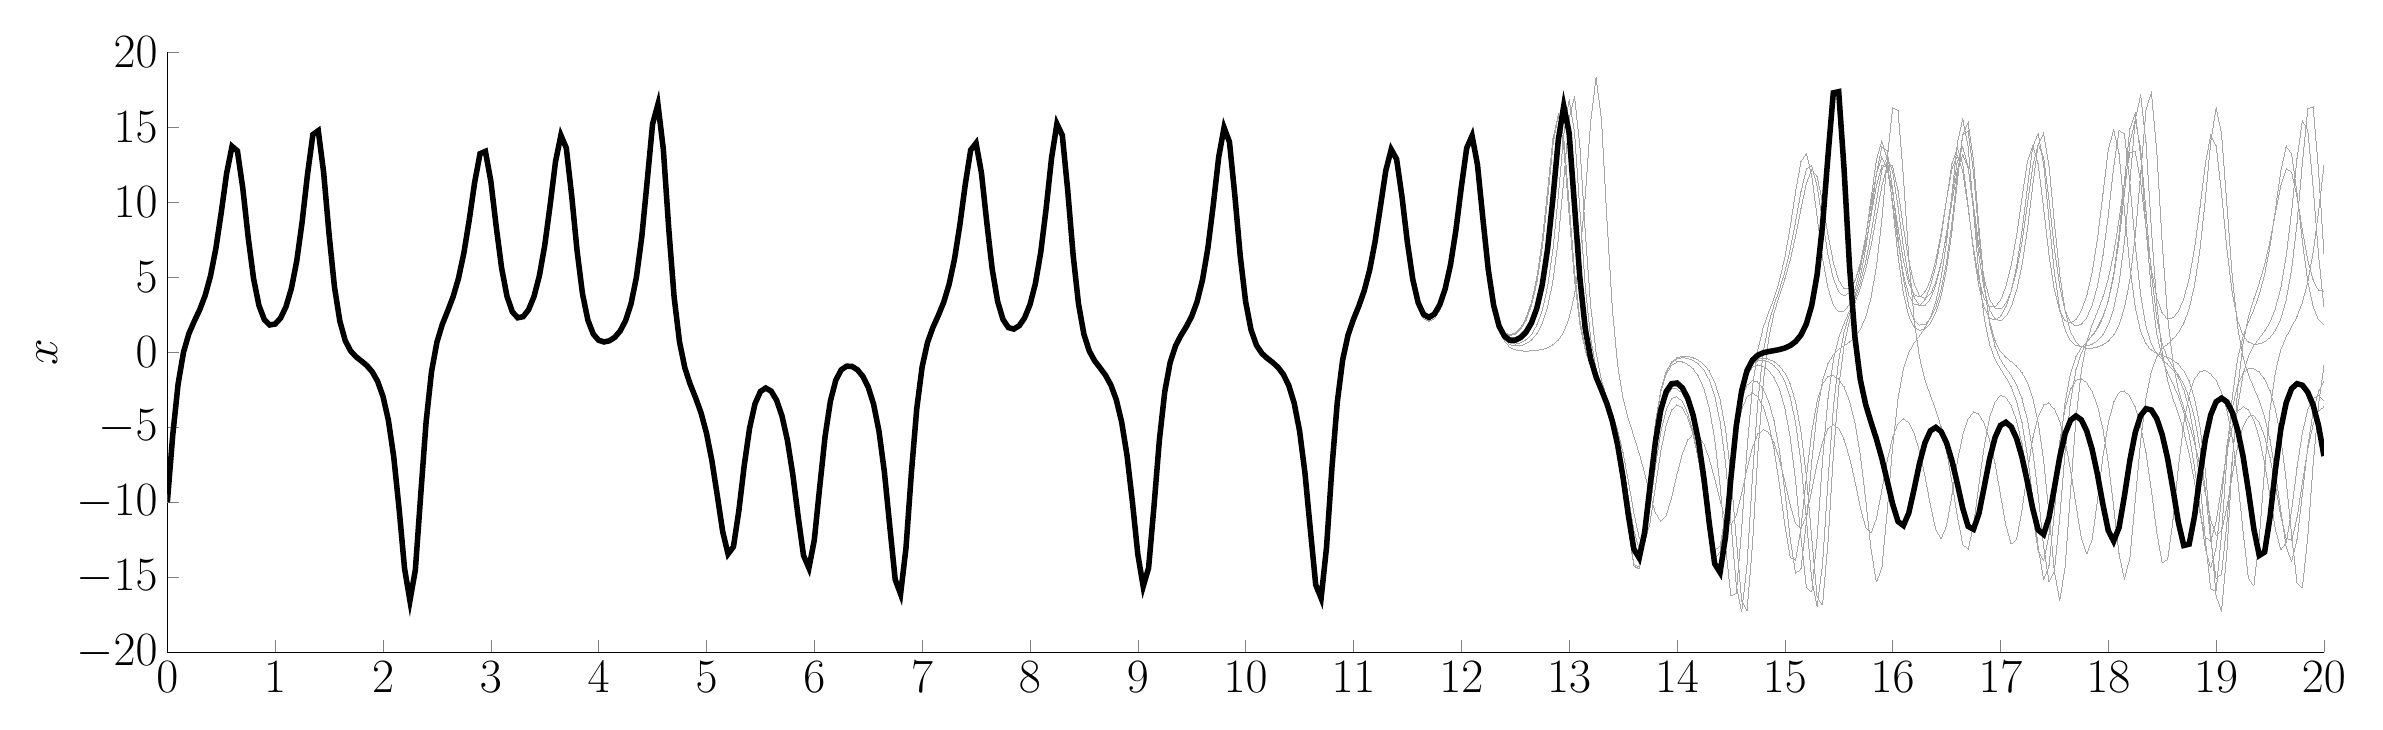
\begin{tikzpicture}

\begin{axis}[%
width=10.783in,
height=3in,
at={(1.809in,1.132in)},
scale only axis,
xmin=0,
xmax=20,
ymin=-20,
ymax=20,
axis background/.style={fill=white},
axis x line*=bottom,
axis y line*=left,
ylabel = {$x$},
ylabel style = {font=\LARGE},
ticklabel style={font=\LARGE},legend style={font=\LARGE},title style={font=\LARGE}
]
\addplot [color=white!65!black,solid,line width=0.0pt,forget plot]
  table[row sep=crcr]{%
0	-10\\
0.05	-5.53726\\
0.1	-2.11573\\
0.15	0.00290185\\
0.2	1.243\\
0.25	2.07127\\
0.3	2.83212\\
0.35	3.76911\\
0.4	5.07637\\
0.45	6.91238\\
0.5	9.31371\\
0.55	11.9319\\
0.6	13.7307\\
0.65	13.4256\\
0.7	10.939\\
0.75	7.6592\\
0.8	4.90597\\
0.85	3.11777\\
0.9	2.17349\\
0.95	1.82389\\
1	1.88526\\
1.05	2.28038\\
1.1	3.03009\\
1.15	4.23953\\
1.2	6.07584\\
1.25	8.67801\\
1.3	11.8547\\
1.35	14.5188\\
1.4	14.7739\\
1.45	11.9736\\
1.5	7.86494\\
1.55	4.36306\\
1.6	2.07385\\
1.65	0.779623\\
1.7	0.0912073\\
1.75	-0.297369\\
1.8	-0.580875\\
1.85	-0.882299\\
1.9	-1.29757\\
1.95	-1.93266\\
2	-2.9359\\
2.05	-4.5252\\
2.1	-6.98077\\
2.15	-10.4717\\
2.2	-14.4101\\
2.25	-16.5548\\
2.3	-14.5195\\
2.35	-9.50439\\
2.4	-4.63478\\
2.45	-1.3018\\
2.5	0.670719\\
2.55	1.86014\\
2.6	2.75657\\
2.65	3.69883\\
2.7	4.92602\\
2.75	6.61407\\
2.8	8.82711\\
2.85	11.3163\\
2.9	13.24\\
2.95	13.3948\\
3	11.4189\\
3.05	8.38538\\
3.1	5.62454\\
3.15	3.73239\\
3.2	2.69504\\
3.25	2.30201\\
3.3	2.3757\\
3.35	2.83754\\
3.4	3.7082\\
3.45	5.08908\\
3.5	7.11599\\
3.55	9.80975\\
3.6	12.7058\\
3.65	14.4678\\
3.7	13.6221\\
3.75	10.445\\
3.8	6.76369\\
3.85	3.91259\\
3.9	2.14911\\
3.95	1.21714\\
4	0.803274\\
4.05	0.69067\\
4.1	0.768019\\
4.15	1.00336\\
4.2	1.42436\\
4.25	2.11464\\
4.3	3.22491\\
4.35	4.98752\\
4.4	7.68515\\
4.45	11.398\\
4.5	15.2112\\
4.55	16.5316\\
4.6	13.5273\\
4.65	8.26251\\
4.7	3.67817\\
4.75	0.691149\\
4.8	-1.05683\\
4.85	-2.14931\\
4.9	-3.0425\\
4.95	-4.04801\\
5	-5.38819\\
5.05	-7.21605\\
5.1	-9.53107\\
5.15	-11.9392\\
5.2	-13.4441\\
5.25	-12.9653\\
5.3	-10.5781\\
5.35	-7.55759\\
5.4	-5.04928\\
5.45	-3.43443\\
5.5	-2.61484\\
5.55	-2.38232\\
5.6	-2.59001\\
5.65	-3.19243\\
5.7	-4.23811\\
5.75	-5.84355\\
5.8	-8.11841\\
5.85	-10.9437\\
5.9	-13.5427\\
5.95	-14.3797\\
6	-12.512\\
6.05	-8.99153\\
6.1	-5.60438\\
6.15	-3.22329\\
6.2	-1.84405\\
6.25	-1.168\\
6.3	-0.922954\\
6.35	-0.944707\\
6.4	-1.16741\\
6.45	-1.60093\\
6.5	-2.32066\\
6.55	-3.47236\\
6.6	-5.27881\\
6.65	-7.99266\\
6.7	-11.6186\\
6.75	-15.1482\\
6.8	-16.1093\\
6.85	-13.0512\\
6.9	-8.04999\\
6.95	-3.7558\\
7	-0.964672\\
7.05	0.661168\\
7.1	1.6603\\
7.15	2.45503\\
7.2	3.33751\\
7.25	4.52774\\
7.3	6.21094\\
7.35	8.49411\\
7.4	11.1964\\
7.45	13.4827\\
7.5	13.9456\\
7.55	11.9529\\
7.6	8.62465\\
7.65	5.53215\\
7.7	3.39303\\
7.75	2.18408\\
7.8	1.64408\\
7.85	1.5455\\
7.9	1.76617\\
7.95	2.28522\\
8	3.16859\\
8.05	4.56004\\
8.1	6.65537\\
8.15	9.57181\\
8.2	12.9293\\
8.25	15.2284\\
8.3	14.4834\\
8.35	10.8197\\
8.4	6.52229\\
8.45	3.23864\\
8.5	1.21334\\
8.55	0.079742\\
8.6	-0.573965\\
8.65	-1.04549\\
8.7	-1.53263\\
8.75	-2.18721\\
8.8	-3.16518\\
8.85	-4.66141\\
8.9	-6.90371\\
8.95	-10.0081\\
9	-13.4896\\
9.05	-15.6056\\
9.1	-14.3343\\
9.15	-10.2309\\
9.2	-5.82348\\
9.25	-2.61182\\
9.3	-0.67399\\
9.35	0.425366\\
9.4	1.11428\\
9.45	1.69623\\
9.5	2.38271\\
9.55	3.35239\\
9.6	4.79528\\
9.65	6.91185\\
9.7	9.78543\\
9.75	12.9739\\
9.8	14.991\\
9.85	14.0749\\
9.9	10.5205\\
9.95	6.46498\\
10	3.38577\\
10.05	1.49565\\
10.1	0.459756\\
10.15	-0.0954721\\
10.2	-0.434648\\
10.25	-0.722625\\
10.3	-1.06993\\
10.35	-1.57545\\
10.4	-2.3618\\
10.45	-3.60662\\
10.5	-5.56081\\
10.55	-8.49019\\
10.6	-12.3266\\
10.65	-15.7773\\
10.7	-16.1102\\
10.75	-12.3404\\
10.8	-7.1129\\
10.85	-2.93651\\
10.9	-0.31362\\
10.95	1.21571\\
11	2.208\\
11.05	3.07664\\
11.1	4.10573\\
11.15	5.50569\\
11.2	7.4227\\
11.25	9.83304\\
11.3	12.2724\\
11.35	13.6438\\
11.4	12.8819\\
11.45	10.2513\\
11.5	7.15116\\
11.55	4.68047\\
11.6	3.13508\\
11.65	2.3704\\
11.7	2.16553\\
11.75	2.37483\\
11.8	2.95689\\
11.85	3.96472\\
11.9	5.52407\\
11.95	7.77132\\
12	10.6512\\
12.05	13.471\\
12.1	14.6523\\
12.15	12.9865\\
12.2	9.38101\\
12.25	5.77205\\
12.3	3.18823\\
12.35	1.66432\\
12.4	0.880569\\
12.45	0.531508\\
12.5	0.420811\\
12.55	0.448859\\
12.6	0.581706\\
12.65	0.830212\\
12.7	1.24405\\
12.75	1.91956\\
12.8	3.01967\\
12.85	4.79786\\
12.9	7.57857\\
12.95	11.503\\
13	15.637\\
13.05	17.0761\\
13.1	13.721\\
13.15	7.98438\\
13.2	3.11738\\
13.25	0.00161994\\
13.3	-1.8233\\
13.35	-3.00137\\
13.4	-4.01439\\
13.45	-5.17603\\
13.5	-6.67828\\
13.55	-8.57814\\
13.6	-10.6746\\
13.65	-12.3429\\
13.7	-12.6923\\
13.75	-11.3434\\
13.8	-8.95226\\
13.85	-6.56761\\
13.9	-4.81796\\
13.95	-3.82614\\
14	-3.48516\\
14.05	-3.67171\\
14.1	-4.33014\\
14.15	-5.47858\\
14.2	-7.16508\\
14.25	-9.34787\\
14.3	-11.6563\\
14.35	-13.1817\\
14.4	-12.892\\
14.45	-10.7481\\
14.5	-7.87786\\
14.55	-5.40917\\
14.6	-3.78028\\
14.65	-2.94179\\
14.7	-2.70896\\
14.75	-2.9432\\
14.8	-3.60121\\
14.85	-4.72932\\
14.9	-6.42876\\
14.95	-8.7562\\
15	-11.4688\\
15.05	-13.6461\\
15.1	-13.8692\\
15.15	-11.6651\\
15.2	-8.28816\\
15.25	-5.26511\\
15.3	-3.22074\\
15.35	-2.0866\\
15.4	-1.59522\\
15.45	-1.5269\\
15.5	-1.76883\\
15.55	-2.30787\\
15.6	-3.2163\\
15.65	-4.64345\\
15.7	-6.78803\\
15.75	-9.75705\\
15.8	-13.1236\\
15.85	-15.3114\\
15.9	-14.3625\\
15.95	-10.5724\\
16	-6.28191\\
16.05	-3.06027\\
16.1	-1.09055\\
16.15	0.0115172\\
16.2	0.656289\\
16.25	1.13725\\
16.3	1.65086\\
16.35	2.35162\\
16.4	3.40176\\
16.45	5.00267\\
16.5	7.37575\\
16.55	10.5772\\
16.6	13.9494\\
16.65	15.5856\\
16.7	13.7471\\
16.75	9.47772\\
16.8	5.2559\\
16.85	2.29574\\
16.9	0.542254\\
16.95	-0.449782\\
17	-1.0828\\
17.05	-1.63601\\
17.1	-2.3058\\
17.15	-3.26376\\
17.2	-4.69923\\
17.25	-6.81934\\
17.3	-9.7241\\
17.35	-12.9914\\
17.4	-15.114\\
17.45	-14.2355\\
17.5	-10.6084\\
17.55	-6.44619\\
17.6	-3.28716\\
17.65	-1.34686\\
17.7	-0.272965\\
17.75	0.324939\\
17.8	0.725654\\
17.85	1.10893\\
17.9	1.60527\\
17.95	2.34309\\
18	3.48683\\
18.05	5.25993\\
18.1	7.90716\\
18.15	11.4366\\
18.2	14.9062\\
18.25	15.9725\\
18.3	13.1499\\
18.35	8.31084\\
18.4	4.05833\\
18.45	1.25921\\
18.5	-0.37155\\
18.55	-1.35173\\
18.6	-2.09636\\
18.65	-2.8929\\
18.7	-3.95823\\
18.75	-5.48594\\
18.8	-7.6333\\
18.85	-10.3654\\
18.9	-13.0763\\
18.95	-14.3536\\
19	-13.0096\\
19.05	-9.71104\\
19.1	-6.23841\\
19.15	-3.67075\\
19.2	-2.13312\\
19.25	-1.35837\\
19.3	-1.0651\\
19.35	-1.07359\\
19.4	-1.30767\\
19.45	-1.77357\\
19.5	-2.54844\\
19.55	-3.78263\\
19.6	-5.69924\\
19.65	-8.52345\\
19.7	-12.1488\\
19.75	-15.3572\\
19.8	-15.7027\\
19.85	-12.2846\\
19.9	-7.41775\\
19.95	-3.43692\\
20	-0.902631\\
};
\addplot [color=white!65!black,solid,line width=0.0pt,forget plot]
  table[row sep=crcr]{%
0	-10\\
0.05	-5.53725\\
0.1	-2.11573\\
0.15	0.00290251\\
0.2	1.243\\
0.25	2.07128\\
0.3	2.83212\\
0.35	3.76912\\
0.4	5.07637\\
0.45	6.91239\\
0.5	9.31372\\
0.55	11.932\\
0.6	13.7307\\
0.65	13.4256\\
0.7	10.939\\
0.75	7.65919\\
0.8	4.90597\\
0.85	3.11777\\
0.9	2.17349\\
0.95	1.82389\\
1	1.88527\\
1.05	2.28039\\
1.1	3.0301\\
1.15	4.23955\\
1.2	6.07587\\
1.25	8.67804\\
1.3	11.8548\\
1.35	14.5188\\
1.4	14.7739\\
1.45	11.9735\\
1.5	7.8649\\
1.55	4.36303\\
1.6	2.07384\\
1.65	0.779622\\
1.7	0.0912115\\
1.75	-0.297362\\
1.8	-0.580863\\
1.85	-0.88228\\
1.9	-1.29754\\
1.95	-1.93262\\
2	-2.93584\\
2.05	-4.52512\\
2.1	-6.98066\\
2.15	-10.4716\\
2.2	-14.41\\
2.25	-16.5548\\
2.3	-14.5197\\
2.35	-9.50459\\
2.4	-4.63492\\
2.45	-1.30186\\
2.5	0.670691\\
2.55	1.86013\\
2.6	2.75657\\
2.65	3.69883\\
2.7	4.92602\\
2.75	6.61406\\
2.8	8.82708\\
2.85	11.3162\\
2.9	13.24\\
2.95	13.3948\\
3	11.4189\\
3.05	8.38542\\
3.1	5.62459\\
3.15	3.73244\\
3.2	2.69509\\
3.25	2.30206\\
3.3	2.37575\\
3.35	2.8376\\
3.4	3.70827\\
3.45	5.08918\\
3.5	7.1161\\
3.55	9.80986\\
3.6	12.7059\\
3.65	14.4678\\
3.7	13.622\\
3.75	10.4449\\
3.8	6.76359\\
3.85	3.91255\\
3.9	2.14912\\
3.95	1.21718\\
4	0.803345\\
4.05	0.690772\\
4.1	0.768159\\
4.15	1.00356\\
4.2	1.42464\\
4.25	2.11507\\
4.3	3.22555\\
4.35	4.98848\\
4.4	7.68651\\
4.45	11.3996\\
4.5	15.2123\\
4.55	16.531\\
4.6	13.5253\\
4.65	8.26045\\
4.7	3.6768\\
4.75	0.690443\\
4.8	-1.05712\\
4.85	-2.14942\\
4.9	-3.04255\\
4.95	-4.04809\\
5	-5.38836\\
5.05	-7.21637\\
5.1	-9.53155\\
5.15	-11.9397\\
5.2	-13.4444\\
5.25	-12.9652\\
5.3	-10.5776\\
5.35	-7.55692\\
5.4	-5.04865\\
5.45	-3.4339\\
5.5	-2.6144\\
5.55	-2.38192\\
5.6	-2.58962\\
5.65	-3.192\\
5.7	-4.23762\\
5.75	-5.84298\\
5.8	-8.1178\\
5.85	-10.9432\\
5.9	-13.5426\\
5.95	-14.3802\\
6	-12.5128\\
6.05	-8.9922\\
6.1	-5.60465\\
6.15	-3.22321\\
6.2	-1.84372\\
6.25	-1.16747\\
6.3	-0.922241\\
6.35	-0.943753\\
6.4	-1.1661\\
6.45	-1.59907\\
6.5	-2.31796\\
6.55	-3.46837\\
6.6	-5.27297\\
6.65	-7.98463\\
6.7	-11.6094\\
6.75	-15.1426\\
6.8	-16.1132\\
6.85	-13.0627\\
6.9	-8.06139\\
6.95	-3.76317\\
7	-0.968296\\
7.05	0.659893\\
7.1	1.66021\\
7.15	2.4554\\
7.2	3.33791\\
7.25	4.5279\\
7.3	6.21055\\
7.35	8.49288\\
7.4	11.1942\\
7.45	13.4801\\
7.5	13.9442\\
7.55	11.9537\\
7.6	8.62715\\
7.65	5.53525\\
7.7	3.39612\\
7.75	2.18705\\
7.8	1.64709\\
7.85	1.54886\\
7.9	1.77025\\
7.95	2.29051\\
8	3.17574\\
8.05	4.56981\\
8.1	6.66835\\
8.15	9.58717\\
8.2	12.9422\\
8.25	15.2293\\
8.3	14.4686\\
8.35	10.799\\
8.4	6.50657\\
8.45	3.23062\\
8.5	1.21133\\
8.55	0.0815477\\
8.6	-0.569711\\
8.65	-1.03928\\
8.7	-1.52427\\
8.75	-2.17593\\
8.8	-3.14972\\
8.85	-4.64015\\
8.9	-6.87553\\
8.95	-9.97542\\
9	-13.4643\\
9.05	-15.6086\\
9.1	-14.3701\\
9.15	-10.2747\\
9.2	-5.85396\\
9.25	-2.62571\\
9.3	-0.675796\\
9.35	0.430987\\
9.4	1.12463\\
9.45	1.71041\\
9.5	2.40112\\
9.55	3.37629\\
9.6	4.82624\\
9.65	6.95038\\
9.7	9.82704\\
9.75	13.0027\\
9.8	14.983\\
9.85	14.0276\\
9.9	10.4649\\
9.95	6.42807\\
10	3.37213\\
10.05	1.4996\\
10.1	0.475486\\
10.15	-0.0708016\\
10.2	-0.400819\\
10.25	-0.676677\\
10.3	-1.00594\\
10.35	-1.48354\\
10.4	-2.22647\\
10.45	-3.40486\\
10.5	-5.26365\\
10.55	-8.08119\\
10.6	-11.871\\
10.65	-15.5308\\
10.7	-16.3649\\
10.75	-12.9431\\
10.8	-7.66571\\
10.85	-3.27708\\
10.9	-0.473901\\
10.95	1.16233\\
11	2.20459\\
11.05	3.0881\\
11.1	4.11041\\
11.15	5.48704\\
11.2	7.36522\\
11.25	9.72699\\
11.3	12.1337\\
11.35	13.5353\\
11.4	12.8774\\
11.45	10.3565\\
11.5	7.31102\\
11.55	4.84587\\
11.6	3.28763\\
11.65	2.5125\\
11.7	2.30819\\
11.75	2.53179\\
11.8	3.14309\\
11.85	4.19553\\
11.9	5.81081\\
11.95	8.10511\\
12	10.965\\
12.05	13.606\\
12.1	14.458\\
12.15	12.5523\\
12.2	8.97113\\
12.25	5.53912\\
12.3	3.13424\\
12.35	1.74113\\
12.4	1.05041\\
12.45	0.782337\\
12.5	0.766151\\
12.55	0.92781\\
12.6	1.2648\\
12.65	1.83349\\
12.7	2.75268\\
12.75	4.21764\\
12.8	6.49628\\
12.85	9.79881\\
12.9	13.7393\\
12.95	16.3908\\
13	15.1352\\
13.05	10.4486\\
13.1	5.42709\\
13.15	1.83233\\
13.2	-0.327073\\
13.25	-1.60432\\
13.3	-2.5115\\
13.35	-3.40876\\
13.4	-4.54826\\
13.45	-6.12078\\
13.5	-8.23288\\
13.55	-10.7425\\
13.6	-12.9566\\
13.65	-13.6468\\
13.7	-12.1016\\
13.75	-9.12796\\
13.8	-6.16658\\
13.85	-4.02175\\
13.9	-2.77857\\
13.95	-2.23469\\
14	-2.18681\\
14.05	-2.52582\\
14.1	-3.24531\\
14.15	-4.42729\\
14.2	-6.21306\\
14.25	-8.70819\\
14.3	-11.6987\\
14.35	-14.1648\\
14.4	-14.4118\\
14.45	-11.8632\\
14.5	-8.05315\\
14.55	-4.73998\\
14.6	-2.54509\\
14.65	-1.31431\\
14.7	-0.70769\\
14.75	-0.454031\\
14.8	-0.392897\\
14.85	-0.44933\\
14.9	-0.604492\\
14.95	-0.879361\\
15	-1.33291\\
15.05	-2.07332\\
15.1	-3.28061\\
15.15	-5.22906\\
15.2	-8.24586\\
15.25	-12.3657\\
15.3	-16.2881\\
15.35	-16.8414\\
15.4	-12.6786\\
15.45	-6.87682\\
15.5	-2.32031\\
15.55	0.50531\\
15.6	2.16566\\
15.65	3.28839\\
15.7	4.32057\\
15.75	5.54797\\
15.8	7.13464\\
15.85	9.08787\\
15.9	11.1166\\
15.95	12.5087\\
16	12.4386\\
16.05	10.7811\\
16.1	8.35467\\
16.15	6.12988\\
16.2	4.59076\\
16.25	3.7841\\
16.3	3.59234\\
16.35	3.90951\\
16.4	4.70082\\
16.45	5.99498\\
16.5	7.82252\\
16.55	10.0642\\
16.6	12.1972\\
16.65	13.2153\\
16.7	12.3123\\
16.75	9.86501\\
16.8	7.09318\\
16.85	4.9094\\
16.9	3.56484\\
16.95	2.94957\\
17	2.89127\\
17.05	3.28519\\
17.1	4.12079\\
17.15	5.46529\\
17.2	7.40801\\
17.25	9.90719\\
17.3	12.4688\\
17.35	13.9046\\
17.4	13.0527\\
17.45	10.2284\\
17.5	6.96251\\
17.55	4.40119\\
17.6	2.81307\\
17.65	2.016\\
17.7	1.7631\\
17.75	1.89145\\
17.8	2.34474\\
17.85	3.16144\\
17.9	4.46159\\
17.95	6.42057\\
18	9.15767\\
18.05	12.3817\\
18.1	14.8153\\
18.15	14.5542\\
18.2	11.3529\\
18.25	7.20593\\
18.3	3.86584\\
18.35	1.7484\\
18.4	0.567296\\
18.45	-0.0678897\\
18.5	-0.448643\\
18.55	-0.759777\\
18.6	-1.12378\\
18.65	-1.64625\\
18.7	-2.45375\\
18.75	-3.72593\\
18.8	-5.71171\\
18.85	-8.66233\\
18.9	-12.4657\\
18.95	-15.7701\\
19	-15.9075\\
19.05	-12.0906\\
19.1	-6.96835\\
19.15	-2.9171\\
19.2	-0.381898\\
19.25	1.09323\\
19.3	2.04781\\
19.35	2.8817\\
19.4	3.87165\\
19.45	5.22848\\
19.5	7.11288\\
19.55	9.54224\\
19.6	12.1185\\
19.65	13.7593\\
19.7	13.2439\\
19.75	10.6496\\
19.8	7.40542\\
19.85	4.7507\\
19.9	3.05616\\
19.95	2.18131\\
20	1.88292\\
};
\addplot [color=white!65!black,solid,line width=0.0pt,forget plot]
  table[row sep=crcr]{%
0	-10\\
0.05	-5.53726\\
0.1	-2.11573\\
0.15	0.00290269\\
0.2	1.243\\
0.25	2.07127\\
0.3	2.83212\\
0.35	3.76911\\
0.4	5.07637\\
0.45	6.91238\\
0.5	9.31371\\
0.55	11.932\\
0.6	13.7307\\
0.65	13.4256\\
0.7	10.939\\
0.75	7.6592\\
0.8	4.90597\\
0.85	3.11777\\
0.9	2.17349\\
0.95	1.82389\\
1	1.88527\\
1.05	2.28039\\
1.1	3.03009\\
1.15	4.23954\\
1.2	6.07585\\
1.25	8.67802\\
1.3	11.8547\\
1.35	14.5188\\
1.4	14.7739\\
1.45	11.9735\\
1.5	7.86492\\
1.55	4.36305\\
1.6	2.07385\\
1.65	0.779623\\
1.7	0.0912114\\
1.75	-0.297364\\
1.8	-0.580865\\
1.85	-0.882282\\
1.9	-1.29754\\
1.95	-1.93263\\
2	-2.93585\\
2.05	-4.52513\\
2.1	-6.98067\\
2.15	-10.4716\\
2.2	-14.41\\
2.25	-16.5548\\
2.3	-14.5197\\
2.35	-9.50456\\
2.4	-4.6349\\
2.45	-1.30186\\
2.5	0.670692\\
2.55	1.86013\\
2.6	2.75657\\
2.65	3.69883\\
2.7	4.92602\\
2.75	6.61406\\
2.8	8.82709\\
2.85	11.3162\\
2.9	13.24\\
2.95	13.3948\\
3	11.4189\\
3.05	8.38542\\
3.1	5.62459\\
3.15	3.73244\\
3.2	2.69508\\
3.25	2.30206\\
3.3	2.37575\\
3.35	2.8376\\
3.4	3.70826\\
3.45	5.08917\\
3.5	7.11608\\
3.55	9.80984\\
3.6	12.7059\\
3.65	14.4678\\
3.7	13.622\\
3.75	10.4449\\
3.8	6.76361\\
3.85	3.91256\\
3.9	2.14912\\
3.95	1.21718\\
4	0.80334\\
4.05	0.690764\\
4.1	0.768144\\
4.15	1.00354\\
4.2	1.42462\\
4.25	2.11503\\
4.3	3.22549\\
4.35	4.9884\\
4.4	7.6864\\
4.45	11.3995\\
4.5	15.2122\\
4.55	16.5311\\
4.6	13.5255\\
4.65	8.26062\\
4.7	3.67692\\
4.75	0.690505\\
4.8	-1.05709\\
4.85	-2.1494\\
4.9	-3.04253\\
4.95	-4.04808\\
5	-5.38834\\
5.05	-7.21633\\
5.1	-9.5315\\
5.15	-11.9397\\
5.2	-13.4444\\
5.25	-12.9653\\
5.3	-10.5777\\
5.35	-7.55698\\
5.4	-5.0487\\
5.45	-3.43394\\
5.5	-2.61443\\
5.55	-2.38194\\
5.6	-2.58963\\
5.65	-3.19202\\
5.7	-4.23763\\
5.75	-5.84299\\
5.8	-8.11781\\
5.85	-10.9432\\
5.9	-13.5426\\
5.95	-14.3802\\
6	-12.5128\\
6.05	-8.9922\\
6.1	-5.60466\\
6.15	-3.22323\\
6.2	-1.84374\\
6.25	-1.1675\\
6.3	-0.922269\\
6.35	-0.943787\\
6.4	-1.16615\\
6.45	-1.59914\\
6.5	-2.31805\\
6.55	-3.46851\\
6.6	-5.27317\\
6.65	-7.9849\\
6.7	-11.6098\\
6.75	-15.1428\\
6.8	-16.1131\\
6.85	-13.0623\\
6.9	-8.06101\\
6.95	-3.76293\\
7	-0.968176\\
7.05	0.659931\\
7.1	1.6602\\
7.15	2.45538\\
7.2	3.33788\\
7.25	4.52787\\
7.3	6.21055\\
7.35	8.4929\\
7.4	11.1943\\
7.45	13.4802\\
7.5	13.9442\\
7.55	11.9537\\
7.6	8.62709\\
7.65	5.53516\\
7.7	3.39601\\
7.75	2.18694\\
7.8	1.64697\\
7.85	1.54872\\
7.9	1.77008\\
7.95	2.29028\\
8	3.17543\\
8.05	4.56939\\
8.1	6.66778\\
8.15	9.58649\\
8.2	12.9416\\
8.25	15.2292\\
8.3	14.4692\\
8.35	10.7999\\
8.4	6.50727\\
8.45	3.23098\\
8.5	1.21144\\
8.55	0.0814906\\
8.6	-0.569875\\
8.65	-1.03952\\
8.7	-1.5246\\
8.75	-2.17637\\
8.8	-3.15032\\
8.85	-4.64098\\
8.9	-6.87663\\
8.95	-9.97669\\
9	-13.4653\\
9.05	-15.6085\\
9.1	-14.3687\\
9.15	-10.273\\
9.2	-5.85278\\
9.25	-2.62519\\
9.3	-0.675746\\
9.35	0.430747\\
9.4	1.1242\\
9.45	1.70983\\
9.5	2.40037\\
9.55	3.37531\\
9.6	4.82496\\
9.65	6.94878\\
9.7	9.82532\\
9.75	13.0015\\
9.8	14.9833\\
9.85	14.0295\\
9.9	10.4672\\
9.95	6.42961\\
10	3.37272\\
10.05	1.49946\\
10.1	0.474862\\
10.15	-0.0717895\\
10.2	-0.402184\\
10.25	-0.67853\\
10.3	-1.00852\\
10.35	-1.48726\\
10.4	-2.23194\\
10.45	-3.41304\\
10.5	-5.27573\\
10.55	-8.09797\\
10.6	-11.8901\\
10.65	-15.542\\
10.7	-16.3555\\
10.75	-12.9182\\
10.8	-7.64223\\
10.85	-3.26236\\
10.9	-0.46685\\
10.95	1.16478\\
11	2.20489\\
11.05	3.08775\\
11.1	4.11034\\
11.15	5.48797\\
11.2	7.36779\\
11.25	9.73157\\
11.3	12.1396\\
11.35	13.5399\\
11.4	12.8775\\
11.45	10.352\\
11.5	7.30422\\
11.55	4.8389\\
11.6	3.28128\\
11.65	2.50667\\
11.7	2.30242\\
11.75	2.52553\\
11.8	3.13575\\
11.85	4.18654\\
11.9	5.79981\\
11.95	8.09257\\
12	10.9537\\
12.05	13.602\\
12.1	14.4663\\
12.15	12.5688\\
12.2	8.98594\\
12.25	5.54703\\
12.3	3.13546\\
12.35	1.73749\\
12.4	1.04324\\
12.45	0.771983\\
12.5	0.751965\\
12.55	0.908141\\
12.6	1.23675\\
12.65	1.79234\\
12.7	2.69116\\
12.75	4.12533\\
12.8	6.36177\\
12.85	9.62285\\
12.9	13.573\\
12.95	16.3606\\
13	15.3064\\
13.05	10.6954\\
13.1	5.61777\\
13.15	1.94022\\
13.2	-0.278484\\
13.25	-1.58757\\
13.3	-2.5075\\
13.35	-3.4058\\
13.4	-4.53852\\
13.45	-6.09778\\
13.5	-8.19148\\
13.55	-10.6839\\
13.6	-12.8987\\
13.65	-13.6237\\
13.7	-12.1322\\
13.75	-9.1946\\
13.8	-6.24066\\
13.85	-4.08777\\
13.9	-2.8344\\
13.95	-2.28421\\
14	-2.2354\\
14.05	-2.57878\\
14.1	-3.30772\\
14.15	-4.50371\\
14.2	-6.30551\\
14.25	-8.80946\\
14.3	-11.7795\\
14.35	-14.1719\\
14.4	-14.3188\\
14.45	-11.7259\\
14.5	-7.94824\\
14.55	-4.69484\\
14.6	-2.55082\\
14.65	-1.35571\\
14.7	-0.775975\\
14.75	-0.548857\\
14.8	-0.521968\\
14.85	-0.629063\\
14.9	-0.863001\\
14.95	-1.26265\\
15	-1.91534\\
15.05	-2.97276\\
15.1	-4.67214\\
15.15	-7.32079\\
15.2	-11.0772\\
15.25	-15.1615\\
15.3	-16.9284\\
15.35	-14.0989\\
15.4	-8.60332\\
15.45	-3.70203\\
15.5	-0.488649\\
15.55	1.39683\\
15.6	2.58078\\
15.65	3.55294\\
15.7	4.64073\\
15.75	6.0602\\
15.8	7.92225\\
15.85	10.1288\\
15.9	12.1619\\
15.95	13.0599\\
16	12.1083\\
16.05	9.72096\\
16.1	7.05983\\
16.15	4.97591\\
16.2	3.70341\\
16.25	3.14219\\
16.3	3.13519\\
16.35	3.59024\\
16.4	4.50421\\
16.45	5.94165\\
16.5	7.96397\\
16.55	10.4483\\
16.6	12.7685\\
16.65	13.7121\\
16.7	12.4139\\
16.75	9.51247\\
16.8	6.47112\\
16.85	4.202\\
16.9	2.85246\\
16.95	2.23127\\
17	2.12464\\
17.05	2.4088\\
17.1	3.06385\\
17.15	4.16093\\
17.2	5.83801\\
17.25	8.22381\\
17.3	11.1949\\
17.35	13.8923\\
17.4	14.6297\\
17.45	12.4719\\
17.5	8.6923\\
17.55	5.19099\\
17.6	2.78911\\
17.65	1.40853\\
17.7	0.70781\\
17.75	0.392895\\
17.8	0.281316\\
17.85	0.280346\\
17.9	0.35449\\
17.95	0.504208\\
18	0.757942\\
18.05	1.17556\\
18.1	1.86249\\
18.15	2.9947\\
18.2	4.84761\\
18.25	7.7765\\
18.3	11.9269\\
18.35	16.2054\\
18.4	17.3559\\
18.45	13.401\\
18.5	7.31513\\
18.55	2.39937\\
18.6	-0.672279\\
18.65	-2.47218\\
18.7	-3.67109\\
18.75	-4.74489\\
18.8	-5.985\\
18.85	-7.53562\\
18.9	-9.36048\\
18.95	-11.1306\\
19	-12.1865\\
19.05	-11.8963\\
19.1	-10.2946\\
19.15	-8.13118\\
19.2	-6.20208\\
19.25	-4.89668\\
19.3	-4.2589\\
19.35	-4.20322\\
19.4	-4.65356\\
19.45	-5.58675\\
19.5	-7.0098\\
19.55	-8.87119\\
19.6	-10.8887\\
19.65	-12.3871\\
19.7	-12.518\\
19.75	-11.0346\\
19.8	-8.66107\\
19.85	-6.38858\\
19.9	-4.76578\\
19.95	-3.87992\\
20	-3.62383\\
};
\addplot [color=white!65!black,solid,line width=0.0pt,forget plot]
  table[row sep=crcr]{%
0	-10\\
0.05	-5.53726\\
0.1	-2.11573\\
0.15	0.00290209\\
0.2	1.243\\
0.25	2.07127\\
0.3	2.83212\\
0.35	3.76911\\
0.4	5.07636\\
0.45	6.91238\\
0.5	9.31371\\
0.55	11.9319\\
0.6	13.7307\\
0.65	13.4256\\
0.7	10.939\\
0.75	7.6592\\
0.8	4.90597\\
0.85	3.11777\\
0.9	2.17348\\
0.95	1.82389\\
1	1.88526\\
1.05	2.28037\\
1.1	3.03008\\
1.15	4.23952\\
1.2	6.07583\\
1.25	8.678\\
1.3	11.8547\\
1.35	14.5188\\
1.4	14.7739\\
1.45	11.9736\\
1.5	7.86496\\
1.55	4.36307\\
1.6	2.07385\\
1.65	0.779619\\
1.7	0.0911986\\
1.75	-0.297382\\
1.8	-0.58089\\
1.85	-0.882318\\
1.9	-1.2976\\
1.95	-1.93271\\
2	-2.93596\\
2.05	-4.5253\\
2.1	-6.98091\\
2.15	-10.4719\\
2.2	-14.4103\\
2.25	-16.5548\\
2.3	-14.5194\\
2.35	-9.50416\\
2.4	-4.63462\\
2.45	-1.30171\\
2.5	0.670756\\
2.55	1.86015\\
2.6	2.75657\\
2.65	3.69883\\
2.7	4.92603\\
2.75	6.61409\\
2.8	8.82715\\
2.85	11.3163\\
2.9	13.2401\\
2.95	13.3948\\
3	11.4189\\
3.05	8.38532\\
3.1	5.62448\\
3.15	3.73234\\
3.2	2.69499\\
3.25	2.30197\\
3.3	2.37566\\
3.35	2.8375\\
3.4	3.70815\\
3.45	5.08902\\
3.5	7.11592\\
3.55	9.80968\\
3.6	12.7058\\
3.65	14.4679\\
3.7	13.6222\\
3.75	10.4451\\
3.8	6.76375\\
3.85	3.91261\\
3.9	2.14909\\
3.95	1.2171\\
4	0.803215\\
4.05	0.690593\\
4.1	0.767911\\
4.15	1.00321\\
4.2	1.42414\\
4.25	2.11431\\
4.3	3.22441\\
4.35	4.98677\\
4.4	7.68409\\
4.45	11.3967\\
4.5	15.2103\\
4.55	16.532\\
4.6	13.5289\\
4.65	8.26413\\
4.7	3.67924\\
4.75	0.691701\\
4.8	-1.05659\\
4.85	-2.14923\\
4.9	-3.04246\\
4.95	-4.04795\\
5	-5.38804\\
5.05	-7.21578\\
5.1	-9.53066\\
5.15	-11.9387\\
5.2	-13.4438\\
5.25	-12.9654\\
5.3	-10.5785\\
5.35	-7.55813\\
5.4	-5.04979\\
5.45	-3.43485\\
5.5	-2.61518\\
5.55	-2.38262\\
5.6	-2.59031\\
5.65	-3.19276\\
5.7	-4.23848\\
5.75	-5.84398\\
5.8	-8.11886\\
5.85	-10.9441\\
5.9	-13.5427\\
5.95	-14.3793\\
6	-12.5113\\
6.05	-8.99105\\
6.1	-5.60419\\
6.15	-3.22337\\
6.2	-1.84432\\
6.25	-1.1684\\
6.3	-0.923504\\
6.35	-0.945444\\
6.4	-1.16842\\
6.45	-1.60236\\
6.5	-2.32274\\
6.55	-3.47543\\
6.6	-5.28329\\
6.65	-7.99882\\
6.7	-11.6256\\
6.75	-15.1525\\
6.8	-16.1063\\
6.85	-13.0423\\
6.9	-8.04125\\
6.95	-3.75015\\
7	-0.961903\\
7.05	0.662136\\
7.1	1.66036\\
7.15	2.45474\\
7.2	3.33718\\
7.25	4.52761\\
7.3	6.21122\\
7.35	8.49503\\
7.4	11.1981\\
7.45	13.4847\\
7.5	13.9467\\
7.55	11.9523\\
7.6	8.62278\\
7.65	5.5298\\
7.7	3.39068\\
7.75	2.18182\\
7.8	1.64176\\
7.85	1.54292\\
7.9	1.76303\\
7.95	2.28114\\
8	3.1631\\
8.05	4.55252\\
8.1	6.64536\\
8.15	9.55996\\
8.2	12.9194\\
8.25	15.2277\\
8.3	14.4949\\
8.35	10.8356\\
8.4	6.53446\\
8.45	3.24487\\
8.5	1.21493\\
8.55	0.0783758\\
8.6	-0.577218\\
8.65	-1.05025\\
8.7	-1.53905\\
8.75	-2.19585\\
8.8	-3.17701\\
8.85	-4.67765\\
8.9	-6.92521\\
8.95	-10.033\\
9	-13.5087\\
9.05	-15.6029\\
9.1	-14.307\\
9.15	-10.1978\\
9.2	-5.80045\\
9.25	-2.60141\\
9.3	-0.672743\\
9.35	0.42097\\
9.4	1.10628\\
9.45	1.68528\\
9.5	2.36847\\
9.55	3.33388\\
9.6	4.77122\\
9.65	6.88182\\
9.7	9.75279\\
9.75	12.9509\\
9.8	14.9966\\
9.85	14.1116\\
9.9	10.5641\\
9.95	6.49428\\
10	3.39688\\
10.05	1.49299\\
10.1	0.447878\\
10.15	-0.114282\\
10.2	-0.460481\\
10.25	-0.757695\\
10.3	-1.11872\\
10.35	-1.6454\\
10.4	-2.46457\\
10.45	-3.75926\\
10.5	-5.78396\\
10.55	-8.79222\\
10.6	-12.6491\\
10.65	-15.9229\\
10.7	-15.8895\\
10.75	-11.8997\\
10.8	-6.72967\\
10.85	-2.70788\\
10.9	-0.210036\\
10.95	1.24655\\
11	2.20513\\
11.05	3.06372\\
11.1	4.09732\\
11.15	5.51314\\
11.2	7.45724\\
11.25	9.90275\\
11.3	12.3679\\
11.35	13.7222\\
11.4	12.89\\
11.45	10.1826\\
11.5	7.04204\\
11.55	4.56447\\
11.6	3.02511\\
11.65	2.26491\\
11.7	2.0566\\
11.75	2.25198\\
11.8	2.808\\
11.85	3.77626\\
11.9	5.28407\\
11.95	7.48166\\
12	10.3596\\
12.05	13.3099\\
12.1	14.7754\\
12.15	13.3535\\
12.2	9.7618\\
12.25	6.01019\\
12.3	3.26882\\
12.35	1.62792\\
12.4	0.76343\\
12.45	0.348868\\
12.5	0.166561\\
12.55	0.0963942\\
12.6	0.0803052\\
12.65	0.094421\\
12.7	0.13317\\
12.75	0.202427\\
12.8	0.31859\\
12.85	0.51228\\
12.9	0.837082\\
12.95	1.38547\\
13	2.31538\\
13.05	3.88813\\
13.1	6.4925\\
13.15	10.5014\\
13.2	15.4435\\
13.25	18.341\\
13.3	15.5333\\
13.35	8.94106\\
13.4	3.002\\
13.45	-0.829\\
13.5	-3.05126\\
13.55	-4.44098\\
13.6	-5.55665\\
13.65	-6.7155\\
13.7	-8.03865\\
13.75	-9.45358\\
13.8	-10.6699\\
13.85	-11.2476\\
13.9	-10.874\\
13.95	-9.66775\\
14	-8.12229\\
14.05	-6.74583\\
14.1	-5.82224\\
14.15	-5.42556\\
14.2	-5.53132\\
14.25	-6.09721\\
14.3	-7.08205\\
14.35	-8.40714\\
14.4	-9.87057\\
14.45	-11.0703\\
14.5	-11.4896\\
14.55	-10.8445\\
14.6	-9.38196\\
14.65	-7.69829\\
14.7	-6.30648\\
14.75	-5.44142\\
14.8	-5.13275\\
14.85	-5.3356\\
14.9	-6.00619\\
14.95	-7.10962\\
15	-8.56711\\
15.05	-10.1515\\
15.1	-11.398\\
15.15	-11.725\\
15.2	-10.8668\\
15.25	-9.18177\\
15.3	-7.36002\\
15.35	-5.92537\\
15.4	-5.07687\\
15.45	-4.80979\\
15.5	-5.06322\\
15.55	-5.79395\\
15.6	-6.97825\\
15.65	-8.55087\\
15.7	-10.2825\\
15.75	-11.6624\\
15.8	-12.0218\\
15.85	-11.0498\\
15.9	-9.16961\\
15.95	-7.1729\\
16	-5.62784\\
16.05	-4.72304\\
16.1	-4.42833\\
16.15	-4.66547\\
16.2	-5.38858\\
16.25	-6.58829\\
16.3	-8.2325\\
16.35	-10.1344\\
16.4	-11.7868\\
16.45	-12.413\\
16.5	-11.5274\\
16.55	-9.50684\\
16.6	-7.26214\\
16.65	-5.48442\\
16.7	-4.40382\\
16.75	-3.97752\\
16.8	-4.10198\\
16.85	-4.71587\\
16.9	-5.81731\\
16.95	-7.42179\\
17	-9.44614\\
17.05	-11.5033\\
17.1	-12.7737\\
17.15	-12.4213\\
17.2	-10.48\\
17.25	-7.91923\\
17.3	-5.70409\\
17.35	-4.23823\\
17.4	-3.50931\\
17.45	-3.37801\\
17.5	-3.73862\\
17.55	-4.56577\\
17.6	-5.90164\\
17.65	-7.79244\\
17.7	-10.1294\\
17.75	-12.3702\\
17.8	-13.4344\\
17.85	-12.4502\\
17.9	-9.84376\\
17.95	-6.93613\\
18	-4.67576\\
18.05	-3.29389\\
18.1	-2.65182\\
18.15	-2.55715\\
18.2	-2.89335\\
18.25	-3.6437\\
18.3	-4.87796\\
18.35	-6.71249\\
18.4	-9.19217\\
18.45	-11.9907\\
18.5	-14.0195\\
18.55	-13.8104\\
18.6	-11.1785\\
18.65	-7.64723\\
18.7	-4.68797\\
18.75	-2.76761\\
18.8	-1.73011\\
18.85	-1.28507\\
18.9	-1.21461\\
18.95	-1.4097\\
19	-1.85473\\
19.05	-2.61234\\
19.1	-3.8205\\
19.15	-5.6876\\
19.2	-8.42266\\
19.25	-11.9243\\
19.3	-15.0646\\
19.35	-15.5485\\
19.4	-12.4089\\
19.45	-7.72917\\
19.5	-3.80261\\
19.55	-1.26844\\
19.6	0.19225\\
19.65	1.06168\\
19.7	1.71494\\
19.75	2.41014\\
19.8	3.34578\\
19.85	4.71222\\
19.9	6.70114\\
19.95	9.40358\\
20	12.4654\\
};
\addplot [color=white!65!black,solid,line width=0.0pt,forget plot]
  table[row sep=crcr]{%
0	-10\\
0.05	-5.53726\\
0.1	-2.11573\\
0.15	0.00290342\\
0.2	1.243\\
0.25	2.07128\\
0.3	2.83212\\
0.35	3.76912\\
0.4	5.07637\\
0.45	6.91239\\
0.5	9.31372\\
0.55	11.932\\
0.6	13.7307\\
0.65	13.4256\\
0.7	10.939\\
0.75	7.65919\\
0.8	4.90596\\
0.85	3.11777\\
0.9	2.17348\\
0.95	1.82389\\
1	1.88527\\
1.05	2.28039\\
1.1	3.03009\\
1.15	4.23955\\
1.2	6.07586\\
1.25	8.67804\\
1.3	11.8548\\
1.35	14.5188\\
1.4	14.7739\\
1.45	11.9735\\
1.5	7.86491\\
1.55	4.36303\\
1.6	2.07384\\
1.65	0.779616\\
1.7	0.091205\\
1.75	-0.29737\\
1.8	-0.580874\\
1.85	-0.882296\\
1.9	-1.29756\\
1.95	-1.93266\\
2	-2.93589\\
2.05	-4.52519\\
2.1	-6.98076\\
2.15	-10.4717\\
2.2	-14.4101\\
2.25	-16.5548\\
2.3	-14.5196\\
2.35	-9.50441\\
2.4	-4.63479\\
2.45	-1.30179\\
2.5	0.670724\\
2.55	1.86015\\
2.6	2.75658\\
2.65	3.69885\\
2.7	4.92604\\
2.75	6.61409\\
2.8	8.82713\\
2.85	11.3163\\
2.9	13.24\\
2.95	13.3947\\
3	11.4189\\
3.05	8.38536\\
3.1	5.62454\\
3.15	3.7324\\
3.2	2.69505\\
3.25	2.30203\\
3.3	2.37573\\
3.35	2.83758\\
3.4	3.70824\\
3.45	5.08915\\
3.5	7.11607\\
3.55	9.80983\\
3.6	12.7059\\
3.65	14.4678\\
3.7	13.622\\
3.75	10.4449\\
3.8	6.76361\\
3.85	3.91255\\
3.9	2.1491\\
3.95	1.21715\\
4	0.803299\\
4.05	0.690711\\
4.1	0.768074\\
4.15	1.00344\\
4.2	1.42448\\
4.25	2.11482\\
4.3	3.22517\\
4.35	4.98792\\
4.4	7.68572\\
4.45	11.3987\\
4.5	15.2117\\
4.55	16.5314\\
4.6	13.5265\\
4.65	8.26165\\
4.7	3.67759\\
4.75	0.690844\\
4.8	-1.05696\\
4.85	-2.14937\\
4.9	-3.04253\\
4.95	-4.04806\\
5	-5.38828\\
5.05	-7.2162\\
5.1	-9.53128\\
5.15	-11.9394\\
5.2	-13.4442\\
5.25	-12.9653\\
5.3	-10.5779\\
5.35	-7.5573\\
5.4	-5.04902\\
5.45	-3.43422\\
5.5	-2.61467\\
5.55	-2.38216\\
5.6	-2.58986\\
5.65	-3.19228\\
5.7	-4.23793\\
5.75	-5.84335\\
5.8	-8.1182\\
5.85	-10.9436\\
5.9	-13.5427\\
5.95	-14.3799\\
6	-12.5123\\
6.05	-8.99175\\
6.1	-5.60445\\
6.15	-3.22324\\
6.2	-1.84391\\
6.25	-1.16779\\
6.3	-0.922676\\
6.35	-0.944338\\
6.4	-1.16691\\
6.45	-1.60021\\
6.5	-2.31961\\
6.55	-3.47083\\
6.6	-5.27656\\
6.65	-7.98957\\
6.7	-11.6151\\
6.75	-15.146\\
6.8	-16.1108\\
6.85	-13.0556\\
6.9	-8.05437\\
6.95	-3.75863\\
7	-0.966058\\
7.05	0.660688\\
7.1	1.66028\\
7.15	2.45519\\
7.2	3.33768\\
7.25	4.52782\\
7.3	6.21082\\
7.35	8.49367\\
7.4	11.1956\\
7.45	13.4817\\
7.5	13.945\\
7.55	11.9532\\
7.6	8.62558\\
7.65	5.53332\\
7.7	3.39421\\
7.75	2.18523\\
7.8	1.64525\\
7.85	1.54681\\
7.9	1.76776\\
7.95	2.28729\\
8	3.17139\\
8.05	4.56387\\
8.1	6.66046\\
8.15	9.57784\\
8.2	12.9344\\
8.25	15.2288\\
8.3	14.4776\\
8.35	10.8115\\
8.4	6.5161\\
8.45	3.23547\\
8.5	1.21254\\
8.55	0.0804323\\
8.6	-0.572318\\
8.65	-1.04308\\
8.7	-1.52939\\
8.75	-2.18283\\
8.8	-3.15918\\
8.85	-4.65317\\
8.9	-6.8928\\
8.95	-9.99549\\
9	-13.4799\\
9.05	-15.6068\\
9.1	-14.3482\\
9.15	-10.2478\\
9.2	-5.83523\\
9.25	-2.61715\\
9.3	-0.674648\\
9.35	0.427582\\
9.4	1.11833\\
9.45	1.70177\\
9.5	2.38991\\
9.55	3.36175\\
9.6	4.80741\\
9.65	6.92697\\
9.7	9.80181\\
9.75	12.9853\\
9.8	14.988\\
9.85	14.0564\\
9.9	10.4986\\
9.95	6.45039\\
10	3.38031\\
10.05	1.49712\\
10.1	0.465842\\
10.15	-0.0858873\\
10.2	-0.421496\\
10.25	-0.70476\\
10.3	-1.04506\\
10.35	-1.53975\\
10.4	-2.30928\\
10.45	-3.52842\\
10.5	-5.44592\\
10.55	-8.33296\\
10.6	-12.154\\
10.65	-15.6893\\
10.7	-16.2145\\
10.75	-12.5714\\
10.8	-7.32066\\
10.85	-3.06301\\
10.9	-0.372366\\
10.95	1.19685\\
11	2.20771\\
11.05	3.08187\\
11.1	4.10844\\
11.15	5.49967\\
11.2	7.40204\\
11.25	9.79385\\
11.3	12.2203\\
11.35	13.6025\\
11.4	12.8793\\
11.45	10.2902\\
11.5	7.21096\\
11.55	4.74288\\
11.6	3.19319\\
11.65	2.4251\\
11.7	2.22101\\
11.75	2.43642\\
11.8	3.03054\\
11.85	4.05673\\
11.9	5.63941\\
11.95	7.90733\\
12	10.7822\\
12.05	13.533\\
12.1	14.5801\\
12.15	12.8109\\
12.2	9.21009\\
12.25	5.67153\\
12.3	3.16082\\
12.35	1.69059\\
12.4	0.944601\\
12.45	0.627644\\
12.5	0.553644\\
12.55	0.63311\\
12.6	0.844403\\
12.65	1.21626\\
12.7	1.82625\\
12.75	2.8136\\
12.8	4.3996\\
12.85	6.88169\\
12.9	10.463\\
12.95	14.5748\\
13	16.8607\\
13.05	14.726\\
13.1	9.45562\\
13.15	4.39126\\
13.2	0.957843\\
13.25	-1.07027\\
13.3	-2.31053\\
13.35	-3.27412\\
13.4	-4.30806\\
13.45	-5.64564\\
13.5	-7.42788\\
13.55	-9.62486\\
13.6	-11.8273\\
13.65	-13.1146\\
13.7	-12.5784\\
13.75	-10.3561\\
13.8	-7.58582\\
13.85	-5.28111\\
13.9	-3.79898\\
13.95	-3.07297\\
14	-2.93246\\
14.05	-3.25942\\
14.1	-4.02811\\
14.15	-5.29374\\
14.2	-7.14361\\
14.25	-9.56207\\
14.3	-12.1352\\
14.35	-13.7706\\
14.4	-13.2447\\
14.45	-10.6401\\
14.5	-7.39133\\
14.55	-4.73668\\
14.6	-3.04379\\
14.65	-2.17028\\
14.7	-1.87217\\
14.75	-1.97797\\
14.8	-2.4226\\
14.85	-3.23786\\
14.9	-4.53805\\
14.95	-6.4908\\
15	-9.20238\\
15.05	-12.3667\\
15.1	-14.7193\\
15.15	-14.4256\\
15.2	-11.2815\\
15.25	-7.22418\\
15.3	-3.95158\\
15.35	-1.8752\\
15.4	-0.723719\\
15.45	-0.121352\\
15.5	0.211565\\
15.55	0.447795\\
15.6	0.69362\\
15.65	1.02985\\
15.7	1.54466\\
15.75	2.36266\\
15.8	3.67399\\
15.85	5.75137\\
15.9	8.87728\\
15.95	12.924\\
16	16.3318\\
16.05	16.1259\\
16.1	11.7488\\
16.15	6.31306\\
16.2	2.19683\\
16.25	-0.326882\\
16.3	-1.81216\\
16.35	-2.83211\\
16.4	-3.79515\\
16.45	-4.97525\\
16.5	-6.55652\\
16.55	-8.60548\\
16.6	-10.9133\\
16.65	-12.7682\\
16.7	-13.1138\\
16.75	-11.5164\\
16.8	-8.79813\\
16.85	-6.17629\\
16.9	-4.30426\\
16.95	-3.25319\\
17	-2.86394\\
17.05	-2.98138\\
17.1	-3.53586\\
17.15	-4.5494\\
17.2	-6.10759\\
17.25	-8.27789\\
17.3	-10.8972\\
17.35	-13.214\\
17.4	-13.8877\\
17.45	-12.1698\\
17.5	-8.99022\\
17.55	-5.89892\\
17.6	-3.69921\\
17.65	-2.43247\\
17.7	-1.86102\\
17.75	-1.7605\\
17.8	-2.00745\\
17.85	-2.5818\\
17.9	-3.55315\\
17.95	-5.06692\\
18	-7.30072\\
18.05	-10.2877\\
18.1	-13.4456\\
18.15	-15.1171\\
18.2	-13.6862\\
18.25	-9.86807\\
18.3	-5.87268\\
18.35	-2.96894\\
18.4	-1.22783\\
18.45	-0.279354\\
18.5	0.241736\\
18.55	0.586379\\
18.6	0.912861\\
18.65	1.33469\\
18.7	1.96369\\
18.75	2.94598\\
18.8	4.49038\\
18.85	6.86298\\
18.9	10.2295\\
18.95	14.0684\\
19	16.3178\\
19.05	14.619\\
19.1	9.87032\\
19.15	5.06659\\
19.2	1.70528\\
19.25	-0.296667\\
19.3	-1.48266\\
19.35	-2.33561\\
19.4	-3.19368\\
19.45	-4.2987\\
19.5	-5.84443\\
19.55	-7.95972\\
19.6	-10.5501\\
19.65	-12.9663\\
19.7	-13.914\\
19.75	-12.4867\\
19.8	-9.41437\\
19.85	-6.25914\\
19.9	-3.94076\\
19.95	-2.57159\\
20	-1.92997\\
};
\addplot [color=white!65!black,solid,line width=0.0pt,forget plot]
  table[row sep=crcr]{%
0	-10\\
0.05	-5.53726\\
0.1	-2.11573\\
0.15	0.00290363\\
0.2	1.243\\
0.25	2.07128\\
0.3	2.83212\\
0.35	3.76912\\
0.4	5.07637\\
0.45	6.91239\\
0.5	9.31371\\
0.55	11.932\\
0.6	13.7307\\
0.65	13.4256\\
0.7	10.939\\
0.75	7.6592\\
0.8	4.90597\\
0.85	3.11777\\
0.9	2.17349\\
0.95	1.8239\\
1	1.88527\\
1.05	2.2804\\
1.1	3.03011\\
1.15	4.23956\\
1.2	6.07588\\
1.25	8.67806\\
1.3	11.8548\\
1.35	14.5188\\
1.4	14.7739\\
1.45	11.9735\\
1.5	7.86488\\
1.55	4.36302\\
1.6	2.07384\\
1.65	0.779624\\
1.7	0.0912172\\
1.75	-0.297353\\
1.8	-0.580851\\
1.85	-0.882263\\
1.9	-1.29752\\
1.95	-1.93259\\
2	-2.93579\\
2.05	-4.52504\\
2.1	-6.98055\\
2.15	-10.4714\\
2.2	-14.4099\\
2.25	-16.5548\\
2.3	-14.5199\\
2.35	-9.50477\\
2.4	-4.63504\\
2.45	-1.30193\\
2.5	0.670668\\
2.55	1.86013\\
2.6	2.75658\\
2.65	3.69885\\
2.7	4.92603\\
2.75	6.61406\\
2.8	8.82707\\
2.85	11.3162\\
2.9	13.2399\\
2.95	13.3947\\
3	11.4189\\
3.05	8.38545\\
3.1	5.62464\\
3.15	3.73249\\
3.2	2.69514\\
3.25	2.30211\\
3.3	2.37581\\
3.35	2.83768\\
3.4	3.70837\\
3.45	5.08929\\
3.5	7.11624\\
3.55	9.81001\\
3.6	12.706\\
3.65	14.4678\\
3.7	13.6218\\
3.75	10.4447\\
3.8	6.76345\\
3.85	3.9125\\
3.9	2.14913\\
3.95	1.21724\\
4	0.803434\\
4.05	0.690896\\
4.1	0.768328\\
4.15	1.0038\\
4.2	1.425\\
4.25	2.11559\\
4.3	3.22634\\
4.35	4.98967\\
4.4	7.68821\\
4.45	11.4016\\
4.5	15.2137\\
4.55	16.5304\\
4.6	13.5228\\
4.65	8.25787\\
4.7	3.67509\\
4.75	0.689564\\
4.8	-1.05749\\
4.85	-2.14954\\
4.9	-3.0426\\
4.95	-4.04819\\
5	-5.38858\\
5.05	-7.21678\\
5.1	-9.53217\\
5.15	-11.9404\\
5.2	-13.4449\\
5.25	-12.9651\\
5.3	-10.577\\
5.35	-7.55606\\
5.4	-5.04785\\
5.45	-3.43324\\
5.5	-2.61385\\
5.55	-2.38143\\
5.6	-2.58913\\
5.65	-3.19147\\
5.7	-4.237\\
5.75	-5.84227\\
5.8	-8.11705\\
5.85	-10.9426\\
5.9	-13.5425\\
5.95	-14.3808\\
6	-12.5138\\
6.05	-8.99302\\
6.1	-5.60498\\
6.15	-3.2231\\
6.2	-1.84329\\
6.25	-1.16681\\
6.3	-0.921344\\
6.35	-0.942553\\
6.4	-1.16446\\
6.45	-1.59674\\
6.5	-2.31456\\
6.55	-3.46336\\
6.6	-5.26563\\
6.65	-7.97453\\
6.7	-11.5979\\
6.75	-15.1355\\
6.8	-16.1181\\
6.85	-13.0772\\
6.9	-8.07576\\
6.95	-3.77247\\
7	-0.972864\\
7.05	0.658282\\
7.1	1.66009\\
7.15	2.45586\\
7.2	3.33842\\
7.25	4.52808\\
7.3	6.21006\\
7.35	8.49132\\
7.4	11.1914\\
7.45	13.4769\\
7.5	13.9424\\
7.55	11.9547\\
7.6	8.63029\\
7.65	5.53916\\
7.7	3.4\\
7.75	2.19077\\
7.8	1.65088\\
7.85	1.55307\\
7.9	1.77536\\
7.95	2.29713\\
8	3.18467\\
8.05	4.58203\\
8.1	6.68457\\
8.15	9.60633\\
8.2	12.9581\\
8.25	15.2302\\
8.3	14.4499\\
8.35	10.7732\\
8.4	6.48702\\
8.45	3.22068\\
8.5	1.20887\\
8.55	0.0838537\\
8.6	-0.564351\\
8.65	-1.03146\\
8.7	-1.51373\\
8.75	-2.16171\\
8.8	-3.13021\\
8.85	-4.6133\\
8.9	-6.83987\\
8.95	-9.93384\\
9	-13.4319\\
9.05	-15.612\\
9.1	-14.4152\\
9.15	-10.3303\\
9.2	-5.89299\\
9.25	-2.64367\\
9.3	-0.678372\\
9.35	0.437861\\
9.4	1.13747\\
9.45	1.72804\\
9.5	2.42399\\
9.55	3.4059\\
9.6	4.86447\\
9.65	6.9977\\
9.7	9.87774\\
9.75	13.0371\\
9.8	14.9719\\
9.85	13.9689\\
9.9	10.3973\\
9.95	6.38378\\
10	3.35638\\
10.05	1.50532\\
10.1	0.495635\\
10.15	-0.0395777\\
10.2	-0.358105\\
10.25	-0.618621\\
10.3	-0.924951\\
10.35	-1.36701\\
10.4	-2.0544\\
10.45	-3.14716\\
10.5	-4.88065\\
10.55	-7.54328\\
10.6	-11.2405\\
10.65	-15.119\\
10.7	-16.611\\
10.75	-13.7389\\
10.8	-8.45665\\
10.85	-3.78654\\
10.9	-0.724906\\
10.95	1.06919\\
11	2.18655\\
11.05	3.09286\\
11.1	4.10567\\
11.15	5.44886\\
11.2	7.27249\\
11.25	9.56837\\
11.3	11.9349\\
11.35	13.3859\\
11.4	12.879\\
11.45	10.5136\\
11.5	7.54205\\
11.55	5.07903\\
11.6	3.49615\\
11.65	2.69967\\
11.7	2.48889\\
11.75	2.72348\\
11.8	3.3631\\
11.85	4.4595\\
11.9	6.12659\\
11.95	8.45319\\
12	11.2594\\
12.05	13.677\\
12.1	14.1884\\
12.15	12.0872\\
12.2	8.58131\\
12.25	5.35169\\
12.3	3.13412\\
12.35	1.87624\\
12.4	1.2862\\
12.45	1.11371\\
12.5	1.21677\\
12.55	1.55123\\
12.6	2.15204\\
12.65	3.12692\\
12.7	4.65898\\
12.75	6.98373\\
12.8	10.2235\\
12.85	13.8398\\
12.9	15.9159\\
12.95	14.3427\\
13	9.92461\\
13.05	5.3818\\
13.1	2.15605\\
13.15	0.228212\\
13.2	-0.886989\\
13.25	-1.63751\\
13.3	-2.33917\\
13.35	-3.21852\\
13.4	-4.47115\\
13.45	-6.28634\\
13.5	-8.78114\\
13.55	-11.7319\\
13.6	-14.1154\\
13.65	-14.2877\\
13.7	-11.7433\\
13.75	-8.00188\\
13.8	-4.76192\\
13.85	-2.61951\\
13.9	-1.42499\\
13.95	-0.850547\\
14	-0.636552\\
14.05	-0.633674\\
14.1	-0.780501\\
14.15	-1.0781\\
14.2	-1.57894\\
14.25	-2.3918\\
14.3	-3.69875\\
14.35	-5.76593\\
14.4	-8.86781\\
14.45	-12.8724\\
14.5	-16.2444\\
14.55	-16.0669\\
14.6	-11.7709\\
14.65	-6.396\\
14.7	-2.30489\\
14.75	0.209642\\
14.8	1.68662\\
14.85	2.69252\\
14.9	3.63355\\
14.95	4.78467\\
15	6.33684\\
15.05	8.37663\\
15.1	10.735\\
15.15	12.737\\
15.2	13.2838\\
15.25	11.8051\\
15.3	9.0548\\
15.35	6.31626\\
15.4	4.32355\\
15.45	3.1776\\
15.5	2.7144\\
15.55	2.76342\\
15.6	3.24003\\
15.65	4.15569\\
15.7	5.59641\\
15.75	7.66046\\
15.8	10.2826\\
15.85	12.8739\\
15.9	14.1154\\
15.95	12.8945\\
16	9.79037\\
16.05	6.45794\\
16.1	3.95656\\
16.15	2.44933\\
16.2	1.70503\\
16.25	1.46516\\
16.3	1.56704\\
16.35	1.95367\\
16.4	2.65827\\
16.45	3.79429\\
16.5	5.54526\\
16.55	8.10226\\
16.6	11.402\\
16.65	14.5095\\
16.7	15.3688\\
16.75	12.795\\
16.8	8.41975\\
16.85	4.51311\\
16.9	1.90549\\
16.95	0.397102\\
17	-0.454088\\
17.05	-1.01129\\
17.1	-1.52014\\
17.15	-2.15617\\
17.2	-3.08022\\
17.25	-4.47939\\
17.3	-6.57102\\
17.35	-9.4908\\
17.4	-12.8842\\
17.45	-15.2647\\
17.5	-14.5939\\
17.55	-10.9279\\
17.6	-6.57465\\
17.65	-3.23418\\
17.7	-1.16903\\
17.75	-0.0082776\\
17.8	0.668759\\
17.85	1.16783\\
17.9	1.69395\\
17.95	2.40668\\
18	3.47074\\
18.05	5.08756\\
18.1	7.47324\\
18.15	10.6667\\
18.2	13.9807\\
18.25	15.5105\\
18.3	13.6049\\
18.35	9.3642\\
18.4	5.21363\\
18.45	2.31472\\
18.5	0.602281\\
18.55	-0.360886\\
18.6	-0.967025\\
18.65	-1.48671\\
18.7	-2.10865\\
18.75	-2.99673\\
18.8	-4.3344\\
18.85	-6.33501\\
18.9	-9.14924\\
18.95	-12.5018\\
19	-15.0576\\
19.05	-14.7703\\
19.1	-11.3828\\
19.15	-7.04912\\
19.2	-3.60161\\
19.25	-1.43077\\
19.3	-0.20826\\
19.35	0.485696\\
19.4	0.963739\\
19.45	1.43283\\
19.5	2.04638\\
19.55	2.9557\\
19.6	4.34775\\
19.65	6.45021\\
19.7	9.4229\\
19.75	12.9383\\
19.8	15.472\\
19.85	14.8331\\
19.9	11.0242\\
19.95	6.49362\\
20	3.03371\\
};
\addplot [color=white!65!black,solid,line width=0.0pt,forget plot]
  table[row sep=crcr]{%
0	-10\\
0.05	-5.53725\\
0.1	-2.11573\\
0.15	0.00290174\\
0.2	1.243\\
0.25	2.07128\\
0.3	2.83213\\
0.35	3.76912\\
0.4	5.07637\\
0.45	6.91239\\
0.5	9.31371\\
0.55	11.932\\
0.6	13.7307\\
0.65	13.4256\\
0.7	10.939\\
0.75	7.6592\\
0.8	4.90597\\
0.85	3.11777\\
0.9	2.17349\\
0.95	1.8239\\
1	1.88527\\
1.05	2.28039\\
1.1	3.0301\\
1.15	4.23956\\
1.2	6.07587\\
1.25	8.67805\\
1.3	11.8548\\
1.35	14.5188\\
1.4	14.7739\\
1.45	11.9735\\
1.5	7.86489\\
1.55	4.36303\\
1.6	2.07385\\
1.65	0.779627\\
1.7	0.0912222\\
1.75	-0.297348\\
1.8	-0.580847\\
1.85	-0.882257\\
1.9	-1.29751\\
1.95	-1.93257\\
2	-2.93576\\
2.05	-4.52501\\
2.1	-6.9805\\
2.15	-10.4714\\
2.2	-14.4099\\
2.25	-16.5548\\
2.3	-14.5199\\
2.35	-9.50485\\
2.4	-4.6351\\
2.45	-1.30196\\
2.5	0.670656\\
2.55	1.86013\\
2.6	2.75658\\
2.65	3.69885\\
2.7	4.92602\\
2.75	6.61405\\
2.8	8.82705\\
2.85	11.3162\\
2.9	13.2399\\
2.95	13.3947\\
3	11.4189\\
3.05	8.38548\\
3.1	5.62466\\
3.15	3.73251\\
3.2	2.69515\\
3.25	2.30212\\
3.3	2.37583\\
3.35	2.83769\\
3.4	3.70838\\
3.45	5.08931\\
3.5	7.11626\\
3.55	9.81003\\
3.6	12.706\\
3.65	14.4678\\
3.7	13.6218\\
3.75	10.4447\\
3.8	6.76344\\
3.85	3.9125\\
3.9	2.14914\\
3.95	1.21725\\
4	0.803449\\
4.05	0.690918\\
4.1	0.76836\\
4.15	1.00384\\
4.2	1.42506\\
4.25	2.11569\\
4.3	3.22648\\
4.35	4.98988\\
4.4	7.68851\\
4.45	11.402\\
4.5	15.214\\
4.55	16.5303\\
4.6	13.5224\\
4.65	8.25742\\
4.7	3.67479\\
4.75	0.689409\\
4.8	-1.05755\\
4.85	-2.14956\\
4.9	-3.04261\\
4.95	-4.0482\\
5	-5.38862\\
5.05	-7.21684\\
5.1	-9.53227\\
5.15	-11.9406\\
5.2	-13.445\\
5.25	-12.9651\\
5.3	-10.5769\\
5.35	-7.55592\\
5.4	-5.04772\\
5.45	-3.43312\\
5.5	-2.61375\\
5.55	-2.38134\\
5.6	-2.58904\\
5.65	-3.19137\\
5.7	-4.23688\\
5.75	-5.84212\\
5.8	-8.11689\\
5.85	-10.9425\\
5.9	-13.5425\\
5.95	-14.3809\\
6	-12.5141\\
6.05	-8.99319\\
6.1	-5.60506\\
6.15	-3.22309\\
6.2	-1.84322\\
6.25	-1.16669\\
6.3	-0.921181\\
6.35	-0.942334\\
6.4	-1.16415\\
6.45	-1.59631\\
6.5	-2.31393\\
6.55	-3.46243\\
6.6	-5.26428\\
6.65	-7.97267\\
6.7	-11.5958\\
6.75	-15.1342\\
6.8	-16.1189\\
6.85	-13.0799\\
6.9	-8.07842\\
6.95	-3.7742\\
7	-0.973719\\
7.05	0.657976\\
7.1	1.66005\\
7.15	2.45593\\
7.2	3.3385\\
7.25	4.5281\\
7.3	6.20994\\
7.35	8.49101\\
7.4	11.1909\\
7.45	13.4763\\
7.5	13.9421\\
7.55	11.9549\\
7.6	8.6309\\
7.65	5.5399\\
7.7	3.40072\\
7.75	2.19146\\
7.8	1.65157\\
7.85	1.55383\\
7.9	1.77628\\
7.95	2.29832\\
8	3.18627\\
8.05	4.58422\\
8.1	6.68747\\
8.15	9.60976\\
8.2	12.9609\\
8.25	15.2304\\
8.3	14.4466\\
8.35	10.7686\\
8.4	6.48354\\
8.45	3.21892\\
8.5	1.20845\\
8.55	0.0842801\\
8.6	-0.563377\\
8.65	-1.03005\\
8.7	-1.51183\\
8.75	-2.15914\\
8.8	-3.12668\\
8.85	-4.60842\\
8.9	-6.83338\\
8.95	-9.92626\\
9	-13.4259\\
9.05	-15.6125\\
9.1	-14.4233\\
9.15	-10.3405\\
9.2	-5.90016\\
9.25	-2.647\\
9.3	-0.678887\\
9.35	0.439072\\
9.4	1.13977\\
9.45	1.73119\\
9.5	2.42808\\
9.55	3.41118\\
9.6	4.87127\\
9.65	7.00609\\
9.7	9.88668\\
9.75	13.043\\
9.8	14.9698\\
9.85	13.9585\\
9.9	10.3854\\
9.95	6.37606\\
10	3.35372\\
10.05	1.50645\\
10.1	0.499324\\
10.15	-0.0339052\\
10.2	-0.350359\\
10.25	-0.608095\\
10.3	-0.910253\\
10.35	-1.34583\\
10.4	-2.02308\\
10.45	-3.10012\\
10.5	-4.81034\\
10.55	-7.44328\\
10.6	-11.1195\\
10.65	-15.0313\\
10.7	-16.6444\\
10.75	-13.8863\\
10.8	-8.61217\\
10.85	-3.88985\\
10.9	-0.777256\\
10.95	1.04866\\
11	2.18137\\
11.05	3.09246\\
11.1	4.10349\\
11.15	5.44016\\
11.2	7.25323\\
11.25	9.53657\\
11.3	11.8958\\
11.35	13.357\\
11.4	12.8798\\
11.45	10.5449\\
11.5	7.5876\\
11.55	5.12447\\
11.6	3.53608\\
11.65	2.73467\\
11.7	2.52177\\
11.75	2.75743\\
11.8	3.40106\\
11.85	4.50389\\
11.9	6.1781\\
11.95	8.50753\\
12	11.3014\\
12.05	13.6799\\
12.1	14.1389\\
12.15	12.0133\\
12.2	8.52459\\
12.25	5.32888\\
12.3	3.14109\\
12.35	1.90459\\
12.4	1.33104\\
12.45	1.17509\\
12.5	1.29956\\
12.55	1.66538\\
12.6	2.31376\\
12.65	3.36043\\
12.7	4.99573\\
12.75	7.44854\\
12.8	10.7788\\
12.85	14.2696\\
12.9	15.8487\\
12.95	13.7295\\
13	9.19271\\
13.05	4.85913\\
13.1	1.88322\\
13.15	0.129982\\
13.2	-0.88675\\
13.25	-1.58748\\
13.3	-2.26471\\
13.35	-3.13178\\
13.4	-4.37986\\
13.45	-6.20184\\
13.5	-8.72685\\
13.55	-11.7466\\
13.6	-14.226\\
13.65	-14.4461\\
13.7	-11.8429\\
13.75	-7.99214\\
13.8	-4.66407\\
13.85	-2.46761\\
13.9	-1.23629\\
13.95	-0.623692\\
14	-0.355144\\
14.05	-0.266724\\
14.1	-0.277923\\
14.15	-0.360334\\
14.2	-0.518695\\
14.25	-0.784866\\
14.3	-1.22274\\
14.35	-1.94375\\
14.4	-3.1331\\
14.45	-5.07789\\
14.5	-8.13578\\
14.55	-12.3935\\
14.6	-16.5486\\
14.65	-17.2002\\
14.7	-12.8183\\
14.75	-6.72346\\
14.8	-1.98545\\
14.85	0.931325\\
14.9	2.64647\\
14.95	3.81778\\
15	4.90068\\
15.05	6.16972\\
15.1	7.75097\\
15.15	9.57954\\
15.2	11.2869\\
15.25	12.1966\\
15.3	11.7352\\
15.35	10.0383\\
15.4	7.88916\\
15.45	6.03857\\
15.5	4.82398\\
15.55	4.26589\\
15.6	4.27744\\
15.65	4.78938\\
15.7	5.784\\
15.75	7.2647\\
15.8	9.15705\\
15.85	11.1303\\
15.9	12.4654\\
15.95	12.3603\\
16	10.7121\\
16.05	8.32695\\
16.1	6.14727\\
16.15	4.6428\\
16.2	3.86069\\
16.25	3.68892\\
16.3	4.02658\\
16.35	4.84128\\
16.4	6.15955\\
16.45	8.00076\\
16.5	10.2198\\
16.55	12.2613\\
16.6	13.1282\\
16.65	12.1053\\
16.7	9.64967\\
16.75	6.95507\\
16.8	4.8672\\
16.85	3.60243\\
16.9	3.04849\\
16.95	3.04339\\
17	3.49407\\
17.05	4.39867\\
17.1	5.82568\\
17.15	7.84645\\
17.2	10.3579\\
17.25	12.7551\\
17.3	13.8075\\
17.35	12.5721\\
17.4	9.64317\\
17.45	6.52616\\
17.5	4.18423\\
17.55	2.78064\\
17.6	2.11835\\
17.65	1.97237\\
17.7	2.20813\\
17.75	2.79601\\
17.8	3.79886\\
17.85	5.35349\\
17.9	7.61548\\
17.95	10.5629\\
18	13.5296\\
18.05	14.8756\\
18.1	13.2392\\
18.15	9.50513\\
18.2	5.73473\\
18.25	3.03234\\
18.3	1.43065\\
18.35	0.583556\\
18.4	0.160112\\
18.45	-0.0589631\\
18.5	-0.199444\\
18.55	-0.332836\\
18.6	-0.508308\\
18.65	-0.775434\\
18.7	-1.20311\\
18.75	-1.90079\\
18.8	-3.04633\\
18.85	-4.91505\\
18.9	-7.85696\\
18.95	-11.9981\\
19	-16.2108\\
19.05	-17.2581\\
19.1	-13.2758\\
19.15	-7.24966\\
19.2	-2.40208\\
19.25	0.624499\\
19.3	2.39902\\
19.35	3.58378\\
19.4	4.64966\\
19.45	5.88787\\
19.5	7.44763\\
19.55	9.30237\\
19.6	11.1305\\
19.65	12.2593\\
19.7	12.0149\\
19.75	10.4\\
19.8	8.18007\\
19.85	6.18749\\
19.9	4.83143\\
19.95	4.15672\\
20	4.07149\\
};
\addplot [color=white!65!black,solid,line width=0.0pt,forget plot]
  table[row sep=crcr]{%
0	-10\\
0.05	-5.53725\\
0.1	-2.11573\\
0.15	0.00290281\\
0.2	1.243\\
0.25	2.07127\\
0.3	2.83212\\
0.35	3.76911\\
0.4	5.07637\\
0.45	6.91239\\
0.5	9.31372\\
0.55	11.932\\
0.6	13.7307\\
0.65	13.4256\\
0.7	10.939\\
0.75	7.65919\\
0.8	4.90596\\
0.85	3.11777\\
0.9	2.17348\\
0.95	1.82389\\
1	1.88526\\
1.05	2.28039\\
1.1	3.03009\\
1.15	4.23954\\
1.2	6.07586\\
1.25	8.67803\\
1.3	11.8548\\
1.35	14.5188\\
1.4	14.7739\\
1.45	11.9735\\
1.5	7.86492\\
1.55	4.36304\\
1.6	2.07385\\
1.65	0.77962\\
1.7	0.0912082\\
1.75	-0.297367\\
1.8	-0.580871\\
1.85	-0.88229\\
1.9	-1.29756\\
1.95	-1.93265\\
2	-2.93587\\
2.05	-4.52517\\
2.1	-6.98073\\
2.15	-10.4717\\
2.2	-14.4101\\
2.25	-16.5548\\
2.3	-14.5196\\
2.35	-9.50447\\
2.4	-4.63483\\
2.45	-1.30182\\
2.5	0.670713\\
2.55	1.86014\\
2.6	2.75658\\
2.65	3.69884\\
2.7	4.92604\\
2.75	6.61408\\
2.8	8.82711\\
2.85	11.3163\\
2.9	13.24\\
2.95	13.3947\\
3	11.4189\\
3.05	8.38538\\
3.1	5.62455\\
3.15	3.73242\\
3.2	2.69507\\
3.25	2.30205\\
3.3	2.37574\\
3.35	2.83759\\
3.4	3.70826\\
3.45	5.08917\\
3.5	7.11609\\
3.55	9.80986\\
3.6	12.7059\\
3.65	14.4678\\
3.7	13.622\\
3.75	10.4449\\
3.8	6.76359\\
3.85	3.91255\\
3.9	2.14911\\
3.95	1.21718\\
4	0.803334\\
4.05	0.690756\\
4.1	0.768135\\
4.15	1.00353\\
4.2	1.4246\\
4.25	2.115\\
4.3	3.22545\\
4.35	4.98833\\
4.4	7.68631\\
4.45	11.3994\\
4.5	15.2121\\
4.55	16.5311\\
4.6	13.5256\\
4.65	8.26075\\
4.7	3.677\\
4.75	0.690545\\
4.8	-1.05708\\
4.85	-2.1494\\
4.9	-3.04254\\
4.95	-4.04808\\
5	-5.38834\\
5.05	-7.21632\\
5.1	-9.53148\\
5.15	-11.9396\\
5.2	-13.4444\\
5.25	-12.9652\\
5.3	-10.5777\\
5.35	-7.55702\\
5.4	-5.04875\\
5.45	-3.43398\\
5.5	-2.61447\\
5.55	-2.38199\\
5.6	-2.58968\\
5.65	-3.19208\\
5.7	-4.2377\\
5.75	-5.84308\\
5.8	-8.11791\\
5.85	-10.9433\\
5.9	-13.5426\\
5.95	-14.3801\\
6	-12.5127\\
6.05	-8.99207\\
6.1	-5.60459\\
6.15	-3.22322\\
6.2	-1.84377\\
6.25	-1.16756\\
6.3	-0.922356\\
6.35	-0.943908\\
6.4	-1.16632\\
6.45	-1.59938\\
6.5	-2.3184\\
6.55	-3.46903\\
6.6	-5.27393\\
6.65	-7.98594\\
6.7	-11.6109\\
6.75	-15.1435\\
6.8	-16.1126\\
6.85	-13.0608\\
6.9	-8.05952\\
6.95	-3.76196\\
7	-0.967699\\
7.05	0.660106\\
7.1	1.66023\\
7.15	2.45535\\
7.2	3.33785\\
7.25	4.52788\\
7.3	6.21063\\
7.35	8.49309\\
7.4	11.1946\\
7.45	13.4806\\
7.5	13.9444\\
7.55	11.9536\\
7.6	8.62673\\
7.65	5.53474\\
7.7	3.39561\\
7.75	2.18657\\
7.8	1.64661\\
7.85	1.54832\\
7.9	1.76959\\
7.95	2.28966\\
8	3.17459\\
8.05	4.56824\\
8.1	6.66626\\
8.15	9.58471\\
8.2	12.9401\\
8.25	15.2292\\
8.3	14.471\\
8.35	10.8023\\
8.4	6.50909\\
8.45	3.2319\\
8.5	1.21165\\
8.55	0.0812514\\
8.6	-0.570402\\
8.65	-1.04028\\
8.7	-1.52562\\
8.75	-2.17775\\
8.8	-3.15222\\
8.85	-4.64359\\
8.9	-6.8801\\
8.95	-9.98074\\
9	-13.4685\\
9.05	-15.6082\\
9.1	-14.3643\\
9.15	-10.2676\\
9.2	-5.84899\\
9.25	-2.62344\\
9.3	-0.675488\\
9.35	0.43009\\
9.4	1.12297\\
9.45	1.70813\\
9.5	2.39816\\
9.55	3.37245\\
9.6	4.82127\\
9.65	6.9442\\
9.7	9.8204\\
9.75	12.9981\\
9.8	14.9844\\
9.85	14.0352\\
9.9	10.4738\\
9.95	6.43393\\
10	3.37427\\
10.05	1.49893\\
10.1	0.472921\\
10.15	-0.0748027\\
10.2	-0.406303\\
10.25	-0.684127\\
10.3	-1.01632\\
10.35	-1.49846\\
10.4	-2.24846\\
10.45	-3.4377\\
10.5	-5.31218\\
10.55	-8.1485\\
10.6	-11.9474\\
10.65	-15.5753\\
10.7	-16.3267\\
10.75	-12.8436\\
10.8	-7.57194\\
10.85	-3.21842\\
10.9	-0.445827\\
10.95	1.17209\\
11	2.20575\\
11.05	3.08669\\
11.1	4.11016\\
11.15	5.49077\\
11.2	7.3755\\
11.25	9.74534\\
11.3	12.1573\\
11.35	13.5534\\
11.4	12.8777\\
11.45	10.3383\\
11.5	7.28376\\
11.55	4.81796\\
11.6	3.26221\\
11.65	2.48915\\
11.7	2.28507\\
11.75	2.50668\\
11.8	3.11364\\
11.85	4.15943\\
11.9	5.76656\\
11.95	8.05457\\
12	10.9193\\
12.05	13.5894\\
12.1	14.4912\\
12.15	12.6188\\
12.2	9.03107\\
12.25	5.57133\\
12.3	3.13944\\
12.35	1.7267\\
12.4	1.02179\\
12.45	0.740931\\
12.5	0.709409\\
12.55	0.849144\\
12.6	1.15259\\
12.65	1.66888\\
12.7	2.50634\\
12.75	3.84713\\
12.8	5.95326\\
12.85	9.07825\\
12.9	13.0301\\
12.95	16.2043\\
13	15.7948\\
13.05	11.4744\\
13.1	6.24431\\
13.15	2.30369\\
13.2	-0.110249\\
13.25	-1.52613\\
13.3	-2.48974\\
13.35	-3.39276\\
13.4	-4.50445\\
13.45	-6.02185\\
13.5	-8.05759\\
13.55	-10.4961\\
13.6	-12.713\\
13.65	-13.5474\\
13.7	-12.2273\\
13.75	-9.40712\\
13.8	-6.47781\\
13.85	-4.29813\\
13.9	-3.00989\\
13.95	-2.43672\\
14	-2.38148\\
14.05	-2.73429\\
14.1	-3.48696\\
14.15	-4.71833\\
14.2	-6.55822\\
14.25	-9.0752\\
14.3	-11.9732\\
14.35	-14.1549\\
14.4	-14.0453\\
14.45	-11.3628\\
14.5	-7.69133\\
14.55	-4.60311\\
14.6	-2.59488\\
14.65	-1.49536\\
14.7	-0.990589\\
14.75	-0.84159\\
14.8	-0.918831\\
14.85	-1.18152\\
14.9	-1.65705\\
14.95	-2.43568\\
15	-3.6793\\
15.05	-5.62709\\
15.1	-8.52914\\
15.15	-12.2979\\
15.2	-15.6526\\
15.25	-15.9574\\
15.3	-12.2845\\
15.35	-7.18064\\
15.4	-3.08202\\
15.45	-0.499475\\
15.5	1.0021\\
15.55	1.96248\\
15.6	2.78565\\
15.65	3.75112\\
15.7	5.07189\\
15.75	6.91548\\
15.8	9.32196\\
15.85	11.9426\\
15.9	13.7381\\
15.95	13.4239\\
16	10.9286\\
16.05	7.64558\\
16.1	4.89345\\
16.15	3.10758\\
16.2	2.16511\\
16.25	1.81634\\
16.3	1.87752\\
16.35	2.2715\\
16.4	3.0191\\
16.45	4.22544\\
16.5	6.05795\\
16.55	8.65723\\
16.6	11.8365\\
16.65	14.5146\\
16.7	14.7912\\
16.75	12.0019\\
16.8	7.88776\\
16.85	4.37422\\
16.9	2.07505\\
16.95	0.774032\\
17	0.0808601\\
17.05	-0.312004\\
17.1	-0.600721\\
17.15	-0.909649\\
17.2	-1.33641\\
17.25	-1.98939\\
17.3	-3.02026\\
17.35	-4.65057\\
17.4	-7.15965\\
17.45	-10.6937\\
17.5	-14.5894\\
17.55	-16.5296\\
17.6	-14.2664\\
17.65	-9.20885\\
17.7	-4.42877\\
17.75	-1.19483\\
17.8	0.712443\\
17.85	1.86846\\
17.9	2.75224\\
17.95	3.69434\\
18	4.92999\\
18.05	6.63421\\
18.1	8.86989\\
18.15	11.3802\\
18.2	13.3031\\
18.25	13.4185\\
18.3	11.3853\\
18.35	8.31398\\
18.4	5.5432\\
18.45	3.65555\\
18.5	2.62448\\
18.55	2.23346\\
18.6	2.30282\\
18.65	2.75329\\
18.7	3.60513\\
18.75	4.96058\\
18.8	6.96139\\
18.85	9.64864\\
18.9	12.5992\\
18.95	14.5019\\
19	13.8035\\
19.05	10.6599\\
19.1	6.90929\\
19.15	3.96687\\
19.2	2.13153\\
19.25	1.14933\\
19.3	0.695616\\
19.35	0.540898\\
19.4	0.561721\\
19.45	0.712324\\
19.5	1.00129\\
19.55	1.48346\\
19.6	2.26713\\
19.65	3.53311\\
19.7	5.55016\\
19.75	8.61355\\
19.8	12.6592\\
19.85	16.2487\\
19.9	16.3667\\
19.95	12.1384\\
20	6.60993\\
};
\addplot [color=white!65!black,solid,line width=0.0pt,forget plot]
  table[row sep=crcr]{%
0	-10\\
0.05	-5.53725\\
0.1	-2.11573\\
0.15	0.0029021\\
0.2	1.243\\
0.25	2.07127\\
0.3	2.83213\\
0.35	3.76912\\
0.4	5.07637\\
0.45	6.91239\\
0.5	9.31372\\
0.55	11.932\\
0.6	13.7307\\
0.65	13.4256\\
0.7	10.939\\
0.75	7.65919\\
0.8	4.90596\\
0.85	3.11777\\
0.9	2.17349\\
0.95	1.8239\\
1	1.88527\\
1.05	2.28039\\
1.1	3.0301\\
1.15	4.23956\\
1.2	6.07588\\
1.25	8.67806\\
1.3	11.8548\\
1.35	14.5188\\
1.4	14.7739\\
1.45	11.9735\\
1.5	7.86489\\
1.55	4.36302\\
1.6	2.07384\\
1.65	0.779626\\
1.7	0.0912209\\
1.75	-0.297349\\
1.8	-0.580848\\
1.85	-0.88226\\
1.9	-1.29751\\
1.95	-1.93258\\
2	-2.93578\\
2.05	-4.52503\\
2.1	-6.98053\\
2.15	-10.4714\\
2.2	-14.4099\\
2.25	-16.5548\\
2.3	-14.5199\\
2.35	-9.5048\\
2.4	-4.63507\\
2.45	-1.30194\\
2.5	0.670668\\
2.55	1.86013\\
2.6	2.75658\\
2.65	3.69885\\
2.7	4.92603\\
2.75	6.61406\\
2.8	8.82707\\
2.85	11.3162\\
2.9	13.2399\\
2.95	13.3947\\
3	11.4189\\
3.05	8.38546\\
3.1	5.62465\\
3.15	3.7325\\
3.2	2.69515\\
3.25	2.30212\\
3.3	2.37582\\
3.35	2.83768\\
3.4	3.70838\\
3.45	5.0893\\
3.5	7.11625\\
3.55	9.81002\\
3.6	12.706\\
3.65	14.4678\\
3.7	13.6218\\
3.75	10.4447\\
3.8	6.76344\\
3.85	3.91249\\
3.9	2.14913\\
3.95	1.21724\\
4	0.803447\\
4.05	0.690916\\
4.1	0.768356\\
4.15	1.00384\\
4.2	1.42505\\
4.25	2.11568\\
4.3	3.22647\\
4.35	4.98986\\
4.4	7.68847\\
4.45	11.402\\
4.5	15.2139\\
4.55	16.5303\\
4.6	13.5224\\
4.65	8.25747\\
4.7	3.67482\\
4.75	0.689425\\
4.8	-1.05755\\
4.85	-2.14956\\
4.9	-3.04261\\
4.95	-4.04821\\
5	-5.38862\\
5.05	-7.21684\\
5.1	-9.53227\\
5.15	-11.9405\\
5.2	-13.445\\
5.25	-12.9651\\
5.3	-10.5769\\
5.35	-7.55593\\
5.4	-5.04773\\
5.45	-3.43314\\
5.5	-2.61377\\
5.55	-2.38136\\
5.6	-2.58906\\
5.65	-3.19139\\
5.7	-4.23692\\
5.75	-5.84217\\
5.8	-8.11694\\
5.85	-10.9425\\
5.9	-13.5425\\
5.95	-14.3809\\
6	-12.514\\
6.05	-8.99312\\
6.1	-5.60502\\
6.15	-3.22308\\
6.2	-1.84323\\
6.25	-1.16672\\
6.3	-0.921217\\
6.35	-0.942383\\
6.4	-1.16422\\
6.45	-1.59641\\
6.5	-2.31407\\
6.55	-3.46264\\
6.6	-5.26459\\
6.65	-7.97309\\
6.7	-11.5963\\
6.75	-15.1345\\
6.8	-16.1187\\
6.85	-13.0793\\
6.9	-8.0778\\
6.95	-3.77379\\
7	-0.973516\\
7.05	0.658052\\
7.1	1.66007\\
7.15	2.45593\\
7.2	3.33849\\
7.25	4.52811\\
7.3	6.20999\\
7.35	8.4911\\
7.4	11.191\\
7.45	13.4765\\
7.5	13.9422\\
7.55	11.9549\\
7.6	8.63074\\
7.65	5.53971\\
7.7	3.40054\\
7.75	2.19129\\
7.8	1.6514\\
7.85	1.55366\\
7.9	1.77607\\
7.95	2.29805\\
8	3.18591\\
8.05	4.58372\\
8.1	6.68682\\
8.15	9.60899\\
8.2	12.9603\\
8.25	15.2304\\
8.3	14.4473\\
8.35	10.7696\\
8.4	6.48432\\
8.45	3.2193\\
8.5	1.20854\\
8.55	0.0841749\\
8.6	-0.563607\\
8.65	-1.03038\\
8.7	-1.51227\\
8.75	-2.15974\\
8.8	-3.12751\\
8.85	-4.60958\\
8.9	-6.83492\\
8.95	-9.92806\\
9	-13.4273\\
9.05	-15.6124\\
9.1	-14.4214\\
9.15	-10.338\\
9.2	-5.89844\\
9.25	-2.6462\\
9.3	-0.678751\\
9.35	0.438801\\
9.4	1.13924\\
9.45	1.73047\\
9.5	2.42714\\
9.55	3.40997\\
9.6	4.86971\\
9.65	7.00417\\
9.7	9.88464\\
9.75	13.0417\\
9.8	14.9703\\
9.85	13.9609\\
9.9	10.3881\\
9.95	6.37781\\
10	3.3543\\
10.05	1.50617\\
10.1	0.498452\\
10.15	-0.0352364\\
10.2	-0.352175\\
10.25	-0.610561\\
10.3	-0.913695\\
10.35	-1.35079\\
10.4	-2.03042\\
10.45	-3.11115\\
10.5	-4.82683\\
10.55	-7.46677\\
10.6	-11.1481\\
10.65	-15.0522\\
10.7	-16.6369\\
10.75	-13.8517\\
10.8	-8.57538\\
10.85	-3.86531\\
10.9	-0.764774\\
10.95	1.05359\\
11	2.18265\\
11.05	3.09261\\
11.1	4.10405\\
11.15	5.44227\\
11.2	7.25784\\
11.25	9.54413\\
11.3	11.9051\\
11.35	13.3638\\
11.4	12.8796\\
11.45	10.5375\\
11.5	7.57681\\
11.55	5.11373\\
11.6	3.52667\\
11.65	2.72646\\
11.7	2.51409\\
11.75	2.74953\\
11.8	3.39227\\
11.85	4.49365\\
11.9	6.16627\\
11.95	8.49513\\
12	11.2919\\
12.05	13.6795\\
12.1	14.1505\\
12.15	12.0302\\
12.2	8.5374\\
12.25	5.33386\\
12.3	3.13925\\
12.35	1.89786\\
12.4	1.32051\\
12.45	1.16073\\
12.5	1.28021\\
12.55	1.63871\\
12.6	2.27602\\
12.65	3.30601\\
12.7	4.9175\\
12.75	7.34133\\
12.8	10.6529\\
12.85	14.177\\
12.9	15.8727\\
12.95	13.8731\\
13	9.35681\\
13.05	4.97373\\
13.1	1.94183\\
13.15	0.150068\\
13.2	-0.888323\\
13.25	-1.60014\\
13.3	-2.28308\\
13.35	-3.15344\\
13.4	-4.40335\\
13.45	-6.22485\\
13.5	-8.74401\\
13.55	-11.748\\
13.6	-14.2029\\
13.65	-14.4071\\
13.7	-11.8142\\
13.75	-7.98864\\
13.8	-4.68268\\
13.85	-2.50052\\
13.9	-1.27898\\
13.95	-0.675996\\
14	-0.420571\\
14.05	-0.352356\\
14.1	-0.395428\\
14.15	-0.52842\\
14.2	-0.76755\\
14.25	-1.16366\\
14.3	-1.81176\\
14.35	-2.87228\\
14.4	-4.59761\\
14.45	-7.32238\\
14.5	-11.237\\
14.55	-15.5205\\
14.6	-17.288\\
14.65	-14.1259\\
14.7	-8.28602\\
14.75	-3.22495\\
14.8	0.0372212\\
14.85	1.94797\\
14.9	3.17286\\
14.95	4.21196\\
15	5.38606\\
15.05	6.88171\\
15.1	8.73721\\
15.15	10.7275\\
15.2	12.2336\\
15.25	12.4447\\
15.3	11.0834\\
15.35	8.80375\\
15.4	6.56778\\
15.45	4.94203\\
15.5	4.03953\\
15.55	3.76812\\
15.6	4.02178\\
15.65	4.75539\\
15.7	5.98504\\
15.75	7.73201\\
15.8	9.88354\\
15.85	11.9604\\
15.9	13.03\\
15.95	12.2965\\
16	10.0304\\
16.05	7.35733\\
16.1	5.19315\\
16.15	3.83358\\
16.2	3.20204\\
16.25	3.14101\\
16.3	3.54944\\
16.35	4.41475\\
16.4	5.79532\\
16.45	7.75609\\
16.5	10.2018\\
16.55	12.5683\\
16.6	13.6872\\
16.65	12.6062\\
16.7	9.81311\\
16.75	6.74955\\
16.8	4.40285\\
16.85	2.97841\\
16.9	2.30323\\
16.95	2.16118\\
17	2.42047\\
17.05	3.05343\\
17.1	4.1246\\
17.15	5.7669\\
17.2	8.10901\\
17.25	11.0444\\
17.3	13.7618\\
17.35	14.6135\\
17.4	12.5969\\
17.45	8.88107\\
17.5	5.36641\\
17.55	2.92637\\
17.6	1.51498\\
17.65	0.799747\\
17.7	0.486424\\
17.75	0.391732\\
17.8	0.424855\\
17.85	0.556478\\
17.9	0.799231\\
17.95	1.20273\\
18	1.86199\\
18.05	2.93772\\
18.1	4.68154\\
18.15	7.42195\\
18.2	11.3278\\
18.25	15.5378\\
18.3	17.1776\\
18.35	13.9663\\
18.4	8.19429\\
18.45	3.22246\\
18.5	0.0220264\\
18.55	-1.85278\\
18.6	-3.05603\\
18.65	-4.08\\
18.7	-5.24354\\
18.75	-6.73823\\
18.8	-8.61601\\
18.85	-10.6706\\
18.9	-12.2846\\
18.95	-12.5988\\
19	-11.2641\\
19.05	-8.92493\\
19.1	-6.59581\\
19.15	-4.88693\\
19.2	-3.92205\\
19.25	-3.60172\\
19.3	-3.80933\\
19.35	-4.49285\\
19.4	-5.66935\\
19.45	-7.37714\\
19.5	-9.54867\\
19.55	-11.7727\\
19.6	-13.1284\\
19.65	-12.6694\\
19.7	-10.4775\\
19.75	-7.68357\\
19.8	-5.33323\\
19.85	-3.80842\\
19.9	-3.04923\\
19.95	-2.88188\\
20	-3.18284\\
};
\addplot [color=black,solid,line width=2.0pt,forget plot]
  table[row sep=crcr]{%
0	-10\\
0.05	-5.53726\\
0.1	-2.11573\\
0.15	0.00290306\\
0.2	1.243\\
0.25	2.07127\\
0.3	2.83212\\
0.35	3.76912\\
0.4	5.07637\\
0.45	6.91239\\
0.5	9.31372\\
0.55	11.932\\
0.6	13.7307\\
0.65	13.4256\\
0.7	10.939\\
0.75	7.65919\\
0.8	4.90597\\
0.85	3.11777\\
0.9	2.17348\\
0.95	1.82389\\
1	1.88527\\
1.05	2.28039\\
1.1	3.0301\\
1.15	4.23955\\
1.2	6.07586\\
1.25	8.67804\\
1.3	11.8548\\
1.35	14.5188\\
1.4	14.7739\\
1.45	11.9735\\
1.5	7.86491\\
1.55	4.36304\\
1.6	2.07385\\
1.65	0.779622\\
1.7	0.091212\\
1.75	-0.297362\\
1.8	-0.580864\\
1.85	-0.882281\\
1.9	-1.29754\\
1.95	-1.93263\\
2	-2.93584\\
2.05	-4.52512\\
2.1	-6.98066\\
2.15	-10.4716\\
2.2	-14.41\\
2.25	-16.5548\\
2.3	-14.5197\\
2.35	-9.50457\\
2.4	-4.63491\\
2.45	-1.30186\\
2.5	0.670696\\
2.55	1.86014\\
2.6	2.75657\\
2.65	3.69884\\
2.7	4.92603\\
2.75	6.61407\\
2.8	8.82709\\
2.85	11.3162\\
2.9	13.24\\
2.95	13.3947\\
3	11.4189\\
3.05	8.38541\\
3.1	5.62459\\
3.15	3.73244\\
3.2	2.69509\\
3.25	2.30206\\
3.3	2.37576\\
3.35	2.83761\\
3.4	3.70828\\
3.45	5.08919\\
3.5	7.11611\\
3.55	9.80988\\
3.6	12.7059\\
3.65	14.4678\\
3.7	13.6219\\
3.75	10.4449\\
3.8	6.76357\\
3.85	3.91254\\
3.9	2.14912\\
3.95	1.21719\\
4	0.803353\\
4.05	0.690782\\
4.1	0.768172\\
4.15	1.00358\\
4.2	1.42467\\
4.25	2.11511\\
4.3	3.22562\\
4.35	4.98858\\
4.4	7.68666\\
4.45	11.3998\\
4.5	15.2124\\
4.55	16.531\\
4.6	13.5251\\
4.65	8.26023\\
4.7	3.67665\\
4.75	0.690367\\
4.8	-1.05715\\
4.85	-2.14942\\
4.9	-3.04255\\
4.95	-4.0481\\
5	-5.38838\\
5.05	-7.2164\\
5.1	-9.5316\\
5.15	-11.9398\\
5.2	-13.4445\\
5.25	-12.9652\\
5.3	-10.5776\\
5.35	-7.55684\\
5.4	-5.04858\\
5.45	-3.43384\\
5.5	-2.61435\\
5.55	-2.38188\\
5.6	-2.58957\\
5.65	-3.19195\\
5.7	-4.23756\\
5.75	-5.84291\\
5.8	-8.11773\\
5.85	-10.9432\\
5.9	-13.5426\\
5.95	-14.3802\\
6	-12.5129\\
6.05	-8.99228\\
6.1	-5.60469\\
6.15	-3.2232\\
6.2	-1.84368\\
6.25	-1.16741\\
6.3	-0.922158\\
6.35	-0.943641\\
6.4	-1.16595\\
6.45	-1.59885\\
6.5	-2.31764\\
6.55	-3.4679\\
6.6	-5.27228\\
6.65	-7.98368\\
6.7	-11.6084\\
6.75	-15.1419\\
6.8	-16.1137\\
6.85	-13.0641\\
6.9	-8.06275\\
6.95	-3.76405\\
7	-0.968725\\
7.05	0.659741\\
7.1	1.66019\\
7.15	2.45544\\
7.2	3.33796\\
7.25	4.52791\\
7.3	6.2105\\
7.35	8.49272\\
7.4	11.1939\\
7.45	13.4798\\
7.5	13.944\\
7.55	11.9538\\
7.6	8.62745\\
7.65	5.53563\\
7.7	3.39648\\
7.75	2.1874\\
7.8	1.64744\\
7.85	1.54925\\
7.9	1.77072\\
7.95	2.29111\\
8	3.17655\\
8.05	4.57093\\
8.1	6.66983\\
8.15	9.58892\\
8.2	12.9436\\
8.25	15.2294\\
8.3	14.4669\\
8.35	10.7966\\
8.4	6.50479\\
8.45	3.22971\\
8.5	1.21111\\
8.55	0.0817645\\
8.6	-0.569216\\
8.65	-1.03856\\
8.7	-1.5233\\
8.75	-2.17462\\
8.8	-3.14792\\
8.85	-4.63767\\
8.9	-6.87224\\
8.95	-9.97159\\
9	-13.4614\\
9.05	-15.609\\
9.1	-14.3743\\
9.15	-10.2798\\
9.2	-5.85754\\
9.25	-2.62736\\
9.3	-0.676032\\
9.35	0.43162\\
9.4	1.12581\\
9.45	1.71203\\
9.5	2.40322\\
9.55	3.37902\\
9.6	4.82976\\
9.65	6.95474\\
9.7	9.83173\\
9.75	13.0059\\
9.8	14.982\\
9.85	14.0222\\
9.9	10.4587\\
9.95	6.42396\\
10	3.37065\\
10.05	1.50011\\
10.1	0.477328\\
10.15	-0.0679383\\
10.2	-0.396905\\
10.25	-0.671359\\
10.3	-0.998522\\
10.35	-1.47288\\
10.4	-2.21075\\
10.45	-3.38138\\
10.5	-5.2289\\
10.55	-8.03287\\
10.6	-11.8158\\
10.65	-15.4979\\
10.7	-16.3913\\
10.75	-13.0145\\
10.8	-7.73371\\
10.85	-3.31985\\
10.9	-0.494489\\
10.95	1.15507\\
11	2.20361\\
11.05	3.08899\\
11.1	4.11046\\
11.15	5.48421\\
11.2	7.35765\\
11.25	9.71359\\
11.3	12.1166\\
11.35	13.5223\\
11.4	12.8773\\
11.45	10.3698\\
11.5	7.33083\\
11.55	4.86608\\
11.6	3.30597\\
11.65	2.52927\\
11.7	2.32471\\
11.75	2.54965\\
11.8	3.16396\\
11.85	4.221\\
11.9	5.8419\\
11.95	8.14037\\
12	10.9966\\
12.05	13.6168\\
12.1	14.434\\
12.15	12.5058\\
12.2	8.92978\\
12.25	5.51733\\
12.3	3.13132\\
12.35	1.75189\\
12.4	1.07112\\
12.45	0.812096\\
12.5	0.806865\\
12.55	0.984242\\
12.6	1.34529\\
12.65	1.95145\\
12.7	2.92882\\
12.75	4.48109\\
12.8	6.8772\\
12.85	10.2875\\
12.9	14.1769\\
12.95	16.4236\\
13	14.6297\\
13.05	9.77646\\
13.1	4.92511\\
13.15	1.55454\\
13.2	-0.448793\\
13.25	-1.64351\\
13.3	-2.51823\\
13.35	-3.41355\\
13.4	-4.57168\\
13.45	-6.18029\\
13.5	-8.3427\\
13.55	-10.8996\\
13.6	-13.1123\\
13.65	-13.7084\\
13.7	-12.0186\\
13.75	-8.94849\\
13.8	-5.96708\\
13.85	-3.84261\\
13.9	-2.62492\\
13.95	-2.09566\\
14	-2.04741\\
14.05	-2.37073\\
14.1	-3.05909\\
14.15	-4.19485\\
14.2	-5.92526\\
14.25	-8.38164\\
14.3	-11.4177\\
14.35	-14.1008\\
14.4	-14.6767\\
14.45	-12.3034\\
14.5	-8.41368\\
14.55	-4.91576\\
14.6	-2.55734\\
14.65	-1.21193\\
14.7	-0.522071\\
14.75	-0.190823\\
14.8	-0.0333706\\
14.85	0.0506004\\
14.9	0.113065\\
14.95	0.183665\\
15	0.285887\\
15.05	0.448029\\
15.1	0.713483\\
15.15	1.15439\\
15.2	1.89276\\
15.25	3.13221\\
15.3	5.19203\\
15.35	8.47195\\
15.4	13.0409\\
15.45	17.2966\\
15.5	17.3753\\
15.55	12.1834\\
15.6	5.75199\\
15.65	1.02813\\
15.7	-1.80782\\
15.75	-3.48402\\
15.8	-4.66737\\
15.85	-5.78777\\
15.9	-7.07262\\
15.95	-8.57035\\
16	-10.1129\\
16.05	-11.2801\\
16.1	-11.5498\\
16.15	-10.7065\\
16.2	-9.10234\\
16.25	-7.38022\\
16.3	-6.0275\\
16.35	-5.23508\\
16.4	-5.00521\\
16.45	-5.28496\\
16.5	-6.03298\\
16.55	-7.21754\\
16.6	-8.75338\\
16.65	-10.3856\\
16.7	-11.6025\\
16.75	-11.7992\\
16.8	-10.7642\\
16.85	-8.94967\\
16.9	-7.08617\\
16.95	-5.67446\\
17	-4.87607\\
17.05	-4.66355\\
17.1	-4.96976\\
17.15	-5.75476\\
17.2	-7.00094\\
17.25	-8.64446\\
17.3	-10.4414\\
17.35	-11.8419\\
17.4	-12.1381\\
17.45	-11.0373\\
17.5	-9.03578\\
17.55	-6.97391\\
17.6	-5.41523\\
17.65	-4.5228\\
17.7	-4.24708\\
17.75	-4.50211\\
17.8	-5.24326\\
17.85	-6.46874\\
17.9	-8.15888\\
17.95	-10.138\\
18	-11.8896\\
18.05	-12.5863\\
18.1	-11.684\\
18.15	-9.56891\\
18.2	-7.21465\\
18.25	-5.35442\\
18.3	-4.22133\\
18.35	-3.75889\\
18.4	-3.8504\\
18.45	-4.4277\\
18.5	-5.49103\\
18.55	-7.07265\\
18.6	-9.13\\
18.65	-11.3347\\
18.7	-12.8773\\
18.75	-12.7878\\
18.8	-10.9162\\
18.85	-8.22565\\
18.9	-5.8102\\
18.95	-4.1664\\
19	-3.30099\\
19.05	-3.05729\\
19.1	-3.30564\\
19.15	-4.00261\\
19.2	-5.18723\\
19.25	-6.93772\\
19.3	-9.25187\\
19.35	-11.7813\\
19.4	-13.543\\
19.45	-13.3157\\
19.5	-10.9814\\
19.55	-7.82403\\
19.6	-5.12721\\
19.65	-3.35557\\
19.7	-2.41986\\
19.75	-2.09041\\
19.8	-2.19436\\
19.85	-2.66289\\
19.9	-3.52553\\
19.95	-4.8931\\
20	-6.91783\\
};
\end{axis}
\end{tikzpicture}%}
	\end{subfigure}
	\begin{subfigure}{1\linewidth}
		\resizebox{1.0\linewidth}{!}{% This file was created by matlab2tikz.
%
%The latest EFupdates can be retrieved from
%  http://www.mathworks.com/matlabcentral/fileexchange/22022-matlab2tikz-matlab2tikz
%where you can also make suggestions and rate matlab2tikz.
%
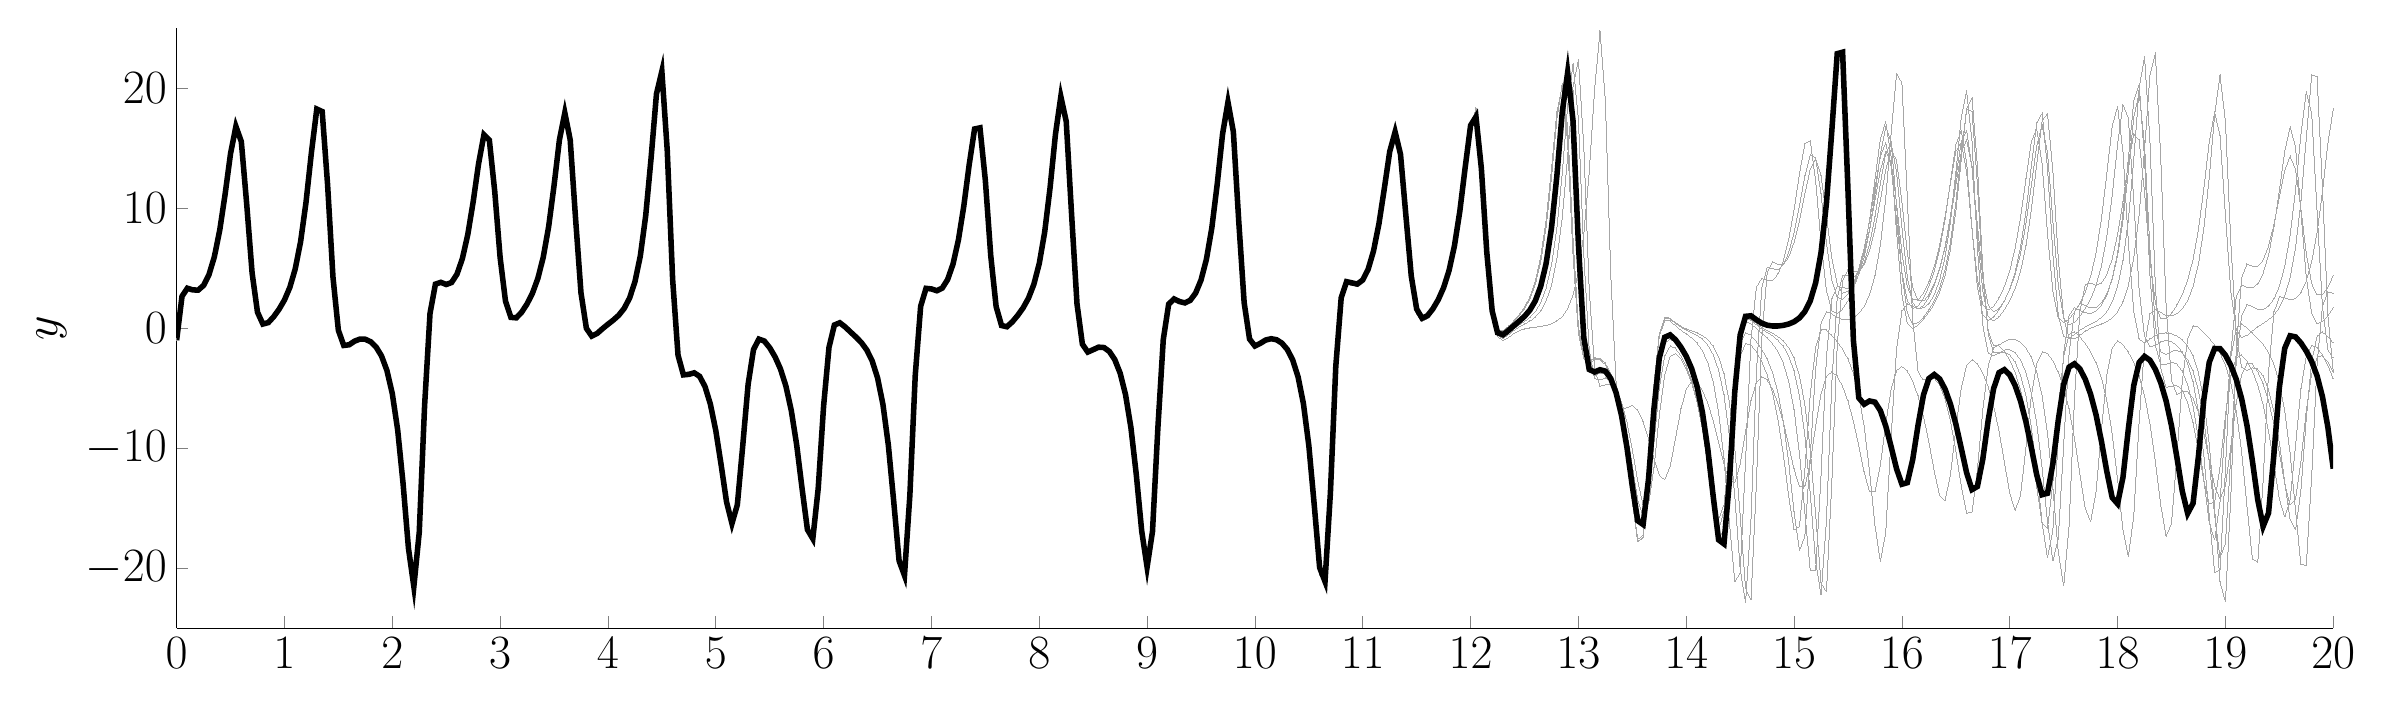
\begin{tikzpicture}

\begin{axis}[%
width=10.783in,
height=3in,
at={(1.809in,1.132in)},
scale only axis,
xmin=0,
xmax=20,
ymin=-25,
ymax=25,
axis background/.style={fill=white},
axis x line*=bottom,
axis y line*=left,
ylabel = {$y$},
ylabel style = {font=\LARGE},
ticklabel style={font=\LARGE},legend style={font=\LARGE},title style={font=\LARGE}
]
\addplot [color=white!65!black,solid,line width=0.0pt,forget plot]
  table[row sep=crcr]{%
0	-1\\
0.05	2.65643\\
0.1	3.33245\\
0.15	3.19178\\
0.2	3.17528\\
0.25	3.56649\\
0.3	4.4601\\
0.35	5.95342\\
0.4	8.1767\\
0.45	11.1781\\
0.5	14.5539\\
0.55	16.8145\\
0.6	15.5538\\
0.65	10.3384\\
0.7	4.60993\\
0.75	1.33387\\
0.8	0.347758\\
0.85	0.467242\\
0.9	0.957197\\
0.95	1.57883\\
1	2.34989\\
1.05	3.40321\\
1.1	4.94145\\
1.15	7.22409\\
1.2	10.4928\\
1.25	14.6308\\
1.3	18.2627\\
1.35	18.0565\\
1.4	11.9744\\
1.45	4.25915\\
1.5	-0.169563\\
1.55	-1.43571\\
1.6	-1.38\\
1.65	-1.08148\\
1.7	-0.904591\\
1.75	-0.919957\\
1.8	-1.13218\\
1.85	-1.56764\\
1.9	-2.30766\\
1.95	-3.51148\\
2	-5.44262\\
2.05	-8.4739\\
2.1	-12.9329\\
2.15	-18.3375\\
2.2	-21.5303\\
2.25	-17.0244\\
2.3	-6.39074\\
2.35	1.23501\\
2.4	3.67462\\
2.45	3.82338\\
2.5	3.64328\\
2.55	3.81077\\
2.6	4.50332\\
2.65	5.79988\\
2.7	7.79407\\
2.75	10.5271\\
2.8	13.6975\\
2.85	16.1235\\
2.9	15.6802\\
2.95	11.4208\\
3	5.89869\\
3.05	2.25001\\
3.1	0.905236\\
3.15	0.862864\\
3.2	1.33711\\
3.25	2.02609\\
3.3	2.91973\\
3.35	4.14791\\
3.4	5.91531\\
3.45	8.45526\\
3.5	11.878\\
3.55	15.6906\\
3.6	17.9515\\
3.65	15.6932\\
3.7	9.10941\\
3.75	2.94714\\
3.8	-0.0076954\\
3.85	-0.659618\\
3.9	-0.433675\\
3.95	-0.0376247\\
4	0.329599\\
4.05	0.67727\\
4.1	1.0805\\
4.15	1.64141\\
4.2	2.49771\\
4.25	3.85205\\
4.3	6.00662\\
4.35	9.35778\\
4.4	14.1612\\
4.45	19.5193\\
4.5	21.4104\\
4.55	14.8243\\
4.6	4.06215\\
4.65	-2.25067\\
4.7	-3.88998\\
4.75	-3.84504\\
4.8	-3.71791\\
4.85	-4.01102\\
4.9	-4.85599\\
4.95	-6.33023\\
5	-8.52061\\
5.05	-11.4044\\
5.1	-14.485\\
5.15	-16.2754\\
5.2	-14.7139\\
5.25	-9.7991\\
5.3	-4.67742\\
5.35	-1.77687\\
5.4	-0.909578\\
5.45	-1.06863\\
5.5	-1.62695\\
5.55	-2.38945\\
5.6	-3.39825\\
5.65	-4.81044\\
5.7	-6.84361\\
5.75	-9.70356\\
5.8	-13.3361\\
5.85	-16.785\\
5.9	-17.5411\\
5.95	-13.3424\\
6	-6.4865\\
6.05	-1.5936\\
6.1	0.266385\\
6.15	0.454197\\
6.2	0.105751\\
6.25	-0.319913\\
6.3	-0.735997\\
6.35	-1.19708\\
6.4	-1.80921\\
6.45	-2.71799\\
6.5	-4.13067\\
6.55	-6.34448\\
6.6	-9.725\\
6.65	-14.4327\\
6.7	-19.3884\\
6.75	-20.5938\\
6.8	-13.8799\\
6.85	-3.88997\\
6.9	1.82948\\
6.95	3.3205\\
7	3.26881\\
7.05	3.12046\\
7.1	3.33901\\
7.15	4.05114\\
7.2	5.3436\\
7.25	7.3457\\
7.3	10.1688\\
7.35	13.6254\\
7.4	16.605\\
7.45	16.7014\\
7.5	12.3158\\
7.55	6.04387\\
7.6	1.79215\\
7.65	0.222244\\
7.7	0.119635\\
7.75	0.525421\\
7.8	1.0642\\
7.85	1.69001\\
7.9	2.49744\\
7.95	3.65208\\
8	5.3836\\
8.05	7.9798\\
8.1	11.6704\\
8.15	16.1273\\
8.2	19.3042\\
8.25	17.2715\\
8.3	9.49015\\
8.35	2.04602\\
8.4	-1.33255\\
8.45	-1.99452\\
8.5	-1.7959\\
8.55	-1.58791\\
8.6	-1.62032\\
8.65	-1.94981\\
8.7	-2.62612\\
8.75	-3.76295\\
8.8	-5.56627\\
8.85	-8.32535\\
8.9	-12.2648\\
8.95	-16.9389\\
9	-19.8932\\
9.05	-16.8551\\
9.1	-8.20773\\
9.15	-0.917382\\
9.2	1.99809\\
9.25	2.42448\\
9.3	2.2032\\
9.35	2.09217\\
9.4	2.30366\\
9.45	2.90357\\
9.5	3.97956\\
9.55	5.69751\\
9.6	8.29234\\
9.65	11.9235\\
9.7	16.1492\\
9.75	18.86\\
9.8	16.479\\
9.85	9.02383\\
9.9	2.17652\\
9.95	-0.912554\\
10	-1.51371\\
10.05	-1.29412\\
10.1	-1.02349\\
10.15	-0.921454\\
10.2	-1.01924\\
10.25	-1.32566\\
10.3	-1.88808\\
10.35	-2.81927\\
10.4	-4.32189\\
10.45	-6.71084\\
10.5	-10.3726\\
10.55	-15.4091\\
10.6	-20.3636\\
10.65	-20.5138\\
10.7	-12.2589\\
10.75	-2.18345\\
10.8	2.75633\\
10.85	3.78473\\
10.9	3.63898\\
10.95	3.57335\\
11	3.95717\\
11.05	4.89527\\
11.1	6.47344\\
11.15	8.79016\\
11.2	11.8092\\
11.25	14.9472\\
11.3	16.5341\\
11.35	14.4543\\
11.4	9.11688\\
11.45	4.02093\\
11.5	1.35992\\
11.55	0.670912\\
11.6	0.901985\\
11.65	1.46588\\
11.7	2.20064\\
11.75	3.16296\\
11.8	4.51492\\
11.85	6.48148\\
11.9	9.29652\\
11.95	12.9871\\
12	16.7459\\
12.05	18.0935\\
12.1	14.2643\\
12.15	7.06271\\
12.2	1.60553\\
12.25	-0.553714\\
12.3	-0.83498\\
12.35	-0.527038\\
12.4	-0.168238\\
12.45	0.118599\\
12.5	0.358348\\
12.55	0.61261\\
12.6	0.953005\\
12.65	1.46917\\
12.7	2.2919\\
12.75	3.62721\\
12.8	5.7972\\
12.85	9.24831\\
12.9	14.3297\\
12.95	20.2007\\
13	22.434\\
13.05	15.1184\\
13.1	3.25904\\
13.15	-3.31087\\
13.2	-4.82451\\
13.25	-4.71256\\
13.3	-4.63387\\
13.35	-5.06408\\
13.4	-6.10723\\
13.45	-7.79453\\
13.5	-10.0927\\
13.55	-12.705\\
13.6	-14.7259\\
13.65	-14.6396\\
13.7	-11.6406\\
13.75	-7.2449\\
13.8	-3.86652\\
13.85	-2.32385\\
13.9	-2.09289\\
13.95	-2.54068\\
14	-3.36244\\
14.05	-4.52141\\
14.1	-6.12116\\
14.15	-8.301\\
14.2	-11.0838\\
14.25	-14.0493\\
14.3	-15.8785\\
14.35	-14.6703\\
14.4	-10.2196\\
14.45	-5.27064\\
14.5	-2.27265\\
14.55	-1.27445\\
14.6	-1.36996\\
14.65	-1.93026\\
14.7	-2.74098\\
14.75	-3.83339\\
14.8	-5.35914\\
14.85	-7.52038\\
14.9	-10.4632\\
14.95	-13.9684\\
15	-16.8061\\
15.05	-16.4897\\
15.1	-11.7172\\
15.15	-5.48421\\
15.2	-1.51104\\
15.25	-0.143714\\
15.3	-0.123454\\
15.35	-0.549844\\
15.4	-1.09095\\
15.45	-1.72005\\
15.5	-2.53909\\
15.55	-3.71779\\
15.6	-5.49036\\
15.65	-8.14827\\
15.7	-11.9126\\
15.75	-16.3986\\
15.8	-19.4179\\
15.85	-16.9943\\
15.9	-8.98447\\
15.95	-1.69568\\
16	1.4748\\
16.05	2.04369\\
16.1	1.83047\\
16.15	1.64027\\
16.2	1.70422\\
16.25	2.07724\\
16.3	2.81542\\
16.35	4.04321\\
16.4	5.97821\\
16.45	8.90919\\
16.5	13.0005\\
16.55	17.5739\\
16.6	19.7739\\
16.65	15.5927\\
16.7	6.79736\\
16.75	0.285804\\
16.8	-2.05283\\
16.85	-2.2885\\
16.9	-2.04987\\
16.95	-1.96272\\
17	-2.1941\\
17.05	-2.80145\\
17.1	-3.87548\\
17.15	-5.5889\\
17.2	-8.18868\\
17.25	-11.8583\\
17.3	-16.1934\\
17.35	-19.0831\\
17.4	-16.7818\\
17.45	-9.13706\\
17.5	-2.0533\\
17.55	1.1262\\
17.6	1.73755\\
17.65	1.5249\\
17.7	1.28594\\
17.75	1.25058\\
17.8	1.46157\\
17.85	1.94833\\
17.9	2.79292\\
17.95	4.16074\\
18	6.31948\\
18.05	9.60902\\
18.1	14.177\\
18.15	19.0106\\
18.2	20.3601\\
18.25	14.1476\\
18.3	4.44088\\
18.35	-1.38274\\
18.4	-3.00858\\
18.45	-2.99812\\
18.5	-2.82039\\
18.55	-2.96302\\
18.6	-3.55796\\
18.65	-4.68843\\
18.7	-6.48892\\
18.75	-9.12359\\
18.8	-12.5885\\
18.85	-16.1557\\
18.9	-17.6312\\
18.95	-14.4331\\
19	-7.80784\\
19.05	-2.38648\\
19.1	-0.0315511\\
19.15	0.374455\\
19.2	0.0741112\\
19.25	-0.368783\\
19.3	-0.821219\\
19.35	-1.32633\\
19.4	-1.99341\\
19.45	-2.97686\\
19.5	-4.49449\\
19.55	-6.84948\\
19.6	-10.3843\\
19.65	-15.1319\\
19.7	-19.668\\
19.75	-19.7531\\
19.8	-12.2869\\
19.85	-2.95748\\
19.9	1.89344\\
19.95	3.03217\\
20	2.91886\\
};
\addplot [color=white!65!black,solid,line width=0.0pt,forget plot]
  table[row sep=crcr]{%
0	-1\\
0.05	2.65643\\
0.1	3.33245\\
0.15	3.19178\\
0.2	3.17528\\
0.25	3.56649\\
0.3	4.4601\\
0.35	5.95343\\
0.4	8.17671\\
0.45	11.1781\\
0.5	14.554\\
0.55	16.8145\\
0.6	15.5538\\
0.65	10.3384\\
0.7	4.60992\\
0.75	1.33387\\
0.8	0.347761\\
0.85	0.467246\\
0.9	0.957203\\
0.95	1.57884\\
1	2.3499\\
1.05	3.40323\\
1.1	4.94147\\
1.15	7.22412\\
1.2	10.4928\\
1.25	14.6309\\
1.3	18.2627\\
1.35	18.0565\\
1.4	11.9743\\
1.45	4.25909\\
1.5	-0.169577\\
1.55	-1.4357\\
1.6	-1.37998\\
1.65	-1.08147\\
1.7	-0.904575\\
1.75	-0.919939\\
1.8	-1.13216\\
1.85	-1.56761\\
1.9	-2.30762\\
1.95	-3.51141\\
2	-5.44251\\
2.05	-8.47375\\
2.1	-12.9327\\
2.15	-18.3373\\
2.2	-21.5304\\
2.25	-17.0247\\
2.3	-6.39112\\
2.35	1.23488\\
2.4	3.67462\\
2.45	3.82342\\
2.5	3.64332\\
2.55	3.81079\\
2.6	4.50332\\
2.65	5.79988\\
2.7	7.79405\\
2.75	10.527\\
2.8	13.6974\\
2.85	16.1234\\
2.9	15.6802\\
2.95	11.4209\\
3	5.89877\\
3.05	2.25008\\
3.1	0.905291\\
3.15	0.862909\\
3.2	1.33716\\
3.25	2.02614\\
3.3	2.9198\\
3.35	4.14799\\
3.4	5.91541\\
3.45	8.45539\\
3.5	11.8781\\
3.55	15.6907\\
3.6	17.9514\\
3.65	15.6929\\
3.7	9.10915\\
3.75	2.94704\\
3.8	-0.00766896\\
3.85	-0.659541\\
3.9	-0.433587\\
3.95	-0.0375244\\
4	0.329721\\
4.05	0.677432\\
4.1	1.08073\\
4.15	1.64174\\
4.2	2.49821\\
4.25	3.85282\\
4.3	6.00778\\
4.35	9.35947\\
4.4	14.1633\\
4.45	19.521\\
4.5	21.4093\\
4.55	14.82\\
4.6	4.05859\\
4.65	-2.25173\\
4.7	-3.88984\\
4.75	-3.84466\\
4.8	-3.71762\\
4.85	-4.0109\\
4.9	-4.85603\\
4.95	-6.33044\\
5	-8.52103\\
5.05	-11.405\\
5.1	-14.4858\\
5.15	-16.2759\\
5.2	-14.7136\\
5.25	-9.79802\\
5.3	-4.67631\\
5.35	-1.77612\\
5.4	-0.909133\\
5.45	-1.06831\\
5.5	-1.62664\\
5.55	-2.3891\\
5.6	-3.39782\\
5.65	-4.8099\\
5.7	-6.84296\\
5.75	-9.70284\\
5.8	-13.3355\\
5.85	-16.785\\
5.9	-17.5422\\
5.95	-13.3441\\
6	-6.48745\\
6.05	-1.59358\\
6.1	0.266904\\
6.15	0.454876\\
6.2	0.106505\\
6.25	-0.319032\\
6.3	-0.734878\\
6.35	-1.19555\\
6.4	-1.80703\\
6.45	-2.71479\\
6.5	-4.12589\\
6.55	-6.33738\\
6.6	-9.71494\\
6.65	-14.4206\\
6.7	-19.3803\\
6.75	-20.6022\\
6.8	-13.9047\\
6.85	-3.90888\\
6.9	1.82417\\
6.95	3.3217\\
7	3.27132\\
7.05	3.12257\\
7.1	3.34043\\
7.15	4.05194\\
7.2	5.34377\\
7.25	7.34507\\
7.3	10.167\\
7.35	13.6222\\
7.4	16.6012\\
7.45	16.6995\\
7.5	12.3182\\
7.55	6.04902\\
7.6	1.79688\\
7.65	0.22573\\
7.7	0.122451\\
7.75	0.528258\\
7.8	1.06759\\
7.85	1.69441\\
7.9	2.50341\\
7.95	3.66037\\
8	5.39519\\
8.05	7.99558\\
8.1	11.6898\\
8.15	16.1444\\
8.2	19.3033\\
8.25	17.24\\
8.3	9.45037\\
8.35	2.02696\\
8.4	-1.33321\\
8.45	-1.98823\\
8.5	-1.78827\\
8.55	-1.58016\\
8.6	-1.61192\\
8.65	-1.93968\\
8.7	-2.61284\\
8.75	-3.74473\\
8.8	-5.54088\\
8.85	-8.29092\\
8.9	-12.2231\\
8.95	-16.9047\\
9	-19.9032\\
9.05	-16.9307\\
9.1	-8.28946\\
9.15	-0.949364\\
9.2	2.00207\\
9.25	2.4401\\
9.3	2.22035\\
9.35	2.10926\\
9.4	2.32205\\
9.45	2.92547\\
9.5	4.00748\\
9.55	5.734\\
9.6	8.3387\\
9.65	11.9753\\
9.7	16.1858\\
9.75	18.8386\\
9.8	16.3813\\
9.85	8.92268\\
9.9	2.1392\\
9.95	-0.901549\\
10	-1.48535\\
10.05	-1.26161\\
10.1	-0.988113\\
10.15	-0.879629\\
10.2	-0.965048\\
10.25	-1.25064\\
10.3	-1.77968\\
10.35	-2.65826\\
10.4	-4.0794\\
10.45	-6.34805\\
10.5	-9.85722\\
10.55	-14.7949\\
10.6	-19.9966\\
10.65	-21.0516\\
10.7	-13.5506\\
10.75	-3.04924\\
10.8	2.56225\\
10.85	3.86951\\
10.9	3.76454\\
10.95	3.66878\\
11	4.01254\\
11.05	4.91192\\
11.1	6.44738\\
11.15	8.70905\\
11.2	11.6602\\
11.25	14.7464\\
11.3	16.3773\\
11.35	14.4912\\
11.4	9.35624\\
11.45	4.29857\\
11.5	1.57006\\
11.55	0.819581\\
11.6	1.02675\\
11.65	1.59662\\
11.7	2.35768\\
11.75	3.36313\\
11.8	4.77513\\
11.85	6.81572\\
11.9	9.69772\\
11.95	13.3759\\
12	16.89\\
12.05	17.6766\\
12.1	13.3972\\
12.15	6.41103\\
12.2	1.46039\\
12.25	-0.397567\\
12.3	-0.576756\\
12.35	-0.234251\\
12.4	0.16679\\
12.45	0.536696\\
12.5	0.922796\\
12.55	1.41711\\
12.6	2.14198\\
12.65	3.27006\\
12.7	5.05783\\
12.75	7.86512\\
12.8	12.0511\\
12.85	17.3715\\
12.9	21.2928\\
12.95	18.3903\\
13	8.28549\\
13.05	-0.238426\\
13.1	-3.39858\\
13.15	-3.7663\\
13.2	-3.56959\\
13.25	-3.64502\\
13.3	-4.21852\\
13.35	-5.37362\\
13.4	-7.20583\\
13.45	-9.79468\\
13.5	-12.9736\\
13.55	-15.8181\\
13.6	-16.2924\\
13.65	-12.7847\\
13.7	-7.09034\\
13.75	-2.77393\\
13.8	-0.939735\\
13.85	-0.680412\\
13.9	-1.06986\\
13.95	-1.69668\\
14	-2.4962\\
14.05	-3.57034\\
14.1	-5.1066\\
14.15	-7.34363\\
14.2	-10.4845\\
14.25	-14.3678\\
14.3	-17.6727\\
14.35	-17.4221\\
14.4	-11.8939\\
14.45	-4.78549\\
14.5	-0.522054\\
14.55	0.796439\\
14.6	0.770796\\
14.65	0.414663\\
14.7	0.0819351\\
14.75	-0.175929\\
14.8	-0.402082\\
14.85	-0.659904\\
14.9	-1.02149\\
14.95	-1.58108\\
15	-2.48069\\
15.05	-3.94639\\
15.1	-6.32894\\
15.15	-10.0936\\
15.2	-15.4998\\
15.25	-21.2171\\
15.3	-21.9391\\
15.35	-12.7886\\
15.4	-1.34667\\
15.45	3.98604\\
15.5	4.94757\\
15.55	4.7607\\
15.6	4.76818\\
15.65	5.32552\\
15.7	6.50651\\
15.75	8.32787\\
15.8	10.7098\\
15.85	13.2368\\
15.9	14.8396\\
15.95	14.0464\\
16	10.5652\\
16.05	6.33029\\
16.1	3.44574\\
16.15	2.29612\\
16.2	2.27313\\
16.25	2.82966\\
16.3	3.74204\\
16.35	5.01668\\
16.4	6.77005\\
16.45	9.11754\\
16.5	11.9809\\
16.55	14.7077\\
16.6	15.7305\\
16.65	13.4408\\
16.7	8.6128\\
16.75	4.22886\\
16.8	1.95466\\
16.85	1.38317\\
16.9	1.66551\\
16.95	2.32577\\
17	3.24562\\
17.05	4.50305\\
17.1	6.26909\\
17.15	8.72952\\
17.2	11.9131\\
17.25	15.2507\\
17.3	16.9591\\
17.35	14.7042\\
17.4	8.95857\\
17.45	3.60338\\
17.5	0.916914\\
17.55	0.271948\\
17.6	0.515585\\
17.65	1.0378\\
17.7	1.67425\\
17.75	2.47484\\
17.8	3.58736\\
17.85	5.22609\\
17.9	7.65911\\
17.95	11.1107\\
18	15.3462\\
18.05	18.6713\\
18.1	17.5299\\
18.15	10.6746\\
18.2	3.20675\\
18.25	-0.622998\\
18.3	-1.55796\\
18.35	-1.41367\\
18.4	-1.13183\\
18.45	-1.00729\\
18.5	-1.09284\\
18.55	-1.39977\\
18.6	-1.97392\\
18.65	-2.92717\\
18.7	-4.46207\\
18.75	-6.89097\\
18.8	-10.5848\\
18.85	-15.5906\\
18.9	-20.3361\\
18.95	-20.104\\
19	-11.7612\\
19.05	-2.03607\\
19.1	2.63462\\
19.15	3.58685\\
19.2	3.43423\\
19.25	3.3644\\
19.3	3.72803\\
19.35	4.62779\\
19.4	6.15524\\
19.45	8.42884\\
19.5	11.4664\\
19.55	14.7898\\
19.6	16.8059\\
19.65	15.1656\\
19.7	9.79401\\
19.75	4.26527\\
19.8	1.24536\\
19.85	0.398076\\
19.9	0.569185\\
19.95	1.08185\\
20	1.73017\\
};
\addplot [color=white!65!black,solid,line width=0.0pt,forget plot]
  table[row sep=crcr]{%
0	-1\\
0.05	2.65643\\
0.1	3.33245\\
0.15	3.19178\\
0.2	3.17528\\
0.25	3.56649\\
0.3	4.4601\\
0.35	5.95342\\
0.4	8.17671\\
0.45	11.1781\\
0.5	14.5539\\
0.55	16.8145\\
0.6	15.5538\\
0.65	10.3384\\
0.7	4.60993\\
0.75	1.33387\\
0.8	0.347756\\
0.85	0.467242\\
0.9	0.957199\\
0.95	1.57883\\
1	2.3499\\
1.05	3.40322\\
1.1	4.94146\\
1.15	7.2241\\
1.2	10.4928\\
1.25	14.6309\\
1.3	18.2627\\
1.35	18.0565\\
1.4	11.9744\\
1.45	4.25913\\
1.5	-0.169565\\
1.55	-1.43571\\
1.6	-1.37999\\
1.65	-1.08147\\
1.7	-0.904578\\
1.75	-0.919944\\
1.8	-1.13216\\
1.85	-1.56762\\
1.9	-2.30762\\
1.95	-3.51142\\
2	-5.44253\\
2.05	-8.47377\\
2.1	-12.9327\\
2.15	-18.3373\\
2.2	-21.5304\\
2.25	-17.0247\\
2.3	-6.39107\\
2.35	1.23489\\
2.4	3.67462\\
2.45	3.82342\\
2.5	3.64332\\
2.55	3.81079\\
2.6	4.50333\\
2.65	5.79988\\
2.7	7.79405\\
2.75	10.527\\
2.8	13.6974\\
2.85	16.1234\\
2.9	15.6802\\
2.95	11.4208\\
3	5.89876\\
3.05	2.25007\\
3.1	0.905286\\
3.15	0.862906\\
3.2	1.33715\\
3.25	2.02613\\
3.3	2.91979\\
3.35	4.14798\\
3.4	5.9154\\
3.45	8.45537\\
3.5	11.8781\\
3.55	15.6907\\
3.6	17.9514\\
3.65	15.693\\
3.7	9.10918\\
3.75	2.94705\\
3.8	-0.00767127\\
3.85	-0.659548\\
3.9	-0.433593\\
3.95	-0.0375335\\
4	0.329711\\
4.05	0.677418\\
4.1	1.08071\\
4.15	1.64171\\
4.2	2.49817\\
4.25	3.85275\\
4.3	6.00768\\
4.35	9.35933\\
4.4	14.1632\\
4.45	19.5208\\
4.5	21.4094\\
4.55	14.8204\\
4.6	4.05889\\
4.65	-2.25164\\
4.7	-3.88985\\
4.75	-3.84469\\
4.8	-3.71764\\
4.85	-4.0109\\
4.9	-4.85602\\
4.95	-6.33041\\
5	-8.52099\\
5.05	-11.405\\
5.1	-14.4857\\
5.15	-16.2758\\
5.2	-14.7136\\
5.25	-9.79813\\
5.3	-4.6764\\
5.35	-1.77618\\
5.4	-0.909158\\
5.45	-1.06832\\
5.5	-1.62665\\
5.55	-2.38911\\
5.6	-3.39783\\
5.65	-4.80991\\
5.7	-6.84297\\
5.75	-9.70285\\
5.8	-13.3355\\
5.85	-16.785\\
5.9	-17.5421\\
5.95	-13.344\\
6	-6.48747\\
6.05	-1.5936\\
6.1	0.266878\\
6.15	0.454854\\
6.2	0.106482\\
6.25	-0.319059\\
6.3	-0.734914\\
6.35	-1.19561\\
6.4	-1.8071\\
6.45	-2.7149\\
6.5	-4.12605\\
6.55	-6.33762\\
6.6	-9.71528\\
6.65	-14.421\\
6.7	-19.3805\\
6.75	-20.6019\\
6.8	-13.9038\\
6.85	-3.90824\\
6.9	1.82434\\
6.95	3.32165\\
7	3.27123\\
7.05	3.12248\\
7.1	3.34037\\
7.15	4.0519\\
7.2	5.34375\\
7.25	7.34507\\
7.3	10.167\\
7.35	13.6223\\
7.4	16.6013\\
7.45	16.6996\\
7.5	12.3182\\
7.55	6.04889\\
7.6	1.79673\\
7.65	0.225597\\
7.7	0.122333\\
7.75	0.528137\\
7.8	1.06744\\
7.85	1.69422\\
7.9	2.50315\\
7.95	3.66001\\
8	5.39469\\
8.05	7.99489\\
8.1	11.689\\
8.15	16.1436\\
8.2	19.3033\\
8.25	17.2414\\
8.3	9.45212\\
8.35	2.02782\\
8.4	-1.33316\\
8.45	-1.98848\\
8.5	-1.78858\\
8.55	-1.58047\\
8.6	-1.61226\\
8.65	-1.94009\\
8.7	-2.61337\\
8.75	-3.74544\\
8.8	-5.54187\\
8.85	-8.29226\\
8.9	-12.2248\\
8.95	-16.906\\
9	-19.9028\\
9.05	-16.9278\\
9.1	-8.28629\\
9.15	-0.948142\\
9.2	2.00189\\
9.25	2.43947\\
9.3	2.21966\\
9.35	2.10857\\
9.4	2.3213\\
9.45	2.92457\\
9.5	4.00633\\
9.55	5.73249\\
9.6	8.33679\\
9.65	11.9732\\
9.7	16.1843\\
9.75	18.8395\\
9.8	16.3853\\
9.85	8.92686\\
9.9	2.14076\\
9.95	-0.901974\\
10	-1.48649\\
10.05	-1.26293\\
10.1	-0.989545\\
10.15	-0.881321\\
10.2	-0.967237\\
10.25	-1.25367\\
10.3	-1.78406\\
10.35	-2.66477\\
10.4	-4.08922\\
10.45	-6.36279\\
10.5	-9.87831\\
10.55	-14.8205\\
10.6	-20.0133\\
10.65	-21.0318\\
10.7	-13.4971\\
10.75	-3.01133\\
10.8	2.57148\\
10.85	3.8663\\
10.9	3.75936\\
10.95	3.66482\\
11	4.01029\\
11.05	4.91133\\
11.1	6.44862\\
11.15	8.71262\\
11.2	11.6666\\
11.25	14.7549\\
11.3	16.3838\\
11.35	14.4894\\
11.4	9.346\\
11.45	4.2868\\
11.5	1.56125\\
11.55	0.813465\\
11.6	1.02172\\
11.65	1.59142\\
11.7	2.35149\\
11.75	3.3553\\
11.8	4.76505\\
11.85	6.80293\\
11.9	9.68269\\
11.95	13.362\\
12	16.8863\\
12.05	17.6942\\
12.1	13.4297\\
12.15	6.43374\\
12.2	1.46425\\
12.25	-0.404384\\
12.3	-0.587137\\
12.35	-0.245974\\
12.4	0.153251\\
12.45	0.519646\\
12.5	0.899656\\
12.55	1.38406\\
12.6	2.09317\\
12.65	3.19646\\
12.7	4.94616\\
12.75	7.69912\\
12.8	11.8245\\
12.85	17.1379\\
12.9	21.2542\\
12.95	18.7604\\
13	8.78004\\
13.05	-0.00759856\\
13.1	-3.37557\\
13.15	-3.80651\\
13.2	-3.60995\\
13.25	-3.66989\\
13.3	-4.22644\\
13.35	-5.36417\\
13.4	-7.17583\\
13.45	-9.73916\\
13.5	-12.8929\\
13.55	-15.7358\\
13.6	-16.268\\
13.65	-12.862\\
13.7	-7.2207\\
13.75	-2.88182\\
13.8	-1.00764\\
13.85	-0.725042\\
13.9	-1.10819\\
13.95	-1.73887\\
14	-2.54831\\
14.05	-3.63718\\
14.1	-5.19278\\
14.15	-7.45164\\
14.2	-10.6067\\
14.25	-14.4672\\
14.3	-17.6636\\
14.35	-17.2316\\
14.4	-11.6312\\
14.45	-4.64747\\
14.5	-0.527421\\
14.55	0.724937\\
14.6	0.679642\\
14.65	0.313522\\
14.7	-0.0370348\\
14.75	-0.328875\\
14.8	-0.612845\\
14.85	-0.964396\\
14.9	-1.47618\\
14.95	-2.27661\\
15	-3.56195\\
15.05	-5.63507\\
15.1	-8.91588\\
15.15	-13.752\\
15.2	-19.4699\\
15.25	-22.1756\\
15.3	-16.0073\\
15.35	-4.49731\\
15.4	2.56222\\
15.45	4.42677\\
15.5	4.39808\\
15.55	4.27306\\
15.6	4.60463\\
15.65	5.52563\\
15.7	7.09126\\
15.75	9.32843\\
15.8	12.079\\
15.85	14.6329\\
15.9	15.4487\\
15.95	13.0864\\
16	8.42775\\
16.05	4.28217\\
16.1	2.14482\\
16.15	1.62091\\
16.2	1.92511\\
16.25	2.61889\\
16.3	3.59853\\
16.35	4.94627\\
16.4	6.82744\\
16.45	9.39459\\
16.5	12.5727\\
16.55	15.5802\\
16.6	16.4844\\
16.65	13.4262\\
16.7	7.74835\\
16.75	3.11517\\
16.8	1.00822\\
16.85	0.61992\\
16.9	0.961677\\
16.95	1.56201\\
17	2.32525\\
17.05	3.33817\\
17.1	4.77874\\
17.15	6.88232\\
17.2	9.8757\\
17.25	13.7084\\
17.3	17.3268\\
17.35	17.9346\\
17.4	13.1474\\
17.45	5.82115\\
17.5	0.92096\\
17.55	-0.786397\\
17.6	-0.890955\\
17.65	-0.557841\\
17.7	-0.229102\\
17.75	0.00959937\\
17.8	0.188078\\
17.85	0.358326\\
17.9	0.573372\\
17.95	0.893512\\
18	1.40307\\
18.05	2.23527\\
18.1	3.60818\\
18.15	5.8699\\
18.2	9.51048\\
18.25	14.9145\\
18.3	21.097\\
18.35	22.9624\\
18.4	14.3149\\
18.45	1.86385\\
18.5	-4.30887\\
18.55	-5.48907\\
18.6	-5.29896\\
18.65	-5.27735\\
18.7	-5.82016\\
18.75	-6.98741\\
18.8	-8.75266\\
18.85	-10.9636\\
18.9	-13.1273\\
18.95	-14.2152\\
19	-13.0886\\
19.05	-9.84051\\
19.1	-6.22081\\
19.15	-3.83201\\
19.2	-2.91025\\
19.25	-2.97327\\
19.3	-3.59766\\
19.35	-4.61454\\
19.4	-6.03618\\
19.45	-7.94188\\
19.5	-10.3361\\
19.55	-12.9052\\
19.6	-14.6974\\
19.65	-14.2595\\
19.7	-11.0677\\
19.75	-6.82184\\
19.8	-3.73609\\
19.85	-2.40398\\
19.9	-2.27774\\
19.95	-2.782\\
20	-3.65776\\
};
\addplot [color=white!65!black,solid,line width=0.0pt,forget plot]
  table[row sep=crcr]{%
0	-1\\
0.05	2.65643\\
0.1	3.33245\\
0.15	3.19178\\
0.2	3.17528\\
0.25	3.56648\\
0.3	4.4601\\
0.35	5.95342\\
0.4	8.1767\\
0.45	11.1781\\
0.5	14.5539\\
0.55	16.8145\\
0.6	15.5538\\
0.65	10.3384\\
0.7	4.60993\\
0.75	1.33386\\
0.8	0.347753\\
0.85	0.467238\\
0.9	0.957196\\
0.95	1.57883\\
1	2.34989\\
1.05	3.4032\\
1.1	4.94144\\
1.15	7.22407\\
1.2	10.4928\\
1.25	14.6308\\
1.3	18.2627\\
1.35	18.0565\\
1.4	11.9745\\
1.45	4.25918\\
1.5	-0.169556\\
1.55	-1.43572\\
1.6	-1.38001\\
1.65	-1.0815\\
1.7	-0.904603\\
1.75	-0.919973\\
1.8	-1.1322\\
1.85	-1.56767\\
1.9	-2.30771\\
1.95	-3.51155\\
2	-5.44273\\
2.05	-8.47407\\
2.1	-12.9331\\
2.15	-18.3377\\
2.2	-21.5303\\
2.25	-17.0239\\
2.3	-6.3903\\
2.35	1.23518\\
2.4	3.67462\\
2.45	3.82334\\
2.5	3.64325\\
2.55	3.81075\\
2.6	4.50331\\
2.65	5.79989\\
2.7	7.7941\\
2.75	10.5271\\
2.8	13.6976\\
2.85	16.1235\\
2.9	15.6802\\
2.95	11.4207\\
3	5.89857\\
3.05	2.24992\\
3.1	0.905181\\
3.15	0.86283\\
3.2	1.33708\\
3.25	2.02605\\
3.3	2.91969\\
3.35	4.14786\\
3.4	5.91524\\
3.45	8.45518\\
3.5	11.8779\\
3.55	15.6905\\
3.6	17.9515\\
3.65	15.6934\\
3.7	9.10957\\
3.75	2.94719\\
3.8	-0.00772758\\
3.85	-0.659681\\
3.9	-0.433748\\
3.95	-0.0377055\\
4	0.329502\\
4.05	0.677142\\
4.1	1.08032\\
4.15	1.64114\\
4.2	2.49732\\
4.25	3.85145\\
4.3	6.0057\\
4.35	9.35644\\
4.4	14.1595\\
4.45	19.518\\
4.5	21.4113\\
4.55	14.8278\\
4.6	4.06495\\
4.65	-2.24983\\
4.7	-3.8901\\
4.75	-3.84533\\
4.8	-3.71813\\
4.85	-4.01112\\
4.9	-4.85596\\
4.95	-6.33005\\
5	-8.52027\\
5.05	-11.4038\\
5.1	-14.4844\\
5.15	-16.275\\
5.2	-14.7142\\
5.25	-9.79998\\
5.3	-4.67833\\
5.35	-1.77747\\
5.4	-0.909926\\
5.45	-1.06887\\
5.5	-1.62717\\
5.55	-2.38971\\
5.6	-3.39857\\
5.65	-4.81083\\
5.7	-6.84409\\
5.75	-9.70409\\
5.8	-13.3365\\
5.85	-16.785\\
5.9	-17.5403\\
5.95	-13.3413\\
6	-6.48583\\
6.05	-1.59364\\
6.1	0.265973\\
6.15	0.453673\\
6.2	0.105171\\
6.25	-0.320591\\
6.3	-0.736861\\
6.35	-1.19826\\
6.4	-1.81089\\
6.45	-2.72046\\
6.5	-4.13435\\
6.55	-6.34994\\
6.6	-9.73272\\
6.65	-14.4421\\
6.7	-19.3946\\
6.75	-20.5873\\
6.8	-13.8609\\
6.85	-3.87551\\
6.9	1.83352\\
6.95	3.31956\\
7	3.26688\\
7.05	3.11884\\
7.1	3.33792\\
7.15	4.05052\\
7.2	5.34345\\
7.25	7.34616\\
7.3	10.1701\\
7.35	13.6278\\
7.4	16.608\\
7.45	16.7029\\
7.5	12.314\\
7.55	6.03997\\
7.6	1.78854\\
7.65	0.219572\\
7.7	0.117467\\
7.75	0.523235\\
7.8	1.0616\\
7.85	1.68662\\
7.9	2.49284\\
7.95	3.64569\\
8	5.37467\\
8.05	7.96763\\
8.1	11.6554\\
8.15	16.1141\\
8.2	19.3049\\
8.25	17.2957\\
8.3	9.5209\\
8.35	2.06083\\
8.4	-1.33198\\
8.45	-1.99936\\
8.5	-1.80177\\
8.55	-1.59387\\
8.6	-1.62676\\
8.65	-1.95757\\
8.7	-2.63627\\
8.75	-3.77688\\
8.8	-5.58566\\
8.85	-8.35162\\
8.9	-12.2965\\
8.95	-16.9646\\
9	-19.885\\
9.05	-16.7972\\
9.1	-8.14586\\
9.15	-0.893451\\
9.2	1.99485\\
9.25	2.41249\\
9.3	2.19006\\
9.35	2.07905\\
9.4	2.2895\\
9.45	2.88665\\
9.5	3.95793\\
9.55	5.66917\\
9.6	8.25618\\
9.65	11.8828\\
9.7	16.1198\\
9.75	18.8755\\
9.8	16.5549\\
9.85	9.10367\\
9.9	2.20671\\
9.95	-0.920539\\
10	-1.53548\\
10.05	-1.31916\\
10.1	-1.05068\\
10.15	-0.953483\\
10.2	-1.06064\\
10.25	-1.38286\\
10.3	-1.97059\\
10.35	-2.94156\\
10.4	-4.50546\\
10.45	-6.98376\\
10.5	-10.7548\\
10.55	-15.8475\\
10.6	-20.5788\\
10.65	-20.0457\\
10.7	-11.3274\\
10.75	-1.61862\\
10.8	2.86205\\
10.85	3.71391\\
10.9	3.54679\\
10.95	3.50356\\
11	3.91472\\
11.05	4.87871\\
11.1	6.48568\\
11.15	8.84055\\
11.2	11.9086\\
11.25	15.0874\\
11.3	16.65\\
11.35	14.4381\\
11.4	8.95686\\
11.45	3.82891\\
11.5	1.21007\\
11.55	0.560504\\
11.6	0.80572\\
11.65	1.36265\\
11.7	2.07494\\
11.75	3.00071\\
11.8	4.30071\\
11.85	6.20028\\
11.9	8.94696\\
11.95	12.6227\\
12	16.5523\\
12.05	18.3722\\
12.1	15.0113\\
12.15	7.70495\\
12.2	1.80181\\
12.25	-0.649833\\
12.3	-1.03362\\
12.35	-0.755081\\
12.4	-0.424189\\
12.45	-0.194386\\
12.5	-0.0586875\\
12.55	0.0222662\\
12.6	0.0824859\\
12.65	0.146984\\
12.7	0.237556\\
12.75	0.380407\\
12.8	0.615202\\
12.85	1.00782\\
12.9	1.67079\\
12.95	2.79682\\
13	4.70987\\
13.05	7.91768\\
13.1	13.0303\\
13.15	19.9238\\
13.2	24.8027\\
13.25	19.0066\\
13.3	4.44811\\
13.35	-4.6479\\
13.4	-6.76683\\
13.45	-6.60866\\
13.5	-6.43357\\
13.55	-6.80463\\
13.6	-7.76062\\
13.65	-9.18808\\
13.7	-10.8368\\
13.75	-12.2182\\
13.8	-12.615\\
13.85	-11.4965\\
13.9	-9.17171\\
13.95	-6.72332\\
14	-5.06236\\
14.05	-4.39302\\
14.1	-4.50093\\
14.15	-5.1489\\
14.2	-6.21596\\
14.25	-7.66349\\
14.3	-9.43213\\
14.35	-11.2942\\
14.4	-12.7027\\
14.45	-12.8531\\
14.5	-11.2763\\
14.55	-8.56623\\
14.6	-6.02536\\
14.65	-4.49717\\
14.7	-4.015\\
14.75	-4.27753\\
14.8	-5.04411\\
14.85	-6.22042\\
14.9	-7.79368\\
14.95	-9.71355\\
15	-11.7223\\
15.05	-13.1775\\
15.1	-13.1486\\
15.15	-11.1797\\
15.2	-8.11007\\
15.25	-5.4473\\
15.3	-3.98632\\
15.35	-3.62142\\
15.4	-3.9797\\
15.45	-4.81553\\
15.5	-6.05637\\
15.55	-7.71757\\
15.6	-9.77462\\
15.65	-11.9747\\
15.7	-13.6142\\
15.75	-13.6091\\
15.8	-11.3916\\
15.85	-7.94733\\
15.9	-5.03779\\
15.95	-3.51091\\
16	-3.1655\\
16.05	-3.54983\\
16.1	-4.39359\\
16.15	-5.63291\\
16.2	-7.3121\\
16.25	-9.45752\\
16.3	-11.8855\\
16.35	-13.9226\\
16.4	-14.3308\\
16.45	-12.1858\\
16.5	-8.35025\\
16.55	-4.93497\\
16.6	-3.09182\\
16.65	-2.61217\\
16.7	-2.93163\\
16.75	-3.70621\\
16.8	-4.84967\\
16.85	-6.42405\\
16.9	-8.52376\\
16.95	-11.1136\\
17	-13.7318\\
17.05	-15.1636\\
17.1	-13.879\\
17.15	-9.91164\\
17.2	-5.58674\\
17.25	-2.90933\\
17.3	-1.97971\\
17.35	-2.08425\\
17.4	-2.69549\\
17.45	-3.62942\\
17.5	-4.92112\\
17.55	-6.70757\\
17.6	-9.12388\\
17.65	-12.1086\\
17.7	-14.9915\\
17.75	-16.0895\\
17.8	-13.631\\
17.85	-8.47399\\
17.9	-3.88644\\
17.95	-1.58637\\
18	-1.04592\\
18.05	-1.33883\\
18.1	-1.9699\\
18.15	-2.82034\\
18.2	-3.96932\\
18.25	-5.59319\\
18.3	-7.9077\\
18.35	-11.0465\\
18.4	-14.688\\
18.45	-17.3259\\
18.5	-16.2414\\
18.55	-10.6633\\
18.6	-4.38458\\
18.65	-0.835465\\
18.7	0.201709\\
18.75	0.093679\\
18.8	-0.33764\\
18.85	-0.823188\\
18.9	-1.35836\\
18.95	-2.04124\\
19	-3.02402\\
19.05	-4.51937\\
19.1	-6.8173\\
19.15	-10.2386\\
19.2	-14.8075\\
19.25	-19.2003\\
19.3	-19.4944\\
19.35	-12.6301\\
19.4	-3.60296\\
19.45	1.3617\\
19.5	2.63856\\
19.55	2.56109\\
19.6	2.37479\\
19.65	2.48252\\
19.7	2.99173\\
19.75	3.97887\\
19.8	5.5827\\
19.85	8.00801\\
19.9	11.4036\\
19.95	15.4177\\
20	18.2704\\
};
\addplot [color=white!65!black,solid,line width=0.0pt,forget plot]
  table[row sep=crcr]{%
0	-1\\
0.05	2.65643\\
0.1	3.33245\\
0.15	3.19178\\
0.2	3.17529\\
0.25	3.56649\\
0.3	4.4601\\
0.35	5.95343\\
0.4	8.17672\\
0.45	11.1781\\
0.5	14.554\\
0.55	16.8145\\
0.6	15.5538\\
0.65	10.3384\\
0.7	4.60991\\
0.75	1.33386\\
0.8	0.347759\\
0.85	0.467246\\
0.9	0.957203\\
0.95	1.57883\\
1	2.3499\\
1.05	3.40322\\
1.1	4.94147\\
1.15	7.22411\\
1.2	10.4928\\
1.25	14.6309\\
1.3	18.2627\\
1.35	18.0565\\
1.4	11.9744\\
1.45	4.2591\\
1.5	-0.169579\\
1.55	-1.43571\\
1.6	-1.37999\\
1.65	-1.08148\\
1.7	-0.904584\\
1.75	-0.919952\\
1.8	-1.13217\\
1.85	-1.56763\\
1.9	-2.30765\\
1.95	-3.51147\\
2	-5.4426\\
2.05	-8.47388\\
2.1	-12.9328\\
2.15	-18.3374\\
2.2	-21.5303\\
2.25	-17.0244\\
2.3	-6.39078\\
2.35	1.23501\\
2.4	3.67463\\
2.45	3.8234\\
2.5	3.6433\\
2.55	3.81079\\
2.6	4.50333\\
2.65	5.7999\\
2.7	7.79409\\
2.75	10.5271\\
2.8	13.6975\\
2.85	16.1234\\
2.9	15.6801\\
2.95	11.4208\\
3	5.89866\\
3.05	2.25001\\
3.1	0.905256\\
3.15	0.862889\\
3.2	1.33714\\
3.25	2.02612\\
3.3	2.91977\\
3.35	4.14796\\
3.4	5.91538\\
3.45	8.45535\\
3.5	11.8781\\
3.55	15.6907\\
3.6	17.9514\\
3.65	15.693\\
3.7	9.10921\\
3.75	2.94704\\
3.8	-0.0077032\\
3.85	-0.659589\\
3.9	-0.433637\\
3.95	-0.0375823\\
4	0.32965\\
4.05	0.677335\\
4.1	1.08059\\
4.15	1.64154\\
4.2	2.49792\\
4.25	3.85237\\
4.3	6.0071\\
4.35	9.35848\\
4.4	14.1621\\
4.45	19.52\\
4.5	21.4099\\
4.55	14.8225\\
4.6	4.06066\\
4.65	-2.25112\\
4.7	-3.88994\\
4.75	-3.84489\\
4.8	-3.7178\\
4.85	-4.01098\\
4.9	-4.85602\\
4.95	-6.33033\\
5	-8.52081\\
5.05	-11.4047\\
5.1	-14.4853\\
5.15	-16.2755\\
5.2	-14.7138\\
5.25	-9.79862\\
5.3	-4.67695\\
5.35	-1.77657\\
5.4	-0.909405\\
5.45	-1.06851\\
5.5	-1.62684\\
5.55	-2.38932\\
5.6	-3.3981\\
5.65	-4.81025\\
5.7	-6.84339\\
5.75	-9.70332\\
5.8	-13.3359\\
5.85	-16.7851\\
5.9	-17.5415\\
5.95	-13.343\\
6	-6.4868\\
6.05	-1.59355\\
6.1	0.266594\\
6.15	0.45446\\
6.2	0.10604\\
6.25	-0.319573\\
6.3	-0.735566\\
6.35	-1.19649\\
6.4	-1.80837\\
6.45	-2.71676\\
6.5	-4.12883\\
6.55	-6.34175\\
6.6	-9.72113\\
6.65	-14.4281\\
6.7	-19.3853\\
6.75	-20.5971\\
6.8	-13.8894\\
6.85	-3.89723\\
6.9	1.82745\\
6.95	3.32097\\
7	3.26979\\
7.05	3.12128\\
7.1	3.33957\\
7.15	4.05146\\
7.2	5.34369\\
7.25	7.34549\\
7.3	10.1681\\
7.35	13.6242\\
7.4	16.6036\\
7.45	16.7006\\
7.5	12.3167\\
7.55	6.0458\\
7.6	1.79396\\
7.65	0.223595\\
7.7	0.120737\\
7.75	0.526534\\
7.8	1.06553\\
7.85	1.69173\\
7.9	2.49978\\
7.95	3.65533\\
8	5.38815\\
8.05	7.98599\\
8.1	11.678\\
8.15	16.134\\
8.2	19.3039\\
8.25	17.2592\\
8.3	9.47452\\
8.35	2.0385\\
8.4	-1.33283\\
8.45	-1.99207\\
8.5	-1.79292\\
8.55	-1.58489\\
8.6	-1.61705\\
8.65	-1.94588\\
8.7	-2.62096\\
8.75	-3.75588\\
8.8	-5.55643\\
8.85	-8.31201\\
8.9	-12.2487\\
8.95	-16.9257\\
9	-19.8972\\
9.05	-16.8844\\
9.1	-8.23928\\
9.15	-0.929656\\
9.2	1.99969\\
9.25	2.43056\\
9.3	2.20987\\
9.35	2.09883\\
9.4	2.31084\\
9.45	2.91213\\
9.5	3.99048\\
9.55	5.71181\\
9.6	8.31054\\
9.65	11.9439\\
9.7	16.1637\\
9.75	18.8518\\
9.8	16.4407\\
9.85	8.98394\\
9.9	2.16166\\
9.95	-0.908365\\
10	-1.50266\\
10.05	-1.28144\\
10.1	-1.0097\\
10.15	-0.905171\\
10.2	-0.998165\\
10.25	-1.29651\\
10.3	-1.84598\\
10.35	-2.75678\\
10.4	-4.22788\\
10.45	-6.57049\\
10.5	-10.1742\\
10.55	-15.1757\\
10.6	-20.2327\\
10.65	-20.7342\\
10.7	-12.7519\\
10.75	-2.502\\
10.8	2.68917\\
10.85	3.81898\\
10.9	3.68715\\
10.95	3.60987\\
11	3.97871\\
11.05	4.90242\\
11.1	6.46469\\
11.15	8.7607\\
11.2	11.7539\\
11.25	14.8715\\
11.3	16.4739\\
11.35	14.4666\\
11.4	9.20587\\
11.45	4.12519\\
11.5	1.43964\\
11.55	0.728119\\
11.6	0.950678\\
11.65	1.51736\\
11.7	2.26279\\
11.75	3.24255\\
11.8	4.61898\\
11.85	6.6162\\
11.9	9.46029\\
11.95	13.15\\
12	16.8157\\
12.05	17.9363\\
12.1	13.9112\\
12.15	6.78535\\
12.2	1.53565\\
12.25	-0.496439\\
12.3	-0.734209\\
12.35	-0.412412\\
12.4	-0.0378913\\
12.45	0.280251\\
12.5	0.575755\\
12.55	0.921955\\
12.6	1.41021\\
12.65	2.16325\\
12.7	3.36489\\
12.75	5.29804\\
12.8	8.36293\\
12.85	12.9372\\
12.9	18.5981\\
12.95	22.0847\\
13	17.4141\\
13.05	6.15371\\
13.1	-1.77653\\
13.15	-4.20017\\
13.2	-4.30643\\
13.25	-4.13961\\
13.3	-4.37458\\
13.35	-5.17885\\
13.4	-6.61643\\
13.45	-8.73752\\
13.5	-11.4637\\
13.55	-14.251\\
13.6	-15.6917\\
13.65	-14.0516\\
13.7	-9.54085\\
13.75	-4.93089\\
13.8	-2.28379\\
13.85	-1.4717\\
13.9	-1.64608\\
13.95	-2.25945\\
14	-3.14286\\
14.05	-4.34818\\
14.1	-6.03362\\
14.15	-8.38395\\
14.2	-11.4587\\
14.25	-14.7995\\
14.3	-16.8167\\
14.35	-15.1606\\
14.4	-9.77128\\
14.45	-4.24026\\
14.5	-1.22776\\
14.55	-0.386688\\
14.6	-0.560199\\
14.65	-1.07252\\
14.7	-1.7188\\
14.75	-2.53272\\
14.8	-3.65702\\
14.85	-5.30311\\
14.9	-7.73266\\
14.95	-11.1546\\
15	-15.3092\\
15.05	-18.5013\\
15.1	-17.2909\\
15.15	-10.5766\\
15.2	-3.30919\\
15.25	0.439265\\
15.3	1.36763\\
15.35	1.22163\\
15.4	0.917225\\
15.45	0.741123\\
15.5	0.737453\\
15.55	0.901221\\
15.6	1.24953\\
15.65	1.84739\\
15.7	2.82699\\
15.75	4.41502\\
15.8	6.95961\\
15.85	10.8823\\
15.9	16.2501\\
15.95	21.2582\\
16	20.4801\\
16.05	10.8809\\
16.1	0.740118\\
16.15	-3.60912\\
16.2	-4.31251\\
16.25	-4.12317\\
16.3	-4.15368\\
16.35	-4.7059\\
16.4	-5.86372\\
16.45	-7.6896\\
16.5	-10.1954\\
16.55	-13.1043\\
16.6	-15.4109\\
16.65	-15.3025\\
16.7	-11.7848\\
16.75	-6.76672\\
16.8	-3.11626\\
16.85	-1.58459\\
16.9	-1.41771\\
16.95	-1.87426\\
17	-2.63113\\
17.05	-3.66004\\
17.1	-5.08287\\
17.15	-7.0873\\
17.2	-9.83203\\
17.25	-13.1958\\
17.3	-16.2168\\
17.35	-16.6747\\
17.4	-12.8168\\
17.45	-6.72592\\
17.5	-2.28463\\
17.55	-0.500224\\
17.6	-0.293951\\
17.65	-0.681576\\
17.7	-1.24814\\
17.75	-1.92962\\
17.8	-2.81943\\
17.85	-4.09047\\
17.9	-5.97936\\
17.95	-8.76029\\
18	-12.571\\
18.05	-16.8003\\
18.1	-18.9885\\
18.15	-15.6096\\
18.2	-7.74461\\
18.25	-1.37594\\
18.3	1.19936\\
18.35	1.58099\\
18.4	1.32481\\
18.45	1.08738\\
18.5	1.04272\\
18.55	1.21556\\
18.6	1.6263\\
18.65	2.3448\\
18.7	3.51737\\
18.75	5.39098\\
18.8	8.31606\\
18.85	12.603\\
18.9	17.8277\\
18.95	21.126\\
19	17.2936\\
19.05	7.2005\\
19.1	-0.554489\\
19.15	-3.24784\\
19.2	-3.49673\\
19.25	-3.30005\\
19.3	-3.387\\
19.35	-3.9546\\
19.4	-5.08627\\
19.45	-6.89135\\
19.5	-9.48308\\
19.55	-12.7648\\
19.6	-15.9034\\
19.65	-16.8142\\
19.7	-13.4933\\
19.75	-7.47608\\
19.8	-2.71512\\
19.85	-0.642501\\
19.9	-0.302111\\
19.95	-0.648547\\
20	-1.20543\\
};
\addplot [color=white!65!black,solid,line width=0.0pt,forget plot]
  table[row sep=crcr]{%
0	-1\\
0.05	2.65643\\
0.1	3.33245\\
0.15	3.19178\\
0.2	3.17528\\
0.25	3.56649\\
0.3	4.4601\\
0.35	5.95343\\
0.4	8.17671\\
0.45	11.1781\\
0.5	14.554\\
0.55	16.8145\\
0.6	15.5538\\
0.65	10.3384\\
0.7	4.60993\\
0.75	1.33387\\
0.8	0.347764\\
0.85	0.467249\\
0.9	0.957208\\
0.95	1.57884\\
1	2.34991\\
1.05	3.40324\\
1.1	4.94148\\
1.15	7.22413\\
1.2	10.4929\\
1.25	14.6309\\
1.3	18.2627\\
1.35	18.0564\\
1.4	11.9743\\
1.45	4.25907\\
1.5	-0.16958\\
1.55	-1.4357\\
1.6	-1.37997\\
1.65	-1.08146\\
1.7	-0.904564\\
1.75	-0.919926\\
1.8	-1.13214\\
1.85	-1.56758\\
1.9	-2.30758\\
1.95	-3.51135\\
2	-5.44243\\
2.05	-8.47362\\
2.1	-12.9325\\
2.15	-18.3371\\
2.2	-21.5304\\
2.25	-17.025\\
2.3	-6.39145\\
2.35	1.23475\\
2.4	3.67463\\
2.45	3.82347\\
2.5	3.64336\\
2.55	3.81082\\
2.6	4.50335\\
2.65	5.79989\\
2.7	7.79405\\
2.75	10.527\\
2.8	13.6974\\
2.85	16.1233\\
2.9	15.6801\\
2.95	11.4209\\
3	5.89884\\
3.05	2.25015\\
3.1	0.905352\\
3.15	0.862962\\
3.2	1.33721\\
3.25	2.0262\\
3.3	2.91987\\
3.35	4.14809\\
3.4	5.91554\\
3.45	8.45556\\
3.5	11.8783\\
3.55	15.6908\\
3.6	17.9513\\
3.65	15.6926\\
3.7	9.10879\\
3.75	2.94689\\
3.8	-0.00764449\\
3.85	-0.659448\\
3.9	-0.433472\\
3.95	-0.0373965\\
4	0.329876\\
4.05	0.677636\\
4.1	1.08101\\
4.15	1.64216\\
4.2	2.49884\\
4.25	3.85377\\
4.3	6.00924\\
4.35	9.3616\\
4.4	14.166\\
4.45	19.5231\\
4.5	21.4079\\
4.55	14.8145\\
4.6	4.05415\\
4.65	-2.25307\\
4.7	-3.88966\\
4.75	-3.84419\\
4.8	-3.71728\\
4.85	-4.01074\\
4.9	-4.85607\\
4.95	-6.3307\\
5	-8.52157\\
5.05	-11.4059\\
5.1	-14.4867\\
5.15	-16.2765\\
5.2	-14.7132\\
5.25	-9.79664\\
5.3	-4.67489\\
5.35	-1.77518\\
5.4	-0.908571\\
5.45	-1.06792\\
5.5	-1.62627\\
5.55	-2.38867\\
5.6	-3.39729\\
5.65	-4.80924\\
5.7	-6.84216\\
5.75	-9.70196\\
5.8	-13.3348\\
5.85	-16.785\\
5.9	-17.5435\\
5.95	-13.346\\
6	-6.48861\\
6.05	-1.59353\\
6.1	0.267569\\
6.15	0.455737\\
6.2	0.107459\\
6.25	-0.31792\\
6.3	-0.733463\\
6.35	-1.19363\\
6.4	-1.80428\\
6.45	-2.71076\\
6.5	-4.11987\\
6.55	-6.32844\\
6.6	-9.70227\\
6.65	-14.4053\\
6.7	-19.37\\
6.75	-20.6127\\
6.8	-13.9358\\
6.85	-3.93272\\
6.9	1.81746\\
6.95	3.32321\\
7	3.27448\\
7.05	3.12521\\
7.1	3.34222\\
7.15	4.05293\\
7.2	5.34398\\
7.25	7.34427\\
7.3	10.1648\\
7.35	13.6182\\
7.4	16.5963\\
7.45	16.697\\
7.5	12.3213\\
7.55	6.05551\\
7.6	1.80284\\
7.65	0.230107\\
7.7	0.125983\\
7.75	0.531814\\
7.8	1.07182\\
7.85	1.69991\\
7.9	2.51087\\
7.95	3.67075\\
8	5.40969\\
8.05	8.01531\\
8.1	11.714\\
8.15	16.1656\\
8.2	19.3018\\
8.25	17.2006\\
8.3	9.40085\\
8.35	2.00336\\
8.4	-1.33393\\
8.45	-1.98033\\
8.5	-1.77871\\
8.55	-1.57043\\
8.6	-1.60138\\
8.65	-1.92695\\
8.7	-2.59613\\
8.75	-3.72175\\
8.8	-5.50882\\
8.85	-8.24735\\
8.9	-12.1702\\
8.95	-16.8608\\
9	-19.9149\\
9.05	-17.026\\
9.1	-8.39391\\
9.15	-0.990852\\
9.2	2.00665\\
9.25	2.4597\\
9.3	2.24193\\
9.35	2.13068\\
9.4	2.345\\
9.45	2.95269\\
9.5	4.04205\\
9.55	5.77902\\
9.6	8.39565\\
9.65	12.0385\\
9.7	16.2293\\
9.75	18.8102\\
9.8	16.2605\\
9.85	8.8004\\
9.9	2.09555\\
9.95	-0.886784\\
10	-1.44979\\
10.05	-1.22101\\
10.1	-0.943788\\
10.15	-0.827008\\
10.2	-0.896633\\
10.25	-1.15571\\
10.3	-1.64221\\
10.35	-2.45357\\
10.4	-3.76991\\
10.45	-5.88152\\
10.5	-9.18313\\
10.55	-13.9544\\
10.6	-19.3861\\
10.65	-21.5723\\
10.7	-15.2785\\
10.75	-4.38313\\
10.8	2.19827\\
10.85	3.95584\\
10.9	3.93137\\
10.95	3.79776\\
11	4.08359\\
11.05	4.92554\\
11.1	6.39839\\
11.15	8.5819\\
11.2	11.4407\\
11.25	14.4627\\
11.3	16.1668\\
11.35	14.5588\\
11.4	9.70699\\
11.45	4.69635\\
11.5	1.86258\\
11.55	1.01647\\
11.6	1.18298\\
11.65	1.75423\\
11.7	2.54274\\
11.75	3.59433\\
11.8	5.06847\\
11.85	7.18008\\
11.9	10.1121\\
11.95	13.7326\\
12	16.9274\\
12.05	17.1211\\
12.1	12.4956\\
12.15	5.84381\\
12.2	1.4129\\
12.25	-0.167354\\
12.3	-0.255222\\
12.35	0.127339\\
12.4	0.58902\\
12.45	1.07349\\
12.5	1.65473\\
12.55	2.4627\\
12.6	3.67937\\
12.65	5.56051\\
12.7	8.43683\\
12.75	12.5648\\
12.8	17.4622\\
12.85	20.4114\\
12.9	16.7918\\
12.95	7.48651\\
13	0.151132\\
13.05	-2.55097\\
13.1	-2.85992\\
13.15	-2.64513\\
13.2	-2.62694\\
13.25	-3.00394\\
13.3	-3.8533\\
13.35	-5.28626\\
13.4	-7.47896\\
13.45	-10.5876\\
13.5	-14.4058\\
13.55	-17.5784\\
13.6	-17.1869\\
13.65	-11.6859\\
13.7	-4.75923\\
13.75	-0.628647\\
13.8	0.647247\\
13.85	0.61141\\
13.9	0.239634\\
13.95	-0.129142\\
14	-0.452489\\
14.05	-0.786232\\
14.1	-1.21574\\
14.15	-1.85045\\
14.2	-2.84555\\
14.25	-4.43678\\
14.3	-6.97214\\
14.35	-10.8655\\
14.4	-16.1735\\
14.45	-21.1116\\
14.5	-20.3684\\
14.55	-10.9563\\
14.6	-0.921912\\
14.65	3.44534\\
14.7	4.17689\\
14.75	3.99175\\
14.8	4.00704\\
14.85	4.5305\\
14.9	5.65016\\
14.95	7.43705\\
15	9.92759\\
15.05	12.9005\\
15.1	15.4247\\
15.15	15.6557\\
15.2	12.3226\\
15.25	7.13683\\
15.3	3.19094\\
15.35	1.46852\\
15.4	1.21933\\
15.45	1.63433\\
15.5	2.34464\\
15.55	3.30027\\
15.6	4.61365\\
15.65	6.47491\\
15.7	9.07838\\
15.75	12.4272\\
15.8	15.825\\
15.85	17.2318\\
15.9	14.2815\\
15.95	8.0631\\
16	2.8257\\
16.05	0.448524\\
16.1	-0.00619056\\
16.15	0.29346\\
16.2	0.793252\\
16.25	1.3625\\
16.3	2.05829\\
16.35	3.01997\\
16.4	4.44817\\
16.45	6.61119\\
16.5	9.80408\\
16.55	14.075\\
16.6	18.3456\\
16.65	19.2454\\
16.7	13.5673\\
16.75	4.95112\\
16.8	-0.406892\\
16.85	-2.03925\\
16.9	-2.06785\\
16.95	-1.82079\\
17	-1.76355\\
17.05	-2.01138\\
17.1	-2.61249\\
17.15	-3.66034\\
17.2	-5.33436\\
17.25	-7.89755\\
17.3	-11.5786\\
17.35	-16.076\\
17.4	-19.38\\
17.45	-17.4941\\
17.5	-9.68189\\
17.55	-2.07532\\
17.6	1.40507\\
17.65	2.09628\\
17.7	1.90435\\
17.75	1.70695\\
17.8	1.76352\\
17.85	2.13627\\
17.9	2.88179\\
17.95	4.12367\\
18	6.07761\\
18.05	9.02579\\
18.1	13.1112\\
18.15	17.6073\\
18.2	19.6253\\
18.25	15.306\\
18.3	6.62129\\
18.35	0.297321\\
18.4	-1.95336\\
18.45	-2.16853\\
18.5	-1.92348\\
18.55	-1.82123\\
18.6	-2.02056\\
18.65	-2.57331\\
18.7	-3.56312\\
18.75	-5.15532\\
18.8	-7.60021\\
18.85	-11.1341\\
18.9	-15.545\\
18.95	-19.0819\\
19	-17.9134\\
19.05	-10.6372\\
19.1	-2.81124\\
19.15	1.07592\\
19.2	1.96781\\
19.25	1.8141\\
19.3	1.58328\\
19.35	1.57452\\
19.4	1.85478\\
19.45	2.46786\\
19.5	3.51486\\
19.55	5.1865\\
19.6	7.76409\\
19.65	11.5111\\
19.7	16.1778\\
19.75	19.7445\\
19.8	17.9439\\
19.85	9.78233\\
19.9	1.79825\\
19.95	-1.79151\\
20	-2.47506\\
};
\addplot [color=white!65!black,solid,line width=0.0pt,forget plot]
  table[row sep=crcr]{%
0	-1\\
0.05	2.65643\\
0.1	3.33245\\
0.15	3.19178\\
0.2	3.17528\\
0.25	3.56649\\
0.3	4.4601\\
0.35	5.95343\\
0.4	8.17671\\
0.45	11.1781\\
0.5	14.554\\
0.55	16.8145\\
0.6	15.5538\\
0.65	10.3384\\
0.7	4.60993\\
0.75	1.33387\\
0.8	0.34776\\
0.85	0.467247\\
0.9	0.957207\\
0.95	1.57884\\
1	2.34991\\
1.05	3.40323\\
1.1	4.94148\\
1.15	7.22412\\
1.2	10.4928\\
1.25	14.6309\\
1.3	18.2627\\
1.35	18.0565\\
1.4	11.9743\\
1.45	4.25909\\
1.5	-0.169569\\
1.55	-1.43569\\
1.6	-1.37997\\
1.65	-1.08146\\
1.7	-0.90456\\
1.75	-0.919922\\
1.8	-1.13213\\
1.85	-1.56757\\
1.9	-2.30756\\
1.95	-3.51132\\
2	-5.44238\\
2.05	-8.47355\\
2.1	-12.9324\\
2.15	-18.3371\\
2.2	-21.5304\\
2.25	-17.0252\\
2.3	-6.39161\\
2.35	1.23469\\
2.4	3.67463\\
2.45	3.82348\\
2.5	3.64338\\
2.55	3.81083\\
2.6	4.50335\\
2.65	5.79988\\
2.7	7.79403\\
2.75	10.527\\
2.8	13.6974\\
2.85	16.1233\\
2.9	15.6801\\
2.95	11.4209\\
3	5.89889\\
3.05	2.25019\\
3.1	0.90537\\
3.15	0.862973\\
3.2	1.33722\\
3.25	2.02621\\
3.3	2.91988\\
3.35	4.1481\\
3.4	5.91556\\
3.45	8.45558\\
3.5	11.8783\\
3.55	15.6908\\
3.6	17.9513\\
3.65	15.6925\\
3.7	9.10875\\
3.75	2.94688\\
3.8	-0.00763145\\
3.85	-0.659428\\
3.9	-0.433449\\
3.95	-0.0373698\\
4	0.329907\\
4.05	0.677673\\
4.1	1.08107\\
4.15	1.64223\\
4.2	2.49895\\
4.25	3.85395\\
4.3	6.00949\\
4.35	9.36197\\
4.4	14.1665\\
4.45	19.5234\\
4.5	21.4076\\
4.55	14.8136\\
4.6	4.05336\\
4.65	-2.2533\\
4.7	-3.88963\\
4.75	-3.84411\\
4.8	-3.71721\\
4.85	-4.01071\\
4.9	-4.85608\\
4.95	-6.33074\\
5	-8.52166\\
5.05	-11.406\\
5.1	-14.4869\\
5.15	-16.2766\\
5.2	-14.7131\\
5.25	-9.79642\\
5.3	-4.67465\\
5.35	-1.77502\\
5.4	-0.908471\\
5.45	-1.06784\\
5.5	-1.62619\\
5.55	-2.38858\\
5.6	-3.39718\\
5.65	-4.8091\\
5.7	-6.84199\\
5.75	-9.70177\\
5.8	-13.3346\\
5.85	-16.785\\
5.9	-17.5437\\
5.95	-13.3465\\
6	-6.48888\\
6.05	-1.59355\\
6.1	0.267687\\
6.15	0.455896\\
6.2	0.107635\\
6.25	-0.317713\\
6.3	-0.733202\\
6.35	-1.19327\\
6.4	-1.80378\\
6.45	-2.71001\\
6.5	-4.11876\\
6.55	-6.3268\\
6.6	-9.69994\\
6.65	-14.4025\\
6.7	-19.3681\\
6.75	-20.6146\\
6.8	-13.9416\\
6.85	-3.93713\\
6.9	1.8162\\
6.95	3.32347\\
7	3.27505\\
7.05	3.12569\\
7.1	3.34253\\
7.15	4.0531\\
7.2	5.344\\
7.25	7.34409\\
7.3	10.1643\\
7.35	13.6174\\
7.4	16.5954\\
7.45	16.6966\\
7.5	12.322\\
7.55	6.05676\\
7.6	1.80396\\
7.65	0.230911\\
7.7	0.12662\\
7.75	0.532451\\
7.8	1.07258\\
7.85	1.7009\\
7.9	2.51222\\
7.95	3.67261\\
8	5.41229\\
8.05	8.01884\\
8.1	11.7183\\
8.15	16.1694\\
8.2	19.3015\\
8.25	17.1935\\
8.3	9.39202\\
8.35	1.99918\\
8.4	-1.33404\\
8.45	-1.9789\\
8.5	-1.77699\\
8.55	-1.56868\\
8.6	-1.59947\\
8.65	-1.92464\\
8.7	-2.5931\\
8.75	-3.71758\\
8.8	-5.503\\
8.85	-8.23943\\
8.9	-12.1605\\
8.95	-16.8528\\
9	-19.9169\\
9.05	-17.0433\\
9.1	-8.41303\\
9.15	-0.998534\\
9.2	2.00742\\
9.25	2.46323\\
9.3	2.24582\\
9.35	2.13454\\
9.4	2.34912\\
9.45	2.95755\\
9.5	4.04822\\
9.55	5.78702\\
9.6	8.40574\\
9.65	12.0496\\
9.7	16.2369\\
9.75	18.8048\\
9.8	16.239\\
9.85	8.77896\\
9.9	2.08809\\
9.95	-0.884001\\
10	-1.44339\\
10.05	-1.21372\\
10.1	-0.935799\\
10.15	-0.817496\\
10.2	-0.884236\\
10.25	-1.13848\\
10.3	-1.61723\\
10.35	-2.41631\\
10.4	-3.71344\\
10.45	-5.79599\\
10.5	-9.05825\\
10.55	-13.7944\\
10.6	-19.257\\
10.65	-21.6438\\
10.7	-15.6002\\
10.75	-4.65748\\
10.8	2.1145\\
10.85	3.96794\\
10.9	3.96259\\
10.95	3.82237\\
11	4.09678\\
11.05	4.92722\\
11.1	6.38761\\
11.15	8.55587\\
11.2	11.397\\
11.25	14.4075\\
11.3	16.1267\\
11.35	14.573\\
11.4	9.77636\\
11.45	4.77463\\
11.5	1.91938\\
11.55	1.05355\\
11.6	1.21123\\
11.65	1.78186\\
11.7	2.57458\\
11.75	3.63347\\
11.8	5.11716\\
11.85	7.23894\\
11.9	10.1761\\
11.95	13.782\\
12	16.9199\\
12.05	17.0211\\
12.1	12.3556\\
12.15	5.7674\\
12.2	1.41729\\
12.25	-0.122736\\
12.3	-0.197583\\
12.35	0.19193\\
12.4	0.665253\\
12.45	1.17125\\
12.5	1.78845\\
12.55	2.65339\\
12.6	3.9576\\
12.65	5.96747\\
12.7	9.01229\\
12.75	13.2855\\
12.8	18.0627\\
12.85	20.2189\\
12.9	15.474\\
12.95	6.13858\\
13	-0.379102\\
13.05	-2.54487\\
13.1	-2.69678\\
13.15	-2.47832\\
13.2	-2.48774\\
13.25	-2.88573\\
13.3	-3.74493\\
13.35	-5.18283\\
13.4	-7.38735\\
13.45	-10.5346\\
13.5	-14.4469\\
13.55	-17.7722\\
13.6	-17.4747\\
13.65	-11.833\\
13.7	-4.65892\\
13.75	-0.407712\\
13.8	0.883756\\
13.85	0.847393\\
13.9	0.497781\\
13.95	0.185797\\
14	-0.0362513\\
14.05	-0.205776\\
14.1	-0.374605\\
14.15	-0.594958\\
14.2	-0.927932\\
14.25	-1.4611\\
14.3	-2.33433\\
14.35	-3.77699\\
14.4	-6.15348\\
14.45	-9.96553\\
14.5	-15.55\\
14.55	-21.6449\\
14.6	-22.6483\\
14.65	-13.0046\\
14.7	-0.864025\\
14.75	4.62787\\
14.8	5.53477\\
14.85	5.31835\\
14.9	5.34641\\
14.95	5.95453\\
15	7.18648\\
15.05	9.00414\\
15.1	11.2255\\
15.15	13.3005\\
15.2	14.1579\\
15.25	12.7474\\
15.3	9.38459\\
15.35	5.89003\\
15.4	3.70346\\
15.45	2.92895\\
15.5	3.07414\\
15.55	3.74986\\
15.6	4.81506\\
15.65	6.29419\\
15.7	8.26188\\
15.75	10.6917\\
15.8	13.1975\\
15.85	14.7373\\
15.9	13.9\\
15.95	10.459\\
16	6.32148\\
16.05	3.51238\\
16.1	2.39493\\
16.15	2.38282\\
16.2	2.94884\\
16.25	3.87777\\
16.3	5.1774\\
16.35	6.95985\\
16.4	9.32579\\
16.45	12.1615\\
16.5	14.7578\\
16.55	15.5344\\
16.6	13.043\\
16.65	8.26826\\
16.7	4.10566\\
16.75	2.00848\\
16.8	1.52142\\
16.85	1.84178\\
16.9	2.53515\\
16.95	3.50415\\
17	4.8356\\
17.05	6.70008\\
17.1	9.26186\\
17.15	12.4724\\
17.2	15.5896\\
17.25	16.6752\\
17.3	13.7227\\
17.35	7.93923\\
17.4	3.1211\\
17.45	0.903653\\
17.5	0.475082\\
17.55	0.798232\\
17.6	1.37242\\
17.65	2.08859\\
17.7	3.02504\\
17.75	4.35175\\
17.8	6.30143\\
17.85	9.12734\\
17.9	12.9003\\
17.95	16.8708\\
18	18.5088\\
18.05	14.7281\\
18.1	7.18438\\
18.15	1.39705\\
18.2	-0.879442\\
18.25	-1.1796\\
18.3	-0.892657\\
18.35	-0.595184\\
18.4	-0.42786\\
18.45	-0.388319\\
18.5	-0.455062\\
18.55	-0.626584\\
18.6	-0.932438\\
18.65	-1.44213\\
18.7	-2.28274\\
18.75	-3.67019\\
18.8	-5.95118\\
18.85	-9.61007\\
18.9	-15.0088\\
18.95	-21.1039\\
19	-22.7703\\
19.05	-14.0509\\
19.1	-1.79683\\
19.15	4.2255\\
19.2	5.37135\\
19.25	5.18374\\
19.3	5.16706\\
19.35	5.71167\\
19.4	6.88159\\
19.45	8.66017\\
19.5	10.911\\
19.55	13.1565\\
19.6	14.356\\
19.65	13.2966\\
19.7	9.99478\\
19.75	6.24424\\
19.8	3.75033\\
19.85	2.77882\\
19.9	2.82206\\
19.95	3.43134\\
20	4.42666\\
};
\addplot [color=white!65!black,solid,line width=0.0pt,forget plot]
  table[row sep=crcr]{%
0	-1\\
0.05	2.65643\\
0.1	3.33245\\
0.15	3.19178\\
0.2	3.17528\\
0.25	3.56648\\
0.3	4.4601\\
0.35	5.95343\\
0.4	8.17671\\
0.45	11.1781\\
0.5	14.554\\
0.55	16.8145\\
0.6	15.5538\\
0.65	10.3384\\
0.7	4.60992\\
0.75	1.33386\\
0.8	0.347756\\
0.85	0.467242\\
0.9	0.9572\\
0.95	1.57883\\
1	2.3499\\
1.05	3.40322\\
1.1	4.94146\\
1.15	7.2241\\
1.2	10.4928\\
1.25	14.6309\\
1.3	18.2627\\
1.35	18.0565\\
1.4	11.9744\\
1.45	4.25912\\
1.5	-0.169571\\
1.55	-1.43571\\
1.6	-1.37999\\
1.65	-1.08148\\
1.7	-0.904584\\
1.75	-0.919951\\
1.8	-1.13217\\
1.85	-1.56763\\
1.9	-2.30765\\
1.95	-3.51145\\
2	-5.44258\\
2.05	-8.47384\\
2.1	-12.9328\\
2.15	-18.3374\\
2.2	-21.5303\\
2.25	-17.0245\\
2.3	-6.39089\\
2.35	1.23497\\
2.4	3.67463\\
2.45	3.82341\\
2.5	3.64331\\
2.55	3.81079\\
2.6	4.50333\\
2.65	5.7999\\
2.7	7.79408\\
2.75	10.5271\\
2.8	13.6975\\
2.85	16.1234\\
2.9	15.6801\\
2.95	11.4208\\
3	5.8987\\
3.05	2.25003\\
3.1	0.905269\\
3.15	0.8629\\
3.2	1.33715\\
3.25	2.02613\\
3.3	2.91979\\
3.35	4.14798\\
3.4	5.9154\\
3.45	8.45538\\
3.5	11.8781\\
3.55	15.6907\\
3.6	17.9514\\
3.65	15.6929\\
3.7	9.10915\\
3.75	2.94703\\
3.8	-0.00768397\\
3.85	-0.659556\\
3.9	-0.433599\\
3.95	-0.0375385\\
4	0.329703\\
4.05	0.677408\\
4.1	1.08069\\
4.15	1.64169\\
4.2	2.49814\\
4.25	3.8527\\
4.3	6.00761\\
4.35	9.35922\\
4.4	14.163\\
4.45	19.5207\\
4.5	21.4094\\
4.55	14.8206\\
4.6	4.05912\\
4.65	-2.25158\\
4.7	-3.88986\\
4.75	-3.84472\\
4.8	-3.71767\\
4.85	-4.01092\\
4.9	-4.85603\\
4.95	-6.33041\\
5	-8.52098\\
5.05	-11.4049\\
5.1	-14.4856\\
5.15	-16.2758\\
5.2	-14.7136\\
5.25	-9.79818\\
5.3	-4.67648\\
5.35	-1.77624\\
5.4	-0.909206\\
5.45	-1.06837\\
5.5	-1.6267\\
5.55	-2.38916\\
5.6	-3.3979\\
5.65	-4.81\\
5.7	-6.84308\\
5.75	-9.70298\\
5.8	-13.3356\\
5.85	-16.785\\
5.9	-17.542\\
5.95	-13.3438\\
6	-6.48727\\
6.05	-1.59356\\
6.1	0.266824\\
6.15	0.454767\\
6.2	0.106383\\
6.25	-0.319176\\
6.3	-0.735058\\
6.35	-1.1958\\
6.4	-1.80738\\
6.45	-2.71531\\
6.5	-4.12667\\
6.55	-6.33854\\
6.6	-9.71658\\
6.65	-14.4226\\
6.7	-19.3816\\
6.75	-20.6009\\
6.8	-13.9006\\
6.85	-3.90578\\
6.9	1.82504\\
6.95	3.32151\\
7	3.27091\\
7.05	3.12222\\
7.1	3.3402\\
7.15	4.05181\\
7.2	5.34375\\
7.25	7.34518\\
7.3	10.1673\\
7.35	13.6227\\
7.4	16.6018\\
7.45	16.6998\\
7.5	12.3178\\
7.55	6.04817\\
7.6	1.79611\\
7.65	0.225166\\
7.7	0.121999\\
7.75	0.527804\\
7.8	1.06704\\
7.85	1.6937\\
7.9	2.50245\\
7.95	3.65904\\
8	5.39333\\
8.05	7.99305\\
8.1	11.6867\\
8.15	16.1417\\
8.2	19.3034\\
8.25	17.2451\\
8.3	9.45674\\
8.35	2.03\\
8.4	-1.33312\\
8.45	-1.98925\\
8.5	-1.7895\\
8.55	-1.58141\\
8.6	-1.61328\\
8.65	-1.94133\\
8.7	-2.61499\\
8.75	-3.74768\\
8.8	-5.545\\
8.85	-8.2965\\
8.9	-12.2299\\
8.95	-16.9103\\
9	-19.9016\\
9.05	-16.9185\\
9.1	-8.27615\\
9.15	-0.944122\\
9.2	2.00144\\
9.25	2.43757\\
9.3	2.21758\\
9.35	2.1065\\
9.4	2.31908\\
9.45	2.92194\\
9.5	4.00299\\
9.55	5.72814\\
9.6	8.33128\\
9.65	11.9671\\
9.7	16.18\\
9.75	18.8422\\
9.8	16.397\\
9.85	8.93878\\
9.9	2.14506\\
9.95	-0.903378\\
10	-1.48993\\
10.05	-1.26686\\
10.1	-0.993831\\
10.15	-0.886401\\
10.2	-0.97383\\
10.25	-1.26281\\
10.3	-1.79727\\
10.35	-2.68442\\
10.4	-4.11885\\
10.45	-6.40724\\
10.5	-9.94185\\
10.55	-14.8975\\
10.6	-20.0629\\
10.65	-20.9711\\
10.7	-13.3361\\
10.75	-2.89835\\
10.8	2.59864\\
10.85	3.85655\\
10.9	3.74381\\
10.95	3.65297\\
11	4.00356\\
11.05	4.9096\\
11.1	6.45239\\
11.15	8.72338\\
11.2	11.6858\\
11.25	14.7803\\
11.3	16.4032\\
11.35	14.4841\\
11.4	9.31512\\
11.45	4.25144\\
11.5	1.53483\\
11.55	0.795126\\
11.6	1.00663\\
11.65	1.5758\\
11.7	2.33286\\
11.75	3.33171\\
11.8	4.73463\\
11.85	6.7643\\
11.9	9.63715\\
11.95	13.3195\\
12	16.8742\\
12.05	17.7466\\
12.1	13.5285\\
12.15	6.50331\\
12.2	1.47656\\
12.25	-0.424714\\
12.3	-0.618373\\
12.35	-0.281251\\
12.4	0.112557\\
12.45	0.468463\\
12.5	0.830237\\
12.55	1.28493\\
12.6	1.94673\\
12.65	2.97543\\
12.7	4.60995\\
12.75	7.19622\\
12.8	11.1269\\
12.85	16.3825\\
12.9	21.0288\\
12.95	19.8107\\
13	10.3785\\
13.05	0.808994\\
13.1	-3.26351\\
13.15	-3.92496\\
13.2	-3.73781\\
13.25	-3.74936\\
13.3	-4.25086\\
13.35	-5.33217\\
13.4	-7.07799\\
13.45	-9.56059\\
13.5	-12.6356\\
13.55	-15.4735\\
13.6	-16.1866\\
13.65	-13.1039\\
13.7	-7.63769\\
13.75	-3.22985\\
13.8	-1.22475\\
13.85	-0.863342\\
13.9	-1.22257\\
13.95	-1.86178\\
14	-2.6979\\
14.05	-3.8264\\
14.1	-5.43251\\
14.15	-7.74473\\
14.2	-10.9248\\
14.25	-14.6992\\
14.3	-17.5789\\
14.35	-16.679\\
14.4	-10.9537\\
14.45	-4.33726\\
14.5	-0.587809\\
14.55	0.502414\\
14.6	0.408419\\
14.65	0.0113379\\
14.7	-0.397058\\
14.75	-0.796189\\
14.8	-1.25993\\
14.85	-1.90026\\
14.9	-2.87006\\
14.95	-4.39076\\
15	-6.78003\\
15.05	-10.4116\\
15.1	-15.3585\\
15.15	-20.1542\\
15.2	-20.2216\\
15.25	-12.188\\
15.3	-2.39029\\
15.35	2.48121\\
15.4	3.52986\\
15.45	3.39218\\
15.5	3.30417\\
15.55	3.63654\\
15.6	4.49589\\
15.65	5.9732\\
15.7	8.19143\\
15.75	11.1935\\
15.8	14.5705\\
15.85	16.8253\\
15.9	15.5477\\
15.95	10.3161\\
16	4.58709\\
16.05	1.31924\\
16.1	0.339513\\
16.15	0.46151\\
16.2	0.951507\\
16.25	1.57188\\
16.3	2.34081\\
16.35	3.3911\\
16.4	4.92525\\
16.45	7.20287\\
16.5	10.4673\\
16.55	14.6076\\
16.6	18.2595\\
16.65	18.0926\\
16.7	12.0303\\
16.75	4.29082\\
16.8	-0.167798\\
16.85	-1.44751\\
16.9	-1.39538\\
16.95	-1.09809\\
17	-0.923487\\
17.05	-0.943647\\
17.1	-1.16425\\
17.15	-1.61334\\
17.2	-2.37494\\
17.25	-3.61245\\
17.3	-5.5946\\
17.35	-8.69594\\
17.4	-13.2229\\
17.45	-18.5956\\
17.5	-21.4665\\
17.55	-16.4735\\
17.6	-5.83999\\
17.65	1.43317\\
17.7	3.66457\\
17.75	3.76267\\
17.8	3.5899\\
17.85	3.77654\\
17.9	4.48815\\
17.95	5.80433\\
18	7.82272\\
18.05	10.587\\
18.1	13.7887\\
18.15	16.2162\\
18.2	15.7039\\
18.25	11.3341\\
18.3	5.7609\\
18.35	2.13368\\
18.4	0.823721\\
18.45	0.799829\\
18.5	1.27597\\
18.55	1.95555\\
18.6	2.83132\\
18.65	4.03353\\
18.7	5.76727\\
18.75	8.27163\\
18.8	11.6804\\
18.85	15.561\\
18.9	18.044\\
18.95	16.0631\\
19	9.49508\\
19.05	3.09947\\
19.1	-0.0457896\\
19.15	-0.773747\\
19.2	-0.57052\\
19.25	-0.191188\\
19.3	0.144027\\
19.35	0.432971\\
19.4	0.738145\\
19.45	1.14126\\
19.5	1.74616\\
19.55	2.7027\\
19.6	4.24221\\
19.65	6.71293\\
19.7	10.5485\\
19.75	15.8882\\
19.8	21.1346\\
19.85	20.9822\\
19.9	11.6962\\
19.95	1.13329\\
20	-3.61213\\
};
\addplot [color=white!65!black,solid,line width=0.0pt,forget plot]
  table[row sep=crcr]{%
0	-1\\
0.05	2.65643\\
0.1	3.33245\\
0.15	3.19178\\
0.2	3.17529\\
0.25	3.56649\\
0.3	4.4601\\
0.35	5.95343\\
0.4	8.17672\\
0.45	11.1781\\
0.5	14.554\\
0.55	16.8145\\
0.6	15.5538\\
0.65	10.3384\\
0.7	4.60991\\
0.75	1.33386\\
0.8	0.34776\\
0.85	0.467249\\
0.9	0.957208\\
0.95	1.57884\\
1	2.34991\\
1.05	3.40323\\
1.1	4.94148\\
1.15	7.22413\\
1.2	10.4928\\
1.25	14.6309\\
1.3	18.2627\\
1.35	18.0564\\
1.4	11.9743\\
1.45	4.25908\\
1.5	-0.169577\\
1.55	-1.43569\\
1.6	-1.37997\\
1.65	-1.08146\\
1.7	-0.904563\\
1.75	-0.919924\\
1.8	-1.13213\\
1.85	-1.56758\\
1.9	-2.30757\\
1.95	-3.51134\\
2	-5.44241\\
2.05	-8.47359\\
2.1	-12.9325\\
2.15	-18.3371\\
2.2	-21.5304\\
2.25	-17.0251\\
2.3	-6.39151\\
2.35	1.23474\\
2.4	3.67464\\
2.45	3.82347\\
2.5	3.64337\\
2.55	3.81083\\
2.6	4.50335\\
2.65	5.79989\\
2.7	7.79404\\
2.75	10.527\\
2.8	13.6974\\
2.85	16.1233\\
2.9	15.6801\\
2.95	11.4209\\
3	5.89885\\
3.05	2.25017\\
3.1	0.905362\\
3.15	0.86297\\
3.2	1.33722\\
3.25	2.02621\\
3.3	2.91988\\
3.35	4.1481\\
3.4	5.91556\\
3.45	8.45558\\
3.5	11.8783\\
3.55	15.6908\\
3.6	17.9513\\
3.65	15.6926\\
3.7	9.10875\\
3.75	2.94687\\
3.8	-0.00763823\\
3.85	-0.659433\\
3.9	-0.433453\\
3.95	-0.0373734\\
4	0.329902\\
4.05	0.677668\\
4.1	1.08106\\
4.15	1.64223\\
4.2	2.49894\\
4.25	3.85392\\
4.3	6.00946\\
4.35	9.36193\\
4.4	14.1665\\
4.45	19.5234\\
4.5	21.4076\\
4.55	14.8137\\
4.6	4.05345\\
4.65	-2.25328\\
4.7	-3.88963\\
4.75	-3.84412\\
4.8	-3.71722\\
4.85	-4.01072\\
4.9	-4.85608\\
4.95	-6.33075\\
5	-8.52166\\
5.05	-11.406\\
5.1	-14.4869\\
5.15	-16.2766\\
5.2	-14.7131\\
5.25	-9.79642\\
5.3	-4.67467\\
5.35	-1.77504\\
5.4	-0.90849\\
5.45	-1.06786\\
5.5	-1.62622\\
5.55	-2.38861\\
5.6	-3.39721\\
5.65	-4.80915\\
5.7	-6.84205\\
5.75	-9.70184\\
5.8	-13.3347\\
5.85	-16.785\\
5.9	-17.5437\\
5.95	-13.3463\\
6	-6.48876\\
6.05	-1.59352\\
6.1	0.267662\\
6.15	0.455856\\
6.2	0.107591\\
6.25	-0.317763\\
6.3	-0.733264\\
6.35	-1.19336\\
6.4	-1.8039\\
6.45	-2.71019\\
6.5	-4.11902\\
6.55	-6.32717\\
6.6	-9.70048\\
6.65	-14.4031\\
6.7	-19.3685\\
6.75	-20.6142\\
6.8	-13.9402\\
6.85	-3.93611\\
6.9	1.8165\\
6.95	3.32342\\
7	3.27492\\
7.05	3.12558\\
7.1	3.34247\\
7.15	4.05307\\
7.2	5.34401\\
7.25	7.34415\\
7.3	10.1644\\
7.35	13.6176\\
7.4	16.5956\\
7.45	16.6967\\
7.5	12.3218\\
7.55	6.05644\\
7.6	1.80368\\
7.65	0.230723\\
7.7	0.126475\\
7.75	0.532308\\
7.8	1.07241\\
7.85	1.70068\\
7.9	2.51191\\
7.95	3.67219\\
8	5.41171\\
8.05	8.01804\\
8.1	11.7174\\
8.15	16.1686\\
8.2	19.3016\\
8.25	17.1951\\
8.3	9.394\\
8.35	2.00011\\
8.4	-1.33402\\
8.45	-1.97923\\
8.5	-1.77739\\
8.55	-1.56909\\
8.6	-1.59992\\
8.65	-1.92519\\
8.7	-2.59382\\
8.75	-3.71857\\
8.8	-5.50438\\
8.85	-8.2413\\
8.9	-12.1628\\
8.95	-16.8547\\
9	-19.9164\\
9.05	-17.0392\\
9.1	-8.40848\\
9.15	-0.996689\\
9.2	2.00726\\
9.25	2.4624\\
9.3	2.24492\\
9.35	2.13365\\
9.4	2.34817\\
9.45	2.95643\\
9.5	4.0468\\
9.55	5.78519\\
9.6	8.40343\\
9.65	12.0471\\
9.7	16.2352\\
9.75	18.8061\\
9.8	16.244\\
9.85	8.78383\\
9.9	2.08975\\
9.95	-0.884673\\
10	-1.44488\\
10.05	-1.21541\\
10.1	-0.937663\\
10.15	-0.819718\\
10.2	-0.887139\\
10.25	-1.14252\\
10.3	-1.62308\\
10.35	-2.42504\\
10.4	-3.72668\\
10.45	-5.81605\\
10.5	-9.08758\\
10.55	-13.8321\\
10.6	-19.2878\\
10.65	-21.6277\\
10.7	-15.5247\\
10.75	-4.59224\\
10.8	2.1347\\
10.85	3.96524\\
10.9	3.95527\\
10.95	3.81659\\
11	4.0937\\
11.05	4.92687\\
11.1	6.39022\\
11.15	8.56208\\
11.2	11.4074\\
11.25	14.4205\\
11.3	16.1361\\
11.35	14.5696\\
11.4	9.7599\\
11.45	4.75609\\
11.5	1.90597\\
11.55	1.04484\\
11.6	1.20464\\
11.65	1.77545\\
11.7	2.56721\\
11.75	3.62443\\
11.8	5.10595\\
11.85	7.22545\\
11.9	10.1615\\
11.95	13.771\\
12	16.922\\
12.05	17.0444\\
12.1	12.3875\\
12.15	5.78446\\
12.2	1.41589\\
12.25	-0.133235\\
12.3	-0.21102\\
12.35	0.176881\\
12.4	0.64747\\
12.45	1.14843\\
12.5	1.75723\\
12.55	2.60889\\
12.6	3.89274\\
12.65	5.87286\\
12.7	8.87932\\
12.75	13.1215\\
12.8	17.9331\\
12.85	20.2792\\
12.9	15.7821\\
12.95	6.43431\\
13	-0.269543\\
13.05	-2.5505\\
13.1	-2.73483\\
13.15	-2.51652\\
13.2	-2.51997\\
13.25	-2.91385\\
13.3	-3.77167\\
13.35	-5.20956\\
13.4	-7.41281\\
13.45	-10.5527\\
13.5	-14.4438\\
13.55	-17.7305\\
13.6	-17.4027\\
13.65	-11.7871\\
13.7	-4.67309\\
13.75	-0.455511\\
13.8	0.829175\\
13.85	0.791924\\
13.9	0.437031\\
13.95	0.111897\\
14	-0.133731\\
14.05	-0.341653\\
14.1	-0.571637\\
14.15	-0.889567\\
14.2	-1.37951\\
14.25	-2.1671\\
14.3	-3.45331\\
14.35	-5.55689\\
14.4	-8.93201\\
14.45	-13.9804\\
14.5	-20.0298\\
14.55	-22.8447\\
14.6	-15.9882\\
14.65	-3.71465\\
14.7	3.38285\\
14.75	5.07527\\
14.8	4.97793\\
14.85	4.88359\\
14.9	5.30413\\
14.95	6.34298\\
15	8.0145\\
15.05	10.2535\\
15.1	12.7201\\
15.15	14.4976\\
15.2	14.1905\\
15.25	11.2196\\
15.3	7.10701\\
15.35	4.00837\\
15.4	2.60722\\
15.45	2.42729\\
15.5	2.9067\\
15.55	3.77713\\
15.6	5.01188\\
15.65	6.7065\\
15.7	8.96415\\
15.75	11.7127\\
15.8	14.3581\\
15.85	15.466\\
15.9	13.4959\\
15.95	8.9934\\
16	4.68823\\
16.05	2.32376\\
16.1	1.65697\\
16.15	1.89539\\
16.2	2.55671\\
16.25	3.50702\\
16.3	4.81302\\
16.35	6.63352\\
16.4	9.12585\\
16.45	12.2494\\
16.5	15.3163\\
16.55	16.5072\\
16.6	13.849\\
16.65	8.30227\\
16.7	3.48291\\
16.75	1.16017\\
16.8	0.656603\\
16.85	0.957483\\
16.9	1.54693\\
16.95	2.30426\\
17	3.30526\\
17.05	4.72232\\
17.1	6.78658\\
17.15	9.72444\\
17.2	13.5037\\
17.25	17.1399\\
17.3	17.9385\\
17.35	13.4293\\
17.4	6.17099\\
17.45	1.14362\\
17.5	-0.678325\\
17.55	-0.828471\\
17.6	-0.497357\\
17.65	-0.14959\\
17.7	0.121542\\
17.75	0.348209\\
17.8	0.591493\\
17.85	0.920572\\
17.9	1.42235\\
17.95	2.22462\\
18	3.52985\\
18.05	5.65678\\
18.1	9.05378\\
18.15	14.098\\
18.2	20.0522\\
18.25	22.6332\\
18.3	15.6511\\
18.35	3.59912\\
18.4	-3.28748\\
18.45	-4.92264\\
18.5	-4.82479\\
18.55	-4.7343\\
18.6	-5.15221\\
18.65	-6.18491\\
18.7	-7.85742\\
18.75	-10.1253\\
18.8	-12.6797\\
18.85	-14.6192\\
18.9	-14.4782\\
18.95	-11.5218\\
19	-7.24275\\
19.05	-3.95691\\
19.1	-2.45041\\
19.15	-2.22742\\
19.2	-2.68155\\
19.25	-3.51893\\
19.3	-4.70462\\
19.35	-6.33843\\
19.4	-8.54654\\
19.45	-11.3178\\
19.5	-14.1683\\
19.55	-15.7316\\
19.6	-14.2316\\
19.65	-9.75288\\
19.7	-5.05109\\
19.75	-2.30064\\
19.8	-1.43068\\
19.85	-1.57975\\
19.9	-2.17745\\
19.95	-3.04128\\
20	-4.21688\\
};
\addplot [color=black,solid,line width=2.0pt,forget plot]
  table[row sep=crcr]{%
0	-1\\
0.05	2.65643\\
0.1	3.33245\\
0.15	3.19178\\
0.2	3.17528\\
0.25	3.56649\\
0.3	4.4601\\
0.35	5.95343\\
0.4	8.17671\\
0.45	11.1781\\
0.5	14.554\\
0.55	16.8145\\
0.6	15.5538\\
0.65	10.3384\\
0.7	4.60992\\
0.75	1.33386\\
0.8	0.347758\\
0.85	0.467245\\
0.9	0.957203\\
0.95	1.57884\\
1	2.3499\\
1.05	3.40322\\
1.1	4.94147\\
1.15	7.22411\\
1.2	10.4928\\
1.25	14.6309\\
1.3	18.2627\\
1.35	18.0565\\
1.4	11.9744\\
1.45	4.25911\\
1.5	-0.169573\\
1.55	-1.4357\\
1.6	-1.37998\\
1.65	-1.08147\\
1.7	-0.904576\\
1.75	-0.919941\\
1.8	-1.13216\\
1.85	-1.56761\\
1.9	-2.30762\\
1.95	-3.51142\\
2	-5.44252\\
2.05	-8.47376\\
2.1	-12.9327\\
2.15	-18.3373\\
2.2	-21.5304\\
2.25	-17.0247\\
2.3	-6.39109\\
2.35	1.23489\\
2.4	3.67463\\
2.45	3.82342\\
2.5	3.64332\\
2.55	3.8108\\
2.6	4.50333\\
2.65	5.79989\\
2.7	7.79406\\
2.75	10.5271\\
2.8	13.6974\\
2.85	16.1234\\
2.9	15.6801\\
2.95	11.4208\\
3	5.89876\\
3.05	2.25008\\
3.1	0.905292\\
3.15	0.862913\\
3.2	1.33716\\
3.25	2.02614\\
3.3	2.9198\\
3.35	4.148\\
3.4	5.91543\\
3.45	8.45541\\
3.5	11.8782\\
3.55	15.6907\\
3.6	17.9514\\
3.65	15.6929\\
3.7	9.1091\\
3.75	2.94701\\
3.8	-0.0076715\\
3.85	-0.659534\\
3.9	-0.433575\\
3.95	-0.0375121\\
4	0.329735\\
4.05	0.67745\\
4.1	1.08075\\
4.15	1.64178\\
4.2	2.49827\\
4.25	3.8529\\
4.3	6.00791\\
4.35	9.35966\\
4.4	14.1636\\
4.45	19.5212\\
4.5	21.4091\\
4.55	14.8195\\
4.6	4.05821\\
4.65	-2.25185\\
4.7	-3.88982\\
4.75	-3.84462\\
4.8	-3.7176\\
4.85	-4.01088\\
4.9	-4.85603\\
4.95	-6.33046\\
5	-8.52108\\
5.05	-11.4051\\
5.1	-14.4858\\
5.15	-16.2759\\
5.2	-14.7136\\
5.25	-9.7979\\
5.3	-4.67618\\
5.35	-1.77604\\
5.4	-0.909082\\
5.45	-1.06827\\
5.5	-1.62661\\
5.55	-2.38906\\
5.6	-3.39777\\
5.65	-4.80984\\
5.7	-6.84288\\
5.75	-9.70276\\
5.8	-13.3354\\
5.85	-16.785\\
5.9	-17.5423\\
5.95	-13.3442\\
6	-6.48757\\
6.05	-1.59358\\
6.1	0.266966\\
6.15	0.454959\\
6.2	0.106597\\
6.25	-0.318925\\
6.3	-0.734742\\
6.35	-1.19537\\
6.4	-1.80677\\
6.45	-2.71441\\
6.5	-4.12532\\
6.55	-6.33654\\
6.6	-9.71374\\
6.65	-14.4192\\
6.7	-19.3793\\
6.75	-20.6032\\
6.8	-13.9076\\
6.85	-3.91112\\
6.9	1.82354\\
6.95	3.32184\\
7	3.27162\\
7.05	3.12281\\
7.1	3.3406\\
7.15	4.05202\\
7.2	5.34379\\
7.25	7.34499\\
7.3	10.1668\\
7.35	13.6218\\
7.4	16.6007\\
7.45	16.6992\\
7.5	12.3186\\
7.55	6.04965\\
7.6	1.79745\\
7.65	0.226138\\
7.7	0.122776\\
7.75	0.528584\\
7.8	1.06797\\
7.85	1.69491\\
7.9	2.50409\\
7.95	3.66132\\
8	5.39652\\
8.05	7.99738\\
8.1	11.692\\
8.15	16.1463\\
8.2	19.3031\\
8.25	17.2364\\
8.3	9.44585\\
8.35	2.02481\\
8.4	-1.33327\\
8.45	-1.9875\\
8.5	-1.78739\\
8.55	-1.57926\\
8.6	-1.61095\\
8.65	-1.93851\\
8.7	-2.6113\\
8.75	-3.74261\\
8.8	-5.53793\\
8.85	-8.2869\\
8.9	-12.2183\\
8.95	-16.9007\\
9	-19.9043\\
9.05	-16.9395\\
9.1	-8.29905\\
9.15	-0.953155\\
9.2	2.00249\\
9.25	2.4419\\
9.3	2.22233\\
9.35	2.11122\\
9.4	2.32416\\
9.45	2.92797\\
9.5	4.01066\\
9.55	5.73814\\
9.6	8.34396\\
9.65	11.9812\\
9.7	16.1899\\
9.75	18.8361\\
9.8	16.3702\\
9.85	8.91132\\
9.9	2.1351\\
9.95	-0.900218\\
10	-1.48208\\
10.05	-1.25788\\
10.1	-0.984043\\
10.15	-0.874804\\
10.2	-0.95878\\
10.25	-1.24195\\
10.3	-1.7671\\
10.35	-2.63956\\
10.4	-4.05118\\
10.45	-6.30567\\
10.5	-9.7965\\
10.55	-14.7208\\
10.6	-19.9476\\
10.65	-21.1073\\
10.7	-13.705\\
10.75	-3.15969\\
10.8	2.53496\\
10.85	3.87853\\
10.9	3.77944\\
10.95	3.68016\\
11	4.01897\\
11.05	4.91348\\
11.1	6.44362\\
11.15	8.69853\\
11.2	11.6415\\
11.25	14.7218\\
11.3	16.3587\\
11.35	14.4965\\
11.4	9.38618\\
11.45	4.33277\\
11.5	1.59553\\
11.55	0.837148\\
11.6	1.0411\\
11.65	1.61141\\
11.7	2.37526\\
11.75	3.38533\\
11.8	4.80367\\
11.85	6.8518\\
11.9	9.73994\\
11.95	13.4146\\
12	16.8995\\
12.05	17.6263\\
12.1	13.3055\\
12.15	6.34805\\
12.2	1.45041\\
12.25	-0.377782\\
12.3	-0.547066\\
12.35	-0.200758\\
12.4	0.205539\\
12.45	0.58556\\
12.5	0.989168\\
12.55	1.51193\\
12.6	2.28196\\
12.65	3.48089\\
12.7	5.37685\\
12.75	8.3363\\
12.8	12.6839\\
12.85	17.9913\\
12.9	21.3096\\
12.95	17.2936\\
13	6.97233\\
13.05	-0.803972\\
13.1	-3.43401\\
13.15	-3.65061\\
13.2	-3.45938\\
13.25	-3.57724\\
13.3	-4.1957\\
13.35	-5.39694\\
13.4	-7.28438\\
13.45	-9.94281\\
13.5	-13.1911\\
13.55	-16.0411\\
13.6	-16.3579\\
13.65	-12.5744\\
13.7	-6.7397\\
13.75	-2.48462\\
13.8	-0.755346\\
13.85	-0.555444\\
13.9	-0.958973\\
13.95	-1.57225\\
14	-2.34072\\
14.05	-3.36853\\
14.1	-4.84253\\
14.15	-7.00567\\
14.2	-10.0884\\
14.25	-14.0169\\
14.3	-17.6335\\
14.35	-17.9714\\
14.4	-12.7543\\
14.45	-5.29456\\
14.5	-0.55774\\
14.55	0.991713\\
14.6	1.03472\\
14.65	0.706429\\
14.7	0.419971\\
14.75	0.253271\\
14.8	0.18496\\
14.85	0.184856\\
14.9	0.238145\\
14.95	0.348523\\
15	0.539057\\
15.05	0.857487\\
15.1	1.38926\\
15.15	2.28196\\
15.2	3.78544\\
15.25	6.30434\\
15.3	10.4039\\
15.35	16.4533\\
15.4	22.8793\\
15.45	23.0004\\
15.5	11.4558\\
15.55	-0.996916\\
15.6	-5.80273\\
15.65	-6.33389\\
15.7	-6.06213\\
15.75	-6.16195\\
15.8	-6.86549\\
15.85	-8.14693\\
15.9	-9.8713\\
15.95	-11.7099\\
16	-13.001\\
16.05	-12.8722\\
16.1	-10.9528\\
16.15	-8.05812\\
16.2	-5.56526\\
16.25	-4.19507\\
16.3	-3.86057\\
16.35	-4.22804\\
16.4	-5.07254\\
16.45	-6.32256\\
16.5	-7.97882\\
16.55	-9.986\\
16.6	-12.0485\\
16.65	-13.4462\\
16.7	-13.1898\\
16.75	-10.9152\\
16.8	-7.67423\\
16.85	-5.04396\\
16.9	-3.70697\\
16.95	-3.45431\\
17	-3.88797\\
17.05	-4.77661\\
17.1	-6.06798\\
17.15	-7.7927\\
17.2	-9.93141\\
17.25	-12.2135\\
17.3	-13.8755\\
17.35	-13.7529\\
17.4	-11.2962\\
17.45	-7.65924\\
17.5	-4.71139\\
17.55	-3.24086\\
17.6	-2.96002\\
17.65	-3.38534\\
17.7	-4.25006\\
17.75	-5.50389\\
17.8	-7.2071\\
17.85	-9.40503\\
17.9	-11.933\\
17.95	-14.1122\\
18	-14.6267\\
18.05	-12.4249\\
18.1	-8.37825\\
18.15	-4.77154\\
18.2	-2.84592\\
18.25	-2.3506\\
18.3	-2.66561\\
18.35	-3.42198\\
18.4	-4.52956\\
18.45	-6.05855\\
18.5	-8.12748\\
18.55	-10.7564\\
18.6	-13.5773\\
18.65	-15.4317\\
18.7	-14.5881\\
18.75	-10.652\\
18.8	-5.9285\\
18.85	-2.84095\\
18.9	-1.69086\\
18.95	-1.70046\\
19	-2.2464\\
19.05	-3.09153\\
19.1	-4.24995\\
19.15	-5.8601\\
19.2	-8.09787\\
19.25	-11.038\\
19.3	-14.3077\\
19.35	-16.5113\\
19.4	-15.397\\
19.45	-10.494\\
19.5	-4.9554\\
19.55	-1.67448\\
19.6	-0.62978\\
19.65	-0.721579\\
19.7	-1.22772\\
19.75	-1.90518\\
19.8	-2.77218\\
19.85	-3.96917\\
19.9	-5.70758\\
19.95	-8.2362\\
20	-11.705\\
};
\end{axis}
\end{tikzpicture}%}
	\end{subfigure}
	\begin{subfigure}{1\linewidth}
		\resizebox{1.0\linewidth}{!}{% This file was created by matlab2tikz.
%
%The latest EFupdates can be retrieved from
%  http://www.mathworks.com/matlabcentral/fileexchange/22022-matlab2tikz-matlab2tikz
%where you can also make suggestions and rate matlab2tikz.
%
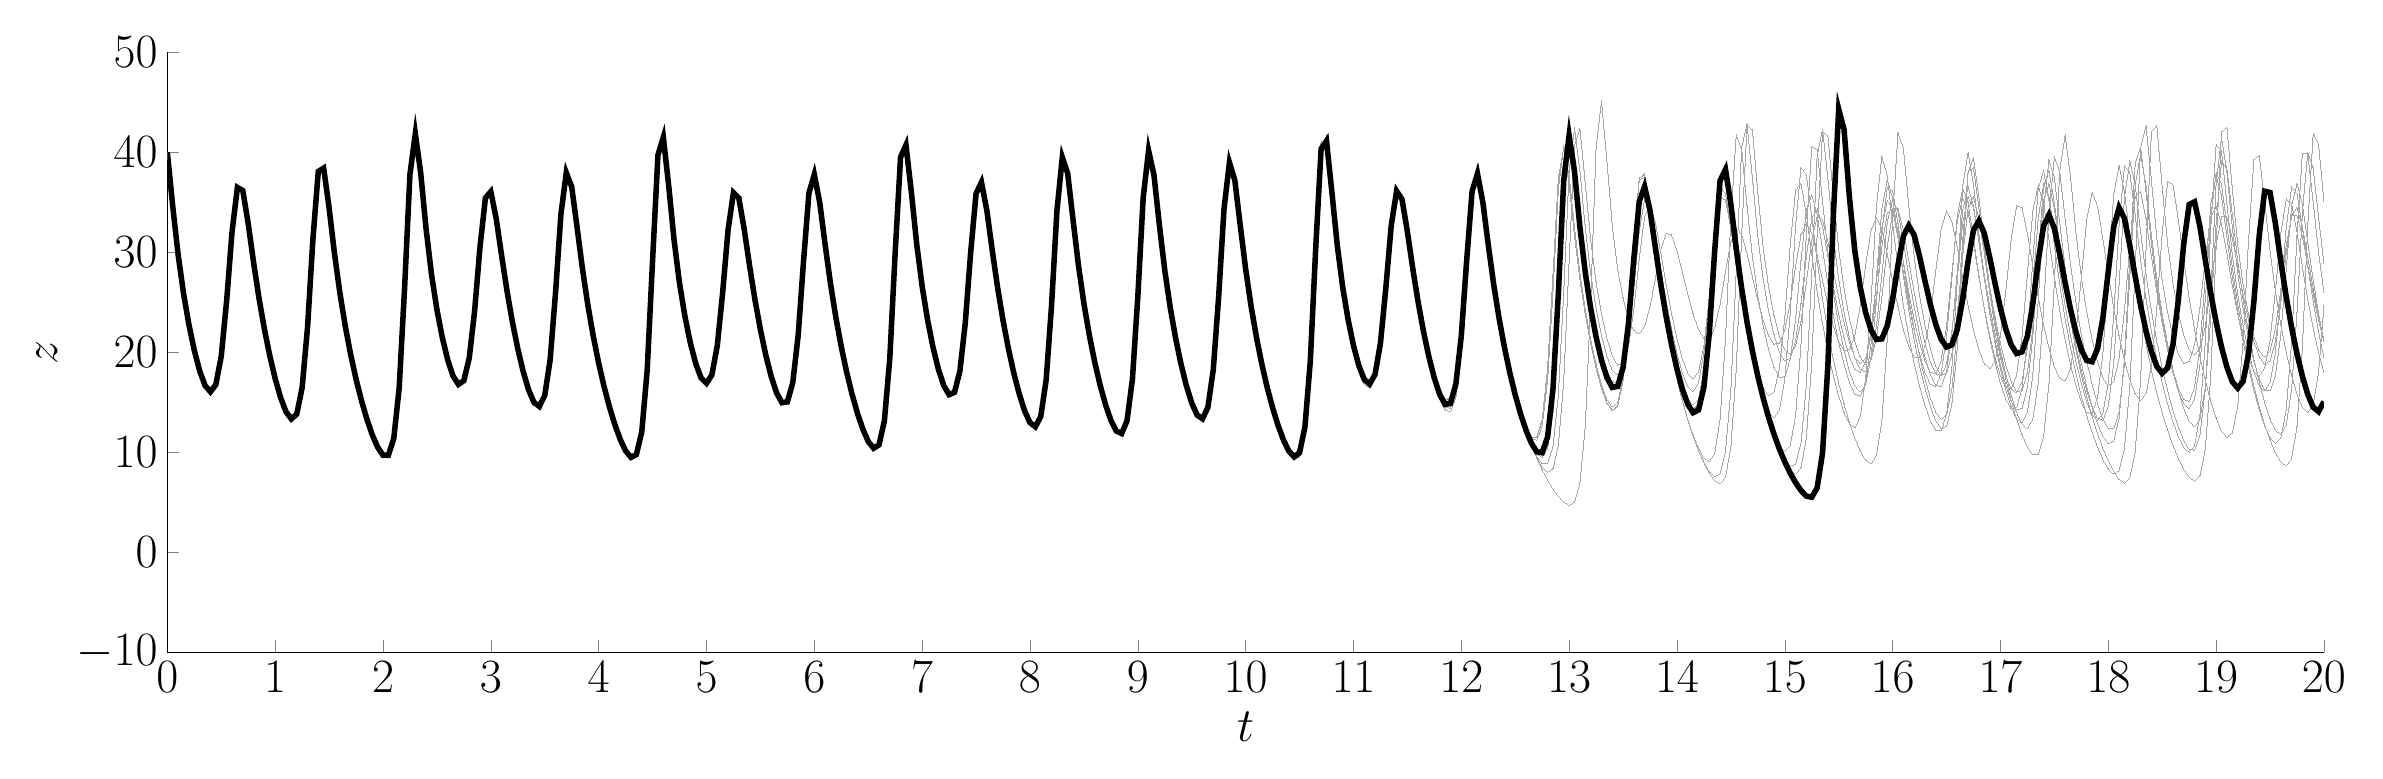
\begin{tikzpicture}

\begin{axis}[%
width=10.783in,
height=3in,
at={(1.809in,1.132in)},
scale only axis,
xmin=0,
xmax=20,
ymin=-10,
ymax=50,
xlabel = {$t$},
xlabel style = {font=\LARGE},
ylabel = {$z$},
ylabel style = {font=\LARGE},
axis background/.style={fill=white},
axis x line*=bottom,
axis y line*=left,
ticklabel style={font=\LARGE},legend style={font=\LARGE},title style={font=\LARGE}
]
\addplot [color=white!65!black,solid,line width=0.0pt,forget plot]
  table[row sep=crcr]{%
0	40\\
0.05	34.6276\\
0.1	29.7744\\
0.15	25.9128\\
0.2	22.7799\\
0.25	20.2007\\
0.3	18.1388\\
0.35	16.6754\\
0.4	16.0515\\
0.45	16.7647\\
0.5	19.599\\
0.55	25.1144\\
0.6	32.0206\\
0.65	36.4888\\
0.7	36.1779\\
0.75	32.8757\\
0.8	28.9825\\
0.85	25.4293\\
0.9	22.338\\
0.95	19.6646\\
1	17.3773\\
1.05	15.4853\\
1.1	14.0664\\
1.15	13.3392\\
1.2	13.8076\\
1.25	16.4436\\
1.3	22.4459\\
1.35	31.2731\\
1.4	38.0812\\
1.45	38.4166\\
1.5	34.4631\\
1.55	29.8993\\
1.6	25.9555\\
1.65	22.6369\\
1.7	19.7928\\
1.75	17.3273\\
1.8	15.1857\\
1.85	13.3362\\
1.9	11.7696\\
1.95	10.5185\\
2	9.71144\\
2.05	9.70621\\
2.1	11.372\\
2.15	16.4042\\
2.2	26.3479\\
2.25	37.797\\
2.3	41.8614\\
2.35	37.9177\\
2.4	32.3252\\
2.45	27.7901\\
2.5	24.2843\\
2.55	21.4819\\
2.6	19.2513\\
2.65	17.6243\\
2.7	16.792\\
2.75	17.1701\\
2.8	19.4336\\
2.85	24.162\\
2.9	30.5556\\
2.95	35.4385\\
3	36.0682\\
3.05	33.3783\\
3.1	29.6825\\
3.15	26.1527\\
3.2	23.0451\\
3.25	20.3595\\
3.3	18.084\\
3.35	16.253\\
3.4	14.9892\\
3.45	14.591\\
3.5	15.6752\\
3.55	19.2328\\
3.6	25.9166\\
3.65	33.7902\\
3.7	37.9594\\
3.75	36.5519\\
3.8	32.5024\\
3.85	28.3395\\
3.9	24.7214\\
3.95	21.6165\\
4	18.9246\\
4.05	16.5794\\
4.1	14.5393\\
4.15	12.7802\\
4.2	11.3013\\
4.25	10.1512\\
4.3	9.49495\\
4.35	9.77744\\
4.4	12.0452\\
4.45	18.1717\\
4.5	29.1506\\
4.55	39.724\\
4.6	41.5063\\
4.65	36.6272\\
4.7	31.1783\\
4.75	26.9148\\
4.8	23.6035\\
4.85	20.9536\\
4.9	18.8773\\
4.95	17.4461\\
5	16.9042\\
5.05	17.7377\\
5.1	20.6454\\
5.15	25.9611\\
5.2	32.2119\\
5.25	35.9548\\
5.3	35.4304\\
5.35	32.3054\\
5.4	28.6326\\
5.45	25.2401\\
5.5	22.2724\\
5.55	19.7214\\
5.6	17.5913\\
5.65	15.9455\\
5.7	14.962\\
5.75	15.0412\\
5.8	16.9417\\
5.85	21.6475\\
5.9	29.0841\\
5.95	35.9265\\
6	37.7726\\
6.05	34.9969\\
6.1	30.8009\\
6.15	26.869\\
6.2	23.4796\\
6.25	20.5553\\
6.3	18.0143\\
6.35	15.807\\
6.4	13.9072\\
6.45	12.3164\\
6.5	11.0905\\
6.55	10.4108\\
6.6	10.7486\\
6.65	13.1644\\
6.7	19.4083\\
6.75	30.0089\\
6.8	39.5325\\
6.85	40.7179\\
6.9	36.0002\\
6.95	30.7742\\
7	26.5865\\
7.05	23.258\\
7.1	20.5357\\
7.15	18.329\\
7.2	16.6755\\
7.25	15.7572\\
7.3	15.9886\\
7.35	18.1089\\
7.4	22.9309\\
7.45	29.9843\\
7.5	35.8736\\
7.55	37.0099\\
7.6	34.1906\\
7.65	30.2071\\
7.7	26.4574\\
7.75	23.1919\\
7.8	20.3652\\
7.85	17.9234\\
7.9	15.846\\
7.95	14.1566\\
8	12.9616\\
8.05	12.5455\\
8.1	13.5552\\
8.15	17.1843\\
8.2	24.6025\\
8.25	34.1078\\
8.3	39.4923\\
8.35	37.8957\\
8.4	33.222\\
8.45	28.6838\\
8.5	24.9125\\
8.55	21.7565\\
8.6	19.0615\\
8.65	16.7505\\
8.7	14.7971\\
8.75	13.2263\\
8.8	12.1556\\
8.85	11.9037\\
8.9	13.2021\\
8.95	17.3888\\
9	25.6325\\
9.05	35.5309\\
9.1	40.1685\\
9.15	37.661\\
9.2	32.683\\
9.25	28.1658\\
9.3	24.482\\
9.35	21.4194\\
9.4	18.8272\\
9.45	16.6485\\
9.5	14.8972\\
9.55	13.6832\\
9.6	13.3029\\
9.65	14.4112\\
9.7	18.1484\\
9.75	25.448\\
9.8	34.3226\\
9.85	38.9923\\
9.9	37.266\\
9.95	32.7839\\
10	28.3978\\
10.05	24.6958\\
10.1	21.5631\\
10.15	18.8646\\
10.2	16.5224\\
10.25	14.4918\\
10.3	12.7498\\
10.35	11.3029\\
10.4	10.2182\\
10.45	9.70736\\
10.5	10.3195\\
10.55	13.2822\\
10.6	20.5086\\
10.65	31.9984\\
10.7	40.8738\\
10.75	40.5425\\
10.8	35.2229\\
10.85	30.0554\\
10.9	26.0434\\
10.95	22.8815\\
11	20.3317\\
11.05	18.341\\
11.1	17.0036\\
11.15	16.5938\\
11.2	17.6455\\
11.25	20.9034\\
11.3	26.6261\\
11.35	33.006\\
11.4	36.3725\\
11.45	35.3453\\
11.5	31.9585\\
11.55	28.2187\\
11.6	24.8281\\
11.65	21.875\\
11.7	19.3343\\
11.75	17.2015\\
11.8	15.5286\\
11.85	14.4749\\
11.9	14.4139\\
11.95	16.0899\\
12	20.5778\\
12.05	28.1377\\
12.1	35.7004\\
12.15	38.2782\\
12.2	35.6721\\
12.25	31.3456\\
12.3	27.2753\\
12.35	23.7929\\
12.4	20.8026\\
12.45	18.205\\
12.5	15.9376\\
12.55	13.9579\\
12.6	12.2342\\
12.65	10.7466\\
12.7	9.49557\\
12.75	8.52727\\
12.8	8.00258\\
12.85	8.37032\\
12.9	10.737\\
12.95	17.2151\\
13	29.1685\\
13.05	40.7785\\
13.1	42.3986\\
13.15	36.9191\\
13.2	31.2511\\
13.25	27.036\\
13.3	23.8801\\
13.35	21.4536\\
13.4	19.6928\\
13.45	18.7268\\
13.5	18.8717\\
13.55	20.6112\\
13.6	24.3107\\
13.65	29.376\\
13.7	33.6007\\
13.75	34.7658\\
13.8	33.0117\\
13.85	29.9641\\
13.9	26.7841\\
13.95	23.8934\\
14	21.4047\\
14.05	19.3839\\
14.1	17.9524\\
14.15	17.3599\\
14.2	18.0636\\
14.25	20.7074\\
14.3	25.6237\\
14.35	31.5648\\
14.4	35.4078\\
14.45	35.2641\\
14.5	32.4366\\
14.55	28.8985\\
14.6	25.5576\\
14.65	22.6171\\
14.7	20.0956\\
14.75	18.0158\\
14.8	16.4645\\
14.85	15.658\\
14.9	16.0488\\
14.95	18.4131\\
15	23.5302\\
15.05	30.6925\\
15.1	36.2458\\
15.15	36.8861\\
15.2	33.8282\\
15.25	29.8235\\
15.3	26.1144\\
15.35	22.8919\\
15.4	20.1023\\
15.45	17.6933\\
15.5	15.6467\\
15.55	13.9891\\
15.6	12.8335\\
15.65	12.4791\\
15.7	13.6024\\
15.75	17.434\\
15.8	25.0995\\
15.85	34.6199\\
15.9	39.6316\\
15.95	37.7062\\
16	32.9605\\
16.05	28.4532\\
16.1	24.7205\\
16.15	21.5958\\
16.2	18.9284\\
16.25	16.6456\\
16.3	14.7268\\
16.35	13.2076\\
16.4	12.2291\\
16.45	12.1598\\
16.5	13.8172\\
16.55	18.5935\\
16.6	27.3319\\
16.65	36.7216\\
16.7	40.0182\\
16.75	36.8201\\
16.8	31.862\\
16.85	27.5034\\
16.9	23.935\\
16.95	20.9478\\
17	18.4094\\
17.05	16.2704\\
17.1	14.5457\\
17.15	13.343\\
17.2	12.955\\
17.25	14.0384\\
17.3	17.7649\\
17.35	25.1658\\
17.4	34.326\\
17.45	39.2434\\
17.5	37.5131\\
17.55	32.932\\
17.6	28.4827\\
17.65	24.7552\\
17.7	21.6158\\
17.75	18.9209\\
17.8	16.5931\\
17.85	14.5949\\
17.9	12.9226\\
17.95	11.6284\\
18	10.8866\\
18.05	11.1502\\
18.1	13.4289\\
18.15	19.3816\\
18.2	29.5635\\
18.25	38.979\\
18.3	40.5281\\
18.35	36.0949\\
18.4	30.9255\\
18.45	26.7059\\
18.5	23.3237\\
18.55	20.5343\\
18.6	18.2353\\
18.65	16.4388\\
18.7	15.2786\\
18.75	15.0919\\
18.8	16.5491\\
18.85	20.6132\\
18.9	27.5641\\
18.95	34.8036\\
19	37.7353\\
19.05	35.6542\\
19.1	31.5887\\
19.15	27.5874\\
19.2	24.1095\\
19.25	21.1105\\
19.3	18.5079\\
19.35	16.2502\\
19.4	14.313\\
19.45	12.7038\\
19.5	11.4927\\
19.55	10.8925\\
19.6	11.4374\\
19.65	14.2712\\
19.7	21.0708\\
19.75	31.6685\\
19.8	39.9275\\
19.85	39.9208\\
19.9	35.0584\\
19.95	30.043\\
20	26.0057\\
};
\addplot [color=white!65!black,solid,line width=0.0pt,forget plot]
  table[row sep=crcr]{%
0	40\\
0.05	34.6276\\
0.1	29.7744\\
0.15	25.9128\\
0.2	22.7799\\
0.25	20.2007\\
0.3	18.1388\\
0.35	16.6754\\
0.4	16.0515\\
0.45	16.7647\\
0.5	19.599\\
0.55	25.1144\\
0.6	32.0206\\
0.65	36.4888\\
0.7	36.1778\\
0.75	32.8757\\
0.8	28.9825\\
0.85	25.4293\\
0.9	22.338\\
0.95	19.6646\\
1	17.3773\\
1.05	15.4853\\
1.1	14.0665\\
1.15	13.3392\\
1.2	13.8076\\
1.25	16.4437\\
1.3	22.446\\
1.35	31.2732\\
1.4	38.0812\\
1.45	38.4165\\
1.5	34.4631\\
1.55	29.8993\\
1.6	25.9554\\
1.65	22.6368\\
1.7	19.7928\\
1.75	17.3273\\
1.8	15.1857\\
1.85	13.3362\\
1.9	11.7696\\
1.95	10.5185\\
2	9.7114\\
2.05	9.70613\\
2.1	11.3718\\
2.15	16.4039\\
2.2	26.3475\\
2.25	37.7967\\
2.3	41.8615\\
2.35	37.9179\\
2.4	32.3254\\
2.45	27.7903\\
2.5	24.2844\\
2.55	21.482\\
2.6	19.2513\\
2.65	17.6243\\
2.7	16.7921\\
2.75	17.1701\\
2.8	19.4336\\
2.85	24.1619\\
2.9	30.5555\\
2.95	35.4384\\
3	36.0681\\
3.05	33.3783\\
3.1	29.6825\\
3.15	26.1528\\
3.2	23.0452\\
3.25	20.3595\\
3.3	18.0841\\
3.35	16.253\\
3.4	14.9893\\
3.45	14.5911\\
3.5	15.6754\\
3.55	19.2331\\
3.6	25.9169\\
3.65	33.7904\\
3.7	37.9593\\
3.75	36.5517\\
3.8	32.5022\\
3.85	28.3393\\
3.9	24.7212\\
3.95	21.6164\\
4	18.9245\\
4.05	16.5793\\
4.1	14.5393\\
4.15	12.7802\\
4.2	11.3013\\
4.25	10.1513\\
4.3	9.49531\\
4.35	9.77832\\
4.4	12.0472\\
4.45	18.1756\\
4.5	29.1556\\
4.55	39.7265\\
4.6	41.5048\\
4.65	36.6247\\
4.7	31.1763\\
4.75	26.9132\\
4.8	23.6022\\
4.85	20.9525\\
4.9	18.8763\\
4.95	17.4453\\
5	16.9036\\
5.05	17.7374\\
5.1	20.6457\\
5.15	25.9621\\
5.2	32.2133\\
5.25	35.9556\\
5.3	35.4303\\
5.35	32.3049\\
5.4	28.6319\\
5.45	25.2394\\
5.5	22.2717\\
5.55	19.7207\\
5.6	17.5907\\
5.65	15.9448\\
5.7	14.9611\\
5.75	15.0401\\
5.8	16.9402\\
5.85	21.6456\\
5.9	29.0825\\
5.95	35.9262\\
6	37.7735\\
6.05	34.998\\
6.1	30.8018\\
6.15	26.8697\\
6.2	23.4801\\
6.25	20.5557\\
6.3	18.0146\\
6.35	15.8072\\
6.4	13.9072\\
6.45	12.3161\\
6.5	11.0895\\
6.55	10.4083\\
6.6	10.7428\\
6.65	13.1518\\
6.7	19.3853\\
6.75	29.981\\
6.8	39.5205\\
6.85	40.7269\\
6.9	36.0143\\
6.95	30.7858\\
7	26.5957\\
7.05	23.2657\\
7.1	20.5424\\
7.15	18.335\\
7.2	16.6809\\
7.25	15.7619\\
7.3	15.9924\\
7.35	18.111\\
7.4	22.9298\\
7.45	29.9795\\
7.5	35.868\\
7.55	37.0074\\
7.6	34.1912\\
7.65	30.2091\\
7.7	26.4597\\
7.75	23.1943\\
7.8	20.3677\\
7.85	17.9261\\
7.9	15.8491\\
7.95	14.1606\\
8	12.9677\\
8.05	12.556\\
8.1	13.5743\\
8.15	17.2177\\
8.2	24.6489\\
8.25	34.1436\\
8.3	39.4919\\
8.35	37.8723\\
8.4	33.1977\\
8.45	28.6642\\
8.5	24.8965\\
8.55	21.7427\\
8.6	19.0491\\
8.65	16.7388\\
8.7	14.7855\\
8.75	13.2133\\
8.8	12.1386\\
8.85	11.8774\\
8.9	13.1567\\
8.95	17.3121\\
9	25.531\\
9.05	35.4623\\
9.1	40.1812\\
9.15	37.7142\\
9.2	32.7329\\
9.25	28.2052\\
9.3	24.5144\\
9.35	21.4479\\
9.4	18.8537\\
9.45	16.6745\\
9.5	14.925\\
9.55	13.7166\\
9.6	13.349\\
9.65	14.4819\\
9.7	18.2555\\
9.75	25.5776\\
9.8	34.4041\\
9.85	38.9723\\
9.9	37.1939\\
9.95	32.7153\\
10	28.3439\\
10.05	24.6523\\
10.1	21.526\\
10.15	18.8315\\
10.2	16.4915\\
10.25	14.461\\
10.3	12.7152\\
10.35	11.2562\\
10.4	10.1412\\
10.45	9.55696\\
10.5	9.9989\\
10.55	12.6058\\
10.6	19.293\\
10.65	30.6058\\
10.7	40.4072\\
10.75	41.0791\\
10.8	35.9232\\
10.85	30.6067\\
10.9	26.4744\\
10.95	23.2441\\
11	20.6508\\
11.05	18.6259\\
11.1	17.2545\\
11.15	16.7989\\
11.2	17.7716\\
11.25	20.8892\\
11.3	26.4218\\
11.35	32.6905\\
11.4	36.1544\\
11.45	35.3176\\
11.5	32.0516\\
11.55	28.357\\
11.6	24.9796\\
11.65	22.0323\\
11.7	19.4998\\
11.75	17.385\\
11.8	15.7501\\
11.85	14.7731\\
11.9	14.8572\\
11.95	16.7734\\
12	21.5361\\
12.05	29.0963\\
12.1	36.0615\\
12.15	37.9125\\
12.2	35.0662\\
12.25	30.8159\\
12.3	26.8588\\
12.35	23.4584\\
12.4	20.5274\\
12.45	17.9795\\
12.5	15.761\\
12.55	13.8394\\
12.6	12.2022\\
12.65	10.8734\\
12.7	9.95926\\
12.75	9.76275\\
12.8	11.034\\
12.85	15.3094\\
12.9	24.3495\\
12.95	36.0351\\
13	41.7779\\
13.05	38.8222\\
13.1	33.2278\\
13.15	28.487\\
13.2	24.8213\\
13.25	21.8955\\
13.3	19.5437\\
13.35	17.7671\\
13.4	16.7165\\
13.45	16.7499\\
13.5	18.5011\\
13.55	22.6795\\
13.6	28.999\\
13.65	34.7229\\
13.7	36.4571\\
13.75	34.2844\\
13.8	30.613\\
13.85	26.9628\\
13.9	23.7273\\
13.95	20.9222\\
14	18.523\\
14.05	16.5411\\
14.1	15.0572\\
14.15	14.2891\\
14.2	14.7211\\
14.25	17.2468\\
14.3	22.889\\
14.35	31.0283\\
14.4	37.3271\\
14.45	37.8127\\
14.5	34.23\\
14.55	29.878\\
14.6	26.0097\\
14.65	22.7098\\
14.7	19.8635\\
14.75	17.3852\\
14.8	15.2206\\
14.85	13.331\\
14.9	11.6874\\
14.95	10.2732\\
15	9.09496\\
15.05	8.21336\\
15.1	7.82607\\
15.15	8.47404\\
15.2	11.4557\\
15.25	19.0446\\
15.3	31.8273\\
15.35	42.1169\\
15.4	41.692\\
15.45	35.744\\
15.5	30.3368\\
15.55	26.3769\\
15.6	23.3991\\
15.65	21.1277\\
15.7	19.543\\
15.75	18.814\\
15.8	19.2957\\
15.85	21.4696\\
15.9	25.5417\\
15.95	30.5391\\
16	34.0721\\
16.05	34.4218\\
16.1	32.2565\\
16.15	29.1583\\
16.2	26.0671\\
16.25	23.2983\\
16.3	20.9464\\
16.35	19.0913\\
16.4	17.8874\\
16.45	17.6377\\
16.5	18.8578\\
16.55	22.1558\\
16.6	27.5014\\
16.65	32.9985\\
16.7	35.5886\\
16.75	34.4353\\
16.8	31.3012\\
16.85	27.8305\\
16.9	24.6435\\
16.95	21.8622\\
17	19.5067\\
17.05	17.6252\\
17.1	16.3517\\
17.15	15.9868\\
17.2	17.1059\\
17.25	20.5336\\
17.3	26.6075\\
17.35	33.3939\\
17.4	36.8706\\
17.45	35.6381\\
17.5	32.0266\\
17.55	28.1584\\
17.6	24.7007\\
17.65	21.7007\\
17.7	19.1084\\
17.75	16.8976\\
17.8	15.0856\\
17.85	13.7658\\
17.9	13.1903\\
17.95	13.9301\\
18	17.0469\\
18.05	23.6828\\
18.1	32.71\\
18.15	38.6885\\
18.2	38.0261\\
18.25	33.7425\\
18.3	29.2256\\
18.35	25.3849\\
18.4	22.1509\\
18.45	19.3751\\
18.5	16.97\\
18.55	14.8871\\
18.6	13.1027\\
18.65	11.6248\\
18.7	10.5253\\
18.75	10.0264\\
18.8	10.6964\\
18.85	13.7796\\
18.9	21.1245\\
18.95	32.4575\\
19	40.8136\\
19.05	40.1872\\
19.1	34.9163\\
19.15	29.8363\\
19.2	25.8609\\
19.25	22.7012\\
19.3	20.1326\\
19.35	18.1013\\
19.4	16.6906\\
19.45	16.1557\\
19.5	17.0156\\
19.55	20.0568\\
19.6	25.7385\\
19.65	32.5296\\
19.7	36.5677\\
19.75	35.9021\\
19.8	32.5083\\
19.85	28.6504\\
19.9	25.151\\
19.95	22.1073\\
20	19.4777\\
};
\addplot [color=white!65!black,solid,line width=0.0pt,forget plot]
  table[row sep=crcr]{%
0	40\\
0.05	34.6276\\
0.1	29.7744\\
0.15	25.9128\\
0.2	22.7799\\
0.25	20.2007\\
0.3	18.1388\\
0.35	16.6754\\
0.4	16.0515\\
0.45	16.7647\\
0.5	19.599\\
0.55	25.1144\\
0.6	32.0206\\
0.65	36.4888\\
0.7	36.1779\\
0.75	32.8757\\
0.8	28.9825\\
0.85	25.4293\\
0.9	22.338\\
0.95	19.6646\\
1	17.3773\\
1.05	15.4853\\
1.1	14.0665\\
1.15	13.3392\\
1.2	13.8076\\
1.25	16.4436\\
1.3	22.446\\
1.35	31.2732\\
1.4	38.0812\\
1.45	38.4165\\
1.5	34.4631\\
1.55	29.8993\\
1.6	25.9555\\
1.65	22.6369\\
1.7	19.7928\\
1.75	17.3273\\
1.8	15.1857\\
1.85	13.3362\\
1.9	11.7696\\
1.95	10.5185\\
2	9.71141\\
2.05	9.70614\\
2.1	11.3718\\
2.15	16.4039\\
2.2	26.3475\\
2.25	37.7967\\
2.3	41.8615\\
2.35	37.9179\\
2.4	32.3254\\
2.45	27.7903\\
2.5	24.2844\\
2.55	21.482\\
2.6	19.2513\\
2.65	17.6243\\
2.7	16.7921\\
2.75	17.1701\\
2.8	19.4336\\
2.85	24.1619\\
2.9	30.5555\\
2.95	35.4384\\
3	36.0681\\
3.05	33.3783\\
3.1	29.6825\\
3.15	26.1528\\
3.2	23.0452\\
3.25	20.3595\\
3.3	18.0841\\
3.35	16.253\\
3.4	14.9892\\
3.45	14.5911\\
3.5	15.6754\\
3.55	19.2331\\
3.6	25.9169\\
3.65	33.7904\\
3.7	37.9593\\
3.75	36.5517\\
3.8	32.5022\\
3.85	28.3393\\
3.9	24.7213\\
3.95	21.6164\\
4	18.9245\\
4.05	16.5793\\
4.1	14.5393\\
4.15	12.7802\\
4.2	11.3013\\
4.25	10.1513\\
4.3	9.49529\\
4.35	9.77825\\
4.4	12.0471\\
4.45	18.1753\\
4.5	29.1552\\
4.55	39.7263\\
4.6	41.505\\
4.65	36.6249\\
4.7	31.1765\\
4.75	26.9134\\
4.8	23.6024\\
4.85	20.9525\\
4.9	18.8764\\
4.95	17.4453\\
5	16.9036\\
5.05	17.7374\\
5.1	20.6457\\
5.15	25.962\\
5.2	32.2131\\
5.25	35.9556\\
5.3	35.4304\\
5.35	32.305\\
5.4	28.6319\\
5.45	25.2394\\
5.5	22.2718\\
5.55	19.7208\\
5.6	17.5907\\
5.65	15.9448\\
5.7	14.9612\\
5.75	15.0401\\
5.8	16.9402\\
5.85	21.6457\\
5.9	29.0825\\
5.95	35.9262\\
6	37.7735\\
6.05	34.998\\
6.1	30.8018\\
6.15	26.8697\\
6.2	23.4801\\
6.25	20.5557\\
6.3	18.0146\\
6.35	15.8072\\
6.4	13.9072\\
6.45	12.3161\\
6.5	11.0895\\
6.55	10.4084\\
6.6	10.743\\
6.65	13.1522\\
6.7	19.386\\
6.75	29.982\\
6.8	39.5209\\
6.85	40.7266\\
6.9	36.0138\\
6.95	30.7854\\
7	26.5954\\
7.05	23.2654\\
7.1	20.5422\\
7.15	18.3348\\
7.2	16.6807\\
7.25	15.7617\\
7.3	15.9922\\
7.35	18.1108\\
7.4	22.9297\\
7.45	29.9796\\
7.5	35.8682\\
7.55	37.0075\\
7.6	34.1912\\
7.65	30.209\\
7.7	26.4597\\
7.75	23.1943\\
7.8	20.3676\\
7.85	17.926\\
7.9	15.849\\
7.95	14.1605\\
8	12.9675\\
8.05	12.5555\\
8.1	13.5735\\
8.15	17.2162\\
8.2	24.6469\\
8.25	34.142\\
8.3	39.4919\\
8.35	37.8733\\
8.4	33.1988\\
8.45	28.6651\\
8.5	24.8972\\
8.55	21.7433\\
8.6	19.0497\\
8.65	16.7393\\
8.7	14.786\\
8.75	13.2139\\
8.8	12.1393\\
8.85	11.8785\\
8.9	13.1585\\
8.95	17.3151\\
9	25.5349\\
9.05	35.4649\\
9.1	40.1807\\
9.15	37.7121\\
9.2	32.731\\
9.25	28.2036\\
9.3	24.5132\\
9.35	21.4468\\
9.4	18.8527\\
9.45	16.6735\\
9.5	14.9239\\
9.55	13.7153\\
9.6	13.3472\\
9.65	14.479\\
9.7	18.2511\\
9.75	25.5722\\
9.8	34.4007\\
9.85	38.9731\\
9.9	37.1968\\
9.95	32.7182\\
10	28.3462\\
10.05	24.6541\\
10.1	21.5275\\
10.15	18.8329\\
10.2	16.4928\\
10.25	14.4622\\
10.3	12.7166\\
10.35	11.2581\\
10.4	10.1442\\
10.45	9.5629\\
10.5	10.0116\\
10.55	12.6328\\
10.6	19.3424\\
10.65	30.6647\\
10.7	40.4297\\
10.75	41.0581\\
10.8	35.8939\\
10.85	30.5834\\
10.9	26.4563\\
10.95	23.229\\
11	20.6375\\
11.05	18.614\\
11.1	17.2441\\
11.15	16.7906\\
11.2	17.7666\\
11.25	20.8902\\
11.3	26.4307\\
11.35	32.7039\\
11.4	36.1636\\
11.45	35.3187\\
11.5	32.0475\\
11.55	28.3509\\
11.6	24.973\\
11.65	22.0255\\
11.7	19.4928\\
11.75	17.3772\\
11.8	15.7408\\
11.85	14.7608\\
11.9	14.8393\\
11.95	16.7465\\
12	21.4996\\
12.05	29.0617\\
12.1	36.0506\\
12.15	37.9278\\
12.2	35.0891\\
12.25	30.8355\\
12.3	26.8741\\
12.35	23.4706\\
12.4	20.5373\\
12.45	17.9874\\
12.5	15.7668\\
12.55	13.8424\\
12.6	12.2009\\
12.65	10.8636\\
12.7	9.93109\\
12.75	9.69286\\
12.8	10.8713\\
12.85	14.9686\\
12.9	23.8038\\
12.95	35.5753\\
13	41.7774\\
13.05	39.0887\\
13.1	33.484\\
13.15	28.6837\\
13.2	24.9792\\
13.25	22.0301\\
13.3	19.6614\\
13.35	17.8693\\
13.4	16.8005\\
13.45	16.8061\\
13.5	18.5098\\
13.55	22.6148\\
13.6	28.8638\\
13.65	34.5919\\
13.7	36.4111\\
13.75	34.3166\\
13.8	30.6782\\
13.85	27.0353\\
13.9	23.7996\\
13.95	20.9935\\
14	18.595\\
14.05	16.6179\\
14.1	15.1465\\
14.15	14.4051\\
14.2	14.8874\\
14.25	17.4902\\
14.3	23.1977\\
14.35	31.2748\\
14.4	37.3471\\
14.45	37.6541\\
14.5	34.0478\\
14.55	29.7316\\
14.6	25.8958\\
14.65	22.6179\\
14.7	19.7876\\
14.75	17.323\\
14.8	15.1722\\
14.85	13.2992\\
14.9	11.6812\\
14.95	10.3155\\
15	9.24297\\
15.05	8.6106\\
15.1	8.82848\\
15.15	10.9034\\
15.2	16.7832\\
15.25	27.9612\\
15.3	39.6556\\
15.35	42.3145\\
15.4	37.3679\\
15.45	31.6776\\
15.5	27.3206\\
15.55	24.0221\\
15.6	21.4442\\
15.65	19.4951\\
15.7	18.2684\\
15.75	18.0421\\
15.8	19.3063\\
15.85	22.6081\\
15.9	27.8122\\
15.95	33.0007\\
16	35.3234\\
16.05	34.117\\
16.1	31.0603\\
16.15	27.6813\\
16.2	24.5699\\
16.25	21.8566\\
16.3	19.577\\
16.35	17.7983\\
16.4	16.6844\\
16.45	16.5796\\
16.5	18.0969\\
16.55	21.9845\\
16.6	28.1801\\
16.65	34.2357\\
16.7	36.5473\\
16.75	34.7061\\
16.8	31.0834\\
16.85	27.3821\\
16.9	24.0849\\
16.95	21.223\\
17	18.7676\\
17.05	16.7212\\
17.1	15.149\\
17.15	14.2376\\
17.2	14.4157\\
17.25	16.5118\\
17.3	21.6165\\
17.35	29.6113\\
17.4	36.7016\\
17.45	38.2087\\
17.5	35.0056\\
17.55	30.6098\\
17.6	26.625\\
17.65	23.2309\\
17.7	20.3122\\
17.75	17.7739\\
17.8	15.5568\\
17.85	13.6184\\
17.9	11.9252\\
17.95	10.4512\\
18	9.18022\\
18.05	8.11576\\
18.1	7.30829\\
18.15	6.92948\\
18.2	7.4653\\
18.25	10.1381\\
18.3	17.3036\\
18.35	30.3081\\
18.4	42.1022\\
18.45	42.6817\\
18.5	36.595\\
18.55	30.9308\\
18.6	26.8918\\
18.65	23.9446\\
18.7	21.7599\\
18.75	20.3046\\
18.8	19.7452\\
18.85	20.4089\\
18.9	22.6682\\
18.95	26.5082\\
19	30.8191\\
19.05	33.5497\\
19.1	33.5308\\
19.15	31.4618\\
19.2	28.6241\\
19.25	25.7898\\
19.3	23.2578\\
19.35	21.155\\
19.4	19.6075\\
19.45	18.8269\\
19.5	19.1715\\
19.55	21.127\\
19.6	24.9736\\
19.65	29.9346\\
19.7	33.7515\\
19.75	34.4975\\
19.8	32.5699\\
19.85	29.5379\\
19.9	26.4351\\
19.95	23.6312\\
20	21.2355\\
};
\addplot [color=white!65!black,solid,line width=0.0pt,forget plot]
  table[row sep=crcr]{%
0	40\\
0.05	34.6276\\
0.1	29.7744\\
0.15	25.9128\\
0.2	22.7799\\
0.25	20.2007\\
0.3	18.1388\\
0.35	16.6754\\
0.4	16.0515\\
0.45	16.7647\\
0.5	19.599\\
0.55	25.1144\\
0.6	32.0206\\
0.65	36.4888\\
0.7	36.1779\\
0.75	32.8757\\
0.8	28.9825\\
0.85	25.4293\\
0.9	22.338\\
0.95	19.6646\\
1	17.3773\\
1.05	15.4852\\
1.1	14.0664\\
1.15	13.3392\\
1.2	13.8076\\
1.25	16.4436\\
1.3	22.4459\\
1.35	31.2731\\
1.4	38.0811\\
1.45	38.4166\\
1.5	34.4632\\
1.55	29.8993\\
1.6	25.9555\\
1.65	22.6369\\
1.7	19.7928\\
1.75	17.3273\\
1.8	15.1857\\
1.85	13.3362\\
1.9	11.7696\\
1.95	10.5186\\
2	9.71148\\
2.05	9.70629\\
2.1	11.3722\\
2.15	16.4046\\
2.2	26.3485\\
2.25	37.7973\\
2.3	41.8613\\
2.35	37.9174\\
2.4	32.325\\
2.45	27.7899\\
2.5	24.2842\\
2.55	21.4818\\
2.6	19.2511\\
2.65	17.6242\\
2.7	16.7919\\
2.75	17.17\\
2.8	19.4336\\
2.85	24.162\\
2.9	30.5557\\
2.95	35.4386\\
3	36.0682\\
3.05	33.3783\\
3.1	29.6824\\
3.15	26.1526\\
3.2	23.0451\\
3.25	20.3594\\
3.3	18.084\\
3.35	16.2529\\
3.4	14.9891\\
3.45	14.5909\\
3.5	15.6751\\
3.55	19.2326\\
3.6	25.9164\\
3.65	33.7901\\
3.7	37.9594\\
3.75	36.552\\
3.8	32.5025\\
3.85	28.3396\\
3.9	24.7214\\
3.95	21.6166\\
4	18.9246\\
4.05	16.5794\\
4.1	14.5393\\
4.15	12.7802\\
4.2	11.3013\\
4.25	10.1511\\
4.3	9.49467\\
4.35	9.77675\\
4.4	12.0437\\
4.45	18.1687\\
4.5	29.1466\\
4.55	39.7221\\
4.6	41.5074\\
4.65	36.6292\\
4.7	31.1799\\
4.75	26.916\\
4.8	23.6045\\
4.85	20.9544\\
4.9	18.878\\
4.95	17.4467\\
5	16.9046\\
5.05	17.7378\\
5.1	20.6451\\
5.15	25.9602\\
5.2	32.2109\\
5.25	35.9542\\
5.3	35.4304\\
5.35	32.3059\\
5.4	28.6331\\
5.45	25.2406\\
5.5	22.2729\\
5.55	19.7219\\
5.6	17.5919\\
5.65	15.9461\\
5.7	14.9627\\
5.75	15.0421\\
5.8	16.9428\\
5.85	21.6489\\
5.9	29.0852\\
5.95	35.9267\\
6	37.7719\\
6.05	34.996\\
6.1	30.8002\\
6.15	26.8685\\
6.2	23.4792\\
6.25	20.555\\
6.3	18.0141\\
6.35	15.8069\\
6.4	13.9073\\
6.45	12.3167\\
6.5	11.0913\\
6.55	10.4128\\
6.6	10.753\\
6.65	13.174\\
6.7	19.4259\\
6.75	30.0303\\
6.8	39.5417\\
6.85	40.711\\
6.9	35.9893\\
6.95	30.7652\\
7	26.5795\\
7.05	23.2522\\
7.1	20.5306\\
7.15	18.3244\\
7.2	16.6713\\
7.25	15.7535\\
7.3	15.9856\\
7.35	18.1073\\
7.4	22.9318\\
7.45	29.9879\\
7.5	35.8778\\
7.55	37.0119\\
7.6	34.1903\\
7.65	30.2057\\
7.7	26.4556\\
7.75	23.1901\\
7.8	20.3633\\
7.85	17.9214\\
7.9	15.8436\\
7.95	14.1535\\
8	12.9569\\
8.05	12.5375\\
8.1	13.5405\\
8.15	17.1586\\
8.2	24.5667\\
8.25	34.08\\
8.3	39.4925\\
8.35	37.9136\\
8.4	33.2407\\
8.45	28.6989\\
8.5	24.9248\\
8.55	21.7672\\
8.6	19.0711\\
8.65	16.7595\\
8.7	14.8061\\
8.75	13.2364\\
8.8	12.1687\\
8.85	11.9239\\
8.9	13.2369\\
8.95	17.4474\\
9	25.7098\\
9.05	35.5825\\
9.1	40.1583\\
9.15	37.6204\\
9.2	32.645\\
9.25	28.1359\\
9.3	24.4573\\
9.35	21.3977\\
9.4	18.8071\\
9.45	16.6287\\
9.5	14.876\\
9.55	13.6576\\
9.6	13.2674\\
9.65	14.3566\\
9.7	18.0654\\
9.75	25.3466\\
9.8	34.2575\\
9.85	39.0067\\
9.9	37.3221\\
9.95	32.8376\\
10	28.44\\
10.05	24.73\\
10.1	21.5923\\
10.15	18.8907\\
10.2	16.5468\\
10.25	14.5162\\
10.3	12.7774\\
10.35	11.34\\
10.4	10.2797\\
10.45	9.82702\\
10.5	10.5728\\
10.55	13.8081\\
10.6	21.4203\\
10.65	32.9653\\
10.7	41.1148\\
10.75	40.1203\\
10.8	34.7256\\
10.85	29.6673\\
10.9	25.7371\\
10.95	22.6218\\
11	20.1018\\
11.05	18.1342\\
11.1	16.8193\\
11.15	16.4393\\
11.2	17.5435\\
11.25	20.8977\\
11.3	26.756\\
11.35	33.2215\\
11.4	36.5279\\
11.45	35.3721\\
11.5	31.902\\
11.55	28.1301\\
11.6	24.729\\
11.65	21.7705\\
11.7	19.2225\\
11.75	17.075\\
11.8	15.3715\\
11.85	14.2561\\
11.9	14.0761\\
11.95	15.5458\\
12	19.7697\\
12.05	27.2518\\
12.1	35.2702\\
12.15	38.5254\\
12.2	36.1938\\
12.25	31.8215\\
12.3	27.6538\\
12.35	24.0999\\
12.4	21.0597\\
12.45	18.4232\\
12.5	16.1221\\
12.55	14.1095\\
12.6	12.3485\\
12.65	10.8075\\
12.7	9.45945\\
12.75	8.28105\\
12.8	7.25336\\
12.85	6.36355\\
12.9	5.61102\\
12.95	5.02543\\
13	4.71943\\
13.05	5.03758\\
13.1	6.93895\\
13.15	12.6733\\
13.2	25.1611\\
13.25	40.5543\\
13.3	45.1372\\
13.35	39.1943\\
13.4	32.7129\\
13.45	28.3502\\
13.5	25.4363\\
13.55	23.4335\\
13.6	22.2148\\
13.65	21.8785\\
13.7	22.6194\\
13.75	24.5589\\
13.8	27.426\\
13.85	30.2881\\
13.9	31.9168\\
13.95	31.7484\\
14	30.203\\
14.05	28.0428\\
14.1	25.8238\\
14.15	23.8507\\
14.2	22.3155\\
14.25	21.4081\\
14.3	21.3701\\
14.35	22.4762\\
14.4	24.8584\\
14.45	28.1207\\
14.5	31.0914\\
14.55	32.446\\
14.6	31.8308\\
14.65	29.9199\\
14.7	27.546\\
14.75	25.223\\
14.8	23.2099\\
14.85	21.6786\\
14.9	20.8228\\
14.95	20.9096\\
15	22.2528\\
15.05	24.9956\\
15.1	28.6356\\
15.15	31.7666\\
15.2	32.9448\\
15.25	31.9844\\
15.3	29.7741\\
15.35	27.2072\\
15.4	24.767\\
15.45	22.6763\\
15.5	21.0887\\
15.55	20.1968\\
15.6	20.2888\\
15.65	21.7299\\
15.7	24.7295\\
15.75	28.7725\\
15.8	32.2525\\
15.85	33.4957\\
15.9	32.3521\\
15.95	29.9015\\
16	27.1365\\
16.05	24.5413\\
16.1	22.3132\\
16.15	20.5827\\
16.2	19.5268\\
16.25	19.4361\\
16.3	20.7275\\
16.35	23.7549\\
16.4	28.1874\\
16.45	32.3553\\
16.5	34.1438\\
16.55	33.1176\\
16.6	30.5064\\
16.65	27.5151\\
16.7	24.7015\\
16.75	22.255\\
16.8	20.2748\\
16.85	18.8976\\
16.9	18.3744\\
16.95	19.128\\
17	21.6894\\
17.05	26.2009\\
17.1	31.4005\\
17.15	34.6446\\
17.2	34.4644\\
17.25	31.93\\
17.3	28.6828\\
17.35	25.5539\\
17.4	22.7844\\
17.45	20.4404\\
17.5	18.5925\\
17.55	17.3938\\
17.6	17.1563\\
17.65	18.4271\\
17.7	21.8784\\
17.75	27.5262\\
17.8	33.3427\\
17.85	36.0038\\
17.9	34.6839\\
17.95	31.3649\\
18	27.7772\\
18.05	24.519\\
18.1	21.6808\\
18.15	19.2604\\
18.2	17.2837\\
18.25	15.8516\\
18.3	15.2125\\
18.35	15.8831\\
18.4	18.7265\\
18.45	24.4902\\
18.5	32.006\\
18.55	37.0535\\
18.6	36.8116\\
18.65	33.2797\\
18.7	29.1821\\
18.75	25.5053\\
18.8	22.3318\\
18.85	19.5834\\
18.9	17.2011\\
18.95	15.1568\\
19	13.4563\\
19.05	12.1676\\
19.1	11.4963\\
19.15	11.9517\\
19.2	14.6095\\
19.25	21.0327\\
19.3	31.1221\\
19.35	39.2903\\
19.4	39.7065\\
19.45	35.1533\\
19.5	30.2038\\
19.55	26.1363\\
19.6	22.8207\\
19.65	20.0475\\
19.7	17.7239\\
19.75	15.8467\\
19.8	14.509\\
19.85	13.9737\\
19.9	14.8207\\
19.95	18.0661\\
20	24.631\\
};
\addplot [color=white!65!black,solid,line width=0.0pt,forget plot]
  table[row sep=crcr]{%
0	40\\
0.05	34.6276\\
0.1	29.7744\\
0.15	25.9128\\
0.2	22.7799\\
0.25	20.2007\\
0.3	18.1388\\
0.35	16.6754\\
0.4	16.0515\\
0.45	16.7647\\
0.5	19.5991\\
0.55	25.1144\\
0.6	32.0206\\
0.65	36.4888\\
0.7	36.1778\\
0.75	32.8757\\
0.8	28.9825\\
0.85	25.4293\\
0.9	22.338\\
0.95	19.6646\\
1	17.3773\\
1.05	15.4853\\
1.1	14.0665\\
1.15	13.3392\\
1.2	13.8076\\
1.25	16.4436\\
1.3	22.446\\
1.35	31.2732\\
1.4	38.0812\\
1.45	38.4165\\
1.5	34.4631\\
1.55	29.8993\\
1.6	25.9554\\
1.65	22.6368\\
1.7	19.7928\\
1.75	17.3273\\
1.8	15.1857\\
1.85	13.3362\\
1.9	11.7696\\
1.95	10.5185\\
2	9.71142\\
2.05	9.70618\\
2.1	11.372\\
2.15	16.4042\\
2.2	26.3479\\
2.25	37.7969\\
2.3	41.8614\\
2.35	37.9177\\
2.4	32.3253\\
2.45	27.7901\\
2.5	24.2843\\
2.55	21.4819\\
2.6	19.2513\\
2.65	17.6243\\
2.7	16.7921\\
2.75	17.1701\\
2.8	19.4336\\
2.85	24.162\\
2.9	30.5556\\
2.95	35.4385\\
3	36.0681\\
3.05	33.3783\\
3.1	29.6824\\
3.15	26.1527\\
3.2	23.0451\\
3.25	20.3595\\
3.3	18.084\\
3.35	16.253\\
3.4	14.9892\\
3.45	14.591\\
3.5	15.6754\\
3.55	19.233\\
3.6	25.9168\\
3.65	33.7904\\
3.7	37.9594\\
3.75	36.5518\\
3.8	32.5023\\
3.85	28.3393\\
3.9	24.7213\\
3.95	21.6164\\
4	18.9245\\
4.05	16.5793\\
4.1	14.5393\\
4.15	12.7801\\
4.2	11.3013\\
4.25	10.1512\\
4.3	9.49509\\
4.35	9.77779\\
4.4	12.0461\\
4.45	18.1733\\
4.5	29.1527\\
4.55	39.7251\\
4.6	41.5057\\
4.65	36.6262\\
4.7	31.1775\\
4.75	26.9141\\
4.8	23.603\\
4.85	20.9531\\
4.9	18.8769\\
4.95	17.4457\\
5	16.904\\
5.05	17.7376\\
5.1	20.6456\\
5.15	25.9615\\
5.2	32.2125\\
5.25	35.9551\\
5.3	35.4303\\
5.35	32.3052\\
5.4	28.6323\\
5.45	25.2398\\
5.5	22.2721\\
5.55	19.7211\\
5.6	17.5911\\
5.65	15.9452\\
5.7	14.9617\\
5.75	15.0408\\
5.8	16.9411\\
5.85	21.6469\\
5.9	29.0835\\
5.95	35.9264\\
6	37.7729\\
6.05	34.9973\\
6.1	30.8012\\
6.15	26.8692\\
6.2	23.4798\\
6.25	20.5554\\
6.3	18.0144\\
6.35	15.8071\\
6.4	13.9072\\
6.45	12.3163\\
6.5	11.0901\\
6.55	10.4098\\
6.6	10.7463\\
6.65	13.1595\\
6.7	19.3994\\
6.75	29.9982\\
6.8	39.5279\\
6.85	40.7214\\
6.9	36.0056\\
6.95	30.7786\\
7	26.59\\
7.05	23.261\\
7.1	20.5383\\
7.15	18.3313\\
7.2	16.6776\\
7.25	15.759\\
7.3	15.9901\\
7.35	18.1098\\
7.4	22.9306\\
7.45	29.9825\\
7.5	35.8715\\
7.55	37.0089\\
7.6	34.1908\\
7.65	30.2078\\
7.7	26.4582\\
7.75	23.1928\\
7.8	20.3661\\
7.85	17.9244\\
7.9	15.8472\\
7.95	14.1581\\
8	12.964\\
8.05	12.5496\\
8.1	13.5627\\
8.15	17.1974\\
8.2	24.6207\\
8.25	34.1219\\
8.3	39.4922\\
8.35	37.8865\\
8.4	33.2125\\
8.45	28.6761\\
8.5	24.9062\\
8.55	21.7511\\
8.6	19.0567\\
8.65	16.7459\\
8.7	14.7926\\
8.75	13.2212\\
8.8	12.149\\
8.85	11.8935\\
8.9	13.1845\\
8.95	17.359\\
9	25.5932\\
9.05	35.5044\\
9.1	40.1735\\
9.15	37.6816\\
9.2	32.7023\\
9.25	28.181\\
9.3	24.4945\\
9.35	21.4304\\
9.4	18.8375\\
9.45	16.6586\\
9.5	14.908\\
9.55	13.6962\\
9.6	13.3209\\
9.65	14.4388\\
9.7	18.1904\\
9.75	25.499\\
9.8	34.3549\\
9.85	38.9847\\
9.9	37.2377\\
9.95	32.7569\\
10	28.3766\\
10.05	24.6787\\
10.1	21.5485\\
10.15	18.8516\\
10.2	16.5102\\
10.25	14.4796\\
10.3	12.7362\\
10.35	11.2845\\
10.4	10.1878\\
10.45	9.648\\
10.5	10.1933\\
10.55	13.0174\\
10.6	20.0385\\
10.65	31.474\\
10.7	40.7143\\
10.75	40.7543\\
10.8	35.4883\\
10.85	30.2636\\
10.9	26.2067\\
10.95	23.0193\\
11	20.4532\\
11.05	18.4497\\
11.1	17.0998\\
11.15	16.6731\\
11.2	17.6955\\
11.25	20.9008\\
11.3	26.5513\\
11.35	32.888\\
11.4	36.2899\\
11.45	35.3336\\
11.5	31.992\\
11.55	28.2694\\
11.6	24.884\\
11.65	21.9333\\
11.7	19.396\\
11.75	17.2704\\
11.8	15.6126\\
11.85	14.5894\\
11.9	14.5865\\
11.95	16.3602\\
12	20.9646\\
12.05	28.5371\\
12.1	35.8654\\
12.15	38.1397\\
12.2	35.426\\
12.25	31.1275\\
12.3	27.1031\\
12.35	23.654\\
12.4	20.6875\\
12.45	18.1093\\
12.5	15.8603\\
12.55	13.9009\\
12.6	12.2056\\
12.65	10.7673\\
12.7	9.61824\\
12.75	8.8838\\
12.8	8.91964\\
12.85	10.6115\\
12.9	15.7497\\
12.95	26.1027\\
13	38.2088\\
13.05	42.4377\\
13.1	38.1971\\
13.15	32.4197\\
13.2	27.8678\\
13.25	24.4213\\
13.3	21.7185\\
13.35	19.6333\\
13.4	18.2264\\
13.45	17.7365\\
13.5	18.6203\\
13.55	21.479\\
13.6	26.4713\\
13.65	32.0989\\
13.7	35.3401\\
13.75	34.7889\\
13.8	31.8952\\
13.85	28.4418\\
13.9	25.2051\\
13.95	22.3625\\
14	19.943\\
14.05	17.9894\\
14.1	16.6221\\
14.15	16.1134\\
14.2	16.9923\\
14.25	20.0522\\
14.3	25.7539\\
14.35	32.5563\\
14.4	36.5855\\
14.45	35.9022\\
14.5	32.4979\\
14.55	28.6368\\
14.6	25.1372\\
14.65	22.0937\\
14.7	19.464\\
14.75	17.2226\\
14.8	15.388\\
14.85	14.0558\\
14.9	13.4809\\
14.95	14.2324\\
15	17.3499\\
15.05	23.9073\\
15.1	32.7161\\
15.15	38.4867\\
15.2	37.8191\\
15.25	33.624\\
15.3	29.1667\\
15.35	25.3505\\
15.4	22.1238\\
15.45	19.3472\\
15.5	16.9343\\
15.55	14.8332\\
15.6	13.0103\\
15.65	11.4482\\
15.7	10.1588\\
15.75	9.21886\\
15.8	8.86515\\
15.85	9.71685\\
15.9	13.1654\\
15.95	21.3052\\
16	33.6467\\
16.05	41.9798\\
16.1	40.4247\\
16.15	34.6627\\
16.2	29.5614\\
16.25	25.7125\\
16.3	22.7232\\
16.35	20.3722\\
16.4	18.6477\\
16.45	17.7073\\
16.5	17.9105\\
16.55	19.8341\\
16.6	23.9751\\
16.65	29.7204\\
16.7	34.4435\\
16.75	35.5366\\
16.8	33.385\\
16.85	29.9901\\
16.9	26.5908\\
16.95	23.5504\\
17	20.9249\\
17.05	18.7363\\
17.1	17.0576\\
17.15	16.0728\\
17.2	16.1721\\
17.25	18.047\\
17.3	22.4951\\
17.35	29.237\\
17.4	35.2583\\
17.45	36.8923\\
17.5	34.4376\\
17.55	30.5693\\
17.6	26.8242\\
17.65	23.5392\\
17.7	20.694\\
17.75	18.2424\\
17.8	16.1716\\
17.85	14.5204\\
17.9	13.4256\\
17.95	13.2297\\
18	14.6676\\
18.05	18.9505\\
18.1	26.8122\\
18.15	35.5317\\
18.2	39.18\\
18.25	36.6988\\
18.3	32.0822\\
18.35	27.7819\\
18.4	24.1754\\
18.45	21.1182\\
18.5	18.4825\\
18.55	16.1977\\
18.6	14.2256\\
18.65	12.5536\\
18.7	11.211\\
18.75	10.3193\\
18.8	10.2164\\
18.85	11.7156\\
18.9	16.3978\\
18.95	25.7698\\
19	36.9336\\
19.05	41.4928\\
19.1	38.0634\\
19.15	32.5884\\
19.2	28.001\\
19.25	24.4106\\
19.3	21.5108\\
19.35	19.1559\\
19.4	17.3481\\
19.45	16.2286\\
19.5	16.1427\\
19.55	17.7345\\
19.6	21.8156\\
19.65	28.3424\\
19.7	34.6654\\
19.75	36.9272\\
19.8	34.8553\\
19.85	31.0593\\
19.9	27.2735\\
19.95	23.934\\
20	21.0398\\
};
\addplot [color=white!65!black,solid,line width=0.0pt,forget plot]
  table[row sep=crcr]{%
0	40\\
0.05	34.6276\\
0.1	29.7744\\
0.15	25.9128\\
0.2	22.7799\\
0.25	20.2007\\
0.3	18.1388\\
0.35	16.6754\\
0.4	16.0515\\
0.45	16.7647\\
0.5	19.5991\\
0.55	25.1144\\
0.6	32.0206\\
0.65	36.4888\\
0.7	36.1778\\
0.75	32.8757\\
0.8	28.9825\\
0.85	25.4293\\
0.9	22.338\\
0.95	19.6646\\
1	17.3773\\
1.05	15.4853\\
1.1	14.0665\\
1.15	13.3392\\
1.2	13.8076\\
1.25	16.4437\\
1.3	22.4461\\
1.35	31.2733\\
1.4	38.0812\\
1.45	38.4165\\
1.5	34.4631\\
1.55	29.8992\\
1.6	25.9554\\
1.65	22.6368\\
1.7	19.7928\\
1.75	17.3273\\
1.8	15.1857\\
1.85	13.3362\\
1.9	11.7696\\
1.95	10.5185\\
2	9.71136\\
2.05	9.70606\\
2.1	11.3717\\
2.15	16.4036\\
2.2	26.347\\
2.25	37.7964\\
2.3	41.8615\\
2.35	37.9181\\
2.4	32.3256\\
2.45	27.7904\\
2.5	24.2845\\
2.55	21.4821\\
2.6	19.2514\\
2.65	17.6244\\
2.7	16.7922\\
2.75	17.1702\\
2.8	19.4336\\
2.85	24.1619\\
2.9	30.5554\\
2.95	35.4383\\
3	36.0681\\
3.05	33.3783\\
3.1	29.6825\\
3.15	26.1528\\
3.2	23.0452\\
3.25	20.3596\\
3.3	18.0841\\
3.35	16.2531\\
3.4	14.9893\\
3.45	14.5912\\
3.5	15.6757\\
3.55	19.2335\\
3.6	25.9174\\
3.65	33.7907\\
3.7	37.9593\\
3.75	36.5515\\
3.8	32.502\\
3.85	28.3391\\
3.9	24.7211\\
3.95	21.6163\\
4	18.9244\\
4.05	16.5792\\
4.1	14.5392\\
4.15	12.7801\\
4.2	11.3014\\
4.25	10.1515\\
4.3	9.49576\\
4.35	9.7794\\
4.4	12.0497\\
4.45	18.1804\\
4.5	29.1619\\
4.55	39.7296\\
4.6	41.503\\
4.65	36.6216\\
4.7	31.1738\\
4.75	26.9113\\
4.8	23.6007\\
4.85	20.9511\\
4.9	18.8751\\
4.95	17.4443\\
5	16.9029\\
5.05	17.7371\\
5.1	20.6462\\
5.15	25.9634\\
5.2	32.2149\\
5.25	35.9566\\
5.3	35.4303\\
5.35	32.3042\\
5.4	28.631\\
5.45	25.2385\\
5.5	22.2709\\
5.55	19.7199\\
5.6	17.5898\\
5.65	15.9439\\
5.7	14.96\\
5.75	15.0387\\
5.8	16.9383\\
5.85	21.6433\\
5.9	29.0805\\
5.95	35.9258\\
6	37.7747\\
6.05	34.9995\\
6.1	30.803\\
6.15	26.8706\\
6.2	23.4808\\
6.25	20.5562\\
6.3	18.015\\
6.35	15.8074\\
6.4	13.9072\\
6.45	12.3156\\
6.5	11.0882\\
6.55	10.4051\\
6.6	10.7354\\
6.65	13.136\\
6.7	19.3563\\
6.75	29.9459\\
6.8	39.5053\\
6.85	40.7382\\
6.9	36.0321\\
6.95	30.8004\\
7	26.6072\\
7.05	23.2753\\
7.1	20.5508\\
7.15	18.3425\\
7.2	16.6877\\
7.25	15.7679\\
7.3	15.9972\\
7.35	18.1135\\
7.4	22.9283\\
7.45	29.9734\\
7.5	35.8611\\
7.55	37.0042\\
7.6	34.1918\\
7.65	30.2115\\
7.7	26.4626\\
7.75	23.1974\\
7.8	20.3708\\
7.85	17.9294\\
7.9	15.853\\
7.95	14.1657\\
8	12.9754\\
8.05	12.5691\\
8.1	13.5983\\
8.15	17.2594\\
8.2	24.7068\\
8.25	34.1881\\
8.3	39.4911\\
8.35	37.8431\\
8.4	33.1675\\
8.45	28.6399\\
8.5	24.8766\\
8.55	21.7256\\
8.6	19.0337\\
8.65	16.7243\\
8.7	14.7709\\
8.75	13.197\\
8.8	12.1173\\
8.85	11.8445\\
8.9	13.0997\\
8.95	17.2153\\
9	25.402\\
9.05	35.3739\\
9.1	40.1961\\
9.15	37.7815\\
9.2	32.7965\\
9.25	28.2552\\
9.3	24.5557\\
9.35	21.4842\\
9.4	18.8874\\
9.45	16.7076\\
9.5	14.9601\\
9.55	13.7587\\
9.6	13.407\\
9.65	14.57\\
9.7	18.3878\\
9.75	25.7357\\
9.8	34.5011\\
9.85	38.9453\\
9.9	37.1051\\
9.95	32.6317\\
10	28.2784\\
10.05	24.5994\\
10.1	21.4808\\
10.15	18.7913\\
10.2	16.4541\\
10.25	14.4238\\
10.3	12.6736\\
10.35	11.2005\\
10.4	10.0494\\
10.45	9.37758\\
10.5	9.61343\\
10.55	11.7762\\
10.6	17.7345\\
10.65	28.6409\\
10.7	39.5212\\
10.75	41.6968\\
10.8	36.8944\\
10.85	31.3855\\
10.9	27.076\\
10.95	23.7442\\
11	21.0873\\
11.05	19.0123\\
11.1	17.59\\
11.15	17.0654\\
11.2	17.9212\\
11.25	20.8385\\
11.3	26.1088\\
11.35	32.2337\\
11.4	35.848\\
11.45	35.2905\\
11.5	32.2004\\
11.55	28.5696\\
11.6	25.2087\\
11.65	22.2667\\
11.7	19.742\\
11.75	17.6466\\
11.8	16.0551\\
11.85	15.1656\\
11.9	15.4103\\
11.95	17.5746\\
12	22.5724\\
12.05	30.008\\
12.1	36.2685\\
12.15	37.4324\\
12.2	34.4223\\
12.25	30.2806\\
12.3	26.447\\
12.35	23.1354\\
12.4	20.2724\\
12.45	17.7872\\
12.5	15.64\\
12.55	13.8195\\
12.6	12.3582\\
12.65	11.3819\\
12.7	11.229\\
12.75	12.6859\\
12.8	17.2095\\
12.85	26.0481\\
12.9	36.3921\\
12.95	40.7218\\
13	37.6718\\
13.05	32.4749\\
13.1	27.9504\\
13.15	24.3206\\
13.2	21.3322\\
13.25	18.838\\
13.3	16.8051\\
13.35	15.2988\\
13.4	14.5325\\
13.45	14.9897\\
13.5	17.5515\\
13.55	23.1849\\
13.6	31.175\\
13.65	37.2304\\
13.7	37.6036\\
13.75	34.0577\\
13.8	29.7656\\
13.85	25.9352\\
13.9	22.6571\\
13.95	19.8257\\
14	17.3607\\
14.05	15.2116\\
14.1	13.3454\\
14.15	11.7455\\
14.2	10.424\\
14.25	9.45815\\
14.3	9.08419\\
14.35	9.9165\\
14.4	13.3261\\
14.45	21.359\\
14.5	33.5214\\
14.55	41.7928\\
14.6	40.3465\\
14.65	34.663\\
14.7	29.5719\\
14.75	25.7049\\
14.8	22.6866\\
14.85	20.2962\\
14.9	18.5152\\
14.95	17.4895\\
15	17.5651\\
15.05	19.3237\\
15.1	23.3413\\
15.15	29.1895\\
15.2	34.316\\
15.25	35.8113\\
15.3	33.7974\\
15.35	30.362\\
15.4	26.8819\\
15.45	23.7649\\
15.5	21.0649\\
15.55	18.791\\
15.6	16.9952\\
15.65	15.8267\\
15.7	15.6202\\
15.75	17.0143\\
15.8	20.8953\\
15.85	27.4821\\
15.9	34.3619\\
15.95	37.286\\
16	35.4504\\
16.05	31.5809\\
16.1	27.6704\\
16.15	24.2316\\
16.2	21.2566\\
16.25	18.6808\\
16.3	16.4682\\
16.35	14.6193\\
16.4	13.194\\
16.45	12.3764\\
16.5	12.6187\\
16.55	14.8676\\
16.6	20.5313\\
16.65	29.7816\\
16.7	38.0628\\
16.75	39.4849\\
16.8	35.5596\\
16.85	30.7132\\
16.9	26.5757\\
16.95	23.1607\\
17	20.2757\\
17.05	17.8108\\
17.1	15.7244\\
17.15	14.0298\\
17.2	12.826\\
17.25	12.3892\\
17.3	13.3576\\
17.35	16.9281\\
17.4	24.3277\\
17.45	33.9677\\
17.5	39.5783\\
17.55	38.0688\\
17.6	33.3635\\
17.65	28.786\\
17.7	24.994\\
17.75	21.8298\\
17.8	19.1341\\
17.85	16.8301\\
17.9	14.8967\\
17.95	13.3711\\
18	12.3991\\
18.05	12.3571\\
18.1	14.0713\\
18.15	18.9178\\
18.2	27.6401\\
18.25	36.8087\\
18.3	39.8621\\
18.35	36.6196\\
18.4	31.7106\\
18.45	27.3907\\
18.5	23.84\\
18.55	20.858\\
18.6	18.3159\\
18.65	16.1616\\
18.7	14.401\\
18.75	13.1208\\
18.8	12.5712\\
18.85	13.3366\\
18.9	16.5374\\
18.95	23.4432\\
19	32.9458\\
19.05	39.1951\\
19.1	38.367\\
19.15	33.8519\\
19.2	29.2294\\
19.25	25.3642\\
19.3	22.1382\\
19.35	19.3875\\
19.4	17.0265\\
19.45	15.022\\
19.5	13.3889\\
19.55	12.2233\\
19.6	11.7979\\
19.65	12.756\\
19.7	16.3437\\
19.75	23.9348\\
19.8	34.041\\
19.85	40.0135\\
19.9	38.4361\\
19.95	33.5469\\
20	28.8767\\
};
\addplot [color=white!65!black,solid,line width=0.0pt,forget plot]
  table[row sep=crcr]{%
0	40\\
0.05	34.6276\\
0.1	29.7744\\
0.15	25.9128\\
0.2	22.7799\\
0.25	20.2007\\
0.3	18.1388\\
0.35	16.6754\\
0.4	16.0515\\
0.45	16.7647\\
0.5	19.599\\
0.55	25.1144\\
0.6	32.0206\\
0.65	36.4888\\
0.7	36.1778\\
0.75	32.8757\\
0.8	28.9825\\
0.85	25.4293\\
0.9	22.338\\
0.95	19.6646\\
1	17.3773\\
1.05	15.4853\\
1.1	14.0665\\
1.15	13.3392\\
1.2	13.8076\\
1.25	16.4437\\
1.3	22.446\\
1.35	31.2732\\
1.4	38.0812\\
1.45	38.4165\\
1.5	34.4631\\
1.55	29.8993\\
1.6	25.9554\\
1.65	22.6368\\
1.7	19.7928\\
1.75	17.3273\\
1.8	15.1857\\
1.85	13.3362\\
1.9	11.7696\\
1.95	10.5185\\
2	9.71135\\
2.05	9.70603\\
2.1	11.3716\\
2.15	16.4035\\
2.2	26.3468\\
2.25	37.7962\\
2.3	41.8616\\
2.35	37.9182\\
2.4	32.3257\\
2.45	27.7905\\
2.5	24.2846\\
2.55	21.4821\\
2.6	19.2515\\
2.65	17.6245\\
2.7	16.7922\\
2.75	17.1702\\
2.8	19.4336\\
2.85	24.1619\\
2.9	30.5554\\
2.95	35.4382\\
3	36.0681\\
3.05	33.3783\\
3.1	29.6826\\
3.15	26.1528\\
3.2	23.0452\\
3.25	20.3596\\
3.3	18.0842\\
3.35	16.2531\\
3.4	14.9894\\
3.45	14.5913\\
3.5	15.6757\\
3.55	19.2336\\
3.6	25.9174\\
3.65	33.7907\\
3.7	37.9593\\
3.75	36.5514\\
3.8	32.5019\\
3.85	28.3391\\
3.9	24.7211\\
3.95	21.6162\\
4	18.9244\\
4.05	16.5792\\
4.1	14.5392\\
4.15	12.7801\\
4.2	11.3014\\
4.25	10.1515\\
4.3	9.49584\\
4.35	9.7796\\
4.4	12.0502\\
4.45	18.1813\\
4.5	29.163\\
4.55	39.7302\\
4.6	41.5027\\
4.65	36.6211\\
4.7	31.1734\\
4.75	26.9109\\
4.8	23.6004\\
4.85	20.9508\\
4.9	18.8749\\
4.95	17.4441\\
5	16.9027\\
5.05	17.7371\\
5.1	20.6462\\
5.15	25.9636\\
5.2	32.2152\\
5.25	35.9568\\
5.3	35.4303\\
5.35	32.3041\\
5.4	28.6309\\
5.45	25.2384\\
5.5	22.2707\\
5.55	19.7197\\
5.6	17.5897\\
5.65	15.9437\\
5.7	14.9598\\
5.75	15.0384\\
5.8	16.9379\\
5.85	21.6428\\
5.9	29.0801\\
5.95	35.9257\\
6	37.7749\\
6.05	34.9998\\
6.1	30.8032\\
6.15	26.8707\\
6.2	23.481\\
6.25	20.5563\\
6.3	18.0151\\
6.35	15.8075\\
6.4	13.9072\\
6.45	12.3155\\
6.5	11.088\\
6.55	10.4045\\
6.6	10.7341\\
6.65	13.1331\\
6.7	19.351\\
6.75	29.9394\\
6.8	39.5025\\
6.85	40.7402\\
6.9	36.0354\\
6.95	30.8031\\
7	26.6093\\
7.05	23.277\\
7.1	20.5524\\
7.15	18.3439\\
7.2	16.6889\\
7.25	15.769\\
7.3	15.9981\\
7.35	18.1139\\
7.4	22.9279\\
7.45	29.9722\\
7.5	35.8598\\
7.55	37.0037\\
7.6	34.192\\
7.65	30.212\\
7.7	26.4632\\
7.75	23.198\\
7.8	20.3714\\
7.85	17.9301\\
7.9	15.8537\\
7.95	14.1667\\
8	12.9768\\
8.05	12.5715\\
8.1	13.6026\\
8.15	17.2669\\
8.2	24.7171\\
8.25	34.1961\\
8.3	39.4909\\
8.35	37.8379\\
8.4	33.1621\\
8.45	28.6355\\
8.5	24.873\\
8.55	21.7225\\
8.6	19.0309\\
8.65	16.7217\\
8.7	14.7683\\
8.75	13.1941\\
8.8	12.1135\\
8.85	11.8385\\
8.9	13.0894\\
8.95	17.1978\\
9	25.3785\\
9.05	35.3577\\
9.1	40.1987\\
9.15	37.7938\\
9.2	32.8081\\
9.25	28.2644\\
9.3	24.5632\\
9.35	21.4909\\
9.4	18.8935\\
9.45	16.7136\\
9.5	14.9665\\
9.55	13.7663\\
9.6	13.4174\\
9.65	14.5858\\
9.7	18.4113\\
9.75	25.7636\\
9.8	34.5179\\
9.85	38.9403\\
9.9	37.0893\\
9.95	32.6169\\
10	28.2668\\
10.05	24.5901\\
10.1	21.4728\\
10.15	18.7842\\
10.2	16.4476\\
10.25	14.4173\\
10.3	12.6663\\
10.35	11.1908\\
10.4	10.0335\\
10.45	9.34637\\
10.5	9.54602\\
10.55	11.6293\\
10.6	17.4506\\
10.65	28.2604\\
10.7	39.3196\\
10.75	41.7971\\
10.8	37.0813\\
10.85	31.538\\
10.9	27.1929\\
10.95	23.8405\\
11	21.171\\
11.05	19.086\\
11.1	17.6535\\
11.15	17.1149\\
11.2	17.9475\\
11.25	20.8256\\
11.3	26.0455\\
11.35	32.1434\\
11.4	35.7879\\
11.45	35.286\\
11.5	32.2311\\
11.55	28.6129\\
11.6	25.2551\\
11.65	22.3137\\
11.7	19.7901\\
11.75	17.6977\\
11.8	16.1134\\
11.85	15.2383\\
11.9	15.5089\\
11.95	17.7111\\
12	22.7386\\
12.05	30.1403\\
12.1	36.2825\\
12.15	37.3465\\
12.2	34.3196\\
12.25	30.1982\\
12.3	26.385\\
12.35	23.088\\
12.4	20.2367\\
12.45	17.763\\
12.5	15.63\\
12.55	13.8313\\
12.6	12.4099\\
12.65	11.5148\\
12.7	11.5347\\
12.75	13.3432\\
12.8	18.4488\\
12.85	27.7438\\
12.9	37.4842\\
12.95	40.462\\
13	36.8164\\
13.05	31.6912\\
13.1	27.3301\\
13.15	23.8078\\
13.2	20.8856\\
13.25	18.4359\\
13.3	16.4328\\
13.35	14.9423\\
13.4	14.1767\\
13.45	14.6227\\
13.5	17.186\\
13.55	22.9066\\
13.6	31.1425\\
13.65	37.4606\\
13.7	37.8706\\
13.75	34.219\\
13.8	29.8402\\
13.85	25.9665\\
13.9	22.6677\\
13.95	19.8238\\
14	17.3476\\
14.05	15.1838\\
14.1	13.2921\\
14.15	11.64\\
14.2	10.2025\\
14.25	8.96507\\
14.3	7.93424\\
14.35	7.16794\\
14.4	6.85743\\
14.45	7.53905\\
14.5	10.5435\\
14.55	18.322\\
14.6	31.7698\\
14.65	42.7699\\
14.7	42.2414\\
14.75	35.9641\\
14.8	30.4656\\
14.85	26.5676\\
14.9	23.7165\\
14.95	21.6164\\
15	20.2581\\
15.05	19.8261\\
15.1	20.6582\\
15.15	23.1035\\
15.2	27.0456\\
15.25	31.2309\\
15.3	33.631\\
15.35	33.3128\\
15.4	31.1159\\
15.45	28.2737\\
15.5	25.4833\\
15.55	23.0118\\
15.6	20.983\\
15.65	19.532\\
15.7	18.8874\\
15.75	19.4267\\
15.8	21.6291\\
15.85	25.6745\\
15.9	30.572\\
15.95	33.9855\\
16	34.2837\\
16.05	32.1386\\
16.1	29.0829\\
16.15	26.031\\
16.2	23.2968\\
16.25	20.9806\\
16.3	19.1696\\
16.35	18.0278\\
16.4	17.8691\\
16.45	19.212\\
16.5	22.6253\\
16.55	27.9565\\
16.6	33.201\\
16.65	35.4522\\
16.7	34.1294\\
16.75	30.9972\\
16.8	27.5852\\
16.85	24.4597\\
16.9	21.7374\\
16.95	19.4468\\
17	17.6502\\
17.05	16.5052\\
17.1	16.3493\\
17.15	17.7963\\
17.2	21.6294\\
17.25	27.8834\\
17.3	34.1692\\
17.35	36.7164\\
17.4	34.9423\\
17.45	31.2783\\
17.5	27.5221\\
17.55	24.1813\\
17.6	21.2822\\
17.65	18.7873\\
17.7	16.6887\\
17.75	15.0333\\
17.8	13.9731\\
17.85	13.8749\\
17.9	15.4918\\
17.95	19.9725\\
18	27.7529\\
18.05	35.7975\\
18.1	38.6973\\
18.15	36.0487\\
18.2	31.5793\\
18.25	27.4166\\
18.3	23.8878\\
18.35	20.8725\\
18.4	18.2588\\
18.45	15.9789\\
18.5	13.9869\\
18.55	12.2477\\
18.6	10.7341\\
18.65	9.42953\\
18.7	8.33786\\
18.75	7.51111\\
18.8	7.12516\\
18.85	7.67487\\
18.9	10.3939\\
18.95	17.6206\\
19	30.5677\\
19.05	42.084\\
19.1	42.4941\\
19.15	36.4449\\
19.2	30.8287\\
19.25	26.7994\\
19.3	23.8401\\
19.35	21.632\\
19.4	20.1446\\
19.45	19.545\\
19.5	20.1672\\
19.55	22.4094\\
19.6	26.3042\\
19.65	30.7658\\
19.7	33.6664\\
19.75	33.7243\\
19.8	31.6353\\
19.85	28.742\\
19.9	25.8511\\
19.95	23.2655\\
20	21.1055\\
};
\addplot [color=white!65!black,solid,line width=0.0pt,forget plot]
  table[row sep=crcr]{%
0	40\\
0.05	34.6276\\
0.1	29.7744\\
0.15	25.9128\\
0.2	22.7799\\
0.25	20.2007\\
0.3	18.1388\\
0.35	16.6754\\
0.4	16.0515\\
0.45	16.7647\\
0.5	19.599\\
0.55	25.1144\\
0.6	32.0206\\
0.65	36.4888\\
0.7	36.1778\\
0.75	32.8757\\
0.8	28.9825\\
0.85	25.4293\\
0.9	22.338\\
0.95	19.6646\\
1	17.3773\\
1.05	15.4853\\
1.1	14.0664\\
1.15	13.3392\\
1.2	13.8076\\
1.25	16.4436\\
1.3	22.446\\
1.35	31.2732\\
1.4	38.0812\\
1.45	38.4165\\
1.5	34.4631\\
1.55	29.8993\\
1.6	25.9555\\
1.65	22.6368\\
1.7	19.7928\\
1.75	17.3273\\
1.8	15.1857\\
1.85	13.3362\\
1.9	11.7696\\
1.95	10.5185\\
2	9.71142\\
2.05	9.70617\\
2.1	11.3719\\
2.15	16.4041\\
2.2	26.3477\\
2.25	37.7968\\
2.3	41.8614\\
2.35	37.9178\\
2.4	32.3253\\
2.45	27.7902\\
2.5	24.2844\\
2.55	21.4819\\
2.6	19.2513\\
2.65	17.6243\\
2.7	16.7921\\
2.75	17.1701\\
2.8	19.4336\\
2.85	24.162\\
2.9	30.5556\\
2.95	35.4384\\
3	36.0681\\
3.05	33.3783\\
3.1	29.6825\\
3.15	26.1527\\
3.2	23.0451\\
3.25	20.3595\\
3.3	18.084\\
3.35	16.253\\
3.4	14.9892\\
3.45	14.5911\\
3.5	15.6754\\
3.55	19.2331\\
3.6	25.9169\\
3.65	33.7904\\
3.7	37.9594\\
3.75	36.5517\\
3.8	32.5022\\
3.85	28.3393\\
3.9	24.7212\\
3.95	21.6164\\
4	18.9245\\
4.05	16.5793\\
4.1	14.5393\\
4.15	12.7801\\
4.2	11.3013\\
4.25	10.1513\\
4.3	9.49526\\
4.35	9.77818\\
4.4	12.0469\\
4.45	18.175\\
4.5	29.1549\\
4.55	39.7262\\
4.6	41.505\\
4.65	36.6251\\
4.7	31.1766\\
4.75	26.9135\\
4.8	23.6024\\
4.85	20.9526\\
4.9	18.8765\\
4.95	17.4454\\
5	16.9037\\
5.05	17.7375\\
5.1	20.6457\\
5.15	25.962\\
5.2	32.2131\\
5.25	35.9555\\
5.3	35.4303\\
5.35	32.305\\
5.4	28.632\\
5.45	25.2395\\
5.5	22.2718\\
5.55	19.7208\\
5.6	17.5908\\
5.65	15.9449\\
5.7	14.9613\\
5.75	15.0403\\
5.8	16.9404\\
5.85	21.646\\
5.9	29.0828\\
5.95	35.9263\\
6	37.7734\\
6.05	34.9978\\
6.1	30.8016\\
6.15	26.8696\\
6.2	23.48\\
6.25	20.5556\\
6.3	18.0146\\
6.35	15.8072\\
6.4	13.9072\\
6.45	12.3161\\
6.5	11.0897\\
6.55	10.4087\\
6.6	10.7437\\
6.65	13.1539\\
6.7	19.389\\
6.75	29.9856\\
6.8	39.5225\\
6.85	40.7254\\
6.9	36.012\\
6.95	30.7839\\
7	26.5942\\
7.05	23.2644\\
7.1	20.5413\\
7.15	18.334\\
7.2	16.68\\
7.25	15.7612\\
7.3	15.9918\\
7.35	18.1106\\
7.4	22.93\\
7.45	29.9803\\
7.5	35.869\\
7.55	37.0078\\
7.6	34.1911\\
7.65	30.2087\\
7.7	26.4593\\
7.75	23.1939\\
7.8	20.3673\\
7.85	17.9256\\
7.9	15.8486\\
7.95	14.16\\
8	12.9667\\
8.05	12.5543\\
8.1	13.5712\\
8.15	17.2123\\
8.2	24.6415\\
8.25	34.1379\\
8.3	39.492\\
8.35	37.8761\\
8.4	33.2016\\
8.45	28.6674\\
8.5	24.8991\\
8.55	21.7449\\
8.6	19.0511\\
8.65	16.7407\\
8.7	14.7874\\
8.75	13.2154\\
8.8	12.1413\\
8.85	11.8817\\
8.9	13.1641\\
8.95	17.3245\\
9	25.5475\\
9.05	35.4735\\
9.1	40.1792\\
9.15	37.7055\\
9.2	32.7248\\
9.25	28.1988\\
9.3	24.5091\\
9.35	21.4433\\
9.4	18.8494\\
9.45	16.6703\\
9.5	14.9205\\
9.55	13.7112\\
9.6	13.3416\\
9.65	14.4705\\
9.7	18.2383\\
9.75	25.5569\\
9.8	34.3912\\
9.85	38.9756\\
9.9	37.2054\\
9.95	32.7263\\
10	28.3525\\
10.05	24.6593\\
10.1	21.5319\\
10.15	18.8368\\
10.2	16.4965\\
10.25	14.4659\\
10.3	12.7207\\
10.35	11.2636\\
10.4	10.1534\\
10.45	9.58083\\
10.5	10.05\\
10.55	12.7144\\
10.6	19.4914\\
10.65	30.8413\\
10.7	40.4957\\
10.75	40.9941\\
10.8	35.8058\\
10.85	30.5137\\
10.9	26.4021\\
10.95	23.1835\\
11	20.5976\\
11.05	18.5785\\
11.1	17.213\\
11.15	16.7654\\
11.2	17.7517\\
11.25	20.8932\\
11.3	26.4575\\
11.35	32.7443\\
11.4	36.1911\\
11.45	35.3216\\
11.5	32.035\\
11.55	28.3328\\
11.6	24.9533\\
11.65	22.0052\\
11.7	19.4715\\
11.75	17.3539\\
11.8	15.713\\
11.85	14.724\\
11.9	14.7856\\
11.95	16.6654\\
12	21.389\\
12.05	28.956\\
12.1	36.0165\\
12.15	37.9735\\
12.2	35.1584\\
12.25	30.8949\\
12.3	26.9206\\
12.35	23.5077\\
12.4	20.5674\\
12.45	18.0115\\
12.5	15.7847\\
12.55	13.8524\\
12.6	12.1981\\
12.65	10.8364\\
12.7	9.85111\\
12.75	9.49253\\
12.8	10.4003\\
12.85	13.9635\\
12.9	22.1268\\
12.95	34.0269\\
13	41.6354\\
13.05	39.899\\
13.1	34.3073\\
13.15	29.3162\\
13.2	25.4823\\
13.25	22.4564\\
13.3	20.0329\\
13.35	18.1909\\
13.4	17.0631\\
13.45	16.9801\\
13.5	18.5326\\
13.55	22.4059\\
13.6	28.4315\\
13.65	34.1682\\
13.7	36.2571\\
13.75	34.4181\\
13.8	30.8901\\
13.85	27.2722\\
13.9	24.0354\\
13.95	21.2251\\
14	18.8275\\
14.05	16.863\\
14.1	15.4264\\
14.15	14.7594\\
14.2	15.3783\\
14.25	18.1792\\
14.3	24.0238\\
14.35	31.8726\\
14.4	37.3238\\
14.45	37.1986\\
14.5	33.562\\
14.55	29.3505\\
14.6	25.6037\\
14.65	22.3865\\
14.7	19.6024\\
14.75	17.1803\\
14.8	15.0774\\
14.85	13.272\\
14.9	11.7723\\
14.95	10.6475\\
15	10.1117\\
15.05	10.7133\\
15.1	13.6583\\
15.15	20.7785\\
15.2	31.9771\\
15.25	40.5848\\
15.3	40.3035\\
15.35	35.1255\\
15.4	30.0138\\
15.45	25.9969\\
15.5	22.8032\\
15.55	20.2021\\
15.6	18.1322\\
15.65	16.6665\\
15.7	16.0439\\
15.75	16.7621\\
15.8	19.6065\\
15.85	25.1354\\
15.9	32.0481\\
15.95	36.5051\\
16	36.1764\\
16.05	32.8646\\
16.1	28.9691\\
16.15	25.4162\\
16.2	22.3255\\
16.25	19.6526\\
16.3	17.3655\\
16.35	15.4728\\
16.4	14.0519\\
16.45	13.3197\\
16.5	13.7782\\
16.55	16.3977\\
16.6	22.3831\\
16.65	31.2181\\
16.7	38.0723\\
16.75	38.447\\
16.8	34.4995\\
16.85	29.9288\\
16.9	25.9789\\
16.95	22.6565\\
17	19.81\\
17.05	17.3431\\
17.1	15.2009\\
17.15	13.3523\\
17.2	11.7897\\
17.25	10.549\\
17.3	9.76756\\
17.35	9.82289\\
17.4	11.6224\\
17.45	16.8941\\
17.5	27.0468\\
17.55	38.2477\\
17.6	41.7375\\
17.65	37.5714\\
17.7	32.0276\\
17.75	27.5619\\
17.8	24.0974\\
17.85	21.3195\\
17.9	19.1066\\
17.95	17.4957\\
18	16.6827\\
18.05	17.0916\\
18.1	19.411\\
18.15	24.2267\\
18.2	30.6994\\
18.25	35.5732\\
18.3	36.1148\\
18.35	33.3495\\
18.4	29.6205\\
18.45	26.0804\\
18.5	22.9694\\
18.55	20.2805\\
18.6	17.9986\\
18.65	16.1534\\
18.7	14.8607\\
18.75	14.4063\\
18.8	15.3917\\
18.85	18.8138\\
18.9	25.4252\\
18.95	33.4842\\
19	38.0299\\
19.05	36.8299\\
19.1	32.7777\\
19.15	28.5584\\
19.2	24.8951\\
19.25	21.7583\\
19.3	19.0411\\
19.35	16.6723\\
19.4	14.606\\
19.45	12.8104\\
19.5	11.2686\\
19.55	9.99012\\
19.6	9.04507\\
19.65	8.65338\\
19.7	9.39811\\
19.75	12.6181\\
19.8	20.4497\\
19.85	32.8354\\
19.9	41.8915\\
19.95	40.8612\\
20	35.0947\\
};
\addplot [color=white!65!black,solid,line width=0.0pt,forget plot]
  table[row sep=crcr]{%
0	40\\
0.05	34.6276\\
0.1	29.7744\\
0.15	25.9128\\
0.2	22.7799\\
0.25	20.2007\\
0.3	18.1388\\
0.35	16.6754\\
0.4	16.0515\\
0.45	16.7647\\
0.5	19.5991\\
0.55	25.1144\\
0.6	32.0206\\
0.65	36.4888\\
0.7	36.1778\\
0.75	32.8757\\
0.8	28.9825\\
0.85	25.4293\\
0.9	22.338\\
0.95	19.6646\\
1	17.3773\\
1.05	15.4853\\
1.1	14.0665\\
1.15	13.3392\\
1.2	13.8076\\
1.25	16.4437\\
1.3	22.446\\
1.35	31.2732\\
1.4	38.0812\\
1.45	38.4165\\
1.5	34.4631\\
1.55	29.8993\\
1.6	25.9554\\
1.65	22.6368\\
1.7	19.7928\\
1.75	17.3273\\
1.8	15.1857\\
1.85	13.3362\\
1.9	11.7696\\
1.95	10.5185\\
2	9.71136\\
2.05	9.70604\\
2.1	11.3716\\
2.15	16.4035\\
2.2	26.347\\
2.25	37.7963\\
2.3	41.8616\\
2.35	37.9182\\
2.4	32.3257\\
2.45	27.7904\\
2.5	24.2846\\
2.55	21.4821\\
2.6	19.2515\\
2.65	17.6244\\
2.7	16.7922\\
2.75	17.1702\\
2.8	19.4336\\
2.85	24.1619\\
2.9	30.5554\\
2.95	35.4383\\
3	36.0681\\
3.05	33.3783\\
3.1	29.6825\\
3.15	26.1528\\
3.2	23.0452\\
3.25	20.3596\\
3.3	18.0841\\
3.35	16.2531\\
3.4	14.9894\\
3.45	14.5913\\
3.5	15.6757\\
3.55	19.2336\\
3.6	25.9174\\
3.65	33.7907\\
3.7	37.9593\\
3.75	36.5514\\
3.8	32.5019\\
3.85	28.3391\\
3.9	24.7211\\
3.95	21.6163\\
4	18.9244\\
4.05	16.5792\\
4.1	14.5392\\
4.15	12.7801\\
4.2	11.3014\\
4.25	10.1515\\
4.3	9.49583\\
4.35	9.77958\\
4.4	12.0501\\
4.45	18.1812\\
4.5	29.1629\\
4.55	39.7301\\
4.6	41.5028\\
4.65	36.6212\\
4.7	31.1734\\
4.75	26.911\\
4.8	23.6004\\
4.85	20.9509\\
4.9	18.875\\
4.95	17.4441\\
5	16.9028\\
5.05	17.7371\\
5.1	20.6463\\
5.15	25.9636\\
5.2	32.2152\\
5.25	35.9568\\
5.3	35.4302\\
5.35	32.3041\\
5.4	28.6309\\
5.45	25.2384\\
5.5	22.2707\\
5.55	19.7197\\
5.6	17.5897\\
5.65	15.9437\\
5.7	14.9599\\
5.75	15.0385\\
5.8	16.938\\
5.85	21.643\\
5.9	29.0802\\
5.95	35.9258\\
6	37.7748\\
6.05	34.9997\\
6.1	30.8031\\
6.15	26.8707\\
6.2	23.4809\\
6.25	20.5563\\
6.3	18.015\\
6.35	15.8074\\
6.4	13.9072\\
6.45	12.3155\\
6.5	11.088\\
6.55	10.4047\\
6.6	10.7344\\
6.65	13.1338\\
6.7	19.3522\\
6.75	29.9409\\
6.8	39.5032\\
6.85	40.7397\\
6.9	36.0347\\
6.95	30.8025\\
7	26.6088\\
7.05	23.2766\\
7.1	20.552\\
7.15	18.3436\\
7.2	16.6886\\
7.25	15.7688\\
7.3	15.9979\\
7.35	18.1138\\
7.4	22.928\\
7.45	29.9725\\
7.5	35.8601\\
7.55	37.0038\\
7.6	34.1919\\
7.65	30.2118\\
7.7	26.4631\\
7.75	23.1978\\
7.8	20.3713\\
7.85	17.9299\\
7.9	15.8535\\
7.95	14.1664\\
8	12.9765\\
8.05	12.571\\
8.1	13.6016\\
8.15	17.2652\\
8.2	24.7148\\
8.25	34.1943\\
8.3	39.491\\
8.35	37.8391\\
8.4	33.1633\\
8.45	28.6365\\
8.5	24.8738\\
8.55	21.7232\\
8.6	19.0316\\
8.65	16.7223\\
8.7	14.7689\\
8.75	13.1948\\
8.8	12.1144\\
8.85	11.8399\\
8.9	13.0918\\
8.95	17.2019\\
9	25.3841\\
9.05	35.3615\\
9.1	40.1981\\
9.15	37.7909\\
9.2	32.8053\\
9.25	28.2622\\
9.3	24.5614\\
9.35	21.4893\\
9.4	18.892\\
9.45	16.7121\\
9.5	14.965\\
9.55	13.7646\\
9.6	13.415\\
9.65	14.5821\\
9.7	18.4059\\
9.75	25.7572\\
9.8	34.5141\\
9.85	38.9415\\
9.9	37.0929\\
9.95	32.6203\\
10	28.2694\\
10.05	24.5922\\
10.1	21.4747\\
10.15	18.7858\\
10.2	16.4491\\
10.25	14.4187\\
10.3	12.668\\
10.35	11.1931\\
10.4	10.0372\\
10.45	9.35363\\
10.5	9.56173\\
10.55	11.6636\\
10.6	17.5171\\
10.65	28.3502\\
10.7	39.368\\
10.75	41.774\\
10.8	37.0372\\
10.85	31.502\\
10.9	27.1652\\
10.95	23.8178\\
11	21.1513\\
11.05	19.0686\\
11.1	17.6385\\
11.15	17.1033\\
11.2	17.9414\\
11.25	20.8288\\
11.3	26.0606\\
11.35	32.1648\\
11.4	35.8022\\
11.45	35.287\\
11.5	32.2238\\
11.55	28.6026\\
11.6	25.2441\\
11.65	22.3025\\
11.7	19.7787\\
11.75	17.6857\\
11.8	16.0996\\
11.85	15.2212\\
11.9	15.486\\
11.95	17.6795\\
12	22.7005\\
12.05	30.1105\\
12.1	36.2799\\
12.15	37.3665\\
12.2	34.3431\\
12.25	30.217\\
12.3	26.3991\\
12.35	23.0987\\
12.4	20.2447\\
12.45	17.7683\\
12.5	15.6319\\
12.55	13.8281\\
12.6	12.3971\\
12.65	11.4827\\
12.7	11.4614\\
12.75	13.1871\\
12.8	18.1589\\
12.85	27.3597\\
12.9	37.2549\\
12.95	40.5357\\
13	37.0118\\
13.05	31.8668\\
13.1	27.4692\\
13.15	23.9233\\
13.2	20.9864\\
13.25	18.5269\\
13.3	16.5174\\
13.35	15.0239\\
13.4	14.2594\\
13.45	14.7103\\
13.5	17.2776\\
13.55	22.9833\\
13.6	31.1633\\
13.65	37.4125\\
13.7	37.8049\\
13.75	34.1748\\
13.8	29.8164\\
13.85	25.9535\\
13.9	22.66\\
13.95	19.8192\\
14	17.3454\\
14.05	15.1844\\
14.1	13.2969\\
14.15	11.6527\\
14.2	10.2321\\
14.25	9.03425\\
14.3	8.10029\\
14.35	7.57834\\
14.4	7.88925\\
14.45	10.0944\\
14.5	16.3125\\
14.55	28.2372\\
14.6	40.5525\\
14.65	42.8743\\
14.7	37.4218\\
14.75	31.6062\\
14.8	27.3233\\
14.85	24.1634\\
14.9	21.7654\\
14.95	20.0552\\
15	19.162\\
15.05	19.3953\\
15.1	21.2016\\
15.15	24.8491\\
15.2	29.6356\\
15.25	33.4434\\
15.3	34.3499\\
15.35	32.5979\\
15.4	29.6703\\
15.45	26.6165\\
15.5	23.8376\\
15.55	21.4605\\
15.6	19.5728\\
15.65	18.3243\\
15.7	18.0008\\
15.75	19.0818\\
15.8	22.1332\\
15.85	27.1588\\
15.9	32.4769\\
15.95	35.2148\\
16	34.3604\\
16.05	31.4358\\
16.1	28.0611\\
16.15	24.916\\
16.2	22.1616\\
16.25	19.837\\
16.3	18.0047\\
16.35	16.8165\\
16.4	16.5947\\
16.45	17.9222\\
16.5	21.5483\\
16.55	27.5495\\
16.6	33.743\\
16.65	36.4814\\
16.7	34.9611\\
16.75	31.4315\\
16.8	27.7176\\
16.85	24.3865\\
16.9	21.4912\\
16.95	19.0051\\
17	16.9292\\
17.05	15.3254\\
17.1	14.3729\\
17.15	14.4843\\
17.2	16.461\\
17.25	21.3802\\
17.3	29.2203\\
17.35	36.4017\\
17.4	38.1876\\
17.45	35.1575\\
17.5	30.7951\\
17.55	26.796\\
17.6	23.3823\\
17.65	20.4464\\
17.7	17.8937\\
17.75	15.6647\\
17.8	13.7182\\
17.85	12.0229\\
17.9	10.5589\\
17.95	9.32547\\
18	8.36576\\
18.05	7.83266\\
18.1	8.15693\\
18.15	10.413\\
18.2	16.7037\\
18.25	28.5802\\
18.3	40.572\\
18.35	42.6445\\
18.4	37.2205\\
18.45	31.4723\\
18.5	27.209\\
18.55	24.0381\\
18.6	21.6128\\
18.65	19.8618\\
18.7	18.9119\\
18.75	19.0743\\
18.8	20.8166\\
18.85	24.4713\\
18.9	29.4181\\
18.95	33.5008\\
19	34.6032\\
19.05	32.8778\\
19.1	29.8872\\
19.15	26.7566\\
19.2	23.9061\\
19.25	21.4563\\
19.3	19.4815\\
19.35	18.1139\\
19.4	17.6163\\
19.45	18.4547\\
19.5	21.2471\\
19.55	26.2076\\
19.6	31.9202\\
19.65	35.3409\\
19.7	34.9201\\
19.75	32.0565\\
19.8	28.5849\\
19.85	25.3208\\
19.9	22.4513\\
19.95	20.0034\\
20	18.0147\\
};
\addplot [color=black,solid,line width=2.0pt,forget plot]
  table[row sep=crcr]{%
0	40\\
0.05	34.6276\\
0.1	29.7744\\
0.15	25.9128\\
0.2	22.7799\\
0.25	20.2007\\
0.3	18.1388\\
0.35	16.6754\\
0.4	16.0515\\
0.45	16.7647\\
0.5	19.599\\
0.55	25.1144\\
0.6	32.0206\\
0.65	36.4888\\
0.7	36.1778\\
0.75	32.8757\\
0.8	28.9825\\
0.85	25.4293\\
0.9	22.338\\
0.95	19.6646\\
1	17.3773\\
1.05	15.4853\\
1.1	14.0665\\
1.15	13.3392\\
1.2	13.8076\\
1.25	16.4437\\
1.3	22.446\\
1.35	31.2732\\
1.4	38.0812\\
1.45	38.4165\\
1.5	34.4631\\
1.55	29.8993\\
1.6	25.9554\\
1.65	22.6368\\
1.7	19.7928\\
1.75	17.3273\\
1.8	15.1857\\
1.85	13.3362\\
1.9	11.7696\\
1.95	10.5185\\
2	9.7114\\
2.05	9.70613\\
2.1	11.3718\\
2.15	16.4039\\
2.2	26.3475\\
2.25	37.7967\\
2.3	41.8615\\
2.35	37.9179\\
2.4	32.3254\\
2.45	27.7903\\
2.5	24.2844\\
2.55	21.482\\
2.6	19.2513\\
2.65	17.6243\\
2.7	16.7921\\
2.75	17.1701\\
2.8	19.4336\\
2.85	24.162\\
2.9	30.5555\\
2.95	35.4384\\
3	36.0681\\
3.05	33.3783\\
3.1	29.6825\\
3.15	26.1527\\
3.2	23.0452\\
3.25	20.3595\\
3.3	18.0841\\
3.35	16.253\\
3.4	14.9893\\
3.45	14.5911\\
3.5	15.6755\\
3.55	19.2332\\
3.6	25.917\\
3.65	33.7905\\
3.7	37.9593\\
3.75	36.5517\\
3.8	32.5022\\
3.85	28.3393\\
3.9	24.7212\\
3.95	21.6164\\
4	18.9245\\
4.05	16.5793\\
4.1	14.5393\\
4.15	12.7801\\
4.2	11.3013\\
4.25	10.1513\\
4.3	9.49535\\
4.35	9.77841\\
4.4	12.0474\\
4.45	18.176\\
4.5	29.1562\\
4.55	39.7268\\
4.6	41.5047\\
4.65	36.6245\\
4.7	31.1761\\
4.75	26.9131\\
4.8	23.6021\\
4.85	20.9523\\
4.9	18.8762\\
4.95	17.4452\\
5	16.9035\\
5.05	17.7374\\
5.1	20.6458\\
5.15	25.9622\\
5.2	32.2134\\
5.25	35.9557\\
5.3	35.4303\\
5.35	32.3048\\
5.4	28.6318\\
5.45	25.2393\\
5.5	22.2716\\
5.55	19.7206\\
5.6	17.5906\\
5.65	15.9447\\
5.7	14.961\\
5.75	15.0399\\
5.8	16.94\\
5.85	21.6454\\
5.9	29.0823\\
5.95	35.9262\\
6	37.7736\\
6.05	34.9982\\
6.1	30.8019\\
6.15	26.8698\\
6.2	23.4802\\
6.25	20.5557\\
6.3	18.0147\\
6.35	15.8072\\
6.4	13.9072\\
6.45	12.316\\
6.5	11.0894\\
6.55	10.408\\
6.6	10.7421\\
6.65	13.1503\\
6.7	19.3825\\
6.75	29.9777\\
6.8	39.5191\\
6.85	40.728\\
6.9	36.016\\
6.95	30.7872\\
7	26.5967\\
7.05	23.2666\\
7.1	20.5432\\
7.15	18.3357\\
7.2	16.6815\\
7.25	15.7625\\
7.3	15.9928\\
7.35	18.1112\\
7.4	22.9296\\
7.45	29.9789\\
7.5	35.8674\\
7.55	37.0071\\
7.6	34.1912\\
7.65	30.2093\\
7.7	26.46\\
7.75	23.1946\\
7.8	20.368\\
7.85	17.9264\\
7.9	15.8494\\
7.95	14.1611\\
8	12.9684\\
8.05	12.5572\\
8.1	13.5765\\
8.15	17.2215\\
8.2	24.6542\\
8.25	34.1477\\
8.3	39.4918\\
8.35	37.8697\\
8.4	33.195\\
8.45	28.662\\
8.5	24.8947\\
8.55	21.7412\\
8.6	19.0477\\
8.65	16.7375\\
8.7	14.7842\\
8.75	13.2118\\
8.8	12.1366\\
8.85	11.8744\\
8.9	13.1515\\
8.95	17.3032\\
9	25.5191\\
9.05	35.4542\\
9.1	40.1826\\
9.15	37.7204\\
9.2	32.7388\\
9.25	28.2098\\
9.3	24.5182\\
9.35	21.4513\\
9.4	18.8568\\
9.45	16.6776\\
9.5	14.9282\\
9.55	13.7205\\
9.6	13.3544\\
9.65	14.49\\
9.7	18.2677\\
9.75	25.5922\\
9.8	34.4131\\
9.85	38.9699\\
9.9	37.1857\\
9.95	32.7076\\
10	28.3379\\
10.05	24.6474\\
10.1	21.5218\\
10.15	18.8278\\
10.2	16.4881\\
10.25	14.4575\\
10.3	12.7113\\
10.35	11.251\\
10.4	10.1325\\
10.45	9.54003\\
10.5	9.96265\\
10.55	12.5285\\
10.6	19.151\\
10.65	30.4352\\
10.7	40.3407\\
10.75	41.1392\\
10.8	36.0081\\
10.85	30.674\\
10.9	26.5267\\
10.95	23.2879\\
11	20.6891\\
11.05	18.66\\
11.1	17.2843\\
11.15	16.8229\\
11.2	17.7857\\
11.25	20.886\\
11.3	26.3956\\
11.35	32.6513\\
11.4	36.1279\\
11.45	35.3149\\
11.5	32.0639\\
11.55	28.3747\\
11.6	24.9988\\
11.65	22.0521\\
11.7	19.5205\\
11.75	17.4076\\
11.8	15.7769\\
11.85	14.8084\\
11.9	14.9084\\
11.95	16.8499\\
12	21.6392\\
12.05	29.1932\\
12.1	36.0908\\
12.15	37.8687\\
12.2	35.0017\\
12.25	30.761\\
12.3	26.8161\\
12.35	23.4244\\
12.4	20.4999\\
12.45	17.9577\\
12.5	15.7453\\
12.55	13.8315\\
12.6	12.2073\\
12.65	10.9038\\
12.7	10.0444\\
12.75	9.97182\\
12.8	11.5159\\
12.85	16.2991\\
12.9	25.8705\\
12.95	37.2052\\
13	41.6764\\
13.05	38.0755\\
13.1	32.5381\\
13.15	27.9568\\
13.2	24.3927\\
13.25	21.5284\\
13.3	19.2216\\
13.35	17.4863\\
13.4	16.4842\\
13.45	16.5917\\
13.5	18.4717\\
13.55	22.8504\\
13.6	29.3616\\
13.65	35.0729\\
13.7	36.578\\
13.75	34.1985\\
13.8	30.441\\
13.85	26.7717\\
13.9	23.5365\\
13.95	20.7334\\
14	18.3311\\
14.05	16.3342\\
14.1	14.8123\\
14.15	13.9628\\
14.2	14.2389\\
14.25	16.5144\\
14.3	21.9116\\
14.35	30.1751\\
14.4	37.1698\\
14.45	38.2787\\
14.5	34.8135\\
14.55	30.3573\\
14.6	26.3861\\
14.65	23.0172\\
14.7	20.1222\\
14.75	17.6051\\
14.8	15.4065\\
14.85	13.4835\\
14.9	11.8012\\
14.95	10.3301\\
15	9.04548\\
15.05	7.92823\\
15.1	6.96879\\
15.15	6.17824\\
15.2	5.62094\\
15.25	5.50632\\
15.3	6.43376\\
15.35	9.926\\
15.4	18.7906\\
15.45	33.6296\\
15.5	44.3182\\
15.55	42.2446\\
15.6	35.432\\
15.65	30.0953\\
15.7	26.4952\\
15.75	23.9637\\
15.8	22.2201\\
15.85	21.2834\\
15.9	21.3428\\
15.95	22.6532\\
16	25.2942\\
16.05	28.7282\\
16.1	31.6181\\
16.15	32.6606\\
16.2	31.7141\\
16.25	29.596\\
16.3	27.133\\
16.35	24.7893\\
16.4	22.7924\\
16.45	21.3063\\
16.5	20.5318\\
16.55	20.755\\
16.6	22.3075\\
16.65	25.3089\\
16.7	29.1363\\
16.75	32.2242\\
16.8	33.144\\
16.85	31.9051\\
16.9	29.5204\\
16.95	26.8734\\
17	24.4041\\
17.05	22.3094\\
17.1	20.7347\\
17.15	19.8769\\
17.2	20.0406\\
17.25	21.617\\
17.3	24.825\\
17.35	29.0813\\
17.4	32.6292\\
17.45	33.7398\\
17.5	32.3938\\
17.55	29.7923\\
17.6	26.9411\\
17.65	24.2961\\
17.7	22.0325\\
17.75	20.2693\\
17.8	19.1793\\
17.85	19.0579\\
17.9	20.3465\\
17.95	23.4514\\
18	28.0899\\
18.05	32.5241\\
18.1	34.4546\\
18.15	33.3877\\
18.2	30.6616\\
18.25	27.5647\\
18.3	24.6665\\
18.35	22.1428\\
18.4	20.0764\\
18.45	18.5868\\
18.5	17.9059\\
18.55	18.4486\\
18.6	20.7956\\
18.65	25.2724\\
18.7	30.8557\\
18.75	34.7715\\
18.8	35.0386\\
18.85	32.5637\\
18.9	29.1988\\
18.95	25.9283\\
19	23.0245\\
19.05	20.5389\\
19.1	18.5142\\
19.15	17.0604\\
19.2	16.425\\
19.25	17.0905\\
19.3	19.7979\\
19.35	25.0649\\
19.4	31.6919\\
19.45	36.1027\\
19.5	35.9792\\
19.55	32.8695\\
19.6	29.0764\\
19.65	25.5668\\
19.7	22.5004\\
19.75	19.8524\\
19.8	17.6048\\
19.85	15.7862\\
19.9	14.511\\
19.95	14.0667\\
20	15.0665\\
};
\end{axis}
\end{tikzpicture}%}
	\end{subfigure}
	\caption{Solution of the Lorenz system obtained with the deterministic solver (thick black) and realizations of the solution obtained with the probabilistic solver (light gray).}
	\label{fig:Lorenz}
\end{figure}


\subsection{Method properties}
\begin{itemize}
	\item Introduce the analysis
\end{itemize}
\subsubsection{Strong convergence}

The first property we treat is the strong convergence of the numerical solution. All the results presented can be found in details in \cite{CGS16}. Let us first recall the definition of the strong order of convergence of a numerical method. 
\begin{definition} General definition of strong order of convergence
\end{definition}
\noindent In order to prove a result of strong convergence for the method defined in \eqref{eq:probMethod}, we need to state two assumptions on the random variables $\xi_k$ as well as on the numerical method defined by $\Psi$. 
\begin{assumption}\label{assumption_1}
\begin{equation}
	\E^h|\xi_k(t)\xi_k(t)^T|^2_F \leq Kt^{2p+1}.
\end{equation}
Furthermore, there exists a matrix $Q$ independent of $h$ such that 
\begin{equation}
	\E^h[\xi_k(h)\xi_h(h)^T] = Qh^{2p+1},
\end{equation}
where $p\geq 1$.
\end{assumption}
\noindent Let us remark that if $Q = \sigma I$, with $I$ the identity matrix in $\R^{d\times d}$ and $\sigma > 0$, the method \eqref{eq:probMethod} can be simulated by
\begin{equation}
	U_{k+1} = \Psi_h(U_k) + \sqrt{\sigma} h^{p + \frac{1}{2}} Z_k,
\end{equation}
where $Z_k$ is a Gaussian random vector with independent entries $Z_{k,i}  \sim\mathcal{N}(0,1), i = 1, \ldots, d$. \\
An assumption on the numerical method is needed.
\begin{assumption}\label{assumption_2}  The function $f$ and a sufficient number of its derivatives are bounded uniformly in $\R^n$ in order to ensure that $f$ is globally Lipschitz and that the numerical flow map $\Psi_h$ has uniform local truncation error of order $q + 1$, i.e., 
\begin{equation}
	\sup_{u\in\R^n} |\Psi_t(u) - \Phi_t(u)| \leq Kt^{q+1}.
\end{equation}
\end{assumption}
\noindent Moreover, the following discrete Gronwall lemma has to be exploited to complete the proof. 
\begin{lemma}[Discrete Gronwall Lemma]\label{thm:Gronwall} Let $y_n$ be a nonnegative sequence and $C_1, C_2$ positive constants. If
	\begin{equation}
	y_n \leq C_1 + C_2 \sum_{k=0}^{n-1} y_k,
	\end{equation}
	then 
	\begin{equation}
	y_n \leq C_1 \exp(nC_2).
	\end{equation}
\end{lemma}
\noindent Given the two assumptions above and the discrete Gronwall lemma, we can state the result on strong convergence of the numerical method. 
\begin{theorem}[Strong Convergence]\label{thm:strongConv} Under assumptions \ref{assumption_1} and \ref{assumption_2} it follows that there is $K>0$ such that
\begin{equation}\label{strongConvDisc}
	\sup_{0<kh<T} \E^h|u_k - U_K|^2 \leq Kh^{2\min\{p,q\}}.
\end{equation}
Furthermore
\begin{equation}\label{strongConvCont}
	\sup_{0\leq t \leq T} \E^h|u(t) - U(t)| \leq Kh^{\min\{p, q\}}.
\end{equation}
\end{theorem}
\noindent Let us report for a matter of completeness the proof of the first inequality. The second result regards the convergence of a continuous interpolation of the numerical solution on grid points, where the interpolation has to be intended as a stochastic process depending on a continuous random variable $\xi(t)$. 
\begin{proof}
Given the method in \eqref{eq:probMethod} and writing the exact solution of \eqref{eq:ODE} as
\begin{equation}
	u_{k+1} = \Phi_h(u_k),
\end{equation}
one can compute the truncation error $\epsilon_k = \Psi_h(U_k) - \Phi_h(U_k)$, so that
\begin{equation}
	U_{k+1} = \Phi_h(U_k) + \epsilon_k + \xi_k(h).
\end{equation}
Therefore
\begin{align}
	e_{k+1} &= u_k - U_k \\
			&= \Phi_h(u_k) - \Phi_h(u_k - e_k) - \epsilon_k - \xi_k(h).
\end{align}
Taking the expectation and under Assumption \ref{assumption_1}
\begin{equation}
	\E^h|e_{k+1}|^2 = \E^h|\Phi_h(u_k) - \Phi_h(u_k - e_k) - \epsilon_k|^2 + \OO(h^{2p + 1}).
\end{equation}
Developing the square and since $\Phi_h$ is Lipschitz continuous with constant $(1 + Lh)$ and $\epsilon_k = \OO(h^{q+1})$ thanks to Assumption \ref{assumption_2}
\begin{align}
	\E^h|e_{k+1}|^2 \leq &(1 + Lh)^2 \E^h|e_k|^2 + \E^h\left|\left(h^{\frac{1}{2}}(\Phi_h(u_k) - \Phi_h(u_k - e_k), h^{-\frac{1}{2}}\epsilon_k\right)\right| \\
						 &+ \OO\left(h^{2q+2}\right) + \OO\left(h^{2p + 1}\right). 
\end{align}
Then, using Cauchy-Schwarz on the inner product
\begin{align}
	\E^h|e_{k+1}|^2 &\leq \left(1 + \OO\left(h\right)\right)\E^h|e_k|^2 + \OO\left(h^{2q + 1}\right) + \OO\left(h^{2p + 1}\right) \\
	&\leq C_1 h \E^h|e_k|^2 + \E|e_k|^2 + \OO\left(h^{2q + 1}\right) + \OO\left(h^{2p + 1}\right) \\
	&\leq C_1 h \sum_{i = 0}^{k}\E^h|e_i|^2 + \OO\left(h^{-1}\right)\left(\OO\left(h^{2q + 1}\right) + \OO\left(h^{2p + 1}\right)\right)\\
	&\leq C_1 h \sum_{i = 0}^{k}\E^h|e_i|^2 + \OO\left(h^{2q}\right) + \OO\left(h^{2p}\right).
\end{align}
Therefore by Proposition \ref{thm:Gronwall}
\begin{align}
	\E^h|e_{k}|^2 &\leq C_2 h^{2\min\{p,q\}} \exp(C_1kh)\\ 
		      &\leq C_2 h^{2\min\{p,q\}} \exp(C_1T) \\	
		      &\leq Ch^{2\min\{p,q\}},
\end{align}  	
which concludes the proof of \eqref{strongConvDisc}.
\end{proof}
\begin{remark} Let us remark that the result Theorem \ref{thm:strongConv} indicates that a good choice for the noise scale, i.e., the integer $p$, is given by the order of convergence of the deterministic method $q$. In practice, this means that the stochastic noise introduced during time integration has the same order of magnitude of the numerical error with respect to the step of the time discretization $h$. 
\end{remark}
\subsubsection{Weak convergence}

Another relevant feature of stochastic numerical methods is their weak convergence. The following analysis has been carried out in \cite{CGS16}, and we report the main steps in this work. Let us recall the definition of weak order of convergence
\begin{definition} Given the equation \eqref{eq:ODE}, the probabilistic method \eqref{eq:probMethod} is said to have a weak order of convergence $r$ if there exists a constant $C$ such that, for any function $\phi$ sufficiently smooth
	\begin{equation}
	\sup_{t_k = kh} \abs{\E[\phi(U_k)] - \phi(u(t_k))} \leq Ch^r,
	\end{equation}
for $h$ small enough.
\end{definition}
\noindent For the numerical method introduced in \eqref{eq:probMethod}, a result of weak convergence can be proved using a technique of \textit{backward error analysis}. The main idea behind this technique is finding a \textit{modified equation} that the numerical method solves exactly or with a higher accuracy than the original equation. \\
Let us consider \eqref{eq:ODE} and the numerical method \eqref{eq:probMethod}. Using the Lie derivative notation, it is possible to find the differential operators $\mathcal{L}$ and $\diffL^h$ such that for all $\phi \in \mathcal{C}^\infty(\R^d, \R)$ 
\begin{equation}\label{LieNotation}
\begin{aligned}
	\phi(\Phi_h(u)) &= \left(e^{h\diffL} \phi\right)(u), \\
	\E[\phi(U_1 | U_0 = u)] &= \left(e^{h\diffL^h}\phi\right)(u).
\end{aligned}
\end{equation}
In particular, $\diffL = f \cdot \nabla$ and the explicit definition of $\diffL^h$ is not needed in this scope. \\
We now introduced a modified ODE
\begin{equation}\label{modifiedODE}
	\hat u' = f^h(\hat u), 
\end{equation}
and a modified SDE
\begin{equation}\label{modifiedSDE}
	\dd{\tilde u} = f^h{\tilde u}\dd{t} + \sqrt{h^{2p} Q} \dd{W},
\end{equation}
where $p$ has been introduced in Assumption \ref{assumption_1}. We rewrite the solution of these equations in terms of Lie derivatives as for \eqref{LieNotation} introducing the differential operators $\hat \diffL$ and $\tilde \diffL$, \textit{i.e.},
\begin{equation}\label{LieNotationModif}
\begin{aligned}
	\phi\left(\hat u(h) | \hat u(0) = u\right) &= \left(e^{h\hat\diffL^h}\phi\right)(u), \\
	\phi\left(\tilde u(h)|\tilde u(0) = u\right) &= \left(e^{h\tilde\diffL^h}\phi\right)(u).
\end{aligned}
\end{equation}
Therefore,
\begin{equation}
\begin{aligned}
	\hat \diffL^h &= f^h \cdot \nabla, \\
	\tilde \diffL^h &= f^h \cdot \nabla + \frac{1}{2} h^{2p} Q : \nabla^2,
\end{aligned}
\end{equation}
where the scalar product $A : B$ in $\R^{d\times d}$ is defined as $A : B = \tr(A^TB)$. The operator $\tilde \diffL^h$ is the \textit{generator} of \eqref{modifiedSDE}. Introducing the modified equations above, it is possible to study the weak error between the solution of \eqref{eq:ODE} and the numerical solution given by the probabilistic integrator \cite{CGS16}. In particular, this is achievable considering the approximation given by the probabilistic integrator of the solution of the modified SDE \eqref{modifiedSDE}. Let us introduce for completeness the following assumption, needed to prove the result of weak convergence. 
\begin{assumption} \label{assumption_3}The function $f$ in \eqref{eq:ODE} is in $\mathcal C^\infty$ and all its derivatives are uniformly bounded in $\R^n$. Furthermore, $f$ is such that for all functions $\phi$ in $\mathcal C ^\infty(\R^n, \R)$ 
\begin{equation}
\begin{aligned}
	\sup_{u\in\R^n} \left| e^{h\diffL} \phi(u) \right| &\leq (1 + Lh) \sup_{u\in\R^n} \left|\phi(u)\right|, \\
	\sup_{u\in\R^n} \left| e^{h\diffL^h} \phi(u) \right| &\leq (1 + Lh) \sup_{u\in\R^n} \left|\phi(u)\right|, \\
\end{aligned}
\end{equation}
for some $L > 0$.
\end{assumption}
\noindent We can now state the following result of weak convergence.
\begin{theorem}\label{thm:weakorder} Consider the numerical method \eqref{eq:probMethod} and Assumptions \ref{assumption_1}, \ref{assumption_2} and \ref{assumption_3}. Then for any function $\phi$ in $\mathcal{C}^\infty$ endowed with the properties of Assumption \ref{assumption_3},
\begin{equation}
	\abs{\phi(u(T)) - \E[\phi(U_k)]} \leq Kh^{\min\{2p, q\}}, \quad kh = T,
\end{equation}
and 
\begin{equation}
	\abs{\E[\phi(\tilde u(T))] - \E[\phi(U_k)]} \leq Kh^{2p + 1}, \quad kh = T,
\end{equation}
with $u$ and $\tilde u$ solutions of \eqref{eq:ODE} and \eqref{modifiedSDE}.
\end{theorem}
\noindent The proof of this result can be found in \cite{CGS16}. In the following, we will verify numerically the correctness of this result.

\subsubsection{Numerical experiment - Weak convergence}

Let us consider the FitzHug-Nagumo model, defined by the following ODE
\begin{equation}\label{eq:FitzNag}
\begin{aligned}
	x' &= c\left(x - \frac{x^3}{3} + y\right), && x(0) = -1, \\
	y' &= -\frac{1}{c}(x - a + by), && y(0) = 1,
\end{aligned}
\end{equation}
where $a, b, c$ are real parameters with values $a = 0.2$, $b = 0.2$, $c = 3$. We integrate numerically the equation with \eqref{eq:probMethod}, using EE, MP and RK4 as deterministic method up to final time $T = 1$. Therefore, Assumption \ref{assumption_2} holds with $q = 1$, $q = 2$ and $q = 4$ respectively. We consider that Assumption \ref{assumption_1} is verified with $Q = \sigma I$, where $\sigma = 0.5$ and $I$ is the identity matrix. We then consider for each deterministic solver the value of $p$ to be equal to $q$. Therefore, the weak order of convergence of \eqref{eq:probMethod} is equal to the order of the Runge-Kutta integrator. We let $h$ vary in order to verify the order of convergence and consider 500000 repetitions of the trajectory in order to approximate the expectation of the solution and obtain smooth error curves. Furthermore, we consider as function $\phi$ in Theorem \ref{thm:weakorder} to be the Euclidean norm of the solution. In order to compute the error, we use a reference solution computed with RK4 with time step $h = 10^{-7}$, so that the error of the reference solution is negligible. Results (Figure \ref{fig:weakorder}) show that the weak order of convergence of the three considered methods respect the theoretical order predicted in Theorem \ref{thm:weakorder}.

\begin{figure}
\centering
\resizebox{0.6\linewidth}{!}{% This file was created by matlab2tikz.
%
%The latest EFupdates can be retrieved from
%  http://www.mathworks.com/matlabcentral/fileexchange/22022-matlab2tikz-matlab2tikz
%where you can also make suggestions and rate matlab2tikz.
%
\definecolor{mycolor1}{rgb}{0.00000,0.44700,0.74100}%
\definecolor{mycolor2}{rgb}{0.85000,0.32500,0.09800}%
\definecolor{mycolor3}{rgb}{0.92900,0.69400,0.12500}%
%
\begin{tikzpicture}

\begin{axis}[%
width=4.521in,
height=3.566in,
at={(0.758in,0.481in)},
scale only axis,
xmode=log,
xmin=0.00005,
xmax=0.2,
xminorticks=true,
xmajorgrids,
xlabel={$h$},
xlabel style={font=\Large},
ymode=log,
ymin=1e-12,
ymax=100,
yminorticks=true,
ymajorgrids,
mark size = 3,
axis background/.style={fill=white},
legend style={at={(0.03,0.03)},anchor=south west,legend cell align=left,align=left,draw=white!15!black},
ticklabel style={font=\Large},legend style={font=\Large},title style={font=\Large}
]
\addplot [color=mycolor1,solid,mark=o,mark options={solid}]
  table[row sep=crcr]{%
0.1	1.04016872090753\\
0.05	0.634591997531248\\
0.025	0.287809949562125\\
0.0125	0.119476565733991\\
0.00625	0.0533927419605691\\
0.003125	0.0253277411147935\\
0.0015625	0.011721583701423\\
0.00078125	0.00577002821441468\\
0.000390625	0.00280201044219161\\
};
\addlegendentry{error, EE};

\addplot [color=mycolor3,solid,mark=triangle,mark options={solid,rotate=90}]
  table[row sep=crcr]{%
0.1	0.0158195772929441\\
0.05	0.00405383935308615\\
0.025	0.0010053055508859\\
0.0125	0.00024885149643554\\
0.00625	6.19567569960107e-05\\
0.003125	1.54614467790605e-05\\
0.0015625	3.86004206950818e-06\\
0.00078125	9.65244749047781e-07\\
};
\addlegendentry{error, MP};


\addplot [color=mycolor2,solid,mark=asterisk,mark options={solid}]
table[row sep=crcr]{%
	0.1	0.00104247484149831\\
	0.05	5.77910282512617e-05\\
	0.025	3.33786978167959e-06\\
	0.0125	2.00001073457738e-07\\
	0.00625	1.22363161760832e-08\\
	0.003125	7.55961702368258e-10\\
};
\addlegendentry{error, RK};

\addplot [color=black,dashed]
  table[row sep=crcr]{%
0.1	0.1\\
0.05	0.05\\
0.025	0.025\\
0.0125	0.0125\\
0.00625	0.00625\\
0.003125	0.003125\\
0.0015625	0.0015625\\
0.00078125	0.00078125\\
0.000390625	0.000390625\\
};
\addlegendentry{slope 1};

\addplot [color=black,dashdotted]
  table[row sep=crcr]{%
0.1	0.00333333333333333\\
0.05	0.000833333333333333\\
0.025	0.000208333333333333\\
0.0125	5.20833333333333e-05\\
0.00625	1.30208333333333e-05\\
0.003125	3.25520833333333e-06\\
0.0015625	8.13802083333333e-07\\
0.00078125	2.03450520833333e-07\\
};
\addlegendentry{slope 2};

\addplot [color=black,solid]
  table[row sep=crcr]
\caption{Weak order of convergence of \eqref{eq:probMethod} applied to \eqref{eq:FitzNag}.}
\label{fig:weakorder}
\end{figure}
\subsubsection{Monte Carlo approximation}\label{sec:MonteCarlo}

Let us consider the numerical method introduced in \eqref{eq:probMethod} and the Monte Carlo approximation 
\begin{equation}\label{eq:MCapproximation}
\hat Z = \frac{1}{M} \sum_{i = 1}^M \phi\left(U_N^{(i)}\right).
\end{equation}
The mean square error (MSE) of $\hat Z$ is given by
\begin{equation}\label{eq:MCMSE}
\begin{aligned}
	\MSE(\hat Z) &= \E\left[\left(\hat Z - \phi\left(u(T)\right)\right)^2\right] \\
	&= \Var(\hat Z) + \E\left[\hat Z - \phi\left(u(T)\right)\right]^2 \\
	&\leq \Var(\hat Z) + C h^{2\min\{2p, q\}},
\end{aligned}
\end{equation} 
where the second term is bounded thanks to proposition \ref{thm:weakorder} with $C > 0$. In the standard theory of SDE's, the first term is bounded by $CM^{-1}$, where $C$ is a positive constant. In the probabilistic solver we consider in this work, it is possible to bound the first term with a function of the time step $h$. Intuitively, this favorable property comes from the fact that the noise scale is of the same order of magnitude of the time step. 
\begin{lemma}\label{lem:varMC} Consider the numerical method \eqref{eq:probMethod} applied to a one-dimensional ODE with $\Psi$ any explicit Runge-Kutta method on $s$ stages and Assumption \ref{assumption_1}. Then the numerical solution $U_k$ at time $t_k = kh$ satisfies
\begin{equation}
	\Var(U_k) \leq C_1\Var(U_0) + C_2Q h^{2p}, \quad k = 1, \ldots, N,
\end{equation}
with $C_1$, $C_2$ positive constants.
\end{lemma}
\begin{proof} Let us consider as the numerical integrator $\Psi$ the Explicit Euler method and $p = 1$, coherently with the common choice that $p$ is equal to the order or the deterministic integrator. Then, we can write the numerical solution $U_{k+1}$ as
\begin{equation}
	U_{k+1} = U_k + hf(U_k) + \xi_k(h),
\end{equation}
Then, thanks to Assumption \ref{assumption_1}, we can compute the variance of $U_{k+1}$ as 
\begin{equation}\label{eq:indepProof}
	\begin{aligned}
		\Var(U_{k+1}) &= \Var(U_k + hf(U_k)) + h^3Q \\
		&\leq 2\Var(U_k) + 2h^2 \Var(f(U_k)) + h^3Q,
	\end{aligned}
\end{equation}
where $Q > 0$ and we exploited that for any random variables $X$, $Y$,
\begin{equation}\label{eq:varProp}
	\Var(X + Y) \leq 2\Var(X) + 2\Var(Y).
\end{equation}
Since $f$ is Lipschitz continuous with constant $C_L$, we can bound the second term in the sum above as
\begin{equation}\label{eq:lipschitzVar}
	\begin{aligned}
		\Var(f(U_k)) &= \Var(f(U_k) - f(\E\left[U_k\right])) \\
		&\leq \E\left[(f(U_k) - f(\E\left[U_k\right]))^2\right] \\
		&\leq C_L^2\E\left[(U_k - \E(U_k))^2\right] \\
		&= C_L^2 \Var(U_k).
	\end{aligned}
\end{equation}
Hence, we find
\begin{equation}
\begin{aligned}
	\frac{1}{2}\Var(U_{k+1}) &\leq (1 + C_L^2h^2)\Var(U_k) + \frac{1}{2}Q h^3 \\
	&\leq (1 + C_L^2h^2)^2 \Var(U_{k-1}) + \frac{1}{2}Q h^3 (1 + C_L^2h^2) + \frac{1}{2}Q h^3 \\
	&\leq (1 + C_L^2h^2)^k \Var(U_0) + \frac{1}{2}Q h^3 \sum_{i = 0}^{k - 1}(1 + C_L^2h^2)^i \\
	&\leq \exp(C_L^2T^2) \Var(U_0) + \frac{1}{2}Q h^3 \sum_{i = 0}^{k - 1}(1 + C_L^2h^2)^i \\
	&= C_1 \Var(U_0) + \frac{1}{2}Q h^3 \sum_{i = 0}^{k - 1}(1 + C_L^2h^2)^i. \\
\end{aligned}
\end{equation}
We then bound the second term as follows
\begin{equation}\label{eq:boundOfSum}
\begin{aligned}
	Q h^3 \sum_{i = 0}^{k - 1}(1 + C_L^2h^2)^i &=  \frac{(1 + C_L^2h^2)^k - 1}{h^2C_L^2}Qh^3 \\
	&\leq  \frac{\exp(kC_L^2h^2) - 1}{C_L^2}Qh \\ 
	&\leq  \frac{\exp(TC_L^2h) - 1}{C_L^2}Qh.
\end{aligned}
\end{equation}
We then exploit the Taylor expansion of the exponential function and write
\begin{equation}
\begin{aligned}
	Qh^3 \sum_{i = 0}^{k - 1}(1 + C_L^2h^2)^i &\leq \frac{Qh}{C_L^2} \sum_{i = 1}^{\infty} \frac{(TC_L^2h)^i}{i!} \\
	&\leq \left(\frac{1}{C_L^2T} \sum_{i = 1}^{\infty} \frac{(T^2C_L^2)^i}{i!}\right)Q h^2 \\
	&= \frac{\exp(T^2C_L^2) - 1}{C_L^2T} Q h^2 \\
	&= C_2 Q h^2.
\end{aligned}
\end{equation}
Thus, the result is proved for Explicit Euler. Let us consider now any explicit Runge-Kutta method $\Psi$, and let us rewrite \eqref{eq:probMethod} as
\begin{equation}
	U_{k+1} = U_k + h\tilde \Psi (U_k) + \xi_k(h),
\end{equation}
where $\tilde\Psi(x) \defeq h^{-1}(\Psi(x) - x)$ is given by
\begin{equation}
	\tilde\Psi(U_k) = \sum_{i = 1}^{s} b_i K_i,
\end{equation} 
and $K_i$, $i = 1, \ldots, s$, are the stages of the Runge-Kutta method. Then, proceeding as above
\begin{equation}
	\Var(U_{k+1}) \leq 2\Var(U_k) + 2h^2 \Var(\tilde \Psi (U_k)) + Q h^{2p + 1}.
\end{equation}
Let us consider the second term. A direct bound, following from a generalization on $s$ terms of \eqref{eq:varProp} is
\begin{equation}\label{eq:temp}
	\Var(\tilde \Psi (U_k)) \leq s\sum_{i = 1}^{s} b_i^2 \Var(K_i).
\end{equation}
Hence, we can consider the variance of each stage singularly. Since we are only considering explicit Runge-Kutta method, it is possible to estimate the single variances recursively
\begin{equation}
	\begin{aligned}
		\Var(K_1) &= \Var(f(U_k)) \leq C_L^2 \Var(U_k), \\
		\Var(K_2) &= \Var(f(U_k + ha_{21}K_1)) \leq C_L^2 \Var(U_k + ha_{21}K_1) \\
		&\leq 2C_L^2 (\Var(U_k) + h^2a_{21}^2\Var(K_1)) \\
		&\leq 2C_L^2 (1 + T^2a_{21}^2C_L^2)\Var(U_k) \leq C \Var(U_k) \\
		\implies \Var(K_i) &\leq \Var(f(U_k + h \sksum_{j=1}^{i-1}a_{ij}K_j)) \leq C \Var(U_k), \: \forall i = 2, \ldots, s,
	\end{aligned}
\end{equation}
where $C$ is a positive varying from one line to another depending on $C_L$, $T$ and the coefficients of the Runge-Kutta method. We then substitute in \eqref{eq:temp} and get
\begin{equation}
	\Var(U_{k+1}) \leq 2 (1 + Csh^2\sksum_{i=1}^{s}b_i^2) \Var(U_k) + Q h^{2p + 1}. \\
\end{equation}
Finally, we can proceed as explained above in detail in the case of Explicit Euler and recur over $k$ to obtain the desired bound. 
\end{proof}

\noindent We can show a similar result for any implicit Runge-Kutta method. In this case, a restriction on the time step will be required in order to bound the variance of the numerical solution. We will discuss how this restriction is connected with the well-posedeness of the numerical method.
\begin{lemma}\label{lem:varimRK} Consider the numerical method \eqref{eq:probMethod} applied to a one-dimensional ODE with $\Psi$ any explicit or implicit Runge-Kutta method on $s$ stages and Assumption \ref{assumption_1}. Then, if $h$ is small enough, the numerical solution $U_k$ at time $t_k = kh$ satisfies
	\begin{equation}
	\Var(U_k) \leq C_1\Var(U_0) + C_2Q h^{2p}, \quad k = 1, \ldots, N,
	\end{equation}
	with $C_1$, $C_2$ positive constants.
\end{lemma}
\begin{proof} Let us consider as $\Psi$ the Implicit Euler method and $p = 1$. Then, we can write one step of the probabilistic method as
\begin{equation}
	U_{k} = U_{k-1} + hf(U_{k}) + \xi_k(h).
\end{equation}
Applying \eqref{eq:indepProof} and \eqref{eq:lipschitzVar} we get thanks to Assumption \ref{assumption_1}
\begin{equation}
	\Var(U_k) \leq 2\Var(U_{k-1}) + 2h^2C_L^2 \Var(U_k) + Q h^3.
\end{equation}
Hence, defining the coefficient $\beta > 0$ as 
\begin{equation}
	\beta = \frac{1}{1 - 2h^2C_L^2}, 
\end{equation}
and if the time step $h$ is bounded by
\begin{equation}
	h < \frac{1}{\sqrt{2}C_L},
\end{equation}
then $\beta^{-1} > 0$ and we can deduce
\begin{equation}
\begin{aligned}
	\frac{1}{2}\Var(U_k) &\leq \beta(\Var(U_{k-1}) + \frac{1}{2}Q h^3) \\
	&\leq \beta^k \Var(U_0) + \frac{1}{2}\left(\sum_{i = 1}^{k} \beta^i\right) Q h^3 \\
	&\leq \beta^N \Var(U_0) + \frac{1}{2}T \beta^N Q h^2,
\end{aligned}
\end{equation}
which proves the result for the Implicit Euler method. For any implicit or explicit Runge-Kutta method we can write one step of the probabilistic method as
\begin{equation}
U_k = U_{k-1} + h\sum_{i=1}^{s}b_iK_i + \xi_k(h).
\end{equation}
Then thanks to \eqref{eq:varProp}, \eqref{eq:lipschitzVar} and Assumption \ref{assumption_1} we obtain
\begin{equation}\label{eq:partialLemRKI}
\Var(U_k) \leq 2 \Var(U_{k-1}) + 2h^2\Var(\sksum_{i=1}^{s}b_i K_i) + Q h^{2p + 1}.
\end{equation}
Let us consider the second term in the bound above. Thanks to the generalization on $s$ terms of \eqref{eq:varProp} we get
\begin{equation}
\Var(\textstyle \sum_{i=1}^{s}b_i K_i) \leq s \sum_{i=1}^s b_i^2 \Var(K_i).
\end{equation}
Considering now the variance of all single stages of the Runge-Kutta scheme, we can exploit \eqref{eq:lipschitzVar} and \eqref{eq:varProp} to get
\begin{equation}
\begin{aligned}
\Var(K_i) &= \Var(f(U_{k-1} + h\sksum_{j=1}^{s}a_{ij}K_j)) \\
&\leq C_L^2 \Var(U_{k-1} + h\sksum_{j=1}^{s}a_{ij}K_j) \\
&\leq 2C_L^2 \Var(U_{k-1}) + 2C_L^2h^2\Var(\sksum_{j=1}^{s}a_{ij}K_j)\\
&\leq 2C_L^2 \Var(U_{k-1}) + 2C_L^2h^2s\max_{i,j=1,\ldots,s}a_{ij}^2 \sksum_{j=1}^{s}\Var(K_j).
\end{aligned}
\end{equation}
Let us define the constant $\alpha > 0$ as
\begin{equation}
\alpha = 2C_L^2h^2s\max_{i,j=1,\ldots,s}a_{ij}^2.
\end{equation}
Then, if the time step $h$ satisfies
\begin{equation}
h < \frac{1}{C_L}\left(\frac{1}{2s\max_{i,j=1,\ldots,s}a_{ij}^2}\right)^{1/2},
\end{equation}
we have that $1 - \alpha$ is positive and therefore we can bound the variance of the $i$-th Runge-Kutta stage as
\begin{equation}
\Var(K_i) \leq \frac{2C_L^2}{1 - \alpha} \Var(U_{k-1}) + \frac{\alpha}{1-\alpha}\sksum_{j=1, j\neq i}^{s}\Var(K_j). 
\end{equation}
If for each $i$ we consider a numbering of the Runge-Kutta stages such that $i = s$, we can rewrite the inequality above as
\begin{equation}
\Var(K_s) \leq \frac{2C_L^2}{1 - \alpha} \Var(U_{k-1}) + \frac{\alpha}{1-\alpha}\sksum_{j=1}^{s-1}\Var(K_j).
\end{equation}
Therefore we can apply the discrete Gronwall inequality (Proposition \ref{thm:Gronwall}) and get
\begin{equation}
\Var(K_i) \leq \frac{2C_L^2}{1 - \alpha} \Var(U_{k-1})\exp(\frac{\alpha(s-1)}{1-\alpha}).
\end{equation}
Substituting this inequality in \eqref{eq:partialLemRKI} we get
\begin{equation}
\begin{aligned}
\frac{1}{2}\Var(U_k) &\leq \left(1 + h^2s\frac{2C_L^2}{1 - \alpha}\exp(\frac{\alpha(s-1)}{1-\alpha})\sksum_{i=1}^s b_i^2\right)\Var(U_{k-1}) + \frac{1}{2}Q h^{2p+1} \\
&\leq \left(1 + h^2s\frac{2C_L^2}{1 - \alpha}\exp(\frac{\alpha(s-1)}{1-\alpha})\max_{i=1,\ldots,s} b_i^2\right)\Var(U_{k-1}) + \frac{1}{2}Q h^{2p+1}.
\end{aligned}
\end{equation}
If we define the constant $\hat C > 0$ as 
\begin{equation}
\hat C \defeq s\frac{2C_L^2}{1 - \alpha}\exp(\frac{\alpha(s-1)}{1-\alpha})\max_{i=1,\ldots,s} b_i^2,
\end{equation}
we get
\begin{equation}
\frac{1}{2}\Var(U_k) \leq (1 + \hat C h^2)^k \Var(U_0) + \frac{1}{2} Qh^{2p+1}\sksum_{i=0}^{k-1} (1 + \hat C h^2)^i.
\end{equation}
For the second term we proceed as in \eqref{eq:boundOfSum} and get for a constant $\tilde C > 0$ \\
\begin{equation}
\begin{aligned}
\frac{1}{2}\Var(U_k) &\leq (1 + \hat C h^2)^k \Var(U_0) + \tilde C Q h^{2p} \\
&\leq \exp(\hat C T^2)\Var(U_0) + \tilde C Q h^{2p},
\end{aligned}
\end{equation}
thus obtaining the desired result.
\end{proof}
\begin{remark} Let us remark that in the limit for $h$ going to zero, the coefficient $\alpha$ defined for the Implicit Euler method tends to one. Therefore, asymptotically the variance of the numerical solution is bounded independently of the Lipschitz constant defining the ODE. Conversely, for any explicit Runge-Kutta method the constant depends on $C_L$ for any value of $h$.
\end{remark}
\begin{remark} The requirement on the time step $h$ of Lemma \ref{lem:varimRK} is reasonable because it is required by the numerical method for its well-posedness. Let us denote by $F$ the function defining one step of the probabilistic Implicit Euler, i.e., 
	\begin{equation}
	F(X) = U_{k-1} + hf(X) + \xi_k(h).
	\end{equation}
	In order to apply Banach's fixed point theorem and therefore admit the existence of a fixed point $U_{k}$, $F$ has to be a contraption. Therefore, evaluating $F$ on two points $X$ and $Y$, we get
	\begin{equation}
	\abs{F(X) - F(Y)} = h\abs{f(X) - f(Y)} \leq hC_L \abs{X - Y}.
	\end{equation}
	Hence, we have to impose $h < 1 / C_L$, which is the same requirement of Lemma \ref{lem:varimRK}. 
\end{remark}

\noindent We can now consider the MSE of the estimator $\hat Z$ introduced in \eqref{eq:MCapproximation}.
\begin{theorem}\label{prop:MSE} Under the assumptions of Lemma \ref{lem:varMC} and if $\phi$ is Lipschitz continuous with constant $C_L$, the following bound for the MSE of $\hat Z$ is valid
\begin{equation}
\MSE(\hat Z) \leq C_1 h^{2\min\{2p, q\}} + \frac{C_2}{M} (\Var(U_0) + h^{2p}).
\end{equation}	
\end{theorem}
\begin{proof} The samples $U_N^{(i)}$ are independent and identically distributed as $U_N$, hence
\begin{equation}
\begin{aligned}
	\Var(\hat Z) &= \Var\left(\frac{1}{M} \sum_{i = 1}^M \phi\left(U_N^{(i)}\right)\right) \\
	&= \frac{1}{M^2} \sum_{i = 1}^M \Var\left(\phi\left(U_N\right)\right) \\
	&= \frac{1}{M} \Var\left(\phi\left(U_N\right)\right). \\
\end{aligned}
\end{equation}
Since the function $\phi$ is Lipschitz continuous we can use \eqref{eq:lipschitzVar} and Lemma \ref{lem:varMC} and get
\begin{equation}
\Var(\hat Z) \leq \frac{C}{M} \Var(U_N) \leq \frac{C}{M} (\Var(U_0) + h^{2p})
\end{equation}
thus obtaining the following bound for the MSE of $\hat Z$ 
\begin{equation}
	\MSE(\hat Z) \leq C_1 h^{2\min\{2p, q\}} + \frac{C_2}{M} (\Var(U_0) + h^{2p})
\end{equation}
\end{proof}
\begin{remark}
Let us remark that in case the initial condition $U_0$ is a known deterministic value, i.e., $\Var(U_0)$ is equal to zero, and the noise scale $p$ is chosen equal to the order of the Runge-Kutta integrator $q$, the bound of the MSE can be rewritten simply as 
\begin{equation}
	\MSE(\hat Z) \leq C_1 h^{2q} + C_2 \frac{h^{2q}}{M}.
\end{equation}
\end{remark}
\begin{remark} In \cite{CGS16} the authors argue that a reasonable choice for the noise scale $p$ is the order of the deterministic solver $q$, thus for a deterministic initial condition the result above is valid. This result is extremely favourable from the point of view of computational cost. Let us assume that the a tolerance $\epl$ and that the numerical error is measured by means of the square root of the MSE. Then, in order to attain this tolerance we have to impose
\begin{equation}
	h = \OO(\epl^{1/q}),
\end{equation}
without any condition on the number of trajectories $M$, which we can consider to be $\OO(1)$. Hence, the computational cost is 
\begin{equation}
	\mathrm{cost} = \frac{MT}{h} = \OO(\epl^{-1/q}),
\end{equation}
where we considered the final time $T$ to be $\OO(1)$.
\end{remark}
\begin{remark} In this section we considered only the one-dimensional case ($f\colon \R\to\R$) for a matter of clarity in the notation. However, all the results above are equally valid in the multi-dimensional case without any further assumption.
\end{remark}

\subsubsection{Numerical experiment - Monte Carlo}

\begin{figure}
\centering
\begin{subfigure}{0.49\linewidth}
	\centering
	\resizebox{1.0\linewidth}{!}{% This file was created by matlab2tikz.
%
%The latest EFupdates can be retrieved from
%  http://www.mathworks.com/matlabcentral/fileexchange/22022-matlab2tikz-matlab2tikz
%where you can also make suggestions and rate matlab2tikz.
%
\definecolor{mycolor1}{rgb}{0.00000,0.44700,0.74100}%
\definecolor{mycolor2}{rgb}{0.85000,0.32500,0.09800}%
\definecolor{mycolor3}{rgb}{0.92900,0.69400,0.12500}%
\definecolor{mycolor4}{rgb}{0.49400,0.18400,0.55600}%
%
\begin{tikzpicture}

\begin{axis}[%
width=4.717in,
height=3.721in,
at={(0.791in,0.502in)},
scale only axis,
unbounded coords=jump,
xmode=log,
xmin=0.0001,
xmax=1,
xminorticks=true,
xlabel={$h$},
xlabel style = {font=\Large},
xmajorgrids,
ymajorgrids,
ymode=log,
ymin=1e-20,
ymax=100000,
yminorticks=true,
mark size = 3,
axis background/.style={fill=white},
legend style={at={(0.03,0.03)},anchor=south west,legend cell align=left,align=left,draw=white!15!black},
ticklabel style={font=\Large},legend style={font=\Large},title style={font=\Large}
]
\addplot [color=mycolor1,solid,mark=o,mark options={solid}]
  table[row sep=crcr]{%
0.5	nan\\
0.25	0.0856000051697102\\
0.125	0.151690968512723\\
0.0625	0.098446321867325\\
0.03125	0.0394136794752912\\
0.015625	0.00903230813861743\\
0.0078125	0.00196234598363139\\
0.00390625	0.000415776256705856\\
0.001953125	0.000115194973588849\\
0.0009765625	2.2430419936986e-05\\
0.00048828125	5.90095498602267e-06\\
0.000244140625	1.69631351881592e-06\\
};
\addlegendentry{$\Var(\hat Z_{\mathrm{EE}})$};

\addplot [color=mycolor2,solid,mark=asterisk,mark options={solid}]
  table[row sep=crcr]{%
0.5	0.00682220952719079\\
0.25	0.000371887968990012\\
0.125	1.53127404667793e-06\\
0.0625	5.68705123480142e-09\\
0.03125	2.39819434999201e-11\\
0.015625	8.45457316548547e-14\\
0.0078125	3.76819312673506e-16\\
};
\addlegendentry{$\Var(\hat Z_{\mathrm{RK}})$};

\addplot [color=mycolor3,solid,mark=+,mark options={solid}]
  table[row sep=crcr]{%
0.5	nan\\
0.25	3.54959709730426\\
0.125	3.39397247883515\\
0.0625	2.03518799448115\\
0.03125	0.610692564302845\\
0.015625	0.133681815786697\\
0.0078125	0.0281482370576243\\
0.00390625	0.00652069449422764\\
0.001953125	0.00150101448301614\\
0.0009765625	0.000361117687729205\\
0.00048828125	8.9866751915628e-05\\
0.000244140625	2.30414593029238e-05\\
};
\addlegendentry{$\E[\hat Z_{\mathrm{EE}} - Z]^2$};

\addplot [color=mycolor4,solid,mark=triangle,mark options={solid,rotate=90}]
  table[row sep=crcr]{%
0.5	4.32161642162536\\
0.25	0.0297970940621178\\
0.125	6.62157519748639e-05\\
0.0625	2.52708377480542e-07\\
0.03125	9.18069860023531e-10\\
0.015625	3.38414817153404e-12\\
0.0078125	1.33489119592127e-14\\
};
\addlegendentry{$\E[\hat Z_{\mathrm{RK}} - Z]^2$};

\addplot [color=black,solid]
  table[row sep=crcr]{%
0.5	0.25\\
0.25	0.0625\\
0.125	0.015625\\
0.0625	0.00390625\\
0.03125	0.0009765625\\
0.015625	0.000244140625\\
0.0078125	6.103515625e-05\\
0.00390625	1.52587890625e-05\\
0.001953125	3.814697265625e-06\\
0.0009765625	9.5367431640625e-07\\
0.00048828125	2.38418579101562e-07\\
0.000244140625	5.96046447753906e-08\\
};
\addlegendentry{slope 2};

\addplot [color=black,dashed]
  table[row sep=crcr]
	\caption{Variation of the time step.}
	\label{fig:MonteCarloVarianceH}
\end{subfigure}
\begin{subfigure}{0.49\linewidth}
	\centering
	\resizebox{1.0\linewidth}{!}{% This file was created by matlab2tikz.
%
%The latest EFupdates can be retrieved from
%  http://www.mathworks.com/matlabcentral/fileexchange/22022-matlab2tikz-matlab2tikz
%where you can also make suggestions and rate matlab2tikz.
%
\definecolor{mycolor1}{rgb}{0.00000,0.44700,0.74100}%
\definecolor{mycolor2}{rgb}{0.85000,0.32500,0.09800}%
%
\begin{tikzpicture}

\begin{axis}[%
width=4.717in,
height=3.721in,
at={(0.791in,0.502in)},
scale only axis,
unbounded coords=jump,
xmode=log,
xmin=0.001,
xmax=1,
xminorticks=true,
xlabel={$M^{\text{-1}}$},
xlabel style = {font=\LARGE},
xmajorgrids,
ymajorgrids,
ymode=log,
ymode=log,
ymin=0.0001,
ymax=1,
yminorticks=true,
mark size = 3,
axis background/.style={fill=white},
legend style={at={(0.97,0.03)},anchor=south east,legend cell align=left,align=left,draw=white!15!black},
ticklabel style={font=\LARGE},legend style={font=\Large},title style={font=\Large}
]
\addplot [color=mycolor1,solid,mark=o,mark options={solid}]
  table[row sep=crcr]{%
1	0.352020068162851\\
0.5	0.186187402490219\\
0.25	0.107630853015817\\
0.125	0.0547631757704497\\
0.0625	0.0248782711994789\\
0.03125	0.0134438302140832\\
0.015625	0.00581277988128795\\
0.0078125	0.00275551882316714\\
0.00390625	0.00154675494879897\\
0.001953125	0.000751232343501589\\
};
\addlegendentry{$\Var(\hat Z_{\mathrm{EE}})$};

\addplot [color=mycolor2,solid,mark=asterisk,mark options={solid}]
  table[row sep=crcr]{%
1	0.066993876074054\\
0.5	0.0332392454229699\\
0.25	0.0148845109136641\\
0.125	0.00801186053167765\\
0.0625	0.00415874270045534\\
0.03125	0.00219711027237669\\
0.015625	0.00106316961270415\\
0.0078125	0.000498956554403861\\
0.00390625	0.000277773929840085\\
0.001953125	0.00012605908406124\\
};
\addlegendentry{$\Var(\hat Z_{\mathrm{RK}})$};

\addplot [color=black,solid]
  table[row sep=crcr]
	\caption{Variation of the number of trajectories.}
	\label{fig:MonteCarloVarianceM}
\end{subfigure}
\caption{Variance and squared bias of the Monte Carlo estimator $\hat Z$ with Explicit Euler and RK4 applied to \eqref{eq:FitzNag}. The two components of the MSE have the same order of convergence with respect to the time step $h$. Conversely, the order of convergence with respect to the number of trajectories $M$ with fixed $h$ of the variance of $\hat Z$ is equal to one for both methods}
\label{fig:MonteCarloVariance}
\end{figure}


We consider the FitzHug-Nagumo problem introduced in \eqref{eq:FitzNag} with the same initial conditions and parameter values and integrate it up to the final time $T = 10$ with the probabilistic integrator. We choose the function $\phi$ to be given by $\phi(X) = X^TX$ and generate a reference solution $Z$ with RK4 computed on a fine time step. We choose as deterministic integrator EE and RK4 and the noise scale $p$ equal to $q$, i.e., one and four respectively. We choose $M = 10$ and the time step $h = 0.5 / 2^i$ with $i = 0, 1, \ldots, 11$. Then we compute $300$ times the estimator $\hat Z$ for all the values of the time step, thus estimating its variance and bias. Numerical results (Figure \ref{fig:MonteCarloVarianceH}) confirm the theoretical bound presented in Lemma \ref{lem:varMC}, as the order of convergence of the variance of $\hat{Z}$ to zero is of order $2$ and $8$ with respect to $h$ for Explicit Euler and RK4 respectively independently of $M$. We perform another experiment fixing the value of $h$ to $0.5$ and varying the number of trajectories in the values $M = 2^i$ with $i = 0, 1, \ldots, 9$. As in the first experiment, we compute 300 times $\hat Z$ in order to estimate its variance. Results (Figure \ref{fig:MonteCarloVarianceM}) show that the variance has an order equal to $1$ for both the methods with respect to $M^{-1}$, thus confirming the theoretical result.



\subsubsection{Stability analysis}

In the previous sections we analyzed the behavior of the probabilistic integrator for ODE's in terms of its convergence with respect to the time step. Moreover, we analyzed the convergence of a Monte Carlo approximation of the probabilistic solution towards the exact solution. Another key feature of numerical methods is their stability. We recall that the one step of the numerical method can be written, under Assumption \ref{assumption_1}, as
\begin{equation}
	U_{k+1} = \Psi(U_{k}) + Q^{1/2}h^{p+1/2}Z_k,
\end{equation}
with $Z_k$, $k = 0, \ldots, N$ i.i.d. zero-mean normal random variables with unitary variance. We can write therefore the numerical method as
\begin{equation}
	U_{k+1} = \Psi(U_{k}) + Q^{1/2}h^{p}\Delta W_k,
\end{equation}
where the random variables $\Delta W_k$, $k = 0, \ldots, N$, are standard Wiener increments. This is the stochastic Runge-Kutta method applied to the SDE
\begin{equation}
	\dd U(t) = f(U(t))\dd t + Q^{1/2}h^p \dd W(t).
\end{equation}
This is an SDE with \textit{additive noise}, i.e., the noise component is independent on the solution $U$. The following result concerns the $A$-stability of the stochastic Runge-Kutta methods applied to this class of equations \cite[Theorem 4.1.]{HeS92}
\begin{theorem} The stochastic Runge-Kutta method applied to an SDE with additive noise is $A$-stable if and only if so is its deterministc component.
\end{theorem}
\noindent This stability results is a direct consequence of the independence of the noise component on the value of the solution itself. Therefore, if the approximation of the drift term is stable, so will be the solution of the full SDE. The $A$-stability of Runge-Kutta has been extensively analyzed \cite{HaW96}, therefore the choice of an $A$-stable method $\Psi$ is applicable in the frame of probabilistic solvers without any restriction to obtain a family of stable probabilistic numerical solutions.

\subsection{To do at Christmas}
\begin{itemize}
	\item Repeat the computations for MLMC in case $\Var(U_0) = \OO(1)$. 
\end{itemize}

%\subsubsection{Multi-level Monte Carlo}

Let us consider the case in which the initial condition is not deterministic, and therefore the variance of $U_0$ is not equal to zero. In this case, we can bound the MSE of the Monte Carlo estimator introduced in \eqref{eq:MCapproximation} as
\begin{equation}
	\MSE(\hat Z) \leq C_1 h^{2\min\{2p, q\}} + C_2 h^{2p} + C_3 \Var(U_0) M^{-1}.
\end{equation}
We can rewrite the inequality above considering two cases depending on the value of $p$
\begin{equation}
	\MSE(\hat Z) \leq \begin{cases} C_1 h^{2p} + C_3 \Var(U_0)M^{-1}, & \text{if } 2p < q, \\
									C_1 h^{2q} + C_3 \Var(U_0)M^{-1} ,& \text{if } 2p \geq q.
						\end{cases}
\end{equation}
Hence, in both cases the term in $h^{2p}$ is negligible and we can conclude
\begin{equation}
	\MSE(\hat Z) \leq C_1 h^{2\min\{2p, q\}} + C_3 \Var(U_0) M^{-1}.
\end{equation}
Let us introduce as a measure for the error, denoted by $e$, the square root of the MSE, i.e.,
\begin{equation}
	e = \sqrt{\MSE(\hat Z)}.
\end{equation}
Then, in order to have $e = \OO(\epl)$, with $\epl$ fixed, one has to set
\begin{equation}
	h = \OO(\epl^{1 / \min\{2p, q\}}), \quad M = \OO(\epl^{-2}).
\end{equation}
If we measure the cost as the product between the number of time steps and the number of trajectories, we find easily that in this case
\begin{equation}
	\mathrm{cost} = M \frac{T}{h} = \OO\left(\epl^{-2 - 1/\min\{2p, q\}}\right),
\end{equation}
where we assumed that the final time $T$ is $\OO(1)$. If the required accuracy $\epl$ is small, the computational cost needed to obtain an acceptable approximation is extremely big. Hence, in this case we can exploit multi-level techniques as the multi-level Monte Carlo (MLMC) \cite{Gil08}. The idea of MLMC is introducing a \textit{hierarchical sampling}, introducing levels $l = 0, \ldots, L$, which have time step $h_l = T / N^l$ with $N_l = K^l$ for some integer $K$. In the following we will consider for simplicity $K = 2$, even though it is possible to choose optimal $K$ for the cost minimization. For each level, the number of trajectories is variable and is denoted by $M_l$. In the following, we will establish the number of trajectories per level minimizing the computational cost needed to obtain a Monte Carlo estimator. The estimator of $Z$ is then constructed as
\begin{equation}
	\bar Z = \sum_{l=0}^L \frac{1}{M_l} \sum_{i = 1}^{M_l}\left( \phi_l^{(i)} - \phi_{l-1}^{(i)} \right), \quad \phi_{l}^{(i)} = \phi \left(U_{N_l}^{(i)}\right).
\end{equation}
The values $\phi_l^{(i)}$ are constructed under two assumptions
\begin{enumerate}
	\item $\phi_l^{(i)}$ and $\phi_{l-1}^{(i)}$, with $\phi_{-1} \defeq 0$, are constructed using the same Brownian path,
	\item $\phi_l^{(i)}, \phi_{l-1}^{(i)}$ and $\phi_l^{(j)}, \phi_{l-1}^{(j)}$ are independent for $i \neq j$.
\end{enumerate}
The internal sum in $\bar Z$ is a telescopic sum, hence
\begin{equation}
	\E(\phi_L) = \E(\bar Z).
\end{equation}
Then we can compute the MSE of $\bar Z$ as
\begin{equation}
\begin{aligned}
	\MSE(\bar Z) &= \E\left(\bar Z - \phi\left(u(T)\right)\right)^2 \\
	&= \Var\left(\bar Z\right) + \left(\E\left(\bar Z - \phi\left(u(T)\right)\right)\right)^2 \\
	&= \Var\left(\bar Z\right) + \left(\E\left(\phi\left(U_{N_L}\right) - \phi\left(u(T)\right)\right)\right)^2 \\
	&= \Var\left(\bar Z\right) + \OO \left(h_L^{2\min\{2p, q\}}\right),
\end{aligned}
\end{equation}
where we considered Proposition \ref{thm:weakorder} about the weak order of the method. Exploiting the independence of the sample paths, we can compute the variance as
\begin{equation}
\begin{aligned}
	\Var(\bar Z) &= \sum_{l=0}^L \frac{1}{M_l^2} \sum_{i=1}^{M_l} \Var( \phi_l^{(i)} - \phi_{l-1}^{(i)}) \\
	&= \sum_{l=0}^L \frac{M_l}{M_l^2} \Var(\phi_l - \phi_{l-1})= \sum_{l=0}^L \frac{V_l}{M_l}, \quad V_l \defeq \Var(\phi_l - \phi_{l-1}).
\end{aligned}
\end{equation}
Thanks to Proposition \ref{thm:strongConv} it is possible to estimate $V_l$.
\begin{lemma} If $\phi$ is Lipschitz continuous then 
\begin{equation}
	 V_l \leq C h_l^{2\min\{p, q\}},
\end{equation}
with $C > 0$ is a constant independent of $h_l$.
\end{lemma}
\begin{proof}
Let us consider the case $l = 0$. In this case
\begin{equation}
	V_0 = \phi_0 - \phi_{-1} = \OO(1),
\end{equation}
as $h_0 = T$. For $l \geq 1$, thanks to \eqref{eq:varProp}
\begin{equation}
\begin{aligned}
	\Var(\phi_l - \phi_{l-1}) &= \Var\left(\phi_l - \phi\left(u(T)\right) + \phi\left(u(T)\right) - \phi_{l-1}\right) \\
		&\leq 2\left(\Var\left(\phi_l - \phi\left(u(T)\right)\right) + \Var\left(\phi_{l-1} - \phi\left(u(T)\right)\right)\right)
\end{aligned}
\end{equation}
Then, considering singularly the two terms and denoting by $K$ the Lipschitz constant of $\phi$
\begin{equation}
\begin{aligned}
	\Var\left(\phi_l - \phi\left(u(T)\right)\right) &\leq \E \left(\phi_l - \phi\left(u(T)\right)\right)^2  = \E \left(\phi(U_{N_l}) - \phi\left(u(T)\right)\right)^2 \\
			&\leq K^2 \E \left(U_{N_l} - u(T)\right)^2  \\
			&\leq K^2 \E\left|U_{N_l} - u(T)\right|^2 \leq Ch_l^{2\min\{p, q\}},
\end{aligned}
\end{equation}
where the last bound is given by Proposition \ref{thm:strongConv}.
\end{proof}
\noindent Therefore, the MSE is given by
\begin{equation}
	\MSE(\bar Z) = C_1 h^{2\min\{2p, q\}}_L + C_2 \sum_{l=0}^L \frac{h_l^{2\min\{p, q\}}}{M_l}.
\end{equation}
We would like those two terms to balance, therefore we choose $M_l$ as
\begin{equation}
	M_l = \frac{h_l^{2\min\{p, q\}}L}{h_L^{2\min\{2p, q\}}},
\end{equation}
as in this way 
\begin{equation}
	\MSE(\bar Z) = C_1 h^{2\min\{2p, q\}}_L + C_2 \frac{L+1}{L} h_L^{2\min\{2p, q\}} = \OO\left(h^{2\min\{2p, q\}}_L\right).
\end{equation}
Hence, if we use as a measure of the error
\begin{equation}
	e = \sqrt{MSE\left(\bar Z \right)},
\end{equation}
and imposing $e = \OO(\epl)$ for a fixed $\epl$, we get for the finest time step
\begin{equation} \label{hLeps}
	h_L = \OO\left(\epl^{1/\min\{2p, q\}}\right).
\end{equation}
Let us compute the cost with this choice of the parameters. Defining the cost as the product of the number of time steps and the number of trajectories, we find
\begin{equation}
	\mathrm{cost} = \sum_{l=0}^L N_l M_l = \sum_{l=0}^L \frac{T}{h_l} \frac{h_l^{2\min\{p,q\}}L}{h_L^{2\min\{2p, q\}}}.
\end{equation}
For a matter of clarity in the computation, we consider three different cases. 

\subsubsection*{Case 1: $q \leq p$}
In this case, $\min\{p, q\} = q$ and $\min\{2p, q\} = q$. Therefore
\begin{equation}
\begin{aligned}
	\mathrm{cost} &=  \sum_{l=0}^L \frac{T}{h_l} \frac{h_l^{2q}L}{h_L^{2q}} = \frac{TL}{h_L} \sum_{l=0}^L \left(\frac{h_l}{h_L}\right)^{2q-1} \\
	&= \frac{TL}{h_L} \sum_{l=0}^L 2^{(L-l)(2q-1)} = \frac{TL}{h_L} 2^{L(2q-1)} \sum_{l=0}^L 2^{-l(2q-1)} \\
	&\leq L2^{2qL}\frac{1}{1 - 2^{1-2q}} \leq 2 L 2^{2qL} = \OO\left(L h_L^{-2q}\right),
\end{aligned}
\end{equation}
where we have assumed $q \geq 1$ so that the geometric series converges. Hence, in order to satisfy $e = \epl$ considering that $h_L = T / 2^L$ and \eqref{hLeps} we can impose
\begin{equation}\label{LCaseOne}
	L = \left|\log_2\epl^{1/q}\right|,
\end{equation} 
and therefore the cost can be expressed as 
\begin{equation}
	\mathrm{cost} = \OO\left(\left|\log_2 \epl^{1/q}\right| \epl^{-2}\right).
\end{equation}

\subsubsection*{Case 2: $q \geq 2p$}
In this case, $\min\{p, q\} = p$ and $\min\{2p, q\} = 2p$. Therefore
\begin{equation}
\begin{aligned}
\mathrm{cost} &=  \sum_{l=0}^L \frac{T}{h_l} \frac{h_l^{2p}L}{h_L^{4p}} = \frac{TL}{h_L^{2p+1}} \sum_{l=0}^L \left(\frac{h_l}{h_L}\right)^{2p-1} \\
&= \frac{TL}{h_L^{2p+1}} \sum_{l=0}^L 2^{(L-l)(2p-1)} = \frac{TL}{h_L^{2p+1}} 2^{L(2p-1)} \sum_{l=0}^L 2^{-l(2p-1)} \\
&\leq \frac{L2^{2pL}}{h_L^{2p}}\frac{1}{1 - 2^{1-2q}} = \OO\left(L h_L^{-4p}\right),
\end{aligned}
\end{equation}
Hence, in view of \eqref{hLeps} we impose as before 
\begin{equation}
	L = \left|\log_2 \epl^{1/2p}\right|,
\end{equation}
therefore the final expression of the cost is
\begin{equation}
	\mathrm{cost} = \OO\left(\left|\log_2 \epl^{1/2p}\right| \epl^{-2}\right).
\end{equation}

\subsubsection*{Case 3: $p < q \leq 2p$}
In this case, $\min\{p, q\} = p$ and $\min\{2p, q\} = q$. Therefore
\begin{equation}
\begin{aligned}
\mathrm{cost} &=  \sum_{l=0}^L \frac{T}{h_l} \frac{h_l^{2p}L}{h_L^{2q}} = \frac{TL}{h_L^{2q - 2p+1}} \sum_{l=0}^L \left(\frac{h_l}{h_L}\right)^{2p-1} \\
&= \frac{TL}{h_L^{2q-2p+1}} \sum_{l=0}^L 2^{(L-l)(2p-1)} = \frac{TL}{h_L^{2q-2p+1}} 2^{L(2p-1)} \sum_{l=0}^L 2^{-l(2p-1)} \\
&\leq \frac{L2^{2pL}}{h_L^{2q-2p}}\frac{1}{1 - 2^{1-2q}} = \OO\left(L h_L^{2p-2q-2p}\right) = \OO\left(L h_L^{-2q}\right).
\end{aligned}
\end{equation}
Hence the number of levels is given by
\begin{equation}
	L = \left|\log_2 \epl^{1/q} \right|,
\end{equation}
and the computational cost is given by
\begin{equation}
\mathrm{cost} = \OO\left(\left|\log_2 \epl^{1/q}\right| \epl^{-2}\right).
\end{equation}
Let us remark that in practice the method \eqref{eq:probMethod} is tuned so that $p = q$ in order to introduce a noise of the same magnitude of the numerical error. Therefore, the first of the three cases presented above is the most interesting for practical application of the method.

%\begin{figure}
%	\centering
%	\resizebox{0.6\linewidth}{!}{% This file was created by matlab2tikz.
%
%The latest updates can be retrieved from
%  http://www.mathworks.com/matlabcentral/fileexchange/22022-matlab2tikz-matlab2tikz
%where you can also make suggestions and rate matlab2tikz.
%
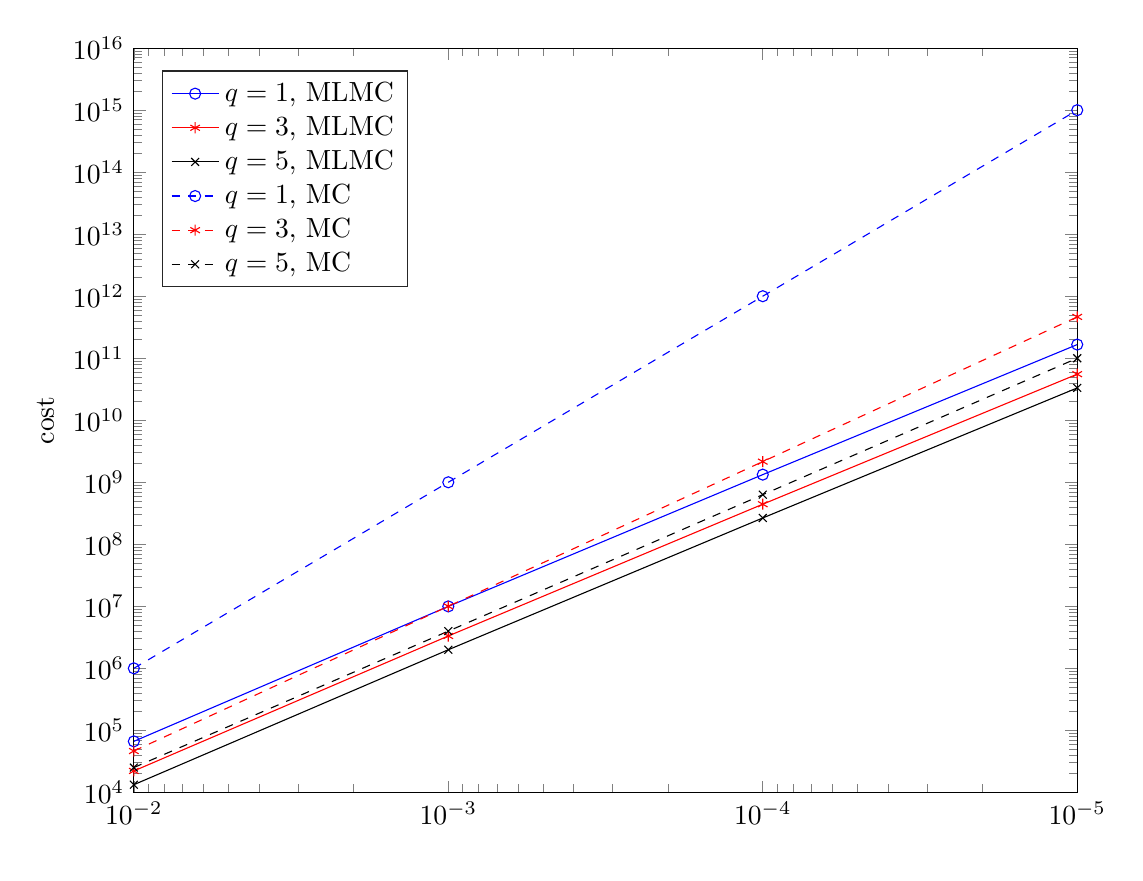
\begin{tikzpicture}

\begin{axis}[%
width=4.717in,
height=3.721in,
at={(0.791in,0.502in)},
scale only axis,
x dir=reverse,
xmode=log,
xmin=1e-05,
xmax=0.01,
xminorticks=true,
xlabel={$\epl$},
ymode=log,
ymin=10000,
ymax=1e+16,
yminorticks=true,
ylabel={cost},
axis background/.style={fill=white},
legend style={at={(0.03,0.97)},anchor=north west,legend cell align=left,align=left,draw=white!15!black}
]
\addplot [color=blue,solid,mark=o,mark options={solid}]
  table[row sep=crcr]{%
0.01	66438.5618977472\\
0.001	9965784.28466209\\
0.0001	1328771237.95494\\
1e-05	166096404744.368\\
};
\addlegendentry{$q = 1$, MLMC};

\addplot [color=red,solid,mark=asterisk,mark options={solid}]
  table[row sep=crcr]{%
0.01	22146.1872992491\\
0.001	3321928.09488736\\
0.0001	442923745.984982\\
1e-05	55365468248.1227\\
};
\addlegendentry{$q = 3$, MLMC};

\addplot [color=black,solid,mark=x,mark options={solid}]
  table[row sep=crcr]{%
0.01	13287.7123795495\\
0.001	1993156.85693242\\
0.0001	265754247.590989\\
1e-05	33219280948.8736\\
};
\addlegendentry{$q = 5$, MLMC};

\addplot [color=blue,dashed,mark=o,mark options={solid}]
  table[row sep=crcr]{%
0.01	1000000\\
0.001	1000000000\\
0.0001	1000000000000\\
1e-05	1e+15\\
};
\addlegendentry{$q = 1$, MC};

\addplot [color=red,dashed,mark=asterisk,mark options={solid}]
  table[row sep=crcr]{%
0.01	46415.8883361278\\
0.001	10000000\\
0.0001	2154434690.03189\\
1e-05	464158883361.279\\
};
\addlegendentry{$q = 3$, MC};

\addplot [color=black,dashed,mark=x,mark options={solid}]
  table[row sep=crcr]
%	\caption{Theoretical cost as a function of the desired accuracy and of the order $q$ of the numerical integrator if Monte Carlo or MLMC are applied.}
%	\label{fig:MLMCtheory}
%\end{figure}

%\subsubsection{Numerical example}
%We consider the Fitzhug-Nagumo problem \eqref{eq:FitzNag} and we aim to verify the cost of MLMC with respect to standard Monte Carlo for the estimation of the expectation of the solution at final time when applying the numerical method \eqref{probabilityODE}. We consider the case $q = p = 1$, using as a deterministic integrator the explicit Euler method. Hence, once a value of accuracy $\epl$ is requested, the number of stages $L$ as well as the time steps $h_l, l = 0, \ldots, L$, are imposed using \eqref{LCaseOne} and \eqref{hLeps}. In order to set up the standard Monte Carlo method, we consider the cost obtained in the MLMC simulation, denote by $\hat C$ and impose it to be equal for the standard Monte Carlo. In order to obtain a good balance between the error terms in \eqref{MSEMC} we impose
%\begin{equation}
%\begin{aligned}
%	\frac{T}{h} M &= \hat C, \\
%	M &= \ceil{h^{-2q}},
%\end{aligned}
%\end{equation}
%thus obtaining for the time step
%\begin{equation}
%	h = \left(\frac{T}{\hat C}\right)^{1 / (2q + 1)}.
%\end{equation}
%In this way, the computational cost for MLMC and standard Monte Carlo are imposed to be artificially equal and the two methods can be compared for their weak error with respect to an accurate solution. We impose for MLMC four values of accuracy $\epl = 0.1, 0.01, 0.001, 0.0001$, and apply the aforementioned technique to compare MLMC and Monte Carlo. Results (Figure \ref{fig:MLMCpractice}) show that imposing $L$ and $h_l, l = 0, \ldots, L$ as above the obtained accuracy in the same order of magnitude as $\epl$. Furthermore, the obtained accuracy is smaller for MLMC than MC if the cost 
%
%\begin{figure}
%	\centering
%	\resizebox{0.6\linewidth}{!}{% This file was created by matlab2tikz.
%
%The latest updates can be retrieved from
%  http://www.mathworks.com/matlabcentral/fileexchange/22022-matlab2tikz-matlab2tikz
%where you can also make suggestions and rate matlab2tikz.
%
\definecolor{mycolor1}{rgb}{0.00000,0.44700,0.74100}%
%
\begin{tikzpicture}

\begin{axis}[%
width=4.717in,
height=3.721in,
at={(0.791in,0.502in)},
scale only axis,
xmode=log,
xmin=100,
xmax=10000000000,
xminorticks=true,
xlabel={Cost},
ymode=log,
ymin=0.0001,
ymax=1,
yminorticks=true,
ylabel={Accuracy},
axis background/.style={fill=white},
legend style={legend cell align=left,align=left,draw=white!15!black}
]
\addplot [color=mycolor1,solid,mark=o,mark options={solid}]
  table[row sep=crcr]{%
480	0.25110925\\
56896	0.0261217025\\
5237760	0.002328838\\
1878933504	0.000163954625\\
};
\addlegendentry{MLMC};

\addplot [color=red,solid,mark=o,mark options={solid}]
  table[row sep=crcr]
%	\caption{Accuracy of MLMC and standard Monte Carlo for the FitzHug-Nagumo problem with fixed cost.}
%	\label{fig:MLMCpractice}
%\end{figure}

